\documentclass[12pt]{book}

\usepackage{hyperref}
\def\chapterautorefname{Chapter}
\def\sectionautorefname{Section}
\def\subsectionautorefname{Section}
\def\subsubsectionautorefname{Section}

\usepackage{algorithm}
\usepackage{algpseudocode}
\algrenewcommand\algorithmicrequire{\textbf{Input:}}
\algrenewcommand\algorithmicensure{\textbf{Output:}}
\algnewcommand\Not{\textbf{not} }
\newcommand{\algorithmautorefname}{Algorithm} % autoref

\usepackage{adjustbox}
\usepackage[headings]{fullpage}
\usepackage{xargs}
\usepackage{xspace}
\usepackage[doublespacing]{setspace}

%%%%%%%%%%%%%%%%%%%%%%%%%%%%%%%%%%%%%%%%%%%%%%%%%%%%%%%%%%%%%%%%
\usepackage{graphics, subfigure, float, algpseudocode, algorithm}
\usepackage{fp, calc}
\usepackage{mdwlist}
\usepackage{amscd,amsthm}
\usepackage{amsfonts, amssymb}
\usepackage{amsmath}
%\usepackage{fullpage} % Should come right after \documentclass kommen




% Special symbols, etc.
% \usepackage{amssymb,amsbsy,latexsym}
% \usepackage{amsmath}

%\usepackage{hyperref}
%\def\url#1{URL-MISSING
%\usepackage[sectionbib]{chapterbib}
%\usepackage[style=alphabetic,backend=biber]{biblatex}
%\usepackage[refsection=chapter,style=alphabetic,backend=bibtex]{biblatex}
%\addbibresource{IntOpt-and-Lattices.bib}

% Encoding settings
% \usepackage[latin1]{inputenc}
% %\usepackage[ngerman]{babel}
% \usepackage[T1]{fontenc} % IMPORTANT: Before loading fonts
% %\usepackage{mathpple} % Palatino Fonts
% \usepackage{fourier}
% \usepackage{bm}
% AMS Math packages



% Bibliography
%\usepackage[authoryear]{natbib}

%\usepackage{natbib}

%\usepackage{bibgerm}
%\usepackage[numbers]{natbib}

%\usepackage{cite}

% Graphics
% \usepackage[dvips]{graphicx,epsfig,color}
%\usepackage{subfigure}
%\usepackage{pstricks}
%\usepackage{pst-node} 
% \usepackage{pst-plot} (MIGHT NEED)
%\usepackage{pst-math}
% \usepackage{pst-all} (MIGHT NEED)
%\usepackage{pst-3dplot}
% \usepackage{pstricks-add,pst-func} (MIGHT NEED)
% \newpsobject{showgrid}{psgrid}{subgriddiv=1,griddots=10,gridlabels=6pt} (MIGHT NEED)
% \usepackage{comment,verbatim}

\newtheoremstyle{theorem}{1em}{1em}{\slshape}{0pt}{\bfseries}{.}{ }{}
\theoremstyle{theorem}
\newtheorem{theorem}{Theorem}
\newtheorem*{theorem*}{Theorem}
\newtheorem{corollary}[theorem]{Corollary}
\newtheorem{proposition}[theorem]{Proposition}
\newtheorem{lemma}[theorem]{Lemma}
\newtheorem*{lemma*}{Lemma}
\newtheorem{conjecture}[theorem]{Conjecture}
\newtheorem{claim}[theorem]{Claim}

\algdef{SE}[SUBALG]{Indent}{EndIndent}{}{\algorithmicend\ }%
\algtext*{Indent}
\algtext*{EndIndent}

\theoremstyle{remark}
\newtheorem{remark}{Remark}
\newtheorem*{remark*}{Remark}
%\newtheorem{algorithm}{Algorithm}

\def\rem#1{{\marginpar{\raggedright\scriptsize #1}}}

\providecommand{\setN}{\mathbb{N}}
\providecommand{\setZ}{\mathbb{Z}}
\providecommand{\setQ}{\mathbb{Q}}
\providecommand{\setR}{\mathbb{R}}
\providecommand{\setC}{\mathbb{C}}
\providecommand{\setF}{\mathbb{F}}
\newcommand{\E}{\mathop{\mathbb{E}}}
% \renewcommand{\qedsymbol}{\includegraphics[scale=0.3][santaqed.png]}

\newcommand{\vol}{\textrm{vol}}
% \renewcommand{\span}{\textrm{span}}
\newcommand{\conv}{\textrm{conv}}
\newcommand{\cone}{\textrm{cone}}

% \psset{linewidth=1pt, arrowsize=6pt} (MIGhT NEED)
\floatstyle{ruled}
\newfloat{algorithm}{tbp}{loa}
\floatname{algorithm}{Algorithm}

%%%%%%%%%%%%%%%%%%%%%%%%%%%%%% Textclass specific LaTeX commands.
 \theoremstyle{definition}
 \newtheorem{definition}{Definition}
  \theoremstyle{plain}
  \newtheorem{lem}{Lemma}
  \theoremstyle{plain}
  \newtheorem{cor}{Corollary}
  \theoremstyle{plain}
  \newtheorem{thm}{Theorem}

%\newcounter{exercise}

\theoremstyle{definition}
%\newtheorem{definition}[theorem]{Definition}
\newtheorem{notation}[theorem]{Notation}
\newtheorem{example}[theorem]{Example}
%\newtheorem{remark}[theorem]{Remark}
\newtheorem{problem}[theorem]{Problem}

\newtheorem{openquestion*}{Open Question}
\theoremstyle{theorem}

%\newtheoremstyle{theorem}{1em}{1em}{\slshape}{0pt}{\bfseries}{.}{ }{}
%\theoremstyle{theorem}
%\newtheorem{theorem}{Theorem}
%\newtheorem{question}{Question}

        % \def\drawRect#1#2#3#4#5{
        %    \FPeval{\x2}{(#2) + (#4)} 
        %    \FPeval{\y2}{(#3) + (#5)} 
        %    \pspolygon[#1](#2,#3)(\x2,#3)(\x2,\y2)(#2,\y2)
        % }

% \psset{nodesep=0.8pt}

%% Takes care, that preview-latex shows a preview of this environment
\usepackage[displaymath,textmath,sections,graphics, subfigure, floats]{preview} 
%%\PreviewEnvironment{enumerate} % Attention: Do not use comma-seperated lists here 
%%\PreviewEnvironment{itemize}
%%\PreviewEnvironment{theorem} 
%%\PreviewEnvironment{lemma} 
%\PreviewEnvironment{myproblem}
%%\PreviewEnvironment{algorithm} 
%\PreviewEnvironment{defn} 
\PreviewEnvironment{center} 
%\PreviewEnvironment{pspicture} 
% -------
% REMARK: 
% IF Emacs crashes on start of Preview-latex, mark smaller regions and click on 
% Preview -> (or toggle) at point
% -------

% \definecolor{augpathgray}{gray}{0.5} % 0=black, 1=white

\usepackage{calrsfs} % changes mathcal symbols in math
\DeclareMathAlphabet{\pazocal}{OMS}{zplm}{m}{n}
\newcommand{\La}{\mathcal{L}}
\newcommand{\Lb}{\pazocal{L}}
\newcommand{\calI}{\pazocal{I}}
\newcommand{\poly}{\operatorname{poly}}
\newcommand{\disc}{\operatorname{disc}}
\newcommand{\p}{\mathsf{P}}
\newcommand{\Q}{\mathsf{Q}}
\newcommand{\R}{\mathsf{R}}
\newcommand{\Prec}{\mathsf{prec}}
\newcommand{\Intervals}{c\mathsf{-intervals}}
\newcommand{\dup}{\mathsf{dup}}
\newcommand{\Cmax}{C_{\mathsf{max}}}
\newcommand{\wjcj}{\sum w_j C_j}
%%%%%%%%%%%%%%%%%%%%%%%%%%%%%%%%%%%%%%%%%%%%%%%%%%

\usepackage{microtype}
\usepackage[T1]{fontenc}

\usepackage[font={sf}]{caption}
% \usepackage[subrefformat=parens]{subcaption} (MIGHT NEED)
\usepackage{multirow}

\usepackage{xcolor}
\usepackage{graphicx}
\graphicspath{{_build/}{figures/}}





% \usepackage{fancyhdr}
% \setlength{\headheight}{15.2pt}
% \pagestyle{fancy}
% \lhead{Max Willsey}
% % \chead[<even output>]{<odd output>}
% \rhead{\thechapter. \chaptername}

\usepackage{libertine}
\usepackage[scaled=.9]{DejaVuSansMono}

\allowdisplaybreaks


\def\mytitle{Improving Scheduling Algorithms via a Mathematical Perspective}
\def\myauthor{Sami Davies}
\def\year{2021}

\title{\mytitle}
\author{\myauthor}

% \input{macros}

\begin{document}
\pagestyle{empty}

% title and copyright pages
\begin{center}
  {\huge \mytitle}
  \vfill

  {\Large \myauthor}
  \vfill

  \begin{spacing}{1}
    A dissertation \\
    submitted in partial fulfillment of the \\
    requirements for the degree of
  \end{spacing}
  \vfill

  Doctor of Philosophy
  \vfill

  University of Washington \\
  \year
  \vfill

  Reading Commitee: \\
  Thomas Rothvoss, Chair \\
Anna Karlin \\
 Isabella Novik
  \vfill

  \begin{spacing}{1}
    Program Authorized to Offer Degree: \\
    Department of Mathematics
  \end{spacing}
  \clearpage

  \textcopyright{} Copyright \year\\
  \myauthor
  \clearpage
\end{center}

\pagestyle{plain}
\setcounter{page}{1}
\pagenumbering{roman}

% abstract page
\begin{center}
  University of Washington \\[1em]
  \textbf{Abstract}        \\[1em]
  \mytitle                 \\[1em]
  \myauthor                \\[1em]

  % Supervisory Committee: \\[-0.5em]
  % Luis Ceze, Chair \qquad
  % Adriana Schulz   \qquad
  % Zachary Tatlock  \\[-0.5em]
  Chair of the Supervisory Committee: \\[-0.5em]
  Thomas Rothvoss \\[-0.5em]
  Department of Mathematics
  \\[2em]
\end{center}
This document will discuss three problems that I worked on during my Ph.D. 
Chapter \ref{chapter: SC} contains my work on the Santa Claus problem, and
Chapters \ref{chapter: S1} and \ref{chapter: S2} contain my work on scheduling with precedence constraints and communication delays.
New algorithms for scheduling and resource allocation problems have far reaching implications, as problems in scheduling and resource allocation
are a foundational playground for studying computational hardness and are practically relevant.
% We see these implications in avenues that increase the productivity of businesses, 
% like dynamically allocating to the cloud; that speed up processes in computing, 
% like training deep neural networks; and that promote social equity, 
% like helping Boston public schools design so- cioeconomic conscious bus routes [MPST18, NHP+19, BDE+20]. 

In the \emph{Santa Claus problem}, Santa has a set of gifts, and he wants to distribute them among a set of children
so that the least happy child is as happy as possible. 
Child $i$ has value $p_{ij}$ for present $j$, where $p_{ij}$ is in $ \{ 0,p_j\}$.
A modification of Haxell's hypergraph matching argument by Annamalai, Kalaitzis, and Svensson gives a $12.33$-approximation algorithm for the problem.
In joint work with Thomas Rothvoss and Yihao Zhang, we introduce a matroid version of the Santa Claus problem. 
While our algorithm is also based on the augmenting tree by Haxell, the introduction
of the matroid structure allows us to solve a more general problem with cleaner methods.
Using our result from the matroid version of the problem, we obtain a $(4+\varepsilon)$-approximation algorithm for Santa Claus.

In scheduling theory, one of the most poorly understood, yet practically interesting, models is scheduling
in the presence of \emph{communication delays}.
Here,
if two jobs are dependent and scheduled on different machines,
then at least $c$ units of time must pass between their executions.
Even for the special case where an unlimited number of identical machines are available, the best known approximation ratio
for minimizing makespan is $O(c)$.
An outstanding open problem in the top-10 list by Schuurman and Woeginger (and its recent update by Bansal)
asks whether there exists a constant-factor approximation algorithm.
In joint work with Janardhan Kulkarni, Thomas Rothvoss, Jakub Tarnawski, and Yihao Zhang,
 we prove a $O(\log c \cdot \log m)$-approximation algorithm
for the problem of minimizing makespan
on $m$ identical machines; this work is presented in Chapter \ref{chapter: S1}.
Our approach is based on a Sherali-Adams lift of a linear programming relaxation
and a randomized clustering of the semimetric space induced by this lift. 
We extend our work to the related machines setting and study the objectives of minimizing makespan 
and minimizing the weighted sum of completion times. 
Here, we also obtain polylogarithmic approximation algorithms, and these results are presented in Chapter \ref{chapter: S2}.

\begin{spacing}{1.5}
  \tableofcontents
\end{spacing}

\chapter*{Acknowledgments}

To begin, it's hard for me to imagine a more capable and supportive advisor than Thomas. 
Thomas taught me a lot about how to approach problems, what to do when I get stuck, and when to move on.
He is also not only an exceptional researcher, but he always showed an incredible amount of patience, kindness, and humility in our work. 

I received a great deal of mentorship from Janardhan Kulkarni during my Ph.D, and I thank Jana for his continued 
honesty, guidance, and support as I move into postdoctoral life.
Several works in this thesis are joint with Yihao Zhang and Jakub Tarnawksi, both of whom I was fortunate to work with and learn from.
Jana and Jakub also hosted me at MSR during the summer of 2020; an experience for which I am grateful.
While our work is not featured in this thesis, I am grateful to my coauthors Cyrus Rashtchian and Miki Racz 
for their friendship and mentorship over the past several years.


I made many friends in the Math department and CS theory group (and the PLSE group too), and I thank the students and faculty of both 
for allowing me to fluidly move between the two at my whim. 
Throwing it way back, people who really encouraged me to go to grad school and then study TCS were
Bill Hrusa, Brendan Sullivan, Lev Reyzin, and Jeremy Kun.
I thank my family---especially my sister, Addie---for supporting me as I live far away and do something they don't really understand.
And lastly, to Max, thank you for helping me find balance in life over the past 5 years.


\begin{center}
    \textbf{DEDICATION}


\emph{to Mr. Raymond Kreiser}


\end{center}




\clearpage

\pagestyle{headings}
\setcounter{page}{1}
\pagenumbering{arabic}
\renewcommand{\chaptermark}[1]{\markboth{\sc{\chaptername\ \thechapter.\ #1}}{}}
\renewcommand{\sectionmark}[1]{\markright{\sc{\thesection.\ #1}}{}}
\chapter{Introduction and Background}



Many optimization problems can be modelled as linear programs of the form $\max_x\{c^T x | Ax \leq b\}$.
There are methods to solve linear programs efficiently and obtain a fractional solution, 
but often any valuable $x$ is integral. 
Finding optimal integral solutions is theoretically intractable, 
so instead we often take a fractional solution and devise some algorithm that \emph{rounds} 
the fractional solution to an integral one. 
The rounding algorithm is seen as decent if not too much is lost in the objective value from moving from the fractional solution to the integral one.


In designing linear program relaxations, we define that \emph{integrality gap} of an instance
to be the maximum ratio between the optimal objective value of the integral solution for that instance and the optimal objective value of 
the relaxation for that instance.
The integrality gap is the standard way of measuring 
how well a linear program actually captures the problem. 


We accept that it is extremely likely that there exists a separation 
between the set of ``easy'' and the set of ``hard'' problems, i.e. those for which we can always find an optimal solution in time polynomial in the 
size of the problem, and those for which we cannot. 
Instead, we work towards obtaining approximate solutions efficiently. 
An \emph{$\alpha$-approximation algorithm} for an optimization problem is
an algorithm which given any instance of the problem is guaranteed to return a solution whose value is
within an $\alpha$ factor 
of the value of the optimal solution, within time polynomial in the size of the instance.

Designing LPs with small integrality gap (small depends on the target approximation factor) can be difficult. 
One normally begins by writing down the basic constraints that arise from the problem statement; let me call this the basic LP for now. 
To judge the quality of that basic LP, the next step is to try and think of instances that might lead to a larger-than-desired integrality gap.
If indeed there is an instance certifying that the integrality gap is large, then one has to come up 
with additional constraints to add the LP that will make the eliminate the bad instances. 
Even if there is an LP for which there are no obvious integrality gap instances, it might be that 
it is difficult to come up with a way to round  
Sometimes this ad hoc approach works relatively well, in that coming up with constraints to eliminate bad instances 
is not too difficult given previous work or intuition or luck\footnote{In the Santa Claus problem, this ad hoc approach works well enough for our purposes!}.
But other times, one either 
\begin{itemize}
\item(a) enters a vicious cycle of thinking up new integrality gap instances, then adding new constraints to get rid of the instances, 
then thinking up more integrality gap instances, and so on and so forth until you die, or
\item(b) (potentially after repeitions of (a)) is eventually unable to come up with integrality gap instances, 
but also cannot do anything useful in the rounding or analysis. 
\end{itemize}
Appealing though these options may be, hierarchies can help avoid them. 



Talk about hierarchies. Sherali Adams, constructing the compact LP, integrality gaps, use of triangle inequality in ARV.


A (rambly, yet) brief sidebar follows.
Problems that are considered in theoretical computer science from the measurement of approximation algorithms 
are often motivated from practical situations. 
But it is worth noting that in the definition of an $\alpha$-approximation algorithm, 
we require that the algorithm obtains a solution whose value is only $\alpha$ off for \emph{any} input.
Depending on your persuasion, this may seem like a very strong definition, and maybe impractical... 
perhaps the inputs that make algorithm design difficult are contrived or never really arise in practice. 
So we have a---at first glance---strange juxtaposition, where we motivate a problem by saying it has practice,
but we measure our success with a potentially impractical definition.
From my perspective, the above is missing the point. 
The design and analysis of approximation algorithms is, to me and to many others in the field, all about the math.
Specifically, it is about studying what mathematical structures we can superimpose onto a hard problem in order to make a little more sense 
of why it is indeed hard. 
For that reason, runtime, so long as it is polynomial in the instance size, is not a large concern in the works featured here.
Though it might be of concern to me someday, and there is a lot of meaningful work in approximation algorithms, TCS, and beyond that 
takes runtime, memory, input characteristics, and other practical concern into consideration.




\bigskip

We focus on two specific NP-hard problems in this paper: Santa Claus, also known as Restricted Max-Min Fair Allocation, and scheduling 
with precedence constraints and communication delays.

\section{The Santa Claus problem}

In the \emph{Santa Claus problem}, the objective is to allocate gifts to children in such a way that the minimum value of any child is maximized. 
We assume that child $a \in A$ has value $p_{a,i}$ for item $i \in I$ and that a child's value is the sum of the values of the gifts they receive. 
Formally, we seek an assignment $\phi: I \rightarrow A$ such that $\min_{a \in A} \sum_{\phi^{-1}(a)} p_{a,i}$ is maximized. 
Let $m$ denote the number of children and $n$ the number of gifts. 
In Santa Claus, we assume that $p_{a,i} \in \{0,p_i\}$, i.e if two children both want to receive a gift, then they both value it equally.
We will refer to the unrestricted version of MMFA occasionally for background, 
where in the unrestricted version $p_{a,i}$ does not necessarily need to belong to $\{0,p_i\}$.

\subsection{Previous work on Santa Claus}


It is NP-hard to approximate Santa Claus within 
a factor less than 2 \cite{BezakovaD05}. 
Though interestingly, the known approximation factors for upper bounds wildly differ between the 
restricted and unrestricted cases. 
Before our work, constructive methods for both the restricted and unrestricted versions of 
Max-Min Fair Allocation in some way use the existence of a solution to an exponentially large
\textit{configuration linear program}  \cite{SantaClaus-BansalSviridenko-STOC2006, AlgoForSantaClaus-AnnamalaiKalaitzisSvenssonSODA15, AS10, MaxMinFairAllocation-ChakrabartyChuzhoyKhannaFOCS09, ChengM18}.
 
%The CLP is a strong relaxation with an exponential number of variables, but it perhaps does not invoke much intuition,
%as it is brute forcing which bundles of gifts satisfy children. 
For a CLP with objective value $T$, 
the variables in the CLP take the form $x_{a,C}$, 
which represents whether agent $a$ receives the subset of items $C \in  \pazocal{C}(a,T)$, 
those sets of items bringing agent $a$ at least value $T$:
\begin{align*}(CLP) \qquad
\sum_{C \in \pazocal{C}(a,T)} x_{a,C} &\geq 1  \qquad \forall a \in A \\
\sum_{C: i \in C} \sum_{a} x_{a,C} &\leq 1 \qquad \forall i \in I \\ 
x &\geq 0.
\end{align*}

The CLP was introduced by Bansal and Sviridenko when studying the Santa Claus problem. 
They use it to give an $O(\log \log m / \log \log \log m)$- approximation for the Santa Claus problem  \cite{SantaClaus-BansalSviridenko-STOC2006}. 
Since then, progress has been made towards better constant factor approximations for the Santa Claus problem, 
with Feige proving an (unspecified constant) $O(1)$-approximation and Annamalai, Kalaitzis, and Svensson proving 
a 12.3-approximation \cite{ConstantIntegralityGapSantaClaus-Feige-SODA2008, AlgoForSantaClaus-AnnamalaiKalaitzisSvenssonSODA15}
The CLP for the Santa Claus problem has an integrality gap of $3.808$ \cite{CM19}. 

In contrast, the CLP for unrestricted Max-Min Fair Allocation has an integrality gap of $\Omega(\sqrt{m})$. 
Asadpour and Saberi give an $O(\log^3 m \sqrt{m})$-approximation through a beautiful randomized algorithm. 
Chakrabarty, Chuzhoy, and Khanna cleverly beat the $\sqrt{m}$ gap to obtain an $\tilde{O}(n^{\varepsilon})$-approximation 
in $n^{1/\varepsilon}$ time for $\varepsilon =\Omega \left (  \log \log n / \log n \right )$
by iteratively using solutions to the LP, 
whose gaps become smaller in each iteration\footnote{
Note that some results are in terms of $m$, and some in terms of $n$. Though in general
we think of $n$ as much larger than $m$, and in fact, 
the results of Chakrabarty, Chuzhoy, and Khanna hold replacing $n$ with $m$ for constant $\varepsilon.$
}. 
From these works, it is helpful to note that 
the algorithms rely on assigning heavy and light pairs, meaning those with large versus small $p_{a,i}$,
differently \cite{AlgoForSantaClaus-AnnamalaiKalaitzisSvenssonSODA15,MaxMinFairAllocation-ChakrabartyChuzhoyKhannaFOCS09}. 
Similar ideas have been used in Makespan Scheduling \cite{MakespanScheduling-Svensson-STOC11, SchedulingUnrelatedParallelMachines-LenstraShmoysTardos-FOCS87}.


More generally, studying Max-Min Fair Allocation can be viewed from the lens of investigating sufficient conditions for 
perfect matchings in bipartite hypergraphs. 
A hypergraph $\pazocal{H} = (V \dot\cup W, \pazocal{E})$ is called bipartite if for all
$e \in \pazocal{E}$, $|e \cap V|=1$, and hyperedges $F \subset \pazocal{E}$ form a (left) perfect matching 
if they are disjoint and every node in $V$ is contained in exactly one edge in $F$.
In particular, a solution to the CLP is a fractional perfect matching on the hypergraph 
$ \left(A \dot\cup I, \bigcup_{a \in A}\pazocal{C}(a,T) \right)$.  
Finding perfect matchings in bipartite hypergraphs is in general NP-hard, though
Haxell's condition defines a sufficient condition:
\begin{theorem} \cite{HypergraphMatchingsHaxell95}
Let $\pazocal{H} = (V \dot\cup W, \pazocal{E})$ be a bipartite hypergraph with $|e| \leq r$ for all $e \in \pazocal{E}$.
Then either $\pazocal{H}$ contains a (left) perfect matching or there are subsets $V' \subset V$ and $W' \subset W$
so that all hyperedges incident to $V'$ intersect $W'$ and $|W'| \leq (2r-3)(|V'|-1)$.
\end{theorem}
While the proof of Haxell's condition relies on a potentially exponential time argument, 
Annamalai made the argument polynomial by restricting edge sizes to be uniform and allowing some slack in the inequality \cite{FindingPerfectMatchingsInHypergraphs-Annamalai-SODA16}.
His argument, in addition to the one made in the 12.3-approximation algorithm by Annamalai, Kalaitzis, and Svensson,
take Haxell's argument and make it polynomial by introducing an augementing tree. 
This generalizes the notion of an augmenting path used to find a maximum matchings in bipartite graphs.
Instead of swapping every other edge in an augmenting path, as is the case for a bipartite graph,
the augmenting tree swaps sets of alternating hyperedges to find more space in the hypergraph.








% Given a set of agents and a set of goods, a natural question 
% is how does one distribute the goods in a way that is fair? 
% While the notion of algorithmic fairness is now a rich area of theoretical computer science, 
%  Max-Min Fair Allocation presents a simple notion of fairness that leads to a practical combinatorial optimization problem.
%  In \emph{Restricted Max-Min Fair Allocation},
% the objective is to allocate items to agents in such a way that the minimum value of any agent is maximized.
% We assume that agent $a \in A$ has value $p_{a,i}$ for item $i \in I$, where $p_{a,i} \in \{0,p_i\}$ for $p_i \in \mathbb{Z}^+$, and that an agent's value is the sum of the values of the items they receive.
% Formally, we seek an assignment $\phi :I \rightarrow A $ such that $\min_{a \in A} \sum_{i \in \phi^{-1}(a)}p_{a,i}$ is maximized. 

% Let $m$ denote the number of agents and $n$ the number of items.
% This problem is affectionately known as the Santa Claus problem, 
% with lingo swapping the terms ``agents'' and ``items'' for ``children'' and ``presents''.
% More generally, 
% Restricted Max-Min Fair Allocation can be viewed
% %  from the lens of investigating
%  as a problem of finding sufficient conditions for 
% perfect matchings in bipartite hypergraphs. 
% A hypergraph $\mathcal{H} = (V \dot\cup W, \mathcal{E})$ is called bipartite if for all
% $e \in \mathcal{E}$, $|e \cap V|=1$, and hyperedges $F \subset \mathcal{E}$ form a (left) perfect matching 
% if they are disjoint and every node in $V$ is contained in exactly one edge in $F$.
% In particular, a solution to the configuration linear program is a fractional perfect matching on the hypergraph 
% $ \left(A \dot\cup I, \bigcup_{a \in A}\mathcal{C}(a,T) \right)$.  
% While finding perfect matchings in bipartite hypergraphs is in general NP-hard, 
% in some classes of hypergraphs they can be found efficiently~\cite{AKS17, Annamalai15}.
% Such algorithms generalize the notion of an augmenting path used to find a maximum matchings in bipartite graphs.


\subsection{Our contribution }
In my work on the Santa Claus problem with Thomas Rothvoss and Yihao Zhang,
we exploit an underlying matroid to design a clean bipartite hypergraph matching algorithm \cite{DaviesRZ20}. 
This leads to an improved approximation factor (from 12.3 to $4+ \varepsilon$) compared to the solution of a new linear program relaxation
\footnote{After obtaining our results, 
we learned that Cheng and Mao simultaneously and independently obtained 
a $6 + \varepsilon$ approximation to the Santa Claus problem
by altering the algorithm by Annamalai, Kalaitzis and Svensson \cite{ChengM18}.  
Using ideas established by Asadpour, Feige, and Saberi, they further improved this
to a $4 + \varepsilon$ approximation \cite{CM19, SantaClaus-AsadpourFeigeSaberi-APPROX2008}.}.

We build off the idea of separating gifts by their values by designating a gift $i$ as either large or small, depending on its value $p_i$. 
Our linear program has only $O(n^2)$ many variables and constraints and uses this distinction between large and small gifts. 
In particular, we introduce an expansion constraint, 
forcing children who do not entirely receive a large gift to fractionally receive at least $T$ small gifts, 
for $T$ the optimal objective value. Let
$I_L := \{ i \in I \mid p_i > \delta_2 T\}$ denote the large gifts
and $I_S := \{ i \in I \mid p_j \leq \delta_1 T\}$ denote the small gifts
for constants $0 < \delta_1 \leq \delta_2 < 1$ such that
% For fixed parameters $1 \geq \delta_2 \geq 1/4 > \delta_1 \geq 0$, where 
all gifts have values in $[0,\delta_1  T] \cup (\delta_2  T,T]$. 
$A_i$ denotes the set of children who wish to receive gift $i$, in other words the set of $a \in A$ such that $p_{a,i} \neq 0$.
Let $P(T,\delta_1,\delta_2)$ be the set of vectors $z \in \mathbb{R}_{\geq 0}^{J \times M}$ satisfying
\begin{eqnarray*}\label{eq:CompactLPforSC} \qquad
        \sum\limits_{i \in I_S: a \in A_i} p_i z_{ai} &\geq& T \cdot \Big( 1-\sum_{i \in I_L: a \in A_i} z_{ai}\Big)  \qquad \forall a \in A \\
        \sum\limits_{a \in A_j}z_{ai} &\leq& 1 \hspace{4.0cm} \forall i \in I \\
        z_{ai} &\leq& 1-\sum_{i' \in I_L: a \in A_{i'}} z_{ai'} \hspace{1.5cm} \forall i \in I_S \; \forall a \in A_i.
\end{eqnarray*}


The separation between large and small gifts was critical for our approach as it allowed us to define an underlying matroid.
Recall a matroid is a structure generalizing the notion of linear independence in vector spaces,
and in particular their independent sets have useful exchange properties. 
Formally, $\pazocal{M} = (X,\pazocal{I})$ is a matroid with groundset $X$ and 
independent sets $\pazocal{I} \subseteq 2^X$ if the following hold:
\begin{itemize}
\item \emph{Non-emptyness}: $\emptyset \in \pazocal{I}$; 
\item \emph{Monotonicity}: For $Y \in \pazocal{I}$ and $Z \subseteq Y$ one has $Z \in \pazocal{I}$; 
\item \emph{Exchange property}: For all $Y,Z \in \pazocal{I}$ with $|Y| < |Z|$ there is an element $z \in Z \setminus Y$ so that $Y \cup \{ z\} \in \pazocal{I}$.
\end{itemize}
The bases of a matroid, denoted by $\pazocal{B}(\pazocal{M})$, are all inclusion-wise maximal independent sets, and
the convex hull of all bases is called the base polytope, denoted by $P_{\pazocal{B}(\pazocal{M})} := \text{conv}\{ \chi(S) \in \{0,1\}^X \mid S\text{ is basis}\}$,
where $\chi(S)$ is the characteristic vector of $S$.


Now consider a bipartite graph $G = (V \dot{\cup} W,E)$ with ground set $V$ on one side and
a set of resources $W$ on the other side; each resource $w \in W$ has
value $p_w \geq 0$. 
We define the problem \emph{Matroid Max-Min Allocation}, 
where the goal is to find a basis $S \in \pazocal{B}(\pazocal{M})$ and an 
assignment $\sigma : W \to S$ with $(\sigma(w),w) \in E$ so that $\min_{v \in S} \sum_{w \in \sigma^{-1}(v)} p_w$ 
is maximized. 
For $T \geq 0$ the target objective function value, 
we define a linear programming relaxation $Q(T)$ as the set of vectors 
$(x,y) \in \mathbb{R}_{\geq 0}^X \times \mathbb{R}_{\geq 0}^E$
satisfying the constraints:
\begin{eqnarray*}
 x \in P_{\pazocal{B}(\pazocal{M})};& \quad 
 \sum_{w \in N(v)} p_wy_{vw} \geq T \cdot x_v \;  \forall v \in V;\\
  \quad  y(\delta(w)) \leq 1 \;
  \forall w \in W;& \qquad \qquad \qquad y_{vw} \leq x_v \; \forall (v,w) \in E.
\end{eqnarray*} 

Here, the decision variable $x_v$ expresses whether element $v$ should be part of the basis, and
$y_{vw}$ expresses whether resource $w$ should be assigned to element $v$. We abbreviate 
$N(v)$ for the neighborhood of $v$ and $y(\delta(w))$ for $\sum_{v : (v,w) \in E} y_{vw}$.
Our main technical result is the folllowing: 
\begin{theorem}\label{thm:MainMatroidAlgorithm} \cite{DaviesRZ20}
Suppose $Q(T) \neq \emptyset$ and membership in the matroid can be tested in time polynomial in $n$.
Then for any $\varepsilon>0$ one can find
 \[
   (x,y) \in Q \left (
    \left (\frac13 - \varepsilon \right ) \cdot T - \frac13 \cdot \max_{w \in W} p_w \right )
 \] 
with both $x$ and $y$ integral in time $n^{\Theta_{\varepsilon}(1)}$, where $n := |V| + |W|$. 
\end{theorem}


Viewing the set of children and gifts as parts of a bipartite graph, 
the sets of children which can be given a large gift forms a matchable set matroid, $\pazocal{M}$.
Thus children who do not receive a large gift form bases of $\pazocal{M}^*$, the co-matroid of $\pazocal{M}$.
Set $\delta_1$ so that $\delta_1 \cdot T$ is the largest gift value that is at most
$\frac14 \cdot T$, and set $\delta_2$ so that $\delta_2 \cdot T$ is the smallest gift value that is at least $\frac14 \cdot T$. 
In an instance of the Santa Claus problem where the optimal integral solution has value $T$, 
we transform a solution in $P(T,\delta_1,\delta_2)$ into a solution in $Q(T)$, with $\max_{w \in W} p_w = \delta_1 \cdot T$.

By using properties of matroids, 
we simplify a bipartite hypergraph matching algorithm, which builds an augmenting tree,
of Annamalai, Kalaitzis, and Svensson to find an assignment of small gifts to a basis of $\pazocal{M}^*$ \cite{AlgoForSantaClaus-AnnamalaiKalaitzisSvenssonSODA15}.
Using Theorem~\ref{thm:MainMatroidAlgorithm}, each child receiving only small gifts has value at least
$\left (\frac13 - \varepsilon \right ) \cdot T - \frac13 \cdot \delta_1 \cdot T \geq \left (\frac14 - \varepsilon \right ) \cdot T$. 
The remaining children who received no small gifts get a single large gift, with value at least $\delta_2 \cdot T \geq \frac14 \cdot T$,
guaranteeing every child at least $\frac14 - \varepsilon$ of the optimal value.
Interestingly, in the case where the distribution of gift values is bimodal and the gap between $\delta_1$ and $\delta_2$ is large, 
our approximation factor improves.
In the most extreme case when gift values are either 1 or $T$, 
our algorithm returns a $3 + \varepsilon$ approximation. 



% We alter an algorithm from [cite] which given a bipartite graph $G=(U,V,E)$, with $U$ the ground set of a matroid and $V$ unit-valued resources we wish to allocate to $U$, uses hypergraph matching techniques to find a basis $S$ of a matroid and a hypergraph matching $M$ with large enough edges covering $S$. Applying this more general framework to $\mathcal{M}^*$, we find a set of children which will only receive small gifts, and an assignment of small gifts to them. Properties of matroids and the the matroid polytope are essential in our construction a clean, correct argument.

% Just as in [cite], we construct an \textit{augmenting tree}. 
% This is a collection of hyperedges found layer by layer, where every other layer belongs in the current hyper matching. algorithm swaps sets of edges in the augmenting tree to find more space in the hypergraph. The edges are swapped in such a way that the set of children covered by the matching is always independent with respect to the matroid.





\section{Scheduling with Communication Delays} 


Distributing tasks onto processors occurs in many areas of computing.
Frequently, some tasks use as their inputs the outputs of other tasks. 
The cost of transferring data between processors can be expensive, 
e.g. in data center scheduling and Deep Neural Network training~\cite{coflow, zhao2015rapier}. 
This dependence and latency in scheduling is modelled with precedence constraints and communcation delays.

% The above precedence-constrained scheduling problem models the task of distributing workloads onto multiple processors or servers, which is ubiquitous in computing. This basic setting takes the dependencies between work units into account, but not the data transfer costs between machines, which is critical in applications. A precedence constraint j ≺ j′ typically implies that the input to j′ depends on the output of j. In many real-world scenarios, especially in the context of scheduling in data centers, if j and j′ are executed on different machines, then the communication delay due to transferring this output to the other machine cannot be ignored. This is an active area of research in applied data center scheduling literature, where several new abstractions have been proposed to deal with communication delays [CZM+11, GFC+12, HCG12, SZA+18, ZZC+12, ZCB+15, LYZ+16]. Another timely example is found in the parallelization of Deep Neural Network training (the ma- chines being accelerator devices such as GPUs, TPUs, or FPGAs). There, when training the network on one sample/minibatch per device in parallel, the communication costs incurred by synchronizing the weight updates in fact dominate the overall running time [NHP+19]. Taking these costs into account, it turns out that it is better to split the network onto multiple devices, forming a “model- parallel” computation pipeline [HCB+19]. In the resulting device placement problem, the optimal split crucially depends on the communication costs between dependent layers/operators.



Given a set of $n$ jobs, and a set of $m$ machines on which the jobs can be performed, 
scheduling algorithms find an assignment of jobs to machines and time slots.
The inclusion of \emph{precedence constraints} model the flow of jobs as a directed acyclic graph, where 
 if there is an edge in the DAG from $j_1$ to $j_2$, denoted $j_1 \prec j_2$, then $j_1$ must be completed before any machine can start to process $j_2$.
The inclusion of  \emph{communication delays} model the latency between dependent jobs, 
where if $j_1 \prec j_2$ and $j_2$ is performed on a different machine than $j_1$, then at least $c_{j_1,j_2}$ time 
units must pass after the completion of $j_1$ before any machine can start to process $j_2$.
The \emph{makespan} of a schedule is the time that the last machine processes its final job.

The PI  and her coauthors, Janardhan Kulkarni, Thomas Rothvoss, Jakub Tarnawski, and Yihao Zhang, have been studying the problem 
of scheduling  with 
precedence constraints and uniform communication delays, which is when $c_{j_1,j_2}=c$ for all $j_1,j_2$, on identical machines. 
In the identical machine setting, all machines have the same speed and are able to process every job. 
% In the objective of minimizing makespan, where the makespan is denoted $C_{\textrm{max}}$ for maximum completion time.
Before their work, simple arguments obtained $O(c)$-approximations for the objective of minimizing makespan~\cite{GrahamListScheduling1966, GiroudeauKMP08}.
While there are tighter bounds when $c=1$, little else was known for when $c$ is large, which is the parameter setting arising in practice~\cite{MunierKonig, HanenMunier73Apx}.
Obtaining better algorithms to the problem is in a list of the top 10 open problems in scheduling theory that was proposed by Schuurman and Woeginger~\cite{SW99a}.
More recently in a 2017 survey talk, Bansal described scheduling with precedence constraints and communication delays 
as ``not understood at all" and ``almost completely open"~\cite{Bansalmapsp}.

% The PI has worked on scheduling in the presence of precedence constraints and communication delays
%  with Janardhan Kulkarni, Thomas Rothvoss, Jakub Tarnawski, and Yihao Zhang. 
% For the base problem of $P_{\infty} \mid p_j=1, c \mid C_{\textrm{max}}$
% (minimizing makespan with unit processing times and communication delays of length $c$ on arbitrarily many machines),
The PI and her coauthors obtain a $O(\log(m) \cdot \log(c))$-approximation algorithm for the uniform communication delays problem on identical machines, 
making significant progress on the question posed by Schuurman and Woeginger~\cite{DKRTZ20}. 
% These results extend to include arbitrary processing times and a fixed number of machines.
They use a \emph{Sherali-Adams hierarchy} of a linear program, 
which introduces additional variables and constraints to obtain a tighter relaxation.
% , in order to obtain 
% a locally consistent probability distribution on pairs of jobs.
Using the LP solution, they construct a semimetric on the set of jobs, where jobs close in the semimetric are likely to be scheduled on the same machine
 and within $c$ time slots from each other. 
Equipped with a semimetric, the authors design an algorithm that uses as a subroutine a clustering algorithm by Calinescu, Karloff, and Rabani to schedule a subset of jobs~\cite{DBLP:journals/siamcomp/CalinescuKR04}.
%  takes as input the set of jobs that have completion time in a $O(c/ \log(c))$-length interval
% according to the LP solution and
% schedules a constant fraction of these jobs 
% while respecting precedence constraints~\cite{CKR01}. 
Repeating this iteratively and inserting $c$ idle time slots between each iteration accounts for the communication delay between jobs in different iterations.

The PI and her coauthors also obtained polylogarithmic approximation algorithms for the more general setting of
% of scheduling with precedence constraints and communication delays on 
related machines with the objective of minimizing the \emph{weighted sum of completion times}~\cite{DaviesKRTZ21}.
This objective is minimizing $\sum_j w_j C_j$, for $w_j$ the weight of job $j$, given as input, and
$C_j$ the completion time of job $j$.
% (referred to as $Q \mid p_j=1, c \mid  \sum_j w_j C_j$, for $C_j$ the completion time of job $j$).
In the related machine setting, the set of machines are partitioned into speed classes, where machines in speed class $\ell$
process job $j$ in time $p_j / s_\ell$.
% Nothing was known for this setting before our work.
This work generalizes the Sherali-Adams framework established in their previous paper, though there are new technical challenges.
For the objective of minimizing makespan, it was sufficient to determine in which $c$-length time interval a job is scheduled. 
However, for the weighted sum of completion times objective, this is not careful enough; jobs that have very small fractional completion time by the LP 
must be scheduled very early.
Additionally, as opposed to the identical machines setting, the problem now involves assigning jobs to speed classes.
The authors introduce more constraints into their LP and prove stronger structural insights about the Sherali-Adams solution.

We consider the problem of scheduling jobs with precedence constraints on related machines
to minimize the weighted sum of completion times,
in the presence of {\em communication delays}.
In this setting,
denoted by $\Q \mid \Prec, c \mid \sum w_jC_j$,
if two dependent jobs are scheduled on different machines,
then at least $c$ units of communication delay time must pass between their executions.
Our main result is an $O(\log^4 n)$-approximation algorithm for the problem.
As a byproduct of our result, we also obtain an $O(\log^3 n)$-approximation algorithm for the problem of minimizing makespan  $\Q \mid \Prec, c \mid C_{\textrm{max}}$, which improves upon the $O(\log^5 n/\log \log n)$-approximation algorithm due to a recent work of  Maiti et al.~\cite{MRSSV}.



[ADD LIKE 2 MORE PAGES ABOUT SCHEDULING IN HERE]
\chapter{Santa Claus}\label{chapter: SC}
% \\ {\small Last changes: \today}

\section{Introduction}

Formally, the \emph{Santa Claus} problem takes as input a set $M$ of children, a set $J$ of gifts,
and values $p_{ij} \in \{ 0,p_j\}$ for all $i \in M$ and $j \in J$. In other words, a child is
only interested in a particular subset of the gifts, but then its value only depends on the
gift itself. The goal is to find an assignment $\sigma : J \to M$ of gifts to children so that
$
  \min_{i \in M} \sum_{j \in \sigma^{-1}(i)} p_{ij}
$
is maximized.

The first major progress on this problem is due to Bansal and Sviridenko~\cite{SantaClaus-BansalSviridenko-STOC2006}, who showed a $O(\log \log n / \log \log \log n)$-approximation based on rounding a \emph{configuration LP}. The authors of \cite{SantaClaus-BansalSviridenko-STOC2006} also realized that in order to obtain a $O(1)$-approximation, it suffices to answer 
a purely combinatorial problem: show that
in a uniform bipartite hypergraph with equal degrees on all sides, there is a left-perfect matching that selects a constant fraction of nodes from original edges.
This question was affirmatively answered by Feige~\cite{ConstantIntegralityGapSantaClaus-Feige-SODA2008} who proved a large unspecified constant using the Lov{\'a}sz Local Lemma repeatedly.
Then Asadpour, Feige and Saberi~\cite{SantaClaus-AsadpourFeigeSaberi-APPROX2008} showed that
one can answer the question of \cite{SantaClaus-BansalSviridenko-STOC2006} by using a beautiful
theorem on hypergraph matchings due to Haxell~\cite{HypergraphMatchingsHaxell95}; 
their bound\footnote{The conference version \cite{SantaClaus-AsadpourFeigeSaberi-APPROX2008} provides a factor of 5, and it was improved to 4 in the journal version~\cite{SantaClaus-AsadpourFeigeSaberi-Journal-TALG2012}.} of 4 has been slightly improved to 3.84 by Jansen and Rohwedder~\cite{ConfigurationLP-for-SantaClaus-has-gap-atmost3.84-Arxiv2018} and then to 3.808 by Cheng and Mao~\cite{CM19}.
%in fact their bound of 4 on the integrality gap
%of the configuration LP for Santa Claus has not been improved. 
Recently, Jansen and Rohwedder~\cite{CompactLPforAllocationProblems-JansenRohwedder-SOSA18} also showed (still non-constructively) that it suffices to compare to a linear program with as few as $O(n^3)$ many variables and constraints, in contrast to the exponential size configuration LP.

A \emph{hypergraph} $\pazocal{H} = (X \dot{\cup} W,\pazocal{E})$ is called \emph{bipartite}
if $|e \cap X| = 1$ for all hyperedges $e \in \pazocal{E}$. A \emph{(left-) perfect matching} is a set of hyperedges $F \subseteq \pazocal{E}$ that are disjoint but cover each node in $X$. In general, finding perfect matchings in even bipartite hypergraphs is 
$\mathbf{NP}$-hard, but there is an intriguing sufficient condition: 
\begin{theorem}[Haxell~\cite{HypergraphMatchingsHaxell95}]
Let $\pazocal{H} = (X \dot{\cup} W,\pazocal{E})$ be a bipartite hypergraph with $|e| \leq r$ for all $e \in \pazocal{E}$. Then either $\pazocal{H}$
contains a left-perfect matching or there is a subset $C \subseteq X$ and a subset $U \subseteq W$
so that all hyperedges incident to $C$ intersect $U$ and $|U| \leq (2r-3) \cdot (|C|-1)$.
\end{theorem}
It is instructive to consider a ``standard'' bipartite graph with $r=2$.
In this case, if there is no perfect matching, then there is a set $C \subseteq X$ with at most 
$|C|-1$ many neighbors --- so Haxell's condition generalizes \emph{Hall's Theorem}. Unlike Hall's Theorem, 
Haxell's proof is non-constructive and based on a possibly exponential time augmentation argument.
Only very recently and with a lot of care, Annamalai~\cite{FindingPerfectMatchingsInHypergraphs-Annamalai-SODA16} managed to make the argument polynomial. This was accomplished by introducing some slack into the condition and assuming the parameter $r$ is a constant. Preceding \cite{FindingPerfectMatchingsInHypergraphs-Annamalai-SODA16}, 
Annamalai, Kalaitzis and Svensson~\cite{AlgoForSantaClaus-AnnamalaiKalaitzisSvenssonSODA15}
gave a non-trivially modified version of Haxell's argument for Santa Claus, which runs in polynomial time
and gives a $12.33$-approximation\footnote{To be precise they obtain a $(6+2\sqrt{10}+\varepsilon)$-approximation in time $n^{O(\frac{1}{\varepsilon^2}\log(\frac{1}{\varepsilon}))}$.}.
Recently, Cheng and Mao altered their algorithm to improve the approximation to 
$6 + \varepsilon$, for any constant $\varepsilon >0$~\cite{ChengM18}.
Our algorithm will also borrow a lot from \cite{AlgoForSantaClaus-AnnamalaiKalaitzisSvenssonSODA15}. 
However, through a much cleaner argument
we obtain a result that works in a more general matroid setting
and implies a better approximation of $4+\varepsilon$ for Santa Claus.


It should not go without mention that the version of the Santa Claus problem with arbitrary 
$p_{ij}$ has also been studied before under the name \emph{Max-Min Fair Allocation}. Interestingly, the integrality gap of the 
configuration LP is at least $\Omega(\sqrt{n})$~\cite{SantaClaus-BansalSviridenko-STOC2006}. 
Still, Chakrabarty, Chuzhoy and Khanna~\cite{MaxMinFairAllocation-ChakrabartyChuzhoyKhannaFOCS09}
found a (rather complicated) $O(\log^{10}(n))$-approximation algorithm in  $n^{O(\log n)}$ time\footnote{The
factor is $n^{\varepsilon}$ if only polynomial time is allowed, where $\varepsilon > 0$ is arbitrary but fixed.}.

Santa Claus has a very well studied ``dual'' minmax problem. 
Usually it is phrased as \emph{Makespan Scheduling} with \emph{machines} $i \in M$ 
and \emph{jobs} $j \in J$. Then we have a running time $p_{ij}$ of job $j$ on machine $i$, and the goal 
is to assign jobs to machines so that the maximum load of any machine is minimized.
In this general setting, the seminal algorithm of Lenstra, Shmoys and Tardos~\cite{SchedulingUnrelatedParallelMachines-LenstraShmoysTardos-FOCS87} gives a 2-approximation --- with no
further improvement since then. In fact, a $(\frac{3}{2}-\varepsilon)$-approximation is $\mathbf{NP}$-hard~\cite{SchedulingUnrelatedParallelMachines-LenstraShmoysTardos-FOCS87},
and the configuration LP has an integrality gap of 2~\cite{LowerBoundOnGapOfConfigurationLP-VerschaeWiese-ESA11}. In the restricted assignment setting
with $p_{ij} \in \{ p_j,\infty\}$, the breakthrough of Svensson~\cite{MakespanScheduling-Svensson-STOC11} provides a non-constructive $1.942$-bound on the integrality gap of the
configuration LP using a custom-tailored Haxell-type search method.
Recently, this was improved by Jansen and Rohwedder~\cite{ConfigurationLPforRestrictedAssignment-JansenRohwedderSODA17} to $1.834$. In an even more restricted variant called \emph{Graph Balancing}, each job is admissable on exactly 2 machines. In this setting Ebenlendr, Krc{\'{a}}l and Sgall~\cite{GraphBalancingEbenlendrKS-SODA08}
gave a 1.75-approximation based on an LP-rounding approach, which has again been improved by Jansen
and Rohwedder~\cite{GraphBalancing1.749-apx-with-local-search-Arxiv2018} to 1.749 using a local search argument.

%{\bf MISSING: CONTINUE DISCUSSING MAKESPAN SCHEDULING!}

%could also be called more technically, \emph{(Restricted) Max Min Fair Allocation}
%See \cite{AlgoForSantaClaus-AnnamalaiKalaitzisSvenssonSODA15}.

\subsection{Our contributions}\label{sec: contributions}

Let $\pazocal{M} = (X,\pazocal{I})$ be a \emph{matroid} with \emph{groundset} $X$ and 
a family of \emph{independent sets} $\pazocal{I} \subseteq 2^X$. Recall that 
a matroid is characterized by three properties: 
\begin{enumerate*}
\item[(i)] \emph{Non-emptyness}: $\emptyset \in \pazocal{I}$; 
\item[(ii)] \emph{Monotonicity}: For $Y \in \pazocal{I}$ and $Z \subseteq Y$ one has $Z \in \pazocal{I}$; 
\item[(iii)] \emph{Exchange property}: For all $Y,Z \in \pazocal{I}$ with $|Y| < |Z|$ there is an element $z \in Z \setminus Y$ so that $Y \cup \{ z\} \in \pazocal{I}$.
\end{enumerate*}
The \emph{bases} $\pazocal{B}(\pazocal{M})$ of the matroid are all inclusion-wise maximal independent sets. The cardinalities of 
all bases are identical, with size denoted as $\textrm{rank}(\pazocal{M})$.
The convex hull of all bases is called the \emph{base polytope}, that is $P_{\pazocal{B}(\pazocal{M})} := \textrm{conv}\{ \chi(S) \in \{0,1\}^X \mid S\textrm{ is basis}\}$,
where $\chi(S)$ is the \emph{characteristic vector} of $S$.


Now consider a bipartite graph $G = (X \dot{\cup} W,E)$ with the ground set $X$ on one side and
a set of \emph{resources} $W$ on the other side; each resource  $w \in W$ has
a \emph{size}  $p_w \geq 0$. 
In a problem that we call \emph{Matroid Max-Min Allocation}, 
the goal is to find a basis $S \in \pazocal{B}(\pazocal{M})$ and an 
assignment $\sigma : W \to S$ with $(\sigma(w),w) \in E$ so that $\min_{i \in S} \sum_{w \in \sigma^{-1}(i)} p_w$ is maximized. 
To the best of our knowledge, this problem has not been studied before.
In particular if $T \geq 0$ is the target objective function value, then 
we can define a linear programming relaxation $Q(T)$ as the set of vectors $(x,y) \in \setR_{\geq 0}^X \times \setR_{\geq 0}^E$
satisfying the constraints
\begin{eqnarray*}
 x \in P_{\pazocal{B}(\pazocal{M})}; \quad 
 \sum_{w \in N(i)} p_wy_{iw} \geq T \cdot x_i \;  \forall i \in X; \quad  y(\delta(w)) \leq 1 \; \forall w \in W; \quad y_{iw} \leq x_i \; \forall (i,w) \in E.
\end{eqnarray*} 

Here, the decision variable $x_i$ expresses whether element $i$ should be part of the basis, and
$y_{iw}$ expresses whether resource $w$ should be assigned to element $i$. We abbreviate 
$N(i)$ as the neighborhood of $i$ and $y(\delta(w))$ is shorthand for $\sum_{i : (i,w) \in E} y_{iw}$.
Then our main technical result is: 
\begin{theorem} \label{thm:MainMatroidAlgorithm}
Suppose $Q(T) \neq \emptyset$. Then for any $\varepsilon>0$ one can find
 \[
   (x,y) \in Q \left (
    \left (\frac13 - \varepsilon \right ) \cdot T - \frac13 \cdot \max_{w \in W} p_w \right )
 \] 
with both $x$ and $y$ integral in time $n^{\Theta_{\varepsilon}(1)}$, where $n := |X| + |W|$.
This assumes that membership in the matroid can be tested in time polynomial in $n$. 
\end{theorem}
Previously this result was not even known with non-constructive methods. 
We see that Matroid Max-Min Allocation is a useful framework by applying it to the Santa Claus problem:
%\rem{T: We need to say something about whether or not we are
%aware of a multiplicative approximation factor for Matroid Max-Min Allocation. 
%Recall that testing whether the optimum is even positive can be done with matroid intersection.} Given the generality of matroids, we feel this is
%a fairly useful result for constructing approximation algorithms. T: DONE!

%However, using Theorem~\ref{thm:MainMatroidAlgorithmYIntegral} as a blackbox we can get:
\begin{theorem}
The Santa Claus problem admits a $(4+\varepsilon)$-approximation algorithm in time
$n^{\Theta_{\varepsilon}(1)}$. 
\end{theorem}

For a suitable threshold $0<\delta<1$, call a gift $j$ \emph{small} 
if $p_j \leq \delta \cdot OPT$ and \emph{large} otherwise. Then the family of sets of children that can get 
assigned large gifts forms a \emph{matchable set matroid}. We apply 
Theorem~\ref{thm:MainMatroidAlgorithm} to the \emph{co-matroid} of the matchable set matroid.
Then we obtain a basis $S := \{ i \in M \mid x_i=1\}$, 
which contains the children \emph{not} receiving a large gift. 
These children can receive small gifts of total value $( \frac{1}{3}- \frac{\delta}{3} -\varepsilon) \cdot OPT$. 
The remaining children receive a large gift with value at least $\delta \cdot OPT$.
Setting $\delta := \frac{1}{4}$ implies the claim. 
Note the approximation factor $4+\varepsilon$ will be with respect to a natural, 
compact linear program with $O(n^2)$ many variables and constraints. 
The smallest LP that was previously known to have a constant integrality gap was the $O(n^3)$-size LP of \cite{CompactLPforAllocationProblems-JansenRohwedder-SOSA18}.
%that we define later in Section~\ref{sec:SantaClausApplication}.


\section{An algorithm for Matroid Max-Min Allocation}

In this section we provide an algorithm that proves 
Theorem~\ref{thm:MainMatroidAlgorithm}. 

\subsection{Intuition for the algorithm}

We provide some insight by starting with an informal overview of our algorithm.
Let $G = (X \cup W,E)$ be the bipartite graph defined in Section~\ref{sec: contributions}.
If $U \subset W$ and $i \in X$ with $(i,j) \in E$ for all $j \in U$, 
we can consider the pair $(i,U)$ to be a hyperedge.
Then for $0<\nu <1$ and val$(\cdot)$ the function summing the value in a hyperedge's resources,
we say that $(i,U)$ is a \emph{$\nu$-edge} if it a hyperedge with
minimal (inclusion wise) resources such that val$(U) := \sum_{w \in U} p_w \geq \nu T$.
By $\pazocal{E}_{\nu T}$ we denote the set of $\nu$-edges.
% \[
%   \pazocal{E}_{\nu T}  = \{(i,S) \text{ a } \nu\text{-edge} \} \qquad E_A = \{(i,S) \text{ an } \alpha\text{-edge} \}
% \]
%  and and abbreviate hyperedges of size $t$ as 
% \[
%   \pazocal{E}_{t} := \{ e=(i,W') \mid  i \in X\textrm{ and }W' \subseteq \delta(i)\textrm{ with }|W'| = t\}.
% \]

Fix constants $0< \beta<\alpha<1$ and $0<\delta < 1$, to be chosen later.
The goal of the algorithm is to find a basis $S \in \pazocal{B}(\pazocal{M})$
and a hypergraph matching $M \subseteq \pazocal{E}_{\beta T}$ covering $S$. 
The algorithm is initialized with $S := \{i_0\}$, for any node $i_0 \in X$,
and $M := \emptyset$. 
We perform rank($\pazocal{M}$) many phases, 
where in each phase we find a larger matching,
and the set it covers in $X$ is independent with respect to the matroid.
In an intermediate phase, we begin with
$S \in \pazocal{I}$ and $M \subseteq \pazocal{E}_{\beta T}$
a hypergraph matching covering $S \setminus \{ i_0\}$ with one exposed node $i_0 \in X$. 
At the end of a phase, the algorithm produces an updated matching covering an independent set $S'$, with $|S'|=|S|$.
For $|S'| < \textrm{rank}(\pazocal{M})$, there exists $i_0' \in X \setminus S'$ such that $S' \cup \{i_0'\} \in \pazocal{I}$.
 Repeating this $\text{rank}(\pazocal{M})$ times, we end with a basis which is well-covered by $\beta$-edges. 
% \rem{S: Changed 2nd paragraph}

The algorithm generalizes the notion of an augmenting path used 
to find a maximum matchings in bipartite graphs to an \textit{augmenting tree}.
Though instead of swapping every other edge in an augmenting path, as is the case for a bipartite graph, 
the algorithm swaps sets of edges in the augmenting tree to find more space in the hypergraph.
During a phase, the edges are swapped in such a way that the underlying set in $X$ covered by the matching 
is always independent with respect to the matroid. The edges which are candidates for being
swapped into the matching are called \textit{adding edges} and denoted by $A$, while those 
which are candidates for being swapped out of the matching are called \textit{blocking edges} 
and denoted by $B$. 
It is helpful to discuss the nodes covered by adding and blocking edges in each part,
and so for hyperedges $H \subseteq \pazocal{E}_{\nu T}$ we define $H_X$ and $H_W$
as the nodes covered by $H$ in $X$ and $W$, respectively.
The algorithm gives some slack by allowing the adding edges to be slightly larger than the blocking edges.

The parameters $\alpha$ and $\beta $ determine the value of the adding and blocking edges, respectively,
so the adding edges are a subset of $\pazocal{E}_{\alpha T}$
while the blocking edges are a subset of $\pazocal{E}_{\beta T}$.
Set $\delta := \max_w p_w / T$, so that
all elements in the basis receive resources with value at most $\delta T $.
The following observations follow from minimality of the hyperedges: 
\begin{enumerate}
\item A $\nu$-edge has value less than $(\nu + \delta)T$. 
This implies that an add edge has value less than $ ( \alpha + \delta )T$ and a blocking edge has value less than $ (\beta + \delta) T$.
\item Every blocking edge has value at most $\beta \cdot T$ not covered by an add edge.
\end{enumerate}


To build the augmenting tree,
 the algorithm starts from the node in $S$ uncovered by $M$, $i_0$,
  and chooses an edge $e \in \pazocal{E}_{\alpha T}$ covering $i_0$ which is added to $A$.
If there is a large enough hyperedge $e' \in \pazocal{E}_{\beta T}$ such that $e' \subset e$ and $e'$ is disjoint from $M$,
then there is enough available resources that we simply update $M$ by adding $e'$ to it.
Otherwise, $e$ does not contain a set of resources with total value $\beta T$ free from $M$. 
The edges of $M$ intersecting $e$ are added to the set of blocking edges, $B$. 
Nodes in $C=\{i_0\} \cup B_X$ are called \textit{discovered} nodes,
 as they are the nodes covered by the hypermatching $M$ which appear in the augmenting tree. 

Continuing to build the augmenting tree in later iterations, 
the algorithm uses an \textit{Expansion Lemma} to find a large set of disjoint hyperedges, 
$H \subset \pazocal{E}_{\alpha T}$, that cover a subset which can be swapped into $S$ in place of some subset of 
$C$ while maintaining independence in the matroid. 
The set of hyperedges $H$ either $(i)$ intersects many edges of $M$ or 
$(ii)$ has a constant fraction of  edges which contain a hyperedge from $\pazocal{E}_{\beta T}$ that is disjoint from $M$. 


In the first case, a subset of $H$ which intersects $M$, denoted $A_{\ell+1}$, 
is added to $A$,
and the edges of $M$ intersecting $A_{\ell+1}$, denoted $B_{\ell+1}$, are added to $B$, 
for $\ell$ the index of the iteration. 
Note we naturally obtain \textit{layers} which partition the adding and blocking edges in our augmenting tree. 
The layers for the adding and blocking edges respectively are denoted as $A_{\ell}$ and $B_{\ell}$, with 
\[
A_{\leq \ell} := \bigcup\limits_{i=0}^{\ell} A_i \qquad \text{ and }  \qquad B_{\leq \ell}:=\bigcup\limits_{i=0}^{\ell}B_i.
\]
The layer indices are tracked because they are useful in proving the algorithm's runtime. 
In the second case, for the set of edges $H' \subset \pazocal{E}_{\alpha T}$ 
that have a hyperedge from $\pazocal{E}_{\beta T}$ disjoint from $M$, 
the algorithm finds a layer which has a large number of discovered nodes that can be swapped out for a subset of nodes which $H'$ covers. 

\subsection{A detailed procedure}
   
      
% In settings where $\delta \leq \frac14$, it is best to let $\delta$ remain unchosen and set 
Recall, we fixed $\delta = \max_{w \in W} p_w/T$. 
Then, we set
$\beta = \frac{1}{3}  - \frac{\delta}{3} -\varepsilon$ and $\alpha = \frac{1}{3} - \frac{\delta}{3} -\frac{\varepsilon}{2}$, for 
$0<\varepsilon < (1-\delta)/3$.
% If $\delta > \frac14$,
% it is best to cap $\delta$ at $\frac14$ so that $\beta = \frac{1}{4} -\varepsilon$ 
% and $\alpha = \frac{1}{4} -\frac{\varepsilon}{2}$, for $0<\varepsilon<\frac14$.
Here lies the subtle but crucial difference 
to previous work. In \cite{AlgoForSantaClaus-AnnamalaiKalaitzisSvenssonSODA15} the authors have
to use adding edges that are a large constant factor bigger than blocking edges. In our setup we can allow 
adding edges that are only marginally larger than the blocking edges.
 This results in an improved approximation factor of 
$4+\varepsilon$ for Santa Claus compared to the $12.33$ factor by \cite{AlgoForSantaClaus-AnnamalaiKalaitzisSvenssonSODA15}.

The algorithm is described in Figure~\ref{fig:Algorithm}. For later reference, 
 the constant from Lemma~\ref{lem:GreedyMatchingExpansionLemma} is 
 $\frac{1-2\alpha-\beta - \delta}{1+\delta} = \frac{2\varepsilon}{1+\delta}\geq  \varepsilon$, and 
the constant from Lemma~\ref{lem:SizeOfOverlapOfNewEdgesWithM} is 
$\frac{\alpha -\beta}{\delta + \alpha} = \frac{\varepsilon}{2(1+\delta)}  \geq \varepsilon/4$.
We use Lemma~\ref{lem:ConstantSizeSwap}, with constant
$c = \frac{1-2\alpha-\beta -\delta}{1+\delta} \cdot \frac{\alpha - \beta}{\delta+\alpha}$. 
Our bounds for constants do not use a specific choice of $\delta$, 
and instead they only use the fact that $0 < \delta <1$.
%In the algorithm, $\gamma>0$ is the constant from Lemma~\ref{lem:ConstantSizeSwap}.
% \rem{T: Removed a sentence here.}
%and $\gamma \geq \frac{1}{2\left (1+\frac{\log \left (\frac{2}{3 \varepsilon^2} \right)}{\log(1+3 \varepsilon^2)}\right)}$. 
%Note in the algorithm, the fraction of swappable nodes in a layer is at worst half that of Lemma~\ref{lem:SizeOfOverlapOfNewEdgesWithM}, as we might have to exclude our root node $i_0$ from being swapped. 
Both cases in the algorithm are visualized in Figure~\ref{fig:CaseIofTheAlgorithm} and
Figure~\ref{fig:CaseIIofTheAlgorithm}.


\begin{figure}
\hrule \vspace{2mm}
%\begin{algorithm}
\begin{algorithmic}
  {\small 
\State {\bf Input:} Node $i_0$ and set $S \in \pazocal{I}$ with $i_0 \in S$. Matching $M \subseteq \pazocal{E}_{\beta T}$ with $M_X = S \setminus \{i_0\}$.

\State Initialize: $A=A_0 = \emptyset$, $B=B_0 = \emptyset$, $C = \{i_0\}$, $\ell=0$.

\smallskip
\While{TRUE} %\While{While $i_0$ is unmatched by $M$}
\State Find disjoint $H \subseteq \pazocal{E}_{\alpha T}$
covering $D \subseteq (X \setminus S) \cup C$, s.t. 
$|D| \geq \varepsilon \cdot |C|$, $(S \setminus C) \cup D \in \pazocal{I}$, *and $H_W$ is disjoint from $A_W \cup B_W$.
\\ 
\\
\textit{//\;Build the next layer in the augmenting tree}
\If{$H$ intersects at least $ \frac{\varepsilon}{4} \cdot |H| \geq \frac{\varepsilon^2}{4} \cdot |C|$ many edges $M$ on $W$-side}
\State $ B \leftarrow B \cup B_{\ell+1}$, $B_{\ell+1} =\{e \in M : e \cap H \neq \emptyset\}$
\State \textit{//\;Find subset of $H$ to add to $A$}
\Indent
  \For{ $b \in B_{\ell +1}$}
  \State Choose one edge $h_b \in H$ such that $h_b \cap b \neq \emptyset$
  \State $A_{\ell +1} \leftarrow A_{\ell+1} \cup \{h_b\}$
  \EndFor
\EndIndent
\State $C \leftarrow B_X \cup \{ i_0\}$
\State $\ell \leftarrow \ell + 1$
\\
\\
\textit{// \; Swap sets and collapse layers}
\Else { $ H'=\{e \in H : \text{val}(e_W \setminus M_W) \geq \beta T \}$ has size at least $  \frac{\varepsilon}{4} \cdot |H|$} 
\State  For all $e \in H'$, choose one $e ' \subset e$ with $e' \in \pazocal{E}_{ \beta T}$ and $e'_W \cap M_W = \emptyset$.
 Replace $e$ for $e'$ in $H'$.
%If $|H'| \geq 2$ and $i_0 \in H'_X$ then delete edge covering $i_0$.
\State \textit{//\;Find a set to swap in, $\tilde{D}$, and a set to swap out, $\tilde{C}$}
\Indent 
  \State $D' \subseteq D$ are the nodes covered by $H'$
  \State $C' \subseteq C$ is such that $|C'|=|D'|$ and $S \setminus C' \cup D' \in \pazocal{I}$ %(and if possible $i_0 \notin C'$).
  \If {$i_0 \in C'$}
    \State Let $i_1 \in D'$ so that $S' := S \setminus \{ i_0\} \cup \{ i_1\} \in \pazocal{I}$ and let $e_1 \in H'$ be edge covering $i_1$.
    \State Return $M' := M \cup \{ e_1\}$ covering all of $S'$ and \textbf{terminate}.
  \EndIf 
%  \If {$i_0 \in C' \setminus D'$}
%  \State For $k_0 \in D'$ such that $(S \setminus C' \cup D') \cup \{k_0\} \setminus \{i_0\} \in \pazocal{I}$, remove $k_0$ from $D'$.
%  \State Remove the edge covering $k_0$ from $H'$.
%  \State Remove $i_0$ from $C'$. 
%  \EndIf
  \State Layer $\tilde{\ell} \leq \ell$ contains  $\tilde{C} \subset C' \cap (B_{\tilde{\ell}})_X$, with $|\tilde{C}| \geq \gamma|C'|$. **
  \State Let $\tilde{D} \subset D'$ be such that $|\tilde{C}| = |\tilde{D}|$ and $S' := S \setminus \tilde{C} \cup \tilde{D} \in \pazocal{I}$.
  \State $\tilde{M} \subset M$ covers $\tilde{C}$ and $\tilde{H} \subset H'$ covers $\tilde{D}$. 
\EndIndent

\State $M \leftarrow M \setminus \tilde{M} \cup \tilde{H}$, and $S \leftarrow S'$ 
\State $A \leftarrow A_{\leq \tilde{\ell}}$, $B \leftarrow B_{\leq \tilde{\ell}} \setminus \tilde{M}$, $C \leftarrow B_X \cup \{ i_0\}$
\State $\ell \leftarrow \tilde{\ell}$
\EndIf ***
\EndWhile

\smallskip }
\footnotesize{
* Possible by Lemma~\ref{lem:GreedyMatchingExpansionLemma} with $W' := A_W \cup B_W$. 

** By Lemma~\ref{lem:ConstantSizeSwap}, such a $\tilde{C}$ exists.

*** One of the conditionals occurs by Lemma~\ref{lem:SizeOfOverlapOfNewEdgesWithM}.}
\end{algorithmic}
\hrule
\caption{Main algorithm} \label{fig:Algorithm}
%\end{algorithm}
\end{figure}
% \rem{T: In the algorithm I changed the WHILE condition and added a termination condition.}
%\rem{T: In the algorithm, I changed the initialization $A_0 = \{ (i_0,\emptyset)$ to $A_{0} = \emptyset$. I believe/hope this is consistent with the algorithm. I saw this as necessary because we claim the invariant of $|A_{\leq \ell}| \leq |B_{\leq \ell}|$ which is false otherwise.}


\subsection{Correctness of the algorithm}
Here, we prove several lemmas used in the algorithm which implies Theorem~\ref{thm:MainMatroidAlgorithm}. 
We begin by building up to our \textit{Expansion Lemma}, Lemma~\ref{lem:GreedyMatchingExpansionLemma}. 
Our algorithm takes a fixed independent set, $S$, and swaps $C \subset S$ out of $S$ for a set of nodes $D$
in order to construct a new independent set of the same size.
This is possible by Lemma~\ref{lem:GreedyMatchingExpansionLemma}. 

Recall a variant of the so-called \emph{Exchange Lemma}.
 For independent sets $Y,Z \in \pazocal{I}$, let $H_{\pazocal{M}}(Y,Z)$ 
 denote the bipartite graph on parts $Y$ and $Z$ (if $Y \cap Z \neq \emptyset$, 
 then have one copy of the intersection on the left and one on the right).
For  $i \in Y \setminus Z$ and $j \in Z \setminus Y$ we insert an edge $(i,j)$ 
in $H_{\pazocal{M}}(Y,Z)$ if $Y \setminus \{ i\} \cup \{ j\} \in \pazocal{I}$. 
Otherwise, for $i \in Y \cap Z$, there is an edge between the left and right copies of $i$,
 and this is the only edge for both copies of $i$. 

\begin{lemma}[Exchange Lemma]\label{lem:ExchangeLemma}
For any matroid $\pazocal{M} = (X,\pazocal{I})$ and independent set $Y,Z \in \pazocal{I}$ with $|Y| \leq |Z|$,
the exchange graph $H_{\pazocal{M}}(Y,Z)$ contains a left perfect matching.
\end{lemma}



Next, we prove several lemmas about vectors in the base polytope with respect to sets containing swappable elements.
Lemma~\ref{lem:GreedyMatchingExpansionLemma} relies on a \textit{Swapping Lemma}, 
Lemma~\ref{lem:SumOverBasePolytopeGeneral}, for which the next lemma serves as a helper function.
\begin{lemma}[Weak Swapping Lemma] \label{lem:SumOverBasePolytope}
Let $\pazocal{M} = (X,\pazocal{I})$ be a matroid with an independent set $S \in \pazocal{I}$.
For $C \subseteq S$, define 
\[
    U := \{ i \in (X \setminus S) \cup C \mid (S \setminus C) \cup \{i\} \in \pazocal{I}\}.
\]
Then for any vector $x \in P_{\pazocal{B}(\pazocal{M})}$ in the base polytope one has $\sum_{i \in U} x_i \geq |C|$.
\end{lemma}
\begin{proof}
Note that in particular $C \subseteq U$. Moreover, an equivalent definition of $U$ is 
\[
    U = \{ i \in (X \setminus S) \cup C \mid \exists j \in C: (S \setminus \{j\}) \cup \{ i\} \in \pazocal{I}\}.
\]
Due to the integrality of the base polytope, there is a basis $B \in \pazocal{I}$ 
with $\sum_{i \in U} x_i \geq \sum_{i \in U} (\chi(B))_i = |U \cap B|$, 
where $\chi(B) \in \{ 0,1\}^X$ is the characteristic vector of $B$. 
As $S$ and $B$ are independent sets with $|S| \leq |B|$, 
from Lemma~\ref{lem:ExchangeLemma} there is a left-perfect matching in the exchange graph $H_{\pazocal{M}} (S,B)$. 
The neighborhood of $C$ in $H_{\pazocal{M}} (S,B)$ is  $U \cap B$.
As there is a left-perfect matching, $|B \cap U|$ is least $|C|$ and hence $\sum_{i \in U} x_i \geq |U \cap B| \geq |C|$.
% and hence $\sum_{i \in D} x_i \geq |B \cap D| \geq |C|$. 
\end{proof}

Next, we derive a more general form of the Swapping Lemma (which coincides
with the previous Lemma~\ref{lem:SumOverBasePolytope} if $D = \emptyset$): 
\begin{lemma}[Strong Swapping Lemma] \label{lem:SumOverBasePolytopeGeneral}
Let $\pazocal{M} = (X,\pazocal{I})$ be a matroid with an independent set $S \in \pazocal{I}$.
Let $C \subseteq S$ and $D \subseteq (X \setminus S) \cup C$ with $|D| \leq |C|$ and $S \setminus C \cup D \in \pazocal{I}$. Define
\[
    U := \{ i \in ((X \setminus S) \cup C) \setminus D \mid S \setminus C \cup D \cup \{i\} \in \pazocal{I}\}.
\]
Then for any vector $x \in P_{\pazocal{B}(\pazocal{M})}$ in the base polytope one has $\sum_{i \in U} x_i \geq |C| - |D|$.
\end{lemma}
\begin{proof}
Partition $C = C_1 \dot{\cup} C_2$ so that $C \cap D \subseteq C_1$, $|C_1| = |D|$ and
$S' := S \setminus C_1 \cup D \in \pazocal{I}$. %THis can be done as follows: 
%Starting with $S \setminus C \cup D$, add elements from $S \setminus D$
Then note that
\begin{eqnarray*}
    U &=& \Big\{ i \in X \setminus \underbrace{(S \setminus C \cup D)}_{=S' \setminus C_2} 
    \mid \underbrace{S \setminus C \cup D}_{=S' \setminus C_2} \cup \{ i\} \in \pazocal{I} \Big\} \\
&=& \{ i \in (X \setminus S') \cup C_2 \mid S' \setminus C_2 \cup \{ i\} \in \pazocal{I}\}.
\end{eqnarray*}
Then applying Lemma~\ref{lem:SumOverBasePolytope} gives
\[
    \sum_{i \in U} x_i \geq |C_2| = |C| - |D|.
\]
\end{proof}
  

Having proved our swapping lemma, we are equipped to prove the Expansion Lemma. 
Note that in our algorithm, layers are built to ensure that $|A_{\ell +1}| \leq |B_{\ell +1}|$. 
Due to this and the minimality of the edges in $\pazocal{E}_{\alpha T}$ and $\pazocal{E}_{\beta T}$,
$W' := A_W \cup B_W$ has $\text{val}(W') \leq (\alpha+\beta + \delta) T \cdot |C|$. 

% \rem{T: I added the $\lceil \cdot \rceil$.}
\begin{lemma}[Expansion Lemma] \label{lem:GreedyMatchingExpansionLemma}
Let $C \subseteq S \in \pazocal{I}$, $W' \subseteq W$ with $\text{val}(W') \leq (\alpha+\beta + \delta) T \cdot |C|$.
Further, let $\mu := \frac{1-2\alpha  -\beta - \delta}{1+\delta} > 0$
 and assume that there exists $(x,y) \in Q(T)$. 
Then there is a set $D \subseteq (X \setminus S) \cup C$ of size $|D| \geq \lceil \mu \cdot |C| \rceil$
covered by a matching $H \subseteq \pazocal{E}_{\alpha T}$ so that $H_W \cap W' = \emptyset$ and $(S \setminus C) \cup D \in \pazocal{I}$.
\end{lemma}
\begin{proof}
Note that $D$ may contain elements from $C$.
Greedily choose $D$ and the matching $H$ with $|D| = |H|$ one node/edge after the other. 
Suppose the greedy procedure gets stuck --- 
no edge can be added without intersecting $W' \cup H_W$. 
For the sake of contradiction assume this happens when $|D| < \mu |C|$. First, let 
\[
    U := \{ i \in ((X \setminus S) \cup C) \setminus D \mid (S \setminus C) \cup D \cup \{i\} \in \pazocal{I}\}
\]
be the nodes which could be added to $D$ while preserving independence. 
Then for our fixed $x \in P_{\pazocal{B}(\pazocal{M})}$, by Lemma~\ref{lem:SumOverBasePolytopeGeneral} one has
\[
\sum_{i \in U} x_i %\geq \underbrace{\sum_{i \in X \setminus (S \setminus C): (S \setminus C) \cup D \cup \{ i\} \in \pazocal{I}} x_i}_{\geq |C|- |D|\textrm{ by Lemma~\ref{lem:SumOverBasePolytopeGeneral}}}  
\geq |C| - |D|
    > (1-\mu) \cdot |C|.
\]

Let $W'' := W' \cup H_W$ be the right hand side resources
that are being covered by the augmenting tree. 
Here, we let $W' = A_W \cup B_W$.
Using the minimality of the adding and blocking edges,
\[
    \text{val}(W'') \leq \mu |C|(\alpha + \delta) T + |C| (\beta + \alpha + \delta)T = 
    |C|T (\mu (\alpha + \delta) + \beta + \alpha + \delta).   \]
By the assumption that the greedy procedure is stuck, there is no edge $e \in \pazocal{E}_{\alpha T}$
with $e_X \in U$ and $e \cap W'' = \emptyset$. If $N(i)$ denotes the neighborhood of $i \in X$ in the bipartite
graph $G$, then this means that val$(N(i) \setminus W'') < \alpha T$ for all $i \in U$.
%Phrased differently, for all $e \in \mathcal{E}$ with $e_X \in U$ one has val$(e \cap W'') > (1-\alpha) T$. Then 
%\begin{eqnarray*}
%\text{val}(W'') &\geq& \sum_{j \in W''} \underbrace{\sum_{e \in \mathcal{E}: j \in e} y_e}_{\leq 1} \geq \sum_{e \in \mathcal{E}: e_X \in U} y_e \cdot \text{val}(e \cap W'' )\geq (1-\alpha) T \sum_{i \in U} \underbrace{\sum_{e \in \mathcal{E}: i \in e} y_e}_{\geq x_i} \\
%&\geq& 
%(1-\alpha) T \underbrace{\sum_{i \in U} x_i}_{\geq (1-\mu) \cdot |C|} \geq (1-\alpha) \cdot (1-\mu) \cdot T \cdot |C|
%\end{eqnarray*}
For every fixed $i \in U$ we can then lower bound the $y$-weight going into $W''$ as 
\begin{align*}
  \sum_{(i,w) \in E: w \in W''}{p_w} y_{i,w} &= \underbrace{\sum_{w \in \delta(i)} {p_w}y_{i,w}}_{\geq T x_i} - \sum_{(i,w) \in E: w \notin W''} {p_w}\underbrace{y_{i,w}}_{\leq x_i}\\
  &\geq T {x_i} -{x_i} \underbrace{\Big(\sum_{(i,w) \in E: w \notin W''} {p_w} \Big)}_{<\alpha T}\geq T \cdot x_i \cdot (1-\alpha) \quad (*)
\end{align*}
Then double counting the $y$-weight running between $U$ and $W''$ with a lower and upper bound shows that
\[
 (1-\alpha) T \underbrace{\sum_{i \in U} x_i}_{\geq (1-\mu) |C|} {\leq}
\sum_{(i,w) \in E: i \in U,w \in W''}{p_w} y_{i,w} \leq \sum_{w \in W''} {p_w}\underbrace{y(\delta(w))}_{\leq 1} \leq  \text{val}(W'').
\]

Simplifying the above,
\[
    (1-\alpha) \cdot (1-\mu) \cdot T |C| < (\mu (\alpha + \delta) + \beta + \alpha + \delta) \cdot  T |C| 
    \quad \Rightarrow \quad \frac{1-2\alpha  -\beta - \delta}{1+\delta} < \mu. %\varepsilon > \frac{1-\beta-2\alpha}{2-\alpha}
\]
Thus we reach a contradiction for our choice of $\mu$.
\end{proof}

The algorithm relies on the fact that from the set of hyperedges, $H$,
guaranteed by the Expansion Lemma,
there is either some constant fraction of $H$ to swap into the matching, 
or a constant fraction of $H$ is blocked by edges in the current matching. 
In the former, significant space is found in $W$ for $S$. 
In the latter, enough edges of the matching are intersected to guarantee the next layer in the augmenting tree is large.
The following lemma proves at least one of these conditions occurs. 

\begin{lemma} \label{lem:SizeOfOverlapOfNewEdgesWithM}
Set $\mu := \frac{\alpha - \beta}{\delta + \alpha} > 0$.
Let $M \subseteq \pazocal{E}_{\beta T}$ and $F \subseteq \pazocal{E}_{\alpha T}$ both be hypergraph matchings. Further,
let 
\[
    H := \{  e \in F \mid \text{val}(e_W \setminus M_W) \geq \beta T\}
\]
  be the edges in $F$ that still have value $\beta T$ after overlap with $M$ is removed.
  Then either (i) $|H| \geq \mu |F|$ or (ii) $F$ intersects at least $\mu |F|$ edges of $M$.
  \end{lemma}
  \begin{proof}
  Let $W' := M_W \cap F_W$ be the right hand side nodes where the hypermatchings overlap and 
  suppose for the sake of contradiction that neither of the two cases occur. Then
  double counting the value of $W'$ gives
  \[
  \mu \cdot (\beta +\delta)\cdot T \cdot |F| > (\beta+ \delta) T \cdot \underbrace{(\#\textrm{edges in }M\textrm{ intersecting }W')}_{\mu |F| >} 
  \geq \text{val}(W')\geq \underbrace{|F \setminus H|}_{\geq (1-\mu) \cdot |F|} \cdot (\alpha-\beta) \cdot T.
  \]
  Rearranging and simplifying, the above implies $\mu > \frac{\alpha - \beta}{\delta + \alpha}$. Thus we contradict our choice of $\mu$.
  \end{proof}


%For a set $M \subseteq \pazocal{E}_{\beta T}$ of hyperedges, we denote $M \cap W$ as $M_W$, the right hand side nodes covered by edges in $M$. 


Our last lemma will show that a constant fraction of the nodes
 which could be swapped out of the augmenting tree come from the same \textit{layer} in the tree. 
 This allows us to swap out enough nodes from the same layer to make substantial progress with each iteration. 
 Here $C'$ and $\tilde{C}$ are labelled the same as in the algorithm.

\begin{lemma} \label{lem:ConstantSizeSwap}
Let sets $C'$ and $\{B_i\}_{i=0}^{\ell}$ be such that $C' \subset (B_{\leq \ell})_X$.
Further, suppose there exists constant $c>0$ 
such that $|C'| \geq c \cdot |B_{\leq \ell}|$
and $|B_{i+1}| \geq c \cdot |B_{\leq i}|$ for $i=0,\ldots,\ell-1$.
Then, there exists a layer $0 \leq\tilde{\ell} \leq \ell$ and constant  $\gamma := \gamma(c) > 0$,
such that $\tilde{C} := C' \cap (B_{\tilde{\ell}})_X$ has size
  $|\tilde{C}| \geq \gamma  \cdot |C'|$.
\end{lemma}
\begin{proof}
By induction, $|B_{\leq \ell}|$ can be written in terms of lower indexed sets as
\[
  |B_{\leq \ell}| \geq (1+c)^k \cdot |B_{\leq \ell-k}|,
\]
for $k=0,\ldots, \ell$. Therefore, the size of $C'$ can be written as $|C'| \geq c (1+c)^k \cdot |B_{\leq \ell-k}|$. As $c$ is a constant, take $k$ large enough so $c (1+c)^k \geq 2$, namely $k \geq \frac{\log(\frac{2}{c})}{\log(1+c)}$. Then the collection of sets $(B_{\ell-i})_X$ for $i=0,\ldots, k$ contain at least half of $C'$, so one of them must contain at least  $\gamma = \frac{1}{2(k+1)}$ of $C'$.
\end{proof}
% \rem{T: Commented out a paragraph here.}
% ========================================================================================
%There is one subtly in the algorithm that we would like to point out: note that if 
%our root $i_0$ happens to be in $C' \setminus D'$, the set destined to be swapped out, then 
%we remove $i_0$ from $C'$ so that the next independent $S'$ will also contain $i_0$. Thus we can continue to build the augmentation tree from $i_0$. We only need $|C'|$
%to be a constant fraction of $|C|$, so if $|C'| > 1$ there is no harm done in removing
%that one element as we lost at most a factor of $2$. We only run into a potential issue if $C' = \{ i_0\}$ and $D' = \{ i_1\}$ for $i_1 \neq i_0$. If $i_0$ is the unique node in $C$ with $S \setminus \{i_0\} \cup \{ i_1\} \in \pazocal{I}$, then $\{ i_0,i_1\}$ must be a circuit --- but recall we assume w.l.o.g that there are no size-2 in the matroid, as we can collapse them together into equivalence classes. 
% ========================================================================================

\begin{figure}
\begin{center}
    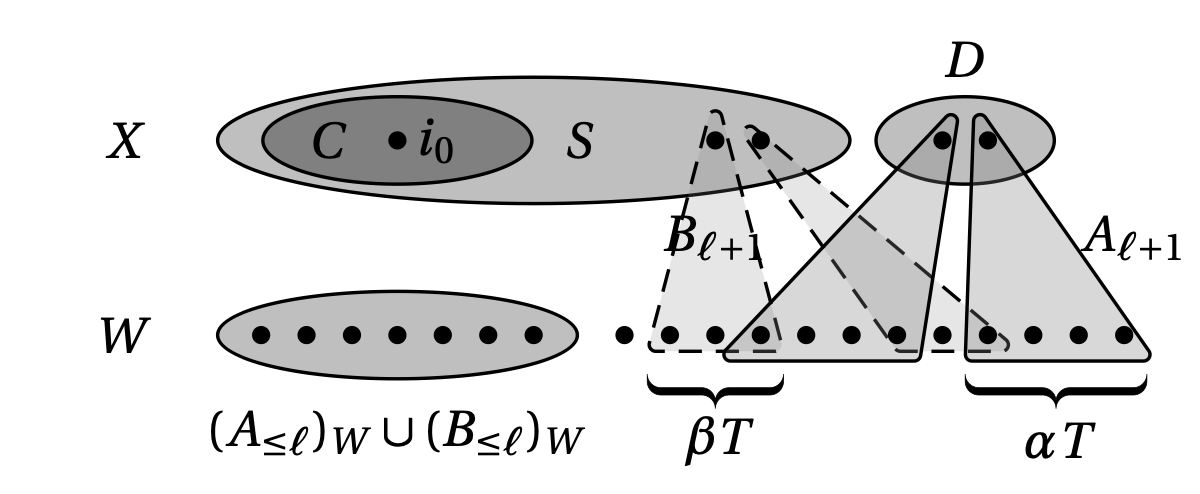
\includegraphics[width=10cm]{chapters/santaclaus/SC_fig2.png}
    \caption{Case 1 of the algorithm, 
    where a set $A_{\ell+1} \subseteq \pazocal{E}_{\alpha T}$ of hyperedges is found that intersects many new edges $
    B_{\ell+1} \subseteq (M \setminus B_{\leq \ell})$. In particular $|B_{\ell+1}| \geq \Omega_{\varepsilon}(|C|)$. 
    Note that $D$ might contain nodes from $C$.\label{fig:CaseIofTheAlgorithm}}
\end{center}
\end{figure}

\begin{figure}
    \begin{center}
        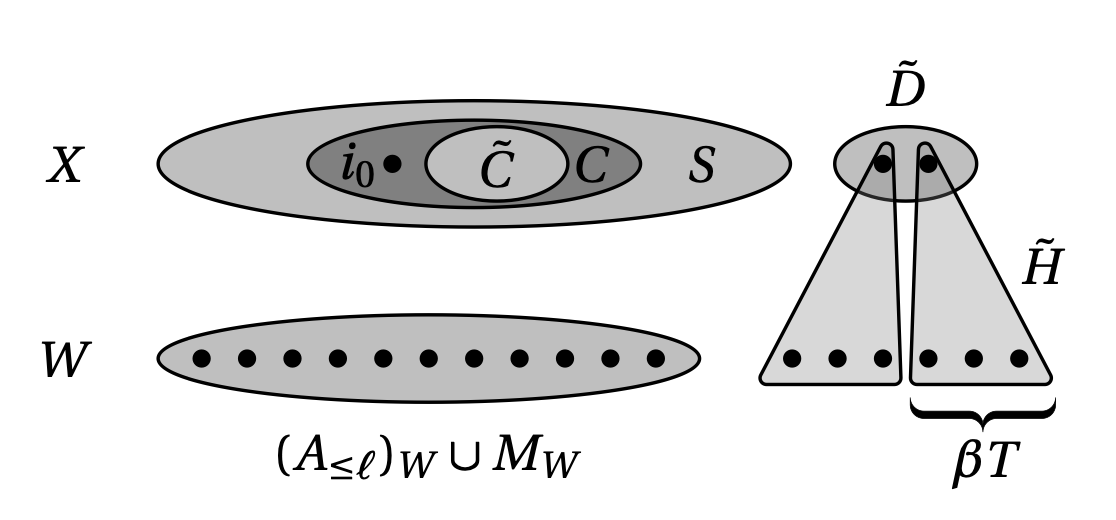
\includegraphics[width=10cm]{chapters/santaclaus/SC_fig3.png}
        \caption{Case 2 of the algorithm, 
        where $\tilde{H} \subseteq \pazocal{E}_{\beta T}$ of size $|\tilde{H}| \geq \Omega_{\varepsilon}(|C|)$ 
        is found so that $(i)$ $\tilde{H}$ is disjoint on the $W$-side to the matching $M$ and the adding edges in the augmenting tree, 
        $(ii)$ $\tilde{H}$ covers a set $\tilde{D}$ with $S \setminus \tilde{C} \cup \tilde{D} \in \pazocal{I}$, 
        and $(iii)$ $\tilde{C}$ is from one layer of the augmenting tree. 
        Here $\tilde{D}$ and $\tilde{C}$ do not have to be disjoint.\label{fig:CaseIIofTheAlgorithm}}
    \end{center}
    \end{figure}
% \begin{subfigure}{}
% \psset{xunit=0.7cm,yunit=0.5cm}
% \begin{pspicture}(-1,-2)(12,5)
% %\psset{linecolor=lightgray}
% %\psgrid[gridcolor=lightgray,subgridcolor=white](-2,-3)(12,5)
% \rput[c](0,3){$X$}
% \rput[c](0,0){$W$}
% %\psellipse(0,0)(1,1)
% \psellipse[linewidth=0.75pt,fillstyle=solid,fillcolor=lightgray](4.5,3)(3.5,1)\rput[c](5,3){$S$}% S
% \psellipse[linewidth=0.75pt,fillstyle=solid,fillcolor=gray](3,3)(1.5,0.7)\rput[c](2.25,3){$C$}% C
% \psellipse[linewidth=0.75pt,fillstyle=solid,fillcolor=lightgray](9.25,3)(1.0,0.7)\rput[c](9.25,4.25){$D$}% D
% \psellipse[linewidth=0.75pt,fillstyle=solid,fillcolor=lightgray](3,0)(2,0.7)\rput[c](3,-1.5){$(A_{\leq \ell})_W \cup (B_{\leq \ell})_W$}% A_W + B_
% % EDGES IN B_l+1
% %\pspolygon(6.5,3)(6,0)(7,0)
% \pspolygon[linearc=0.05,linewidth=0.75pt,linestyle=dashed,opacity=0.2,fillcolor=gray,fillstyle=solid](6.5,3.75)(5.75,-0.25)(7.25,-0.25)\rput[c](6.5,1.5){$B_{\ell+1}$}
% %\pspolygon(7.0,3)(8.5,0)(10,0)
% \pspolygon[linearc=0.05,linewidth=0.75pt,linestyle=dashed,opacity=0.2,fillcolor=gray,fillstyle=solid](6.5,3.7)(8.5,-0.25)(9.85,-0.25)
% % EDGES IN A_l+1
% %\pspolygon[linecolor=blue](9,3)(7,0)(8.5,0)
% \pspolygon[linearc=0.05,linewidth=0.75pt,linecolor=black,opacity=0.3,fillcolor=gray,fillstyle=solid](9.2,3.6)(6.5,-0.4)(8.75,-0.4)
% %\pspolygon[linecolor=blue](9.5,3)(9.5,0)(11,0)
% \pspolygon[linearc=0.05,linewidth=0.75pt,linecolor=black,opacity=0.3,fillcolor=gray,fillstyle=solid](9.35,3.6)(9.25,-0.4)(11.35,-0.4)\rput[l](10.5,1.5){$A_{\ell+1}$}
% % NODES IN X AND W
% \multido{\N=1.5+0.5}{7}{\cnode*(\N,0){2pt}{A}}
% \multido{\N=5.5+0.5}{12}{\cnode*(\N,0){2pt}{A}}
% \cnode*(3,3){2pt}{i0}\nput[labelsep=2pt]{0}{i0}{$i_0$}
% \cnode*(6.5,3){2pt}{B1}
% \cnode*(7.0,3){2pt}{B1}
% \cnode*(9.0,3){2pt}{A1}
% \cnode*(9.5,3){2pt}{A1}
% %\psbrace[rot=90,ref=1C,nodesepB=5pt](1,-1)(5,-1){$(A_{\leq \ell})_W \cup (B_{\leq \ell})_W$}
% \psbrace[rot=90,ref=1C,nodesepB=7pt,braceWidthInner=3pt,braceWidthOuter=3pt](5.75,-0.6)(7.25,-0.6){$\beta T$}
% \psbrace[rot=90,ref=1C,nodesepB=7pt,braceWidthInner=3pt,braceWidthOuter=3pt](9.25,-0.6)(11.25,-0.6){$\alpha T$}
% \end{pspicture}
% \caption{Case 1 of the algorithm, where a set $A_{\ell+1} \subseteq \pazocal{E}_{\alpha T}$ of hyperedges is found that intersects many new edges $B_{\ell+1} \subseteq (M \setminus B_{\leq \ell})$. In particular $|B_{\ell+1}| \geq \Omega_{\varepsilon}(|C|)$. Note that $D$ might contain nodes from $C$.\label{fig:CaseIofTheAlgorithm}}
% \end{subfigure}
% %\end{center}
% %\begin{center}
% \begin{subfigure}{}
% \psset{xunit=0.7cm,yunit=0.5cm}
% \begin{pspicture}(-1,-1.5)(12,5.5)
% %\psset{linecolor=lightgray}
% %\psgrid[gridcolor=lightgray,subgridcolor=white](-2,-3)(12,5)
% \rput[c](0,3){$X$}
% \rput[c](0,0){$W$}
% %\psellipse(0,0)(1,1)
% \psellipse[linewidth=0.75pt,fillstyle=solid,fillcolor=lightgray](4.5,3)(3.5,1)\rput[c](7.0,3){$S$}% S
% \psellipse[linewidth=0.75pt,fillstyle=solid,fillcolor=gray](4.5,3)(1.85,0.7)\rput[c](5.8,3){$C$}% C
% \psellipse[linewidth=0.75pt,fillstyle=solid,fillcolor=lightgray](4.75,3)(0.8,0.6)\rput[c](4.75,3){$\tilde{C}$}% \tilde{C}
% \psellipse[linewidth=0.75pt,fillstyle=solid,fillcolor=lightgray](9.25,3)(0.8,0.6)\rput[c](9.25,4.25){$\tilde{D}$}% D
% \psellipse[linewidth=0.75pt,fillstyle=solid,fillcolor=lightgray](4.0,0)(3,0.7)\rput[c](4,-1.5){$(A_{\leq \ell})_W \cup M_W$}% A_W + B_W
% % EDGES IN A_l+1)
% \pspolygon[linearc=0.05,linewidth=0.75pt,linecolor=black,opacity=0.3,fillcolor=gray,fillstyle=solid](9.1,3.6)(7.6,-0.4)(9.20,-0.4)
% \pspolygon[linearc=0.05,linewidth=0.75pt,linecolor=black,opacity=0.3,fillcolor=gray,fillstyle=solid](9.4,3.6)(9.30,-0.4)(10.90,-0.4)\rput[l](10.5,1.5){$\tilde{H}$}
% % NODES IN X AND W
% \multido{\N=1.5+0.5}{11}{\cnode*(\N,0){2pt}{A}}
% \multido{\N=8.00+0.50}{6}{\cnode*(\N,0){2pt}{A}}
% \cnode*(3.6,3){2pt}{i0}\nput[labelsep=1pt]{180}{i0}{$i_0$}
% \cnode*(9.0,3){2pt}{A1}
% \cnode*(9.5,3){2pt}{A2}
% %\psbrace[rot=90,ref=1C,nodesepB=5pt](1,-1)(5,-1){$(A_{\leq \ell})_W \cup (B_{\leq \ell})_W$
% \psbrace[rot=90,ref=1C,nodesepB=7pt,braceWidthInner=3pt,braceWidthOuter=3pt](9.30,-0.6)(10.90,-0.6){$\beta T$}
% \end{pspicture}
% \end{subfigure}
% \caption{Case 2 of the algorithm, where $\tilde{H} \subseteq \pazocal{E}_{\beta T}$ of size $|\tilde{H}| \geq \Omega_{\varepsilon}(|C|)$ is found so that $(i)$ $\tilde{H}$ is disjoint on the $W$-side to the matching $M$ and the adding edges in the augmenting tree, $(ii)$ $\tilde{H}$ covers a set $\tilde{D}$ with $S \setminus \tilde{C} \cup \tilde{D} \in \pazocal{I}$, and $(iii)$ $\tilde{C}$ is from one layer of the augmenting tree. Here $\tilde{D}$ and $\tilde{C}$ do not have to be disjoint.\label{fig:CaseIIofTheAlgorithm}}
% \end{center}
% \end{figure}


\subsection{Termination and runtime}



  As seen in Lemma~\ref{lem:ConstantSizeSwap}, 
\[
|X| \geq |B_{\leq \ell}|\geq \big(1+\frac{\varepsilon^2}{4} \big)^{\ell}|B_0|,
\]
and solving for $\ell$ shows $\frac{\log(|X|)}{\log \big(1+\frac{\varepsilon^2 }{4} \big)}  \geq \ell$.
Thus the total number of layers at any step in the algorithm is $O(\log|X|)$. 
Note after each collapse of the layers, the matching $M$ and possibly the independent set $S$ are updated. 
However, the fixed exposed node $i_0$ will remain in $S$ until the very last iteration in which the algorithm finds
an edge $e_1$ that augments the matching. 
Before we begin discussing the proof guaranteeing our algorithm terminates, we need a lemma to compare the number of blocking edges after a layer is collapsed to the number of blocking edges at the beginning of the iteration. 

\begin{lemma}\label{lem:ExtraSteps}
  Let $\tilde{\ell}$ be the index of the collapsed layer and let $B'$ be the updated blocking edges after a collapse step. Then,
  $|B'_{\leq \tilde{\ell}}| \leq |B_{\leq \tilde{\ell}}| \cdot (1- \frac{\varepsilon^2}{4} \cdot \gamma )$.
\end{lemma}
\begin{proof}
 Recall $B'_{\tilde{\ell}} = B_{\tilde{\ell}} \setminus F$ for $F$ the edges of $M$ covering $\tilde{C}$. Further, the blocking edges in layers indexed less than $\tilde{\ell}$ are not effected in the iteration. Hence
 \begin{eqnarray*}
  |B'_{\leq \tilde{\ell}}| &=& |B'_{\leq \tilde{\ell}-1}| + |B'_{ \tilde{\ell}}|=|B_{\leq \tilde{\ell}-1}| + |B'_{ \tilde{\ell}}| 
\end{eqnarray*}
From Lemmas~\ref{lem:GreedyMatchingExpansionLemma} and~\ref{lem:SizeOfOverlapOfNewEdgesWithM},
$|B_{\ell+1}| \geq \frac{\varepsilon^2}{4}|B_{\leq \ell}|$. Then examining the collapsed layer by itself, we see 
\begin{eqnarray*}
  |B'_{ \tilde{\ell}}| &=& |B_{ \tilde{\ell}}|-|F| \leq |B_{ \tilde{\ell}}| -   \frac{\varepsilon^2}{4} \cdot \gamma |B_{ \leq \tilde{\ell}}|.
\end{eqnarray*}
Substituting back into $|B'_{\leq \tilde{\ell}}|$, we find that
\begin{eqnarray*} 
  |B'_{\leq \tilde{\ell}}| &\leq& |B_{\leq \tilde{\ell}-1}| + |B_{ \tilde{\ell}}| -  \frac{\varepsilon^2}{4} \cdot \gamma |B_{ \leq \tilde{\ell}}| \\
  &=& |B_{\leq \tilde{\ell}}| - \frac{\varepsilon^2}{4} \cdot \gamma |B_{ \leq \tilde{\ell}}| =|B_{ \leq \tilde{\ell}}| 
  \cdot \big (1-\frac{\varepsilon^2}{4} \cdot \gamma \big).
\end{eqnarray*}
\end{proof}

To prove the algorithm terminates in polynomial time, we consider a signature vector $s = (s_0,s_1,\ldots, s_{\ell}, \infty)$, 
where $s_j = \lfloor \log_{c}|B_{\leq j}| \rfloor $ for $c = \frac{1}{1-\frac{\varepsilon^2 }{4}\cdot \gamma}$. 
The signature vector and proof that the algorithm terminates is inspired by \cite{AlgoForSantaClaus-AnnamalaiKalaitzisSvenssonSODA15}, 
but it is subtly different. 


\begin{lemma}\label{lem:LexOrderDecreases}
The signature vector decreases lexicographically after each iterative loop in the algorithm. 
\end{lemma}
\begin{proof}
Let $s = (s_0,\ldots,s_{\ell},\infty)$ be a signature vector at the beginning of a step in the algorithm, and let $s'$ be the result of $s$ through one iteration of the algorithm. For $\ell+1$ denoting the newest built layer in the algorithm, if the newest set of hyperedges found intersects at least $\frac{\varepsilon^2}{4}|C|$ many edges of $M$, then another layer in the augmenting tree is built and no layer is collapsed. Then $s' = (s_0,\ldots,s_{\ell},s_{\ell+1},\infty)$ is lexicographically smaller than $s$.

Otherwise, layer $0 \leq \tilde{\ell} \leq \ell$ is collapsed. All finite coordinates above $s_{\tilde{\ell}}$ are deleted from the signature vector, and all coordinates before $s_{\tilde{\ell}}$ are unaffected. So it suffices to check that $s'_{\tilde{\ell}} < s_{\tilde{\ell}}$. Again, let $B'$ be the updated blocking edges after a collapse step. As $B_{\tilde{\ell}}$ is the only set of blocking edges in $B_{\leq \tilde{\ell}}$ affected by the collapse, by Lemma~\ref{lem:ExtraSteps} one has $|B'_{\leq \tilde{\ell}}| \leq |B_{\leq \tilde{\ell}}|(1-\frac{\varepsilon^2}{4} \cdot \gamma )$. Taking a $\log$ we compare the coordinates
\[
s'_{\tilde{\ell}} = \left \lfloor \log_c \left ( \left |B'_{\leq \tilde{\ell}} \right | \right ) \right \rfloor \leq \left \lfloor \log_c \left ( \left |B_{\leq \tilde{\ell}} \right | \left (1- \frac{\varepsilon^2}{4} \cdot \gamma \right ) \right) \right \rfloor= 
\left \lfloor \log_c \left ( \left | B_{\leq \tilde{\ell}} \right | \right ) \right \rfloor -1 = s_{\tilde{\ell}}-1.
\]
\end{proof}
Choose the infinite coordinate to be some integer larger than $\log |X|$.  Since for every layer $\ell$, we have $|B_{\leq \ell}| \leq |X|$, then every coordinate of the signature vector is upper bounded by $U = O(\log |X|)$. Recall the number of layers, and thus the number of coordinates in the signature vector, is also upper bounded by $U$. Together, these imply that the sum of the coordinates of the signature vector is at most $U^2$. 

As the signature vector has non-decreasing order, each signature vector corresponds to a partition of an integer $z \leq U^2$. On the other hand, every partition of some $z \leq U^2$ has a corresponding signature vector. Thus we apply a result of Hardy and Ramanujan to find the total number of signature vectors is $\sum_{k \leq U^2} e^{O(\sqrt{k})} = |X|^{O(1)}$. Since each iteration of the algorithm can be done in polynomial time and the signature vector decreases lexicographically after each iteration, the algorithm terminates after a total time of $n^{\Theta_{\varepsilon}(1)}$. 

%\textbf{Theorem 5 to Thorem 2}- $|W|$ is different in the unit case than in the general case. To ensure this doesn't effect runtime, do we need to be more careful in splitting items than scaling everything so the smallest $p_j$ is 1, then breaking up the rest of the jobs into unit sizes? In particular, there's some assumption that $\{p_j\} \in \mathbb{Z}$ here. 



\section{Application to Santa Claus\label{sec:SantaClausApplication}}

In this section, we show a polynomial time $(4+\varepsilon)$-approximation algorithm
for the Santa Claus problem. Recall that 
for a given set of children $M$, and a set of presents $J$, the Santa Claus problem asks how Santa should distribute presents to children in order to maximize the minimum happiness of any child\footnote{We assume Santa to be an equitable man-- not one influenced by bribery, social status, etc.}.
Here, present $j$ is only wanted by some subset of children that we denote by $A_j \subseteq M$, and present $j$ has value $p_{j}$ to child $i \in A_j$. The happiness of child $i$ is the sum of all $p_{j}$ for presents $j$ assigned to child $i$. 
%We consider a restricted version of this problem where $p_{ij} \in\{0,p_j\}$, so $p_{ij}=0$ for all children $i$ such that $j \not \in A_i$ and otherwise children who want present $j$ all value it equally. 
We assume w.l.o.g. to know the integral objective function value $T$ of the optimum solution,
otherwise $T$ can be found by binary search.

We partition gifts into two sets: \emph{large} gifts $J_L := \{ j \in J \mid p_j > \delta_2 T\}$
and \emph{small} gifts $J_S := \{ j \in J \mid p_j \leq \delta_1 T\}$,
for parameters $0 < \delta_1 \leq \delta_2 < 1$ such that
% For fixed parameters $1 \geq \delta_2 \geq 1/4 > \delta_1 \geq 0$, where 
all gifts have values in $[0,\delta_1  T] \cup (\delta_2  T,T]$. 
Let $P(T,\delta_1,\delta_2)$ be the set of vectors $z \in \mathbb{R}_{\geq 0}^{J \times M}$ satisfying
\begin{eqnarray*}\label{eq:CompactLPforSC}
 \sum\limits_{j \in J_S: i \in A_j} p_j z_{ij} &\geq& T \cdot \Big( 1-\sum_{j \in J_L: i \in A_j} z_{ij}\Big)  \qquad \forall i \in M \\
  \sum\limits_{i \in A_j}z_{ij} &\leq& 1 \hspace{4.0cm} \forall j \in J \\
  z_{ij} &\leq& 1-\sum_{j' \in J_L: i \in A_{j'}} z_{ij'} \hspace{1.5cm} \forall j \in J_S \; \forall i \in A_j
\end{eqnarray*}

% \rem{S, Y: Should we be dropping unnecesary large jobs, or defining the basis of the matroid to be the machines forming the \textit{largest} matchings on $L$, not those forming $L$-perfect matchings}
If $n = |J| + |M|$, then this LP has $O(n^2)$ many variables and $O(n^2)$
many constraints. To see that this is indeed a relaxation, take any feasible assignment $\sigma : J \to M$ with $\sum_{j \in \sigma^{-1}(i)} p_j \geq T$ for all $i \in M$. 
Now let $\sigma : J \to M \cup \{ \emptyset \}$ be a modified 
assignment where we set $\sigma(j) = \emptyset$ for gifts that we decide to drop. For each child $i \in M$ that receives at least one large gift 
we drop all small gifts and all but one large gift. 
Then a feasible solution $z \in P(T,\delta_1,\delta_2)$ is obtained by letting  
\[ 
  z_{ij} := \begin{cases} 
 1 & \textrm{if }\sigma(j) = i \\
%1 & \textrm{if }\sigma(j) = i\textrm{ and }p_j \geq \delta \dot T  \\
%1 & \textrm{if }\sigma(j) = i\textrm{ and }p_j < \delta T\textrm{ and }\not\exists j'\textrm{ with } (\sigma(j')=i\textrm{ and }p_j' \geq \delta T)\\
0 & \textrm{otherwise}.
\end{cases}
\]


% The problem gives rise to the following linear program:


% \[\max \quad  T \]
% \[\sum\limits_{j \in J} p_{ij}x_{ij} \geq T \qquad \forall i \in M \]
% \[ \sum\limits_{i \in M} x_{ij} = 1 \qquad \forall j \in J \]
% \[ 0 \leq x_{ij} \leq 1 \qquad \forall i \in M, \forall j \in J,\]
% where $x_{ij}$ is the indicator variable for giving gift $j$ to child $i$. The first constraint ensures each child receives enough ``happiness'' and the second constraint ensures all gifts are assigned. 
% % This formulation has an unbounded integrality gap, as can be seen by considering the case when there are 2 machines which only admit jobs $j_1$ and $j_2$, where $p_{j_1} = 1$ and $p_{j_2}=T$ for large $T$. 


We will show that given a feasible solution $z \in P(T, \delta_1,\delta_2)$, there exists a feasible solution $(x^*,y^*)$ to $Q(T)$. To do this, we will exploit two underlying matroids in the Santa Claus problem, allowing us to apply Theorem~\ref{thm:MainMatroidAlgorithm}. Let 
\[
  \pazocal{I} = \left\{M_L \subseteq M |\; \exists \text{ left-perfect matching between } M_L\textrm{ and }J_L\textrm{ using edges }(i,j): i \in A_j\right\}, 
\]
be a family of independent sets. Then  $\pazocal{M} = (M,\pazocal{I})$ constitutes a \emph{matchable set matroid}.
% $\pazocal{M}$ obviously satisfies nonemptyness and monotonicity. For a proof that it satisfies the swapping condition, see section 10.3 in Schrijver's notes. 
%The bases of this matroid are 
%\[
%  \pazocal{B}(\pazocal{M}) = \{ M_L \subset M  | \quad \exists L \text{ perfect matching covering }M_L\}.
%\]
We denote the \emph{co-matroid} of $\pazocal{M}$ by $\pazocal{M}^* = (M, \pazocal{I}^*)$. Recall that the  independent sets 
of the co-matroid are given by
\[
  \pazocal{I}^* = \left\{M_S \subseteq M | \; \exists  M_L \in \pazocal{B}(\pazocal{M}):  M_S \cap M_L = \emptyset \right\}.
\]
% \[ \pazocal{B}(\pazocal{M}^*) = \{M_S \subset M | \quad M_S = M \setminus M_L \quad M_L \in \pazocal{B}(\pazocal{M}) \}
%\]


We can define a vector $x \in \setR^M$ with 
$ 
x_i = \sum_{j \in J_L: i \in A_j} z_{ij}
$
that lies in the matroid polytope of $\pazocal{M}$. This fact follows easily from the integrality of the fractional matching polytope in bipartite graphs. It is instructive to think of $x_i$ as the decision variable telling whether child $i \in M$ should receive a large present.

%For any $U \subseteq M$, $z(U)$ is the load between $U$ and large jobs admissable on $U$. As no node in this subgraph gives or receives load more than 1, $z(U)$ is upper bounded by the size of the minimum vertex cover, since otherwise some node in the minimum vertex cover would give or receive load more than 1. By K{\H o}nig's theorem, $z(U) \leq \textrm{rank}(U)$ with respect to the matchable set matroid.
Unfortunately, $x$ does not have to lie in the base polytope --- in fact the sum $\sum_{i \in M} x_i$ might not even be integral. 
%Given the existence of this vector $z$, using the following lemma, we find $z'$ in the base polytope of $\pazocal{M}$ where every machine is just as well covered with large jobs as in $z$.
However, there always exists a vector $x'$ in the base polytope that covers
every child just as well with large presents as $x$ does. 
%Recall the following fact from matroid theory: 
This observation can be stated for general matroids: 
\begin{lemma}\label{lem: RoundToBasePolytope}
Let $\pazocal{M} = (X,\pazocal{I})$ be any matroid and let $x$ be a point in its matroid polytope. Then in polynomial time one can find a point $x'$ in the base polytope so that $x' \geq x$ coordinate-wise. 
\end{lemma}
In fact the algorithm behind this claim is rather trivial: as long as $x \in P_{\pazocal{M}}$ is not in the base polytope, there is always a coordinate $i$ and a $\mu>0$ so that $x+\mu e_i \in P_{\pazocal{M}}$.

% \rem{Y: I changed $z+\delta e_i$ into $x+\delta e_i$, which should be just a typo.}

With the new vector $x' \in P_{\pazocal{B}(\pazocal{M})}$ at hand, we can redefine the $z$-assignments by letting
\[ 
  z_{ij}' = 
\begin{cases}
z_{ij} & \qquad x_i = 1\\ 
\frac{1-x_i'}{1-x_i} z_{ij} & \qquad x_i \neq 1.
\end{cases} 
\]
for $j \in J_S$; the new values $z_{ij}'$ for $j \in J_L$ can be obtained from the fractional matching
that corresponds to $x_i'$. Note that $0 \leq z_{ij}' \leq z_{ij}$ for $j \in J_S$. The reader should be convinced that
still $z' \in P(T,\delta_1,\delta_2)$, just that the corresponding vector $x'$ now lies in $P_{\pazocal{B}(\pazocal{M})}$\footnote{There is an alternative proof without the need to replace $x$ by $x'$. Add the constraint $\sum_{j \in J_L, i \in A_j} z_{ij} = \textrm{rank}(\pazocal{M})$
to $P(T,\delta_1, \delta_2)$. There is always a feasible integral solution satisfying this constraint. Then for any fractional solution $z \in P(T,\delta_1,\delta_2)$, the corresponding vector $x$ will immediately lie in the base polytope.}.

% \rem{Y: For the footnote, I am wondering if this change will make binary search difficult, since we need to define a matroid for each T.}

%Note that $y^*_{ij}$ is smaller than $y_{ij}$, as more machines are covered with large jobs. 
%With the overall goal of finding some pair feasible to $Q(T)$, we next observe that $x = 1-z'$ is in the base polytope of the comatroid $\pazocal{M}^*$.
It is well known in matroid theory that  
the complementary vector $x^* := \mathbb{1} - x'$ lies in $P_{\pazocal{B}(\pazocal{M}^*)}$. 
Again, it is instructive to think of $x^*_i$ as the decision variable whether 
child $i$ has to be satisfied with small gifts.
Finally, the assignments $y^*$ are simply the restriction of $z'$ on the 
coordinates $(i,j) \in M \times J_S$.
The obtained pair $(x^*,y^*)$ lies in $Q(T)$, where the matroid in the definition 
of $Q(T)$ is $\pazocal{M}^*$.
%\begin{lemma}\label{lem: ComplementBase}
%  Let $\pazocal{M} = (X,\pazocal{I})$ be any matroid and let $z$ be a point in the base polytope. Then one has that $1-z$ is in the base polytope of the comatroid of $\pazocal{M}$, $\pazocal{M}^*$.
%\end{lemma}

%The $x$ defined above is that which will be a part of the solution to $Q(T)$, and it remains to scale $y$ to find $y^*$. Restricting $y^*$ to the coordinates of $Q(T)$ and then substituting in $(x,y^*)$ for $Q(T)$, one sees it is a feasible solution.



% Let $G_{(T,\delta)} = (M \cup S, E_S)$ be the bipartite graph with $E_S$ the set of edges between children and small gifts, and let $N(i)$ denote the neighborhood of node $i$ in $E_S$ (to avoid $\delta$s with different meanings here).
% Now, we're able to rewrite $Q(T)$ as a linear program $P(T,\delta)$:
 

% \[\max \quad  T \]
% \[x \in P_{\pazocal{B}(\pazocal{M}^*_{(T,\delta)})}\]
% \[\sum\limits_{j \in N(i)} p_j y_{ij} \geq T \cdot x_i \qquad \forall i \in X\]
% \[ y(N(j)) \leq 1 \qquad \forall j \in S\]
% \[  y_{ij} \leq x_i \qquad \forall (i,j) \in E_S\]
% \[(x,y) \in \mathbb{R}_{\geq 0}^{M} \times \mathbb{R}_{\geq 0}^{E_S}\]


As $Q(T) \neq \emptyset$, we can apply Theorem~\ref{thm:MainMatroidAlgorithm} 
which results in a subset $M_S \in \pazocal{B}(\pazocal{M}^*) $
 of the children and an assignment $\sigma : J_S \to M_S$, 
where each child in $M_S$ receives happiness at least 
$ \big(\frac13 - \frac{\delta_1}{3} - \varepsilon \big) \cdot T$ from the assignment of small gifts.
Implicitly due to the choice of the matroid $\pazocal{M}^*$, 
we know that the remaining children $M \setminus M_S = M_L$ can all receive one large gift
and this assignment can be computed in polynomial time using a matching algorithm. 
Overall, each child receives either one large present of value
at least $\delta_2 \cdot T$ or small presents of total value at least $(\frac{1}{3} - \frac{\delta_1}{3}-\varepsilon ) \cdot T$. 
Therefore each child receives value at least
\begin{equation}\label{eq: balanceSC}
  \min\Big\{ \Big(\frac{1}{3}-\frac{\delta_1}{3}-\varepsilon\Big) \cdot T, \delta_2 \cdot T \Big\} \geq \Big(\frac{1}{4}-\varepsilon\Big) \cdot T
\end{equation}
for a choice of $\delta_2 = \delta_1=\frac{1}{4}$. 
In some instances of Santa Claus, we can do better. 
Set $\delta_1$ so that $\delta_1 \cdot T$ is the largest gift value
that is at most $\frac14 T$, and set $\delta_2$ so that $\delta_2 \cdot T$ 
is the smallest gift value that is at $\frac14 T$.
Then the algorithm guarantees that each child receives value at least 
as in the left hand side of Equation~\ref{eq: balanceSC}. 
When $\delta_1$ and $\delta_2$ are bounded away from $1/4$,
then the approximation improves. 
For example, when $\delta_2 \geq 1/3$ and $\delta_1 T$ is close to 0,
such as in the case where all gifts have value either $T$ or 1,
we approach a $(3+\varepsilon)$-approximation.

\section{Conclusion}
In this work, we introduced Matroid Max-Min Fair Allocation. 
for this problem, we construct a new, compact LP to model it, 
and we prove a $(3+\epsilon)$-approximation, modulo an additive term of $\frac13$ of the most valuable item's value $\frac13 \max_{w in W} p_w$.
Our algorithm is a local search based on Haxell's augmenting tree argument.
Overall, we can use our result on Matroid Max-Min Fair Allocation as a blackbox to obtain a $(4+\epsilon)$-approximation for Santa Claus.


One obvious, immediate open question is to resolve the gap between the lower bound of 2 and the upper bound of 4 for approximation Santa Claus.
We do not know the integrality gap for our LP, so it is unclear whether the LP can be used to obtain approximations better than 4. 
More broadly, this problem of Matroid Max-Min Fair Allocation might be useful to study other scheduling problems. 





%, which is in $\pazocal{B}(\pazocal{M})$ by definition of $\pazocal{B}(\pazocal{M}^*)$. In polynomial time, we can find a matching between $M_L$ and $L$. Thus we have an assignment that assigns each child either one large gift, and thus happiness at least $\delta \cdot T$, or enough small gifts to have happiness at least $(\frac13 - \varepsilon - \delta) \cdot T$. A choice of $\delta \approx \frac16$ maximizes all children's happiness.




%In particular this sets $y_{ij} = 0$ for small jobs that are unnecessary because $i$ already receives a large job.


\chapter{Scheduling with Communication Delays on Identical Machines}\label{chapter: S1}
\section{Introduction}

Scheduling jobs with precedence constraints is a fundamental problem in approximation algorithms and combinatorial optimization.
In this problem we are given $m$ identical  machines and a set  $J$ of $n$ jobs, where each job $j$ has a processing length $p_j  \in \mathbb{Z}_+$.
The jobs have precedence constraints, which are given by a partial order $\prec$. 
A constraint $j \prec j'$ encodes that job $j'$ can only start after job $j$ is completed.
The goal is to find a schedule of jobs that minimizes {\em makespan}, which is the completion time of the last job.
This problem is denoted\footnote{
	Throughout the paper we use the standard scheduling three-field notation~\cite{GLLR79,VeltmanLL90}.
	The respective fields
	denote:
	\textbf{(1)
	number of identical machines:} $\p \infty$: unlimited; $\p$: number $m$ of machines given as input; $\p m$: constant number $m$ of machines,
	\textbf{(2) job properties:} $\Prec$: precedence constraints; $p_j=1$: unit-size jobs; $c$:~communication delays of length $c$ (can be $c_{jk}$ if dependent on jobs $j \prec k$); $\Intervals$: see Section~\ref{sec:approximation_for_pinfty}; $\dup$: allowed duplication of jobs,
	\textbf{(3) objective:} $\Cmax$: minimize makespan; $\wjcj$: minimize weighted sum of completion times.
%	\end{itemize}%
}
by $\p \mid \Prec \mid \Cmax$.
In a seminal result from 1966, Graham ~\cite{GrahamListScheduling1966} showed that the greedy list scheduling algorithm achieves a $\left(2- \frac{1}{m}\right)$-approximation. 
%The algorithm simply  computes an arbitrary topological ordering of the jobs, and whenever a machine becomes idle selects the first
%available job from the list. 
By now, our understanding of the approximability of this basic problem is almost complete: 
it had been known since the late `70s, due to a result by Lenstra and Rinnooy Kan~\cite{LR78}, that it is NP-hard to obtain better than $4/3$-approximation, and in 2010 Svensson~\cite{Svensson10} showed that, assuming a variant of the Unique Games Conjecture~\cite{BansalK10}, it is NP-hard to get a $(2-\varepsilon)$-approximation for any $\varepsilon > 0$.

The above precedence-constrained scheduling problem models the task of distributing workloads onto multiple processors or servers, which is ubiquitous in computing.
This basic setting takes the dependencies between work units into account, but not the data transfer costs between machines, which is critical in applications. 
A precedence constraint $j \prec j'$ typically implies that the input to $j'$ depends on the output of $j$.
In many real-world scenarios, especially in the context of scheduling in data centers, if $j$ and $j'$ are executed on different machines, then the {\em communication delay} due to transferring this output to the other machine cannot be ignored.
This is an active area of research in applied data center scheduling literature, where several new abstractions have been proposed to deal with communication delays~\cite{Chowdhury, guo2012spotting,hong2012finishing,shymyrbay2018meeting,zhang2012optimizing,zhao2015rapier,luo2016towards}.
 Another timely example is found in the parallelization of Deep Neural Network training
(the machines being accelerator devices such as GPUs, TPUs, or FPGAs).
There, when training the network on one sample/minibatch per device in parallel, the communication costs incurred by synchronizing the weight updates in fact dominate the overall running time~\cite{narayanan2018pipedream}.
Taking these costs into account,
it turns out that
it is better to split the network onto multiple devices, forming a ``model-parallel'' computation pipeline~\cite{huang2019gpipe}.
In the resulting \emph{device placement} problem,
the optimal split crucially depends on the communication costs
between dependent layers/operators.


\medskip

A classic model that captures the effect of data transfer latency on scheduling decisions is the problem of {\em scheduling jobs with precedence and communication delay constraints}, introduced by Rayward-Smith~\cite{RAYWARDSMITH1987} and Papadimitriou and Yannakakis~\cite{PapadimitriouY90}.
The setting, denoted by $\p \mid \Prec, c \mid \Cmax$, is similar to the makespan minimization problem described earlier, except for one crucial difference.
Here  we are  given a {\em communication delay parameter} $c \in  \setZ_{\ge 0}$, and the output schedule must satisfy the property that if $j \prec j'$ and $j$, $j'$ are scheduled on {different machines}, then $j'$ can only start executing at least $c$ time units after $j$ had finished. 
On the other hand,  if $j$ and $j'$ are scheduled on the {same machine}, then $j'$ can start executing immediately after $j$ finishes. 
In a closely related problem, denoted by $\p \infty \mid \Prec, c \mid \Cmax$, a schedule can use as many machines as desired.
The goal is to schedule jobs {\em non-preemptively} so as to minimize the makespan.  In a non-preemptive schedule, each job $j$ needs to be  assigned to a single machine and executed during $p_j$ consecutive timeslots.
The problems $\p \mid \Prec, c \mid \Cmax$ and $\p \infty \mid \Prec, c \mid \Cmax$ are the focus of this paper.

Despite its theoretical significance and practical relevance, very little is known about the communication delay setting.
A direct application of Graham's~\cite{GrahamListScheduling1966} list scheduling algorithm yields a $(c+2)$-approximation,
and no better algorithm is known for the problem.
Over the years, the problem has attracted significant attention, but all known results,
which we discuss below in Section~\ref{sec:related_work}, concern special settings, small communication delays, or hardness of approximation. 
To put this in perspective, we note that the current best algorithm for general~$c$~\cite{GiroudeauKMP08}, which achieves an approximation factor of $2/3 \cdot (c+1)$, only marginally improves on Graham's algorithm while requiring the additional assumptions that the number of machines is unbounded and $p_j = 1$.
This is in sharp contrast to the basic problem  $\p \mid \Prec \mid \Cmax$ (which would correspond to the case $c=0$), where the approximability of the problem is completely settled under a variant of the Unique Games Conjecture.
This situation hints that incorporating communication delays in scheduling  decisions requires fundamentally new algorithmic ideas compared to the no-delay setting.
Schuurman and Woeginger~\cite{SW99a} placed the quest for getting better algorithms to the problem in their influential list of top-10 open problems in scheduling theory.
In a recent MAPSP 2017 survey talk,  Bansal~\cite{Bansalmapsp} highlighted the lack of progress on this model, describing it as ``not understood at all; almost completely open'', and suggested that this is due to the lack of promising LP/SDP relaxations.


\subsection{Our Contributions}

The main result of this paper is the following:

\begin{theorem} \label{thm:main_sched1}
There is a randomized $O(\log c \cdot \log m)$-approximation algorithm for $\p \mid \Prec, c \mid \Cmax$ with expected polynomial running time, where $c, p_j \in \setN$.
\end{theorem}

In any non-preemptive schedule the number $m$ of machines is at most the number $n$ of jobs, so for the easier $\p \infty$ version of the problem, the above theorem implies the following:

\begin{corollary} \label{cor:colmain_sched1}
There is a randomized $O(\log c \cdot \log n)$-approximation algorithm for $\p \infty \mid \Prec, c \mid \Cmax$ with expected polynomial running time, where $c, p_j \in \setN$.
\end{corollary}

For both problems one can replace either $c$ or $m$ by $n$, yielding a $O(\log^2 n)$-approximation algorithm.
Our results make substantial progress towards resolving  one of the questions in ``Open Problem 3'' in the survey of Schuurman and Woeginger~\cite{SW99a}, which asks whether a constant-factor approximation algorithm exists for $\p \infty \mid \Prec, c \mid \Cmax$.

Our approach is based on a Sherali-Adams lift of a time-indexed linear programming relaxation for the problem, followed by a randomized clustering of the semimetric space induced by this lift.
It is possible to write a more compact LP for the problem for which our algorithm and analysis still work. 
However, as we will show in Section~\ref{sec:IntegralityGap}, this compact LP has integrality gap $ \Omega(\sqrt{\log n})$.
%To our knowledge, it is the first application of clustering in metric spaces to scheduling problems.
To our knowledge, this is the first instance of a multiple-machine scheduling problem being viewed via the lens of metric space clustering.
We believe that our framework is fairly general and should extend to other problems involving scheduling with communication delays.
To demonstrate the broader applicability of our approach, we also consider the objective of minimizing the weighted sum of completion times. Here each job $j$ has a weight $w_j$, and the goal is to minimize $\sum_{j} w_j C_j$, where $C_j$ is the completion time of $j$.  

\begin{theorem} \label{thm:maincomp_sched1}
There is a randomized $O(\log c \cdot \log n)$-approximation algorithm for  $\p \infty \mid \Prec, p_j = 1, c \mid \sum_{j} w_j C_j$ with expected polynomial running time, where $c \in \setN$.
\end{theorem}

No non-trivial approximation ratio was known for this problem prior to our work. 



\subsection{Independent work of Maiti {\em et al}}
In a parallel and independent work, Maiti {et al.}~\cite{MRSSV} developed an $O(\log^2 n \log^2 m \log c / \log \log c)$-approximation algorithm for the makespan objective function on {\em related machines} ($Q \mid \Prec, c \mid \Cmax$).
Interestingly, they obtained the results using completely different techniques compared to ours.
While our results are based on LP hierarchies and clustering, Maiti {et al.}~\cite{MRSSV} developed a novel framework based on {\em job duplication}.
In their framework, they first construct a schedule where a single job can be scheduled on {\em multiple machines}, which is known to effectively ``hide'' the communication delay constraints \cite{PapadimitriouY90}.
Quite surprisingly, Maiti {et al.}~\cite{MRSSV} showed that one can convert a schedule with duplication to a feasible schedule without duplication, where every job is processed on a single machine, while increasing the makespan by at most an $O(\log^2 n \log m)$ factor.
 Maiti {et al.} also prove an integrality gap for the LP they consider, which is different than ours. However, after seeing their result, we found that their integrality gap instance works for a compact form of our LP as well, which we prove in Section~\ref{sec:IntegralityGap}.


\subsection{Our Techniques}



As we alluded earlier, there is a lack of
combinatorial lower bounds for scheduling with communication delays. For example, consider {Graham's list scheduling algorithm}, which greedily processes jobs on $m$ machines as soon as they become available. One can revisit the analysis of Graham~\cite{GrahamListScheduling1966} and show that there exists a chain $Q$ of dependent jobs such that the makespan achieved by list scheduling is bounded by

\[
  \frac{1}{m} \sum_{j \in J} p_j + \sum_{j \in Q} p_j + c \cdot (|Q|-1). 
\]
The first two terms are each lower bounds on the optimum --- the 3rd term is not. In particular, it is unclear 
how to certify that the optimal makespan is high because of the communication delays. However, this argument suffices for a
$(c+2)$-approximation, since $p_j \geq 1$ for all $j \in J$.

As pointed out by Bansal~\cite{Bansalmapsp}, there is no known promising LP relaxation. To understand the issue
let us consider the special case $\p \infty \mid \Prec, p_j=1, c \mid \Cmax$. Extending, for example, the LP of Munier and K\"onig~\cite{MunierKonig}, one might choose
variables $C_j$ as completion times, as well as decision variables $x_{j_1,j_2}$ denoting whether $j_2$ is executed in the time window $[C_{j_1},C_{j_1}+c)$ on the same machine as $j_1$. Then we can try to enforce communication delays by requiring that $C_{j_2} \geq C_{j_1} + 1 + (c-1) \cdot (1-x_{j_1,j_2})$ for $j_1 \prec j_2$. Further, we enforce load constraints $\sum_{j_1 \in J} x_{j_1,j_2} \leq c$ for $j_2 \in J$ and $\sum_{j_2 \in J} x_{j_1,j_2} \leq c$ for $j_1 \in J$. To see why this LP fails, note that in any instance where the maximum dependence degree is bounded by $c$, one could simply set $x_{j_1,j_2} = 1$ and completely avoid paying any communication delay.
Moreover, this problem seems to persist when moving to more complicated LPs that incorporate indices for time and machines.
%, the hope arises that this is indeed a \emph{local consistency issue}$
%rather than a global one.

A convenient observation is that, in exchange for a constant-factor loss in the approximation guarantee, it suffices to
find an assignment of jobs to length-$c$ intervals such that dependent jobs scheduled in the same length-$c$ interval must be
assigned to the same machine.
(The latter condition will be enough to satisfy the communication delay constraints
as, intuitively, between every two length-$c$ intervals we will insert an empty one.)
In order to obtain a stronger LP relaxation, we consider an \emph{$O(1)$-round Sherali-Adams lift} of an inital LP with indices for time and machines. %In  which is slightly non-standard as we have mix of binary and continuous decision variables.
%the underlying LP which in our setting
%can still be done with a bit of care, even though we have a mix of binary continuous decision variables.
From the lifted LP, we extract a \emph{distance function} $d: J \times J \to [0,1]$ which satisfies the following properties: 
\begin{enumerate}
\item[(i)] The function $d$ is a \emph{semimetric}.
\item[(ii)] $C_{j_1} +  d(j_1,j_2) \leq C_{j_2}$ for $j_1 \prec j_2$.
\item[(iii)] Any set $U \subseteq J$ with a diameter of at most $\frac{1}{2}$ w.r.t. $d$, satisfies $|U| \leq 2c$.
\end{enumerate}
%with the following properties: 
Here we have changed the interpretation of $C_j$ to the \emph{index} of the length-$c$ interval in which $j$ will be processed.
Intuitively, $d(j_1,j_2)$ can be understood as the probability that jobs $j_1,j_2$ are \emph{not} being scheduled within the same length-$c$ interval on the same machine. To see why a constant number of Sherali-Adams rounds are helpful, observe that the triangle inequality behind $(i)$ is really a property depending only on \emph{triples} $\{ j_1,j_2,j_3\}$ of jobs and an $O(1)$-round Sherali-Adams lift
would be locally consistent for every triple of variables.

We will now outline how to round such an LP solution. 
For jobs whose LP completion times are sufficiently different, say $C_{j_1} + \Theta(\frac{1}{\log(n)}) \leq C_{j_2}$,
we can afford to deterministically schedule $j_1$ and $j_2$ at least $c$ time units apart while only paying a $O(\log n)$-factor more than the LP. Hence the critical case is to sequence a set of jobs $J^* = \{ j \in J \mid C^* \leq C_j \leq C^* + \Theta(\frac{1}{\log(n)}) \}$
whose LP completion times are very close to each other. Note that by property $(ii)$, we know that any dependent jobs $j_1,j_2 \in J^*$ must have $d(j_1,j_2) \leq \Theta(\frac{1}{\log(n)})$.
As $d$ is a semimetric, we can make use of the rich toolset from the theory of metric spaces. 
In particular, we use an algorithm by Calinescu, Karloff and Rabani~\cite{DBLP:journals/siamcomp/CalinescuKR04}: 
For a parameter $\Delta>0$, one can partition a semimetric space into \emph{random clusters} so that the
diameter of every cluster is bounded by $\Delta$ and each $\delta$-neighborhood around a node is separated, 
meaning contains jobs assigned to different clusters, 
with probability at most  $O(\log(n)) \cdot \frac{\delta}{\Delta}$.
Setting $\delta := \Theta(\frac{1}{\log(n)})$ and $\Delta := \Theta(1)$ one can then show that a fixed job $j \in J^*$ will be
in the same cluster as \emph{all} its ancestors in $J^*$ with probability at least $\frac{1}{2}$, while all clusters have diameter at most $\frac{1}{2}$. By $(iii)$, each cluster will contain at most $2c$ many (unit-length) jobs, and consequently we can schedule all the clusters in parallel, where we drop any job that got separated from any ancestor.
Repeating the sampling $O(\log n)$ times then schedules all jobs in $J^*$. This reasoning results in a $O(\log^2 n)$-approximation
for this problem, which we call $\p \infty \mid \Prec, p_j=1, \Intervals \mid \Cmax$. With a bit of care the approximation factor can be improved to $O(\log c \cdot \log m)$.

Finally, the promised $O(\log c \cdot \log m)$-approximation for the more general problem $\p \mid \Prec, c \mid \Cmax$
follows from a reduction to the described special case $\p \infty \mid \Prec, p_j=1, \Intervals \mid \Cmax$.
%Finally we give a reduction that implies the same approximation factor for



\subsection{History of the Problem} \label{sec:related_work}

Precedence-constrained scheduling problems of minimizing the makespan and sum of completion times objectives have been extensively studied  for many decades in various settings. We refer the reader to~\cite{michael2018scheduling,lawler1993sequencing,PruhsST04,ambuhl2008precedence,svensson2009approximability} for more details.
Below, we only discuss results directly related  to the communication delay problem in the offline setting.


\paragraph{Approximation algorithms.}
As mentioned earlier,  Graham's~\cite{GrahamListScheduling1966} list scheduling algorithm
yields a $(c+2)$-approximation
for
$\p \mid \Prec, c \mid \Cmax$,
and a $(c+1)$-approximation for the $\p \infty$ variant.
For unit-size jobs and $c \ge 2$,
Giroudeau, K\"onig, Moulai and Palaysi~\cite{GiroudeauKMP08}
improved the latter
($\p \infty \mid \Prec, p_j=1, c \ge 2 \mid \Cmax$)
to a $\frac{2}{3}(c+1)$-approximation.
For unit-size jobs and $c = 1$,
Munier and K\"onig~\cite{MunierKonig}
obtained a $4/3$-approximation
via LP rounding % favorite successor
($\p \infty \mid \Prec, p_j=1, c=1 \mid \Cmax$);
for the $\p$ variant,
Hanen and Munier~\cite{HanenMunier73Apx}
gave an easy reduction from the $\p \infty$ variant
that loses an additive term of $1$ in the approximation ratio,
thus yielding a $7/3$-approximation.
Thurimella and Yesha~\cite{ThurimellaYesha}
gave a reduction that,
given an $\alpha$-approximation algorithm for $\p \infty \mid \Prec, c, p_j=1 \mid \Cmax$,
would yield a $(1 + 2 \alpha)$-approximation algorithm for $\p \mid \Prec, c, p_j=1 \mid \Cmax$.


For a constant number of machines,
a hierarchy-based approach of Levey and Rothvoss~\cite{LeveyR16} for the no-delay setting
($\p m \mid \Prec, p_j=1 \mid \Cmax$)
was 
generalized by Kulkarni, Li, Tarnawski and Ye~\cite{KulkarniLTY20}
to allow for communication delays that are also bounded by a constant.
For any $\varepsilon > 0$ and $\hat c \in \setZ_{\ge 0}$,
they give a nearly quasi-polynomial-time $(1+\varepsilon)$-approximation algorithm
for $\p m \mid \Prec, p_j=1, c_{jk} \le \hat c \mid \Cmax$.
The result also applies to arbitrary job sizes, under the assumption that preemption of jobs is allowed, but migration is not.

\iffalse
\subsection{Hierarchies in Scheduling}
One can take a  linear programming relaxation for any optimization problem that has a large integrality gap, 
and strengthen it automatically by applying an LP or SDP hierarchy lift. 
While this principle has been known since a long time, there are very few results in scheduling algorithms  where hierarchies have helped obtaining better algorithms. 
\fi

\paragraph{Hardness.}
Hoogeveen, Lenstra and Veltman~\cite{HoogeveenLV94} showed that even the special case $\p \infty \mid \Prec, p_j=1, c=1 \mid \Cmax$ is NP-hard to approximate to a factor  better than $7/6$.
For the case with bounded number of machines (the $\p$~variant)
%setting $\p \mid \Prec, p_j=1, c=1 \mid \Cmax$ (the number of processors being part of the input)
they show $5/4$-hardness.
These two results can be generalized for $c \ge 2$ to $(1+1/(c+4))$-hardness~\cite{GiroudeauKMP08}
and $(1+1/(c+3))$-hardness~\cite{BampisGK96},
respectively.% (the latter holds also for the $\dup$ version).
\footnote{
	Papadimitriou and Yannakakis~\cite{PapadimitriouY90} claim a $2$-hardness for
	%the no-duplication version
	$\p \infty \mid \Prec, p_j=1, c \mid \Cmax$,
	but give no proof.
	Schuurman and Woeginger~\cite{SW99a} remark that ``it would be nice to have a proof for this claim''.
}


\paragraph{Duplication model.}
The communication delay problem has also been studied (to a lesser extent) in a setting where jobs can be duplicated (replicated), i.e., executed on more than one machine, in order to avoid communication delays.
%As an example, consider an instance with $n-1$ machines, $n$ unit-size jobs with precedence constraints $1 \prec 2$, $1 \prec 3$, $1 \prec 4$, ..., $1 \prec n$, and $c = n$. The optimal makespan without duplication  is $n$, but using duplication one can get makespan $2$
%(begin by executing job $1$ on every machine).
This assumption seems to significantly simplify the problem,
especially when we are also given an unbounded number of machines:
already in 1990,
Papadimitriou and Yannakakis~\cite{PapadimitriouY90} gave a rather simple $2$-approximation algorithm for $\p \infty \mid \Prec, p_j, c_{jk}, \dup \mid \Cmax$.
Observe that this result holds even when communication delays are unrelated (they depend on the pair of jobs).
%Colin and Chr\'etienne~\cite{ColinC91}
%gave an exact algorithm
%for the case
%$\p \infty \mid \Prec, c_{jk}, \dup, \max c_{jk} \le \min p_j \mid \Cmax$,
%where processing times are arbitrary,
%but communication delays are smaller than processing times.
%Jung, Kirousis and Spirakis~\cite{JungKS93}
%gave an exact algorithm
%based on dynamic programming
%for $\p \infty \mid \Prec, p_j=1, c, \dup \mid \Cmax$
%that runs in time $O(n^{c+1})$.
%Munier and Hanen~\cite{HanenMunierDuplication}
%gave a $2$-approximation\footnote{We ignore lower-order terms such as $-1/m$.}
%for $\p \mid \Prec, p_j=1, c=1, \dup \mid \Cmax$.
The only non-trivial approximation algorithm for arbitrary $c$ and a bounded number of machines is due to Lepere and Rapine~\cite{LepereR02}, who gave an asymptotic $O(\log c / \log \log c)$-approximation for $\p \mid \Prec, p_j=1, c, \dup \mid \Cmax$.
On the hardness side,
Papadimitriou and Yannakakis~\cite{PapadimitriouY90}
showed NP-hardness of
$\p \infty \mid \Prec, p_j=1, c, \dup \mid \Cmax$
(using a large delay $c = \Theta(n^{2/3})$).

%Besides being seemingly easier to approximate,
%we also believe that the replication model is less applicable in most real-world scenarios due to the computation and energy cost of replication, as well as because replication is more difficult to achieve if the computations are nondeterministic in some sense (e.g.~randomized).

\bigskip
\noindent
Many further references can be found in~\cite{VeltmanLL90,GiroudeauKMP08,Drozdowski09,GiroudeauKoenig07,ColinC91,JungKS93,HanenMunierDuplication}.






















\section{Preliminaries}\label{sec: prelims_scheduling}


\subsection{The Sherali-Adams Hierarchy for LPs with Assignment Constraints}

In this section, we review the \emph{Sherali-Adams hierarchy} which provides an automatic strengthening of
linear relaxations for 0/1 optimization problems.
The authorative reference is certainly Laurent~\cite{Comparison-of-Hierarchies-Laurent-MOR03},
and we adapt the notation from Friggstad et al.~\cite{LP-for-DST-FriggstadKKLST-IPCO14}.
Consider a set of variable indices $[n] = \{ 1,\ldots,n\}$ and let $U_1,\ldots,U_N \subseteq [n]$
be subsets of variable indices.
We consider a polytope
\[
  K = \Big\{ x \in \setR^n \mid \tilde{A}x \geq \tilde{b}, \;\; \sum_{i \in U_k} x_i = 1 \;\; \forall k \in [N], \;\; 0 \leq x_i \leq 1 \;\; \forall i \in [n] \Big\},
\]
which we also write in a more compact form as $K = \{ x \in \setR^n \mid Ax \geq b\}$ with $A \in \setR^{m \times n}$ and $b \in \setR^m$.
We note that we included  explicitly the ``box constraints'' $0 \leq x_i \leq 1$ for all variables $i$.
Moreover, the constraint matrix contains \emph{assignment constraints} of the form $\sum_{i \in U_k} x_i = 1$.
This is the aspect that is non-standard in our presentation.

The general goal is to obtain a strong relaxation for the integer hull $\textrm{conv}( K \cap \{ 0,1\}^n)$.
Observe that any point $x \in \textrm{conv}( K \cap \{ 0,1\}^n)$ can be interpreted as a \emph{probability distribution} $X$ over points $K \cap \{ 0,1\}^n$. We know that any distribution can be described by the $2^n$ many values
$y_{I} = \Pr[\bigwedge_{i \in I}(X_i=1)]$ for $I \subseteq [n]$ --- in fact, the probability of any other event can be reconstructed
using the \emph{inclusion-exclusion formula}, for example $\Pr[X_1=1\textrm{ and }X_2=0] = y_{\{1\}}-y_{\{1,2\}}$.
While this is an exact approach, it is also an inefficient one.
In order to obtain a polynomial-size LP, we only work with variables $y_I$ where $|I| \leq O(1)$. 
Hence, for $r \geq 0$, we denote $\pazocal{P}_r([n]) := \{ S \subseteq [n] \mid |S| \leq r\}$ as all the index sets of size at most $r$.

\begin{definition}
  Let $SA_r(K)$ be the set of vectors $y \in \setR^{\pazocal{P}_{r+1}([n])}$ satisfying $y_{\emptyset} = 1$ and
  \[
 \sum_{H \subseteq J} (-1)^{|H|} \cdot \Big(\sum_{i=1}^n A_{\ell,i}y_{I \cup H \cup \{ i\}} - b_{\ell}y_{I \cup H}\Big) \geq 0 \quad \forall \ell \in [m]
\]
for all $I,J \subseteq [n]$ with $|I| + |J| \leq r$.
\end{definition}
The parameter $r$ in the definition is usually called the \emph{rank} or \emph{number of rounds} of the Sherali-Adams
lift.
It might be helpful for the reader to verify that for $I=J=\emptyset$, the constraint simplifies to $\sum_{i=1}^n A_{\ell,i}y_{\{ i\}} \geq b_{\ell}y_{\emptyset}=b_{\ell}$,
which implies that $(y_{\{1\}},\ldots,y_{\{n\}}) \in K$. Moreover it is instructive to verify that for any feasible integral solution  $x \in K \cap \{ 0,1\}^n$ one can set
$y_{I} := \prod_{i \in I} x_i$ to obtain a vector $y \in SA_r(K)$.



\begin{theorem}[Properties of Sherali-Adams] \label{thm:PropertiesOfSA}
  Let $y \in SA_r(K)$ for some $r \geq 0$. Then the following holds: 
  \begin{enumerate}
  \item[(a)] For $J \in \pazocal{P}_r([n])$ with $y_{J} > 0$, the vector $\tilde{y} \in \setR^{\pazocal{P}_{r+1-|J|}([n])}$ defined by $\tilde{y}_{I} := \frac{y_{I \cup J}}{y_J}$ satisfies $\tilde{y} \in SA_{r-|J|}(K)$.
  \item[(b)] One has $0 \leq y_{I} \leq y_J \leq 1$ for $J \subseteq I$ and $|I| \leq r+1$.
  \item[(c)] If $|J| \leq r+1$ and $y_i \in \{ 0,1\} \; \forall i \in J$, then $y_I = y_{I \setminus J} \cdot \prod_{i \in I \cap J} y_i$ for all $|I| \leq r+1$.
  \item[(d)] For $J \subseteq [n]$ with $|J| \leq r$ there exists a distribution over vectors $\tilde{y}$ such that $(i)$ $\tilde{y} \in SA_{r-|J|}(K)$, (ii) $\tilde{y}_i \in \{ 0,1\}$ for $i \in J$, (iii) $y_I = \E[\tilde{y}_I]$ for all $I \subseteq [n]$ with $|I \cup J| \leq r+1$ (this includes in particular all $I \in \pazocal{P}_{r+1-|J|}([n])$).
    \item[(e)] For $I \subseteq [n]$ with $|I| \leq r$ and $k \in [N]$ one has $y_I = \sum_{i \in U_k}y_{I \cup \{i\}}$.
  \item[(f)] Take $H \subseteq [N]$ with $|H| \leq r$ and set $J := \bigcup_{k \in H} U_k$. Then there exists a distribution over vectors $\tilde{y}$ such that (i) $\tilde{y} \in SA_{r-|H|}(K)$, (ii) $\tilde{y}_i \in \{ 0,1\}$ for $i \in J$, (iii) $y_I = \E[\tilde{y}_I]$ for all $I \in \pazocal{P}_{r+1-|H|}([n])$.
  \end{enumerate}
  
\end{theorem}
\begin{proof}
  For (a)-(d), we refer to the extensive coverage in Laurent~\cite{Comparison-of-Hierarchies-Laurent-MOR03}. We prove (e) and (f) which are non-standard and custom-tailored to LPs with assignment constraints: 
  \begin{enumerate}
  \item [(e)] Fix $I \subseteq [n]$ with $|I| \leq r$. We apply (d) to obtain a distribution over $\tilde{y}$ with $\tilde{y} \in SA_{r-|I|}(K)$ so that $\tilde{y}_i \in \{ 0,1\}$ for $i \in I$. Then
    \[
\sum_{i \in U_k} y_{I \cup \{ i\}}\stackrel{\textrm{linearity}}{=} \E\Big[ \sum_{i \in U_k} \tilde{y}_{I \cup \{ i\}}\Big] \stackrel{(c)}{=} \E\Big[ \tilde{y}_I \cdot \underbrace{\sum_{i \in U_k} \tilde{y}_i}_{=1}\Big] = \E[\tilde{y}_I] = y_I.
    \]
Here we apply $(c)$ for index sets $I \cup \{ i\}$ where variables in $J := I$ have been made integral. Note that indeed $|I \cup (I \cup \{ i\})| \leq r+1$ as required. 
\item[(f)] By an inductive argument it suffices to consider the case of $|H| = 1$.
  Let $H = \{ k\}$ and set $U := U_k$, i.e. the constraints for polytope $P$ contain the assignment constraint $\sum_{i \in U} x_i = 1$ and we want to make all variables
  in $U$ integral while only losing a \emph{single} round in the hierarchy. Abbreviate $U^+ := \{ i \in U \mid y_{\{i\}} > 0\}$.
  For $i \in U^+$, define $y^{(i)} \in \setR^{\pazocal{P}_{r}([n])}$
  to be the vector with $y^{(i)}_I := \frac{y_{I \cup \{ i\}}}{y_i}$. By (a) we know that $y^{(i)} \in SA_{r-1}(K)$. Moreover $y^{(i)}_{\{i\}} = \frac{y_{\{i\}}}{y_{\{i\}}} = 1$. Then the assignment constraint of the LP forces that $y_{\{i'\}}^{(i)} = 0$ for $i' \in U \setminus \{ i\}$. Now we define a probability distribution over vectors
  $\tilde{y}$ as follows: for $i \in U^+$, with probability $y_i$ we set $\tilde{y} := y^{(i)}$. Then (i) and (ii) hold for $\tilde{y}$  as discussed.
  Property (iii) follows from
  \[
\E[\tilde{y}_I] = \sum_{i \in U^+} y_i y_I^{(i)} = \sum_{i \in U^+} y_i \frac{y_{I \cup \{i\}}}{y_i} = \sum_{i \in U^+} y_{I \cup \{i\}} \stackrel{(b)}{=} \sum_{i \in U} y_{I \cup \{ i\}} \stackrel{(e)}{=} y_I
  \]
 \end{enumerate} 
\end{proof}
It is known that Theorem~\ref{thm:PropertiesOfSA}.(f) holds in a stronger form for the SDP-based \emph{Lasserre hierarchy}.
 Karlin, Mathieu and Nguyen~\cite{Hierarchies-for-Knapsack-KarlinMathieuNguyen-IPCO11} proved a result that can be paraphrased as follows:
  \emph{if one has any set $J \subseteq [n]$ of variables with the property that
there is no LP solution with more than $k$ ones in $J$, then one can make all variables of $J$ integral while losing only $k$ rounds}.
Interestingly, Karlin, Mathieu and Nguyen prove that this is completely false for Sherali-Adams. 
In particular, for a Knapsack instance with unit size items and capacity $2-\varepsilon$, 
the integrality gap is still $2-2\varepsilon$ after $\Theta_{\varepsilon}(n)$ rounds of Sherali-Adams.
In a different setting, Friggstad et al.~\cite{LP-for-DST-FriggstadKKLST-IPCO14}
realized that given a ``tree constraint'', a Sherali-Adams lift can provide
the same guarantees that Rothvoss~\cite{DirectedSteinerTreeAndLasserre-RothvossArxiv2011} derived from Lasserre. 
While Friggstad et al.~did not state their insight in the generality that we need here, our Lemma~\ref{thm:PropertiesOfSA}.(e)+(f) are inspired by their work.


\subsection{Semimetric Spaces}
\label{sec:semimetric spaces}

A \emph{semimetric space} is a pair $(V,d)$ where $V$ is a finite set (we denote $n := |V|$)
and $d : V \times V \to \setR_{\geq 0}$ is a \emph{semimetric}, i.e.
\begin{itemize}
\item $d(u,u) = 0$ for all $u \in U$.
\item Symmetry: $d(u,v) = d(v,u)$ for all $u,v \in V$.
\item Triangle inequality: $d(u,v) + d(v,w) \geq d(u,w)$ for all $u,v,w \in V$. 
\end{itemize}
Recall that the more common notion is that of a \emph{metric}, which additionally requires
that $d(u,v) > 0$ for $u \neq v$.
For a set $U \subseteq V$ we denote the \emph{diameter} as $\textrm{diam}(U) := \max_{u,v \in U} d(u,v)$. 
Our goal is to find a partition $V = V_1 \dot{\cup} \ldots \dot{\cup} V_k$ such that the diameter
of every cluster $V_i$ is bounded by some parameter $\Delta$.
We denote $d(w,U) := \min\{ d(w,u) : u \in U\}$ as the distance to the set $U$.
Moreover, for $r \geq 0$ and $U \subseteq V$, let $N(U,r) := \{ v \in V \mid d(v,U) \leq r\}$ 
be the \emph{distance $r$-neighborhood} of $U$.

We use a very influential clustering algorithm due to
Calinescu, Karloff and Rabani~\cite{DBLP:journals/siamcomp/CalinescuKR04},
which assigns each $v \in V$ to a random cluster center $c \in V$ such that $d(u,c) \leq \beta \Delta$.
Nodes assigned to the same cluster center form one block $V_i$ in the partition. 
Formally the algorithm is as follows:
\begin{center}
 \fbox{
\begin{minipage}{14cm}
\textsc{CKR Clustering algorithm} \vspace{2mm} \hrule \vspace{1mm}
{\bf Input:} Semimetric space $(V,d)$ with  $V = \{ v_1,\ldots,v_n\}$, parameter $\Delta>0$ \\
{\bf Output:} Clustering $V = V_1 \dot{\cup} \ldots \dot{\cup} V_k$ for some $k$. \vspace{1mm} \hrule \vspace{1mm}
\begin{enumerate*}\label{alg: CKR}
\item[(1)] Pick a uniform random $\beta \in [\frac{1}{4},\frac{1}{2}]$
\item[(2)] Pick a random ordering $\pi : V \to \{ 1,\ldots,n\}$ 
\item[(3)] For each $v \in V$ set $\sigma(v) := v_{\ell}$ so that $d(v,v_{\ell}) \leq \beta \cdot \Delta$ and $\pi(v_\ell)$ is minimal 
\item[(4)] Denote the points $v \in V$ with $\sigma^{-1}(v) \neq \emptyset$ by $c_1,\ldots,c_k \in V$ and return clusters $V_i := \sigma^{-1}(c_i)$ for $i=1,\ldots,k$
\end{enumerate*}
\end{minipage}}
\end{center}


Note that the algorithm has two sources of randomness: it picks a random parameter $\beta$,
and independently it picks a random ordering $\pi$. Here the ordering is to be understood such that 
element $v_{\ell}$ with $\pi(v_{\ell}) = 1$ is the ``highest priority'' element. 
%We will state and reprove
%the analysis of the CKR Clustering Algorithm with a slight generalization from pairs (i.e. $|U|=2$) to the
%separation of a general node set.
The original work of Calinescu, Karloff and Rabani~\cite{DBLP:journals/siamcomp/CalinescuKR04} only provided an upper bound on the probability that a short edge $(u,v)$ is separated. Mendel and Naor~\cite{RamseyPartitions-MendelNaorFOCS06} note that the same clustering provides the guarantee of
$\Pr[N(u,t)\textrm{ separated}] \leq 1 - O(\frac{t}{\Delta} \cdot \ln( \frac{|N(u,\Delta)|}{|N(u,\Delta/8)|}))$
for all $u \in V$ and $0\leq t<\frac{\Delta}{8}$.
% where $B(u,t) := \{ v \in V \mid d(u,v) \leq t\}$ is the radius-$t$ ball around $u$ in the space.
Mendel and Naor attribute this
to Fakcharoenphol, Rao and Talwar~\cite{TreeMetricFakcharoenpholRaoTalwar-JCSS04} (while Fakcharoenphol, Rao and Talwar\cite{TreeMetricFakcharoenpholRaoTalwar-JCSS04} do not state it explicitly in this form and focus on the ``local growth ratio'' aspect).
Instead of the algorithm by Calinescu, Karloff and Rabani~\cite{DBLP:journals/siamcomp/CalinescuKR04},
one could also cluster using the techniques of Leighton and Rao~\cite{RegionGrowing-LeightonRao-JACM1999} or those of Garg, Vazirani and Yannakakis \cite{Garg93approximatemax-flow}.
%However it is not hard to observe that a minor modification of the analysis also upperbounds the probability for a low-diameter set to be separated.
%The statement that we require is implied by Remark 3.1. in Mendel and Naor~? who attribute the statement to \footnote{The paper of FKR }
% We will show the following properties of the CKR Clustering Algorithm.
% . by Calinescu, Karloff and Rabani.
We state the formal claim in a form that will be convenient for us.
\begin{theorem}[Analysis of CKR] \label{thm:ProbUSeperatedByClustering}
  Let $V = V_1 \dot{\cup} \ldots \dot{\cup} V_k$ be the random partition of the CKR algorithm. The following holds:
  \begin{enumerate*}
  \item[(a)] The blocks have $\textrm{diam}(V_i) \leq \Delta$ for $i=1,\ldots,k$.
  \item[(b)] Let $U \subseteq V$ be a subset of points. Then \vspace{-2mm}
  \[
  \Pr[U\textrm{ is separated by clustering}] \leq \ln\big(2\big|N\big(U,\Delta/2 \big)\big|\big) \cdot \frac{4\textrm{diam}(U)}{\Delta} \leq \ln(2n) \cdot \frac{4\textrm{diam}(U)}{\Delta}.
\]
\end{enumerate*}
\end{theorem}
In the above, \emph{separated} means that there is more than one index $i$ with $V_i \cap U \neq \emptyset$.
\begin{proof}
The claim from (a) is easy to show as
\[
\textrm{diam}(V_i) = \max_{u,v \in V_i} d(u,v) \leq 2\max_{u \in V_i} \underbrace{d(u,c_i)}_{\leq \beta \Delta} \leq \Delta
\]
The tricky part is to show part (b).
The following definition and lemma are needed.
\begin{definition}
  Let us say that a node $w$ is a \emph{separator} for $U$, if
  \begin{enumerate*}
  \item[(A)] $\sigma(u) = w$ for at least one $u \in U$
  \item[(B)] $\sigma(u) \neq w$ for at least one $u \in U$
  \end{enumerate*}
  Moreover, if the set of separators of $U$ is non-empty, then we call the separator
  that comes first in the order $\pi$ the \emph{first separator}.
\end{definition}


Next, we show that nodes that are closer to the set $U$ are the most likely to be the first separator: 
\begin{lemma} \label{lem:CKR-ProbWsIsFirstSeparator}
  Let $w_1,\ldots,w_n$ be the nodes sorted so that $d(w_1,U) \leq \ldots \leq d(w_n,U)$.
  Then \\$\Pr[w_s\textrm{ is the first separator for }U] \leq \frac{4}{s} \cdot \frac{\textrm{diam}(U)}{\Delta}$.
\end{lemma}
\begin{proof}
  Let $u_{\min} := \textrm{argmin}\{ d(u,w_s) : u \in U\}$ and $u_{\max} := \textrm{argmax}\{ d(u,w_s) : u \in U\}$
  be the closest and furthest point from $w_s$.
%   \begin{figure}
%   \begin{center}
%   \ifrenderfigures
%     \begin{pspicture}(0,0)(6,3)
%       \psellipse[linestyle=dashed](4.8,1.4)(1.45,0.8) \rput[r](3.6,2){$U$}
%      \cnode*(0,0){2.5pt}{w5} \nput{-90}{w5}{$w_s$}
%      \cnode*(1,0){2.5pt}{w4} \nput{-90}{w4}{$w_{s-1}$}
%      \cnode*(3,0){2.5pt}{w3}
%      \cnode*(4,0){2.5pt}{w2} \nput{-90}{w2}{$w_2$}
%      \cnode*(5,0){2.5pt}{w1} \nput{-90}{w1}{$w_1$}
%      \rput[c](2,0){$\ldots$}
%      \cnode*(5,0.8){2.5pt}{u1}
%      \cnode*(3.8,1){2.5pt}{u2} % \nput{-90}{w5}{$w_s$}
%      \cnode*(6,1.5){2.5pt}{u3}
%      \cnode*(5,2){2.5pt}{u4}
%      \ncline{<->}{u2}{u3} \naput[labelsep=0pt]{$\leq \textrm{diam}(U)$}
%      \nput{180}{u2}{$u_{\min}$}
%      \nput{0}{u3}{$u_{\max}$}
%    \end{pspicture}
%    \fi
%  \end{center}
%  \caption{Visualization of CKR analysis}
% \end{figure}
  We claim that in order for $w_s$ to be the first separator, both of the following
  conditions must hold:
\begin{enumerate*}
\item[(i)] $d(w_s,u_{\min}) \leq \beta \cdot \Delta < d(w_s,u_{\max})$
\item[(ii)] The order selects $w_s$ as the first node among $w_1,\ldots,w_s$.
\end{enumerate*}
We assume that $w_s$ is the first separator, and
suppose for the sake of contradiction that either (i) or (ii) (or both) are not satisfied.
We verify the cases:
\begin{itemize}
\item \emph{Case: $\beta \Delta < d(w_s,u_{\min})$.} Then no point will be assigned to $w_s$ and $w_s$ is not a separator at all.
\item \emph{Case: $\beta \Delta \geq d(w_s,u_{\max})$.} As $w_s$ is a separator, there are nodes $u_1,u_2 \in U$
  with $\sigma(u_1) = w_s$ and $\sigma(u_2) \neq w_s$. Then $\sigma(u_2)$ has to come earlier in the order $\pi$ as $d(w_s,u_2) \leq \beta \Delta$. Hence $w_s$ is not the first separator.
\item \emph{Case: $w_s$ is not first among $w_1,\ldots,w_s$ with respect to $\pi$.} By assumption there
  is an index $1 \leq s_2 <s$ such that $\pi(w_{s_2}) < \pi(w_s)$. As $w_s$ is a separator, there
  is a $u_1 \in U$ with $\sigma(u_1) = w_s$.
  Let $u_2 := \textrm{argmin}\{ d(u,w_{s_2}) : u \in U\}$ be the point in the set $U$ that is closest to $w_{s_2}$.
  Then $d(u_2,w_{s_2}) = d(w_{s_2},U) \leq d(w_s,U) \leq d(w_s,u_1) \leq \beta \Delta$. 
  Hence $u_2$ would be assigned to a point of order at most $\pi(w_{s'}) < \pi(w_s)$, and therefore $w_s$ is not the first separator.
\end{itemize}
Now we estimate the probability that $w_s$ is the first separator.
 The parameter $\beta$ and the permutation are chosen independently, so $(i)$ and $(ii)$ are
independent events. Clearly $\Pr[(ii)] = \frac{1}{s}$. Moreover
\[
  \Pr[(i)] = \frac{|[d(w_s,u_{\min}),d(w_s,u_{\max})] \cap [\frac{\Delta}{4},\frac{\Delta}{2}]|}{\Delta/4}
  \leq \frac{4d(u_{\min},u_{\max})}{\Delta} \leq \frac{4\textrm{diam}(U)}{\Delta},
\]
where we have used the triangle inequality and the notation  $|[a,b]| = b-a$ for the length of an interval.
\end{proof}
Now we can finish the proof of Theorem~\ref{thm:ProbUSeperatedByClustering}:
\begin{proof}[Proof of Theorem~\ref{thm:ProbUSeperatedByClustering}]
  As in Lemma~\ref{lem:CKR-ProbWsIsFirstSeparator}, let $w_1,\ldots,w_n$ be an order of nodes such that $d(w_1,U) \leq \ldots \leq d(w_n,U)$.
  Note that $L := |N(U,\frac{\Delta}{2})| \leq n$ is the maximal index with $d(w_L,U) \leq \frac{\Delta}{2}$.
  If $U$ is separated, then there has to be a first separator.
Therefore, the following holds:
  \begin{eqnarray*}
    \Pr[U\textrm{ is separated}] &\leq& \sum_{s=1}^L \Pr[w_s\textrm{ is first separator for }U] \\
    &\stackrel{\textrm{Lem~\ref{lem:CKR-ProbWsIsFirstSeparator}}}{\leq}& \underbrace{\sum_{s=1}^L \frac{1}{s} \cdot}_{\leq \ln(2L)} \frac{4\textrm{diam}(U)}{\Delta} \leq \ln(2L) \cdot \frac{4\textrm{diam}(U)}{\Delta}
  \end{eqnarray*}
  Here we use that $\Pr[w_s\textrm{ is first separator for }U] = 0$ for $s>L$ since a node $w_s$ that has a distance bigger than $\frac{\Delta}{2}$ to $U$ will never be a separator.
\end{proof}
\end{proof}




%There are metric spaces (e.g. take $d(i,j) := |i-j|$ with $V = \{ 1,\ldots,n\}$) where any partition will separate two points that are close.
%To overcome this,
%we use a random partition, so that close points only have a
%a small probability of being separated.








\section{Approximation for  $\p \infty \mid \Prec, p_j=1, \Intervals \mid C_{\max}$}
\label{sec:approximation_for_pinfty}

In this section, we provide an approximation algorithm for scheduling $n$ unit-length jobs $J$ with
communication delay $c \in \setN$ on an unbounded number of machines so that precedence constraints given
by a partial order $\prec$ are satisfied. Instead of working with  $\p \infty \mid \Prec, p_j=1, c \mid C_{\max}$ directly, it will be
more convenient to consider a slight variant that we call $\p \infty \mid \Prec, p_j=1, \Intervals \mid C_{\max}$.
This problem variant has the same input but the time horizon is partitioned into time {\em intervals} of length $c$,
say $I_s = [sc, (s+1)c)$ for $s \in \setZ_{\geq 0}$.
The goal is to assign jobs to intervals and machines. % so that precedence constraints are preserved.
We require that if $j_1 \prec j_2$
then either $j_1$ is scheduled in an earlier interval than $j_2$ or $j_1$ and $j_2$ are scheduled in the same
interval on the same machine. Other than that, there are no further communication delays.
The objective function is to minimize the number of intervals used to process the jobs.
In fact we do not need to decide the order of jobs within intervals as any topological order will work.
In a more mathematical notation, the problem asks to find a partition $J = \dot{\bigcup}_{s \in \{0,\ldots,S-1\},i \in \setN} J_{s,i}$
with $|J_{s,i}| \leq c$ such that $S$ is minimized and for every $j_1 \prec j_2$ with $j_1 \in J_{s_1,i_1}$ and  $j_2 \in J_{s_2,i_2}$
one has either $s_1<s_2$ or $(s_1,i_1)=(s_2,i_2)$.
%as we can simply allow idle time $c$ between intervals.
See Figure~\ref{fig:ExamplePinftyIntervals} for an illustration.

It is rather straightforward to give reductions between $\p \infty \mid \Prec, p_j=1, c \mid C_{\max}$ and $\p \infty \mid \Prec, p_j=1, \Intervals \mid C_{\max}$ that only lose a small constant factor in both directions. The only subtle point to consider here
is that when the optimum makespan for $\p \infty \mid \Prec, c \mid C_{\max}$ is less than $c$, the problem admits a PTAS;
we refer to Section~\ref{sec:Reductions} for details. 


\begin{figure}
\begin{center}
    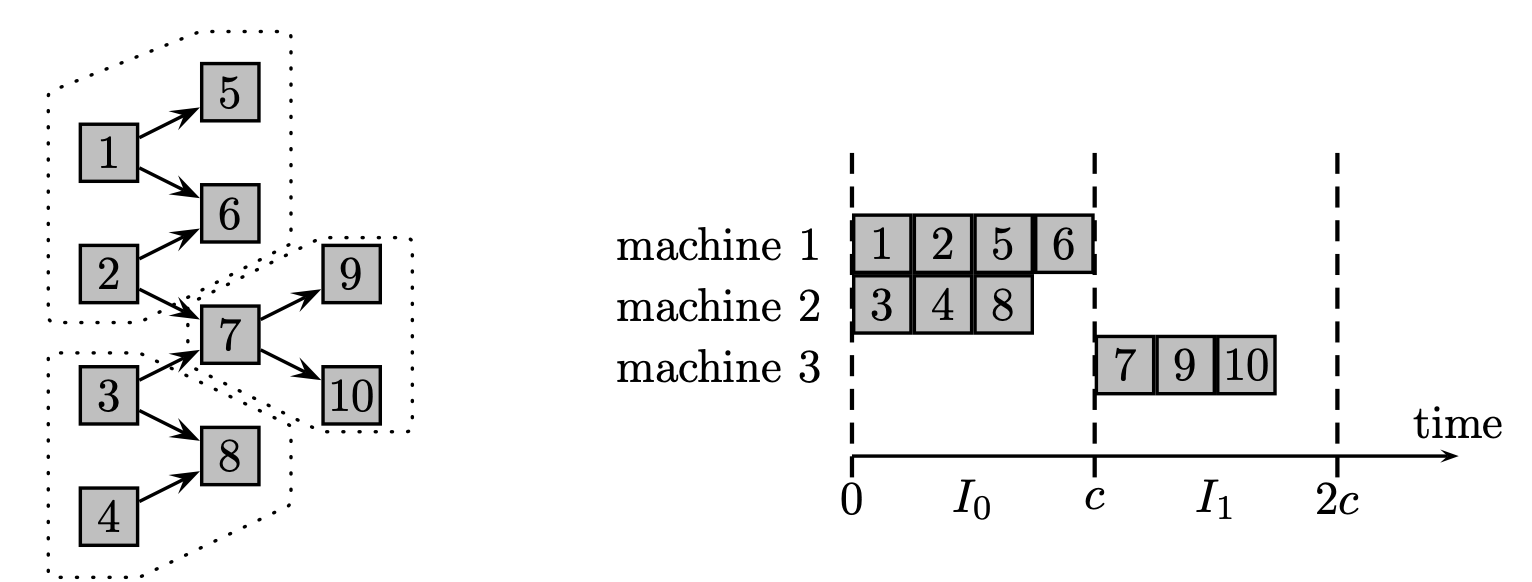
\includegraphics[width=15cm]{chapters/scheduling1/scheduling_intervals.png}
%   \psset{unit=0.5cm}
%   \begin{pspicture}(0,0)(6,6)
%   %  \psaxes(0,0)(-1,-1)(5,7)
%     \pspolygon[linestyle=dotted,linearc=0.1](-1,3.2)(0.5,3.2)(3,4.5)(3,8)(1.5,8)(-1,7)
%     \pspolygon[linestyle=dotted,linearc=0.1](-1,-1)(-1,2.7)(0.5,2.7)(3,1.5)(3,0.2)(0.5,-1)
%     \pspolygon[linestyle=dotted,linearc=0.1](1.3,2.5)(1.3,3.5)(3.5,4.6)(5,4.6)(5,1.4)(3.5,1.4)
%     \fnode[framesize=1,fillcolor=lightgray,fillstyle=solid](0,6){j1}\rput[c](j1){$1$}
%     \fnode[framesize=1,fillcolor=lightgray,fillstyle=solid](0,4){j2}\rput[c](j2){$2$}
%     \fnode[framesize=1,fillcolor=lightgray,fillstyle=solid](0,2){j3}\rput[c](j3){$3$}
%     \fnode[framesize=1,fillcolor=lightgray,fillstyle=solid](0,0){j4}\rput[c](j4){$4$}
%     \fnode[framesize=1,fillcolor=lightgray,fillstyle=solid](2,7){j5}\rput[c](j5){$5$}
%     \fnode[framesize=1,fillcolor=lightgray,fillstyle=solid](2,5){j6}\rput[c](j6){$6$}
%     \fnode[framesize=1,fillcolor=lightgray,fillstyle=solid](2,3){j7}\rput[c](j7){$7$}
%     \fnode[framesize=1,fillcolor=lightgray,fillstyle=solid](2,1){j8}\rput[c](j8){$8$}
%     \fnode[framesize=1,fillcolor=lightgray,fillstyle=solid](4,4){j9}\rput[c](j9){$9$}
%     \fnode[framesize=1,fillcolor=lightgray,fillstyle=solid](4,2){j10}\rput[c](j10){$10$}
%     \ncline[arrowsize=5pt]{->}{j1}{j5}
%     \ncline[arrowsize=5pt]{->}{j1}{j6}
%     \ncline[arrowsize=5pt]{->}{j2}{j6}
%     \ncline[arrowsize=5pt]{->}{j2}{j7}
%     \ncline[arrowsize=5pt]{->}{j3}{j7}
%     \ncline[arrowsize=5pt]{->}{j3}{j8}
%     \ncline[arrowsize=5pt]{->}{j4}{j8}
%     \ncline[arrowsize=5pt]{->}{j7}{j9}
%     \ncline[arrowsize=5pt]{->}{j7}{j10}
%   \end{pspicture}
%   \begin{pspicture}(-6,-1)(10,4)
%     \fnode[framesize=1,fillcolor=lightgray,fillstyle=solid](0.5,3.5){j1}\rput[c](j1){$1$}
%     \fnode[framesize=1,fillcolor=lightgray,fillstyle=solid](1.5,3.5){j2}\rput[c](j2){$2$}
%     \fnode[framesize=1,fillcolor=lightgray,fillstyle=solid](2.5,3.5){j5}\rput[c](j5){$5$}
%     \fnode[framesize=1,fillcolor=lightgray,fillstyle=solid](3.5,3.5){j6}\rput[c](j6){$6$}
%     \fnode[framesize=1,fillcolor=lightgray,fillstyle=solid](0.5,2.5){j3}\rput[c](j3){$3$}
%     \fnode[framesize=1,fillcolor=lightgray,fillstyle=solid](1.5,2.5){j4}\rput[c](j4){$4$}
%     \fnode[framesize=1,fillcolor=lightgray,fillstyle=solid](2.5,2.5){j8}\rput[c](j8){$8$}
%     \fnode[framesize=1,fillcolor=lightgray,fillstyle=solid](4.5,1.5){j7}\rput[c](j7){$7$}
%     \fnode[framesize=1,fillcolor=lightgray,fillstyle=solid](5.5,1.5){j9}\rput[c](j9){$9$}
%      \fnode[framesize=1,fillcolor=lightgray,fillstyle=solid](6.5,1.5){j10}\rput[c](j10){$10$}
%     \psline[linewidth=1pt,linestyle=dashed](0,-5pt)(0,5)
%     \psline[linewidth=1pt,linestyle=dashed](4,-5pt)(4,5)
%     \psline[linewidth=1pt,linestyle=dashed](8,-5pt)(8,5)
%     \psline{->}(0,0)(10,0) \rput[c](10,8pt){time}
%     \rput[r](-0.5,3.5){machine 1}
%     \rput[r](-0.5,2.5){machine 2}
%     \rput[r](-0.5,1.5){machine 3}
%     \rput[c](0,-10pt){$0$}
%     \rput[c](4,-10pt){$c$}
%     \rput[c](8,-10pt){$2c$}
%     \rput[c](2,-10pt){$I_0$}
%     \rput[c](6,-10pt){$I_1$}
%   \end{pspicture}
\caption{Left: example of an instance of $\p \infty \mid \Prec, p_j=1, \Intervals \mid C_{\max}$ with $c=4$ (where the partial order $\prec$ is the transitive closure of the depicted digraph). Right: a valid schedule in 2 intervals.\label{fig:ExamplePinftyIntervals}}  
\end{center}
\end{figure}
%In the next section, we give a reduction from $\p m \mid \Prec \mid \Cmax$ to this special case $P\infty \mid \Prec, p_j=1, c\textrm{-intervals} \mid C_{\max}$ losing only $O(1)$-factor  in the approximation ratio.



\subsection{The Linear Program}

Let $m \in \setN$ be a parameter defining the number of machines that we admit for the LP.  
Moreover, let $S \in \setN$ be the number of intervals that we allow for the time horizon.
To obtain an approximation for $\p \infty \mid \Prec, p_j=1, \Intervals \mid C_{\max}$  one can set $m := n$ and perform a binary
search to find the minimal $S$ for which the LP is feasible. But we prefer to keep the approach general.

%By doing  binary search, we can assume that an optimal solution to a given instance can be scheduled using at most $S$ intervals.
We construct the LP in two steps. % for $P\infty \mid \Prec, p_j=1, c\textrm{-intervals} \mid C_{\max}$ in two steps. 
First consider the variables
\[
  x_{j,i,s} = \begin{cases} 1 & \textrm{if }j\textrm{ is scheduled on machine }i\textrm{ in interval }I_s \\ 0 & \textrm{otherwise} \end{cases} \quad \forall j \in J, i \in [m], s \in \{ 0,\ldots,S-1\}
%  \theta_j = index of interval where j is scheduled 
\]
Let $K$ be the set of fractional solutions to the following linear system
\begin{eqnarray*}
  \sum_{i \in [m]} \sum_{s \geq 0} x_{j,i,s} &=& 1 \quad \forall j \in J \\
  \sum_{j \in J} x_{j,i,s} &\leq& c \quad \forall i \in [m] \;\; \forall s \in \{ 0,\ldots,S-1\} \\
%  \sum_{s'\leq s} \sum_{i \in [m]} x_{j_1,i,s'} &\geq& \sum_{s' \leq s} \sum_{i \in [m]} x_{j_2,i,s'} \quad \forall j_1 \prec j_2 \;\; \forall s \in \{ 0,\ldots,S-1\} \\
  0 \leq x_{j,i,s} &\leq& 1 \quad \forall j \in J, i \in [m], s \in \{ 0,\ldots,S-1\}
\end{eqnarray*}
So far, $K$ simply assigns jobs (fractionally) to intervals and machines without taking any precedence  constraints into account. %is consists  assignment 
%The LP asks for a (fractional) schedule where for a pair $j_1 \prec j_2$, $j_2$ cannot be scheduled in an earlier interval.
%However, it does not enforce that $j_1$ and $j_2$ be performed in separate intervals if they are not scheduled on the same machine.
Next, we will use a lift $x \in \textsc{SA}_r(K)$ containing variables
$x_{(j_1,i_1,s_1),(j_2,i_2,s_2)}$, which provide the probability for the event that $j_1$ is scheduled in interval $s_1$ on machine $i_1$ and
$j_2$ is scheduled in interval $s_2$ on machine $i_2$. We introduce two more types of decision variables: 
\begin{eqnarray*}
  y_{j_1,j_2} &=& \begin{cases} 1 & j_1\textrm{ and }j_2\textrm{ are scheduled on the same machine in the same interval} \\ 0 & \textrm{otherwise} \end{cases} \\
   C_j &=& \textrm{index of interval where }j\textrm{ is processed}
\end{eqnarray*}
Let $Q(r)$ be the set of vectors $(x,y,C)$ that satisfy
\begin{eqnarray*}
  y_{j_1,j_2} &=& \sum_{s \in \{ 0,\ldots,S-1\}} \sum_{i \in [m]} x_{(j_1,i,s),(j_2,i,s)} \\
  C_{j_2} &\geq& C_{j_1} + (1-y_{j_1,j_2}) \quad \forall j_1 \prec j_2 \\
  C_j &\geq& 0 \quad \forall j \in J \\ 
  x &\in& SA_r(K)
\end{eqnarray*}
The analysis of our algorithm will work for all $r \geq 5$ while solving the LP takes time $n^{O(r)}$.
Here we make no attempt at optimizing the constant $r$.
The main technical contribution of this section is the following rounding result: 
\begin{theorem} \label{thm:LPRoundingTheorem}
Consider an instance with unit-length jobs $J$, a partial order $\prec$, and parameters $c,S,m \in \setN$ such that
  $Q(r)$ is feasible for $r:=5$. Then there is a randomized algorithm with expected polynomial running time that finds a
   schedule for $\p \infty \mid \Prec, p_j=1, \Intervals \mid C_{\max}$ using at most $O(\log m \cdot \log c) \cdot S$ intervals.
\end{theorem}
We would like to emphasize that we require $\prec$ to be a partial order, which implies that it
is transitive. While replacing any acyclic digraph with its transitive closure  does not change the set of feasible integral
schedules and hence can be done in a preprocessing step, it corresponds to adding constraints to the LP that we
rely on in the algorithm and in its analysis.
%In order for the LP to make syntactically sense we require $r \geq 2$; we will prove later that certain properties hold
%for $r \geq 5$ rounds, while we make no attempt at optimizing those constants.
%Note that the variables $y_{j_1,j_2,s}$
% Let $Q_r$ be the set of solutions

We will now discuss some properties that are implied by the Sherali-Adams lift: % gives us the following: 
\begin{lemma} \label{lem:PropertiesOfSAforSchedulingWithCommDelaysLP}
  Let $(x,y,C) \in Q(r)$ with $r \geq 2$. Then for any set $\tilde{J} \subseteq J$ of $|\tilde{J}| \leq r-2$ jobs,
  there exists a distribution $\pazocal{D}(\tilde{J})$ over pairs $(\tilde{x},\tilde{y})$ such that
  \begin{enumerate*}
  \item[(A)] $\tilde{x}_{j,i,s} \in \{ 0,1\}$ for all $j \in \tilde{J}$, all $i \in [m]$ and $s \geq 0$.
  \item[(B)]  $\tilde{y}_{j_1,j_2} = \sum_{s \geq 0} \sum_{i \in [m]} \tilde{x}_{j_1,i,s} \cdot \tilde{x}_{j_2,i,s}$ if $|\{j_1,j_2\} \cap \tilde{J}| \geq 1$.
  \item[(C)] $\tilde{x} \in K$, $\tilde{y}_{j_1,j_2} = \sum_{s \in \{ 0,\ldots,S-1\}} \sum_{i \in [m]} \tilde{x}_{(j_1,i,s),(j_2,i,s)}$
    for all $j_1,j_2 \in J$.
   \item[(D)] $\E[\tilde{x}_{j,i,s}] = x_{j,i,s}$ and $\E[\tilde{y}_{j_1,j_2}] = y_{j_1,j_2}$ for all $j,j_1,j_2,i,s$.
  \end{enumerate*}
\end{lemma}
\begin{proof}
By Theorem~\ref{thm:PropertiesOfSA}.(f), there is a distribution over $\tilde{x} \in SA_{2}(K)$
which satisfies $(A)$ and has $\tilde{x} \in K$, $\E[\tilde{x}_{j,i,s}] = x_{j,i,s}$ and 
$\E[\tilde{x}_{(j_1,i_1,s_1),(j_2,i_2,s_2)}] = x_{(j_1,i_1,s_1),(j_2,i_2,s_2)}$,
and additionally is integral on variables involving only jobs from $\tilde{J}$, where $|\tilde{J}| \leq r-2$.
Here, we crucially use that every job $j \in \tilde{J}$ is part of an assignment constraint $\sum_{i \in [m]} \sum_{s \geq 0} x_{j,i,s} = 1$,
hence making these variables integral results in the loss of only one round per job.
Then, the $y$-variables are just linear functions depending on the $x$-variables, so we can define
  \[
\tilde{y}_{j_1,j_2} := \sum_{s \in \{ 0,\ldots,S-1\}} \sum_{i \in [m]} \tilde{x}_{(j_1,i,s),(j_2,i,s)} 
  \]
  and the claim follows. 
\end{proof}



From the LP solution, we define a semimetric $d$. Here the intuitive interpretation is that
a small distance $d(j_1,j_2)$ means that the LP schedules $j_1$ and $j_2$ mostly on the same machine and in the same interval. 
%Jobs close in distance with respect to that metric are mostly scheduled on the same machine, in the same interval by the LP.
\begin{lemma}\label{lem:metric}
Let $(x,y,C) \in Q(r)$ be a solution to the LP with $r \geq 5$. Then $d(j_1,j_2) := 1-y_{j_1,j_2}$ is a semimetric.
\end{lemma}
\begin{proof}
  The first two properties from the definition of a semimetric (see Section~\ref{sec:semimetric spaces}) are clearly satisfied. We verify the triangle inequality.
  Consider three jobs $j_1,j_2,j_3 \in J$. We apply Lemma~\ref{lem:PropertiesOfSAforSchedulingWithCommDelaysLP} with $\tilde{J} := \{ j_1,j_2,j_3\}$
  and consider the distribution $(\tilde{x},\tilde{y}) \sim \pazocal{D}(\tilde{J})$.
  For $j \in \tilde{J}$, define $Z(j) = (\tilde{s}(j),\tilde{i}(s))$ as the random variable that gives the unique pair of indices such that $\tilde{x}_{j,\tilde{i}(j),\tilde{s}(j)}=1$.
  Then for $j',j'' \in \tilde{J}$ one has
  \[
   d(j',j'') = \Pr[Z(j') \neq Z(j'')] = \Pr\big[ \big(\tilde{s}(j),\tilde{i}(j')\big) \neq \big(\tilde{s}(j''),\tilde{i}(j'')\big)\big]
 \]
  Then indeed
  \begin{eqnarray*}
    d(j_1,j_3) &=& \Pr[Z(j_1) \neq Z(j_3)] \leq \Pr[Z(j_1) \neq Z(j_2) \vee Z(j_2) \neq Z(j_3)] \\
                   &\stackrel{\textrm{union bound}}{\leq}& \Pr[Z(j_1) \neq Z(j_2)] + \Pr[Z(j_2) \neq Z(j_3)] = d(j_1,j_2) + d(j_2,j_3).
 \end{eqnarray*}
\end{proof}

\begin{lemma}\label{lem:clustercapacity}
For every $j_1 \in J$ one has $\sum_{j_2 \in J} y_{j_1,j_2} \leq c$.
\end{lemma}
\begin{proof}
  Consider the distribution $(\tilde{x},\tilde{y}) \sim \pazocal{D}(\{ j_1\})$.
  From Lemma~\ref{lem:PropertiesOfSAforSchedulingWithCommDelaysLP}.(B)
  we know that $\E[\tilde{y}_{j_1,j_2}] = y_{j_1,j_2}$
  and $\tilde{y}_{j_1,j_2} = \sum_{s \in \{0,\ldots,S-1\}}\sum_{i \in [m]} \tilde{x}_{j_1,i,s} \cdot \tilde{x}_{j_2,i,s}$.
  By linearity it suffices to prove that $\sum_{j_2 \in J} \tilde{y}_{j_1,j_2} \leq c$ always.
  Fix a pair $(\tilde{x},\tilde{y})$.
  There is a unique pair of indices $(i_1,s_1)$ with $\tilde{x}_{j_1,i_1,s_1}=1$. Then 
  \[
    \sum_{j_2 \in J}\tilde{y}_{j_1,j_2} = \sum_{s \in \{ 0,\ldots,S-1\}}\sum_{j_2 \in J} \sum_{i \in [m]} \underbrace{\tilde{x}_{j_1,i,s}}_{0\textrm{ if }i \neq i_1\textrm{ or }s \neq s_1} \cdot \tilde{x}_{j_2,i,s}
    = \sum_{j_2 \in J} \tilde{x}_{j_2,i_1,s_1} \leq c.
  \] 
\end{proof}

A crucial insight is that for any job $j^*$, few jobs are very close to $j^*$ with respect to $d$.

\begin{lemma} \label{lem:SmallNeighborhoodOfClosePoints}
Fix $j^* \in J$ and abbreviate $U := \{ j \in J \mid d(j,j^*) \leq \beta\}$ for $0<\beta<1$. Then $|U| \leq \frac{c}{1-\beta}$. 
\end{lemma}
\begin{proof}
  For each $j \in U$ we have $y_{j,j^*} = 1 - d(j,j^*) \geq 1-\beta$. Combining with the last
  lemma we have $(1-\beta)|U|\leq\sum_{j \in J} y_{j,j^*} \leq c$.
\end{proof}






\subsection{Scheduling a Single Batch of Jobs}
\label{subsec:singlebatch}

We now come to the  main building block of our algorithm. We consider a subset $J^*$ of
jobs whose LP completion times $C_j$ are very close (within a $\Theta(\frac{1}{\log(c)})$ term of each other)
and show we can schedule half of these jobs in a single length-$2c$ interval. 
The following lemma is the main technical contribution of the paper.

\begin{lemma} \label{lem:SchedulingOneIntervalViaCKR}
  Let $(x,y,C) \in Q(r)$ with $r \geq 5$ and let $0<\delta \leq \frac{1}{64\log(4c)}$ be a parameter. Let $C^* \geq 0$ and set
   $J^* \subseteq \{ j \in J \mid C^* \leq C_j \leq C^*+\delta\}$.
  Then there is a randomized rounding procedure that finds a schedule for a subset $J^{**} \subseteq J^*$ in a single interval of length at most $2c$  such that every job $j \in J^*$
  is scheduled with probability at least $1 - 32 \log(4 c) \cdot \delta \geq\frac{1}{2}$.
\end{lemma}
%Note that there is always an optimum integral solution where all jobs in $J_0$ are scheduled in the first interval (as there is no reason to wait for them). We will make our life
%marginally simpler and assume that also the LP solution has $\sum_{i \in [m]} x_{jis} = 1$ for all $j \in J_0$.

%Since $p_j=1$ and $c \in \mathbb{Z}_{\geq 0}$, the makespan of a schedule is the 
%number of unit \emph{time slots} it uses, including idle time.
%We assume w.l.o.g. that the precedence order $\prec$ is transitive.
We denote $\Gamma^{-}(j)$ as the predecessors of $j$ and $\Gamma^+(j)$ as the successors, 
and similary $\Gamma^{-/+}(J') = \{ j \in J : \exists j' \in J' \textrm{ s.t. } j \in \Gamma^{-/+}(j') \}$. Again, recall that we assume $\prec$ to be transitive.
The rounding algorithm is the following:
\begin{center}
 \fbox{
 \begin{minipage}{14cm}
  \textsc{Scheduling a Single Batch} \vspace{1mm} \hrule \vspace{1mm}
\begin{enumerate*}
  \item[(1)] Run a CKR clustering on the semimetric space $(J^*,d)$ with parameter $\Delta := \frac{1}{4}$ and let $V_1,\ldots,V_k$ be the clusters.
  \item[(2)] Let $V_{\ell}' := \{ j \in V_{\ell} \mid \Gamma^-(j) \cap J^* \subseteq V_{\ell}\}$ for $\ell = 1,\ldots,k$.
  \item[(3)] Schedule $V_{\ell}'$ on one machine for all $\ell=1,\ldots,k$.
  \end{enumerate*}
   \end{minipage}}
\end{center}

\begin{figure}
\begin{center}
    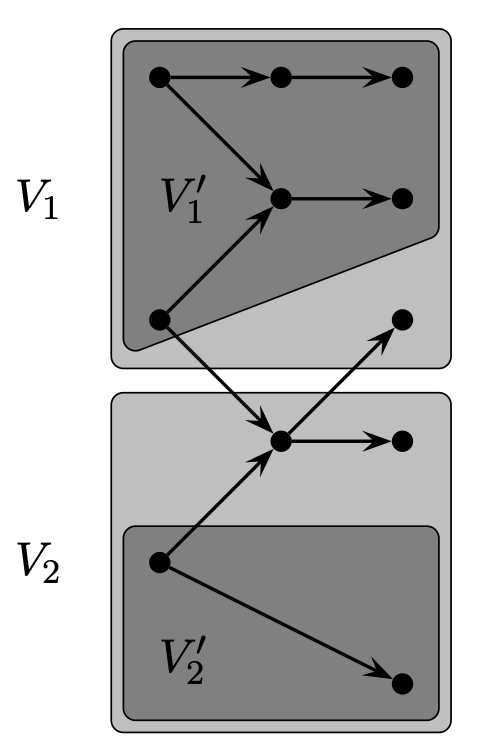
\includegraphics[width=5cm]{chapters/scheduling1/transitive_closure}
% \ifrenderfigures
%   \begin{pspicture}(0,0)(3,4)
%     \pspolygon[linewidth=0.4pt,linearc=0.1,fillstyle=solid,fillcolor=lightgray](-0.4,-0.4)(2.4,-0.4)(2.4,2.4)(-0.4,2.4)% V_1
%     \pspolygon[linewidth=0.4pt,linearc=0.1,fillstyle=solid,fillcolor=gray](-0.3,-0.3)(2.3,-0.3)(2.3,1.3)(-0.3,1.3)% V_1'
%     \pspolygon[linewidth=0.4pt,linearc=0.1,fillstyle=solid,fillcolor=lightgray](-0.4,2.6)(2.4,2.6)(2.4,5.4)(-0.4,5.4)% V_2
%     \pspolygon[linewidth=0.4pt,linearc=0.1,fillstyle=solid,fillcolor=gray](-0.3,2.7)(2.3,3.7)(2.3,5.3)(-0.3,5.3)% V_2'
%     \cnode*(0,1){2.5pt}{a}
%     \cnode*(2,0){2.5pt}{b}
%     \cnode*(1,2){2.5pt}{c}
%     \cnode*(2,2){2.5pt}{d}
%     \cnode*(0,3){2.5pt}{e}
%     \cnode*(2,3){2.5pt}{f}
%     \cnode*(1,4){2.5pt}{g}
%     \cnode*(2,4){2.5pt}{h}
%     \cnode*(0,5){2.5pt}{i}
%     \cnode*(1,5){2.5pt}{j}
%     \cnode*(2,5){2.5pt}{k}
%     \ncline[arrowsize=5pt]{<-}{b}{a}
%     \ncline[arrowsize=5pt]{<-}{d}{c}
%  %   \ncline{->}{d}{a}
%     \ncline[arrowsize=5pt]{<-}{c}{a}
%  %   \ncline{->}{f}{e}
%     \ncline[arrowsize=5pt]{<-}{f}{c}
%     \ncline[arrowsize=5pt]{<-}{g}{e}
%    \ncline[arrowsize=5pt]{<-}{h}{g}
%    \ncline[arrowsize=5pt]{<-}{g}{i}
%  %  \ncline{->}{h}{i}
%    \ncline[arrowsize=5pt]{<-}{k}{j}
%     \ncline[arrowsize=5pt]{<-}{j}{i}
%  %   \ncarc[arcangle=-20]{->}{f}{a}
% %    \ncarc[arcangle=-20]{->}{k}{i}
% %    \ncline{->}{d}{e}
% %   \ncline{->}{h}{e}
%     \ncline[arrowsize=5pt]{<-}{c}{e}
% %        \nput{0}{a}{a}\nput{0}{b}{b}\nput{0}{c}{c}\nput{0}{d}{d}\nput{0}{e}{e}\nput{0}{f}{f}\nput{90}{g}{g}\nput{90}{h}{h}\nput{90}{i}{i}\nput{90}{j}{j}\nput{90}{k}{k}
%         \rput[c](-1,4){$\large{V_1}$}\rput[c](-1,1){$\large{V_2}$}
%     \rput[c](0.2,4){$V_1'$}    \rput[c](0.2,0.2){$V_2'$}
%   \end{pspicture}
%   \fi
  \end{center}
  \caption{Visualization of the partition $V = V_1 \dot{\cup} \ldots \dot{\cup} V_k$ and the induced sets $V_{\ell}' \subseteq V_{\ell}$. Here $\prec$ is the transitive closure of the depicted digraph.}
  \end{figure}
  
We now discuss the analysis. First we show that no cluster is more than a constant factor too large.
%(not quite bounded by $C$, but we can spend another constant factor here). 
\begin{lemma}
One has $|V_{\ell}'| \leq 2c$ for all $\ell=1,\ldots,k$.
\end{lemma}
\begin{proof}
  We know by Theorem~\ref{thm:ProbUSeperatedByClustering} that $\textrm{diam}(V_{\ell}') \leq \textrm{diam}(V_{\ell}) \leq \Delta < \frac{1}{2}$ 
  where the diameter is with respect to $d$.
  Fix a job $j^* \in V_{\ell}'$. 
  Then we know by Lemma~\ref{lem:SmallNeighborhoodOfClosePoints} that there are at most $2c$
  jobs $j$ with $d(j,j^*) \leq \frac{1}{2}$ and the claim follows.
\end{proof}

Next, we see that the clusters respect the precedence constraints.
\begin{lemma}
The solution $V_{1}',\ldots,V_{k}'$ is feasible in the sense that jobs on different machines do not have precedence constraints.
\end{lemma}
\begin{proof}
  Consider jobs processed on different machines, say (after reindexing) $j_1 \in V_{1}'$ and $j_2 \in V_2'$.
   If $j_1 \prec j_2$ then we did \emph{not} have $\Gamma^-(j_2) \subseteq V_2'$. This contradicts
  the definition of the sets $V_{\ell}'$.
\end{proof}


A crucial property that makes the algorithm work is that predecessors of some job $j \in J^*$ must be very close in $d$ distance.
\begin{lemma} \label{lem:DependentJobsInJStarAreCloseInMetricD}
For every $j_1,j_2 \in J^*$ with $j_1 \prec j_2$ one has $d(j_1,j_2) \leq \delta$.
\end{lemma}
\begin{proof}
  We know that
  \[
C^* \stackrel{j_1 \in J^*}{\leq} C_{j_1} \leq C_{j_1} + \underbrace{(1-y_{j_1,j_2})}_{=d(j_1,j_2)} \stackrel{LP}{\leq} C_{j_2} \stackrel{j_2 \in J^*}{\leq} C^* + \delta
  \]
  and so $d(j_1,j_2) \leq \delta$.
\end{proof}

We will use the three statements above together with Theorem~\ref{thm:ProbUSeperatedByClustering} to prove Lemma~\ref{lem:SchedulingOneIntervalViaCKR}.
%\begin{lemma}
%Every job $j^* \in J_0$ is contained in $V_1' \cup \ldots \cup V_k'$ with probability at least $1-8\ln(2n) \cdot \del%ta$.
%\end{lemma}
\begin{proof}[Proof of Lemma~\ref{lem:SchedulingOneIntervalViaCKR}]
  We have already proven that the scheduled blocks have size $|V_{\ell}'| \leq 2c$ and that there are no dependent
  jobs in different sets of $V_1',\ldots,V_k'$. To finish the analysis, 
we need to prove that a fixed job $j^* \in J^*$ is scheduled with good probability.
Consider the set $U := \{ j^* \} \cup (\Gamma^-(j^*) \cap J^*)$ of $j^*$ and its ancestors in $J^*$.

%Since the diameter of $U$ is at most $2\delta$ by Lemma~\ref{lem:DependentJobsInJStarAreCloseInMetricD},  for some fixed $u_1 \in U$  we have that $d(u_1, N(U,2 \Delta)) \leq 2\delta +  2\Delta$.
Since the diameter of $U$ is at most $2\delta$ by Lemma~\ref{lem:DependentJobsInJStarAreCloseInMetricD}, 
%  for every $j_1 \in U$  we have that $d(j^*, j_1) \leq 2\delta +  2\Delta$ by the triangle inequality.
we can use Lemma~\ref{lem:SmallNeighborhoodOfClosePoints}
to see that $ |N(U, \Delta/2)| \leq \frac{c}{1- 2\delta-  \Delta}$.
For our choice of $\Delta = 1/4$ and $\delta \leq \frac{1}{64 \log(4 c) }$, $|N(U,1/8)|\leq 2c$. 
From Theorem~\ref{thm:ProbUSeperatedByClustering},
the cluster is separated with probability at most 
 $\log(4c) \cdot  \frac{8 \delta}{\Delta} \leq \frac{1}{2}$.
\end{proof}

To schedule all jobs in $J^*$, we repeat the clustering procedure $O(\log m)$ times and simply schedule the remaining jobs on one machine. %, then show it is easy to schedule the remaining jobs.
%Recall that we let $m \leq n$ denote the minimum number of machines on which the instance can be scheduled while keeping the optimal makespan.


\begin{lemma} \label{lem: FullSchedulingOneIntervalViaCKR}
  Let $(x,y,C) \in Q(r)$ with $r \geq 5$. Let $C^* \geq 0$ and set $J^* \subseteq \{ j \in J \mid C^* \leq C_j < C^*+\delta\}$.
  Assume that all jobs in $\Gamma^{-}(J^*) \setminus J^*$ have been scheduled respecting precedence constraints.
  Then there is an algorithm with expected polynomial running time that schedules all jobs in $J^*$
  using at most $O(\log m) + \frac{|J^*|}{mc}$ many intervals. 
% Then, we can schedule all jobs in $J^*$ using at most $O(\log m) \cdot c + \frac{|J^*|}{m}$ time slots with probability at least $1-1/n^2$.
\end{lemma}

\begin{proof}
 Our algorithm in Lemma~\ref{lem:SchedulingOneIntervalViaCKR} schedules each $j \in J^*$ in an interval of length $2c$ with probability at least $1/2$.
 We run the algorithm for $2 \log m$ iterations, where input to iteration $k+1$ is the subset of jobs that are not scheduled in the first $k$ iterations. 
 For $k \in \{1,2,\ldots, 2 \log m \}$, let $J^{**}_k$ denote the subset of jobs that are scheduled in the $k^{th}$ iteration, and let $J^*_{k+1} := J^* \setminus \{ \bigcup^{k}_{k' = 1} J^{**}_{k'}$\}.
 In this notation,  $J^*_1 := J^*$.
  % and $J^{**}_0 := \emptyset$.
 Let  $\pazocal{S}(J^{**}_k)$ denote the schedule of jobs $J^{**}_k$  given by Lemma~\ref{lem:SchedulingOneIntervalViaCKR}.
 We schedule $\pazocal{S}(J^{**}_1)$ first, then for $k = 2,\ldots, 2 \log m$, we append the schedule $\pazocal{S}(J^{**}_k)$ after $\pazocal{S}(J^{**}_{k-1})$. %, while inserting $c$ new idle time slots in between.
Let $J' := J^{*}_{2\log m +1}$ denote the set of jobs that were not scheduled in the $2\log m$ iterations.
We schedule all jobs in $J'$ consecutively on a single machine after the completion of $\pazocal{S}(J^{**}_{2 \log m})$.

From our construction, the length of a schedule for  $J^*$, which is a random variable, is at most $O(\log m) +  \lceil \frac{|J'|}{c} \rceil$ many intervals.
For $k \in \{ 1,2, \ldots ,2\log m\}$,  Lemma~\ref{lem:SchedulingOneIntervalViaCKR}  guarantees that each job $j \in J^*_k$ gets scheduled in the $k^{th}$ iteration with probability at least $1/2$.
Therefore, the probability that $j \in J'$,  i.e., it does not get scheduled in the first $2 \log m$ iterations,  is at most $\frac{1}{2m}$.
This implies that $\mathbb{E}[|J'|] \leq \frac{|J^*|} {2m}$.
%We use the standard repetition argument to show that we can schedule all jobs in $J^*$ in at most $O(\log m) \cdot c + \frac{J^*}{m}$ time slots with probability at least $1-1/n^2$.
By Markov's inequality  $\text{Pr}[|J'| > \frac{|J^*|} {m} ] \leq \Pr[|J'| > 2 \cdot \mathbb{E}[|J'|] ] \leq 1/2$.
Hence we can repeat the described procedure until indeed we have a successful run with $|J'| \leq \frac{|J^*|}{m}$ which results in the claimed expected polynomial running time. 
%Consider repeating the above random experiment $2 \cdot \log n$ times.
%The probability that none of these experiments result in $|J'| <  \frac{|J^*|}{m}$ is at most $\frac{1}{n^2}$.
%Therefore, with probability at least $1-1/n^2$, in one of the experiments $|J'| <  \frac{|J^*|}{m}$. 
%Schedule the jobs as in this experiment.

Let us now argue that the schedule of $J^*$ is feasible. 
For $k \in \{ 1,2, \ldots, 2\log m\}$ and any two jobs $j, j' \in \pazocal{S}(J^{**}_k)$,  Lemma~\ref{lem:SchedulingOneIntervalViaCKR}  guarantees that precedence and communication constraints are satisfied.
Furthermore, Lemma~\ref{lem:SchedulingOneIntervalViaCKR} also ensures that there cannot be jobs  $j$, $j'$ such that  $j \in \pazocal{S}(J^{**}_k)$, $j' \in \pazocal{S}(J^{**}_{k'})$ and $j' \prec j$ and $k' > k$. Finally note that every length-$2c$ interval can be split into 2 length-$c$ intervals.
The claim follows.
%Finally, if there are two jobs $j$, $j'$ such that  $j \in \pazocal{S}(J^{**}_k)$, $j' \in \pazocal{S}(J^{**}_{k'})$ and $j \prec j'$  and $k' > k$, then the precedence and communication constraints are satisfied as we insert $c$ idle time slots between $\pazocal{S}(J^{**}_k)$ and $\pazocal{S}(J^{**}_{k'})$
% Thus, it only remains to  argue about the number of time slots used to schedule  $J^*$. 
\end{proof}



\subsection{The Complete Algorithm for $\p \infty \mid \Prec, p_j=1, \Intervals \mid C_{\max}$ }\label{sec:TheCompleteAlgorithm}

Now we have all the pieces to put the rounding algorithm together and prove its correctness.
We partition the jobs into batches, where each batch consists of subset of jobs that have  $C_j$ very close to each other in the LP solution. 
%For $\delta = \frac{1}{16 \log(2C)}$ define $k \in \{0\} \cup \mathbb{N}$, let $J_k = \{j \in J : k \cdot \delta \leq \theta_j \leq (k+1) \cdot \delta\}$.
The complete algorithm is given below.

\begin{center}
 \fbox{
\begin{minipage}{14cm}
  \textsc{The Complete Algorithm} \vspace{1mm} \hrule \vspace{1mm}
  \begin{enumerate*}
  \item[(1)] Solve the LP and let $(x,y,C) \in Q(r)$ with $r \geq 5$.
  \item[(2)] For $\delta = \frac{1}{64 \log(4 c)}$ and $k \in \{0,1,2 \ldots \frac{S-1}{\delta}\}$, define \\
                 $J_k = \{j \in J : k \cdot \delta \leq C_j < (k+1) \cdot \delta\}$ 
  \item[(3)] FOR $k=0$ TO $\frac{S-1}{\delta}$ DO 
      \begin{enumerate*}
        \item[(4)] Schedule the jobs in $J_k$ using the algorithm in Subsection \ref{subsec:singlebatch}.
%        \item Insert $c$ new empty idle slots.
      \end{enumerate*}
 \end{enumerate*}
 \end{minipage}}
\end{center}

Now we finish the analysis of the rounding algorithm.
\begin{proof}[Proof of Theorem~\ref{thm:LPRoundingTheorem}]
  Let us quickly verify that the schedule constructed by our algorithm is feasible.
 For jobs $j_1 \prec j_2$ with $j_1 \in J_{k_1}$ and $j_2 \in J_{k_2}$, the LP implies that $C_{j_1} \leq C_{j_2}$
 and so $k_1 \leq k_2$. If $k_1<k_2$, then $j_1$ will be scheduled in an earlier interval than $j_2$.
 If $k_1=k_2=k$, then 
% For $k = 1,2, \ldots \frac{S-1}{\delta}$  and for any two jobs $j, j' \in J_k$,
 Lemma \ref{lem: FullSchedulingOneIntervalViaCKR}  guarantees that precedence  constraints are satisfied.
%Furthermore, 
%the LP constraints ensures that there cannot be jobs  $j$, $j'$ such that  $j \in J_k$, $j' \in J_{k'}$ and $j' \prec j$ and $k' > k$. 
%Finally, if there are two jobs $j$, $j'$ such that  $j \in J_k$, $j' \in J_{k'}$ and $j \prec j'$  and $k' > k$, then the precedence and communication constraints are satisfied in our schedule as we insert $c$ idle time slots between the schedule of jobs $J_k$ and $J_{k+1}$.

It remains to bound the makespan of our algorithm.  
Lemma \ref{lem: FullSchedulingOneIntervalViaCKR} guarantees that for $k \in \{0,1,2 \ldots \frac{S-1}{\delta}\}$, the jobs in $J_k$ are scheduled using at most $O(\log m) + \frac{|J_k|}{cm}$ many intervals. %time slots with probability at least $1-1/n^2$.
% By applying the union bound argument over all sets $J_k$, with probability at least $1-1/n$ the makespan of our schedule is at most
Then the total number of intervals required by the algorithm is bounded by
$$
\frac{S}{\delta} \cdot O(\log m)  + \sum^{\frac{S-1}{\delta}}_{k = 0} \frac{|J_k|}{cm} =O(\log m \cdot \log c)  \cdot S  +  \frac{|J|}{cm}\leq O(\log m \cdot \log c) \cdot S.
$$
Here we use that $|J| \leq S \cdot cm$ is implied by the constraints defining $K$.
%As both $(S-1) \cdot c$ and  $\frac{J}{m}$ are lowerbounds on the optimal schedule, we complete the proof that the makespan of our algorithm is at most $O(\log m \cdot \log c)$ times the optimal with probability $1-1/n$.
\end{proof}

\begin{remark}
We note that
it is possible to reverse-engineer our solution and write a more compact LP for the problem, enforcing only the necessary constraints such as those given by Lemmas~\ref{lem:metric} and~\ref{lem:clustercapacity}.
%Advantages of such an approach is that S-A hierarchy is needed only in the proof of validity of the LP relaxation, and the final LP has much fewer variables therefore can be solved faster.
We present this compact LP and prove an integrality gap of $\Omega(\sqrt{\log n})$ for it in Section~\ref{sec:IntegralityGap}.
While the compact LP is simpler and could be solved more efficiently,
 we feel that the Sherali-Adams hierarchy gives a more principled and intuitive way to tackle the problem and explain how the LP arises, and hence we choose to present it that way.
\end{remark}

\section{Reductions}\label{sec:Reductions}

We now justify our earlier claim:
the special case $\p \infty \mid \Prec, p_j=1, \Intervals \mid C_{\max}$ indeed captures 
the full computational difficulty of the more general problem $\p \mid \Prec, c \mid C_{\max}$.
The main result for this section will be the following reduction:
\begin{theorem}
	\label{thm:ReductionFromGeneral}
  Suppose there is a polynomial time algorithm that takes a solution for the LP $Q(r)$ with parameters $m,c,S \in \setN$ and $r \geq 5$
  and transforms it into a schedule for $\p \infty \mid \Prec, p_j=1, \Intervals \mid C_{\max}$ using at most $\alpha \cdot S$
  intervals. Then there is a polynomial time  $O(\alpha)$-approximation for $\p \mid \Prec, c \mid C_{\max}$.
%	An $\alpha$-approximation for $\p \infty \mid \Prec, p_j=1, \Intervals \mid C_{\max}$ implies an $O(\alpha)$-approximation for $P \mid \Prec, c \mid C_{\max}$.
\end{theorem}
For the reduction we will make use of the very well known list scheduling algorithm by Graham~\cite{GrahamListScheduling1966}
that can be easily extended to the setting with communication delays.
Here the notation  $\sigma(j) = ([t,t+p_j),i)$ means that the job $j$ is
processed in the time interval $[t,t+p_j)$ on machine $i \in [m]$.
\begin{center}
  \fbox{
\begin{minipage}{14cm}
  \textsc{Graham's List Scheduling} \vspace{1mm} \hrule \vspace{1mm}
  \begin{enumerate*}
  \item[(1)] Set $\sigma(j) := \emptyset$ for all $j \in J$
  \item[(2)] FOR $t=0$ TO $\infty$ DO FOR $i=1$ TO $m$ DO
    \begin{enumerate*}
    \item[(3)] Select any job $j \in J$ with $\sigma(j) = \emptyset$ where every $j' \prec j$ satisfies the following:
      \begin{itemize*}
        \item If $j'$ is scheduled on machine $i$ then $j'$ is finished at time $\leq t$
        \item If $j'$ is schedule on machine $i' \neq i$ then $j'$ finished at time $\leq t-c$
      \end{itemize*}
     \item[(4)] Set $\sigma(j) := ([t,t+p_j),i)$ (if there was such a job)
  \end{enumerate*}
  \end{enumerate*}
 \end{minipage}}
\end{center}
For example, for the problem $\p \mid \Prec \mid C_{\max}$, Graham's algorithm gives a 2-approximation.
The analysis works by proving that there is a chain of jobs covering all time units where not all machines are busy.
Graham's algorithm does \emph{not} give a constant factor approximation for our problem with communication delays,
but it will still be useful for our reduction.



% Our proof will involve considering chains in a fixed schedule. 
%Let $j_{\ell}$ be the job which finishes last in a schedule.
%Consider a \emph{chain} of jobs proceeding each other $j_1 \prec \cdots \prec j_{\ell}$, 
%starting at $j_1$, which has no predecessor, where $j_{i-1}$ is the predecessor of $j_i$ which finishes last.
%Given a schedule for jobs in $J$, we let $\pazocal{Q}(J)$ denote the set of chains.
%For any $Q \in \pazocal{Q}(J)$, the length of chain $Q$ is $|Q|$.
Recall that a set of jobs $\{j_1,\ldots,j_{\ell} \} \subseteq J$ with $j_{\ell} \prec j_{\ell -1} \prec \ldots \prec j_{1}$ is called a \emph{chain}.
We denote  $\pazocal{Q}(J)$ as the set of all chains in $J$ w.r.t. precedence order $\prec$.
\begin{lemma}
	\label{lem:GrahamListScheduling}
  Graham's list scheduling on an instance of $\p \mid \Prec, c \mid C_{\max}$
  results in a schedule with makespan at most
  $\frac{1}{m} \sum_{j\in J}p_j+\max_{Q \in \pazocal{Q}(J)}\{\sum_{j \in Q}p_j+c\cdot (|Q|-1) \}$.
\end{lemma}

  % Let $j_l$ be a job which finishes last and $t_{j_l}$ its starting time.
  % Let $j_{l-1}$ be a predecessor of $j_l$ which finishes last. Then, by our precedence constraint, we have $t_{j_l}\ge t_{j_{l-1}}+p_{j_{l-1}}$. Moreover, if they are scheduled on different machines, then $t_{j_l}\ge t_{j_{l-1}}+p_{j_{l-1}}+C$.
	\begin{figure}
		\begin{center}
            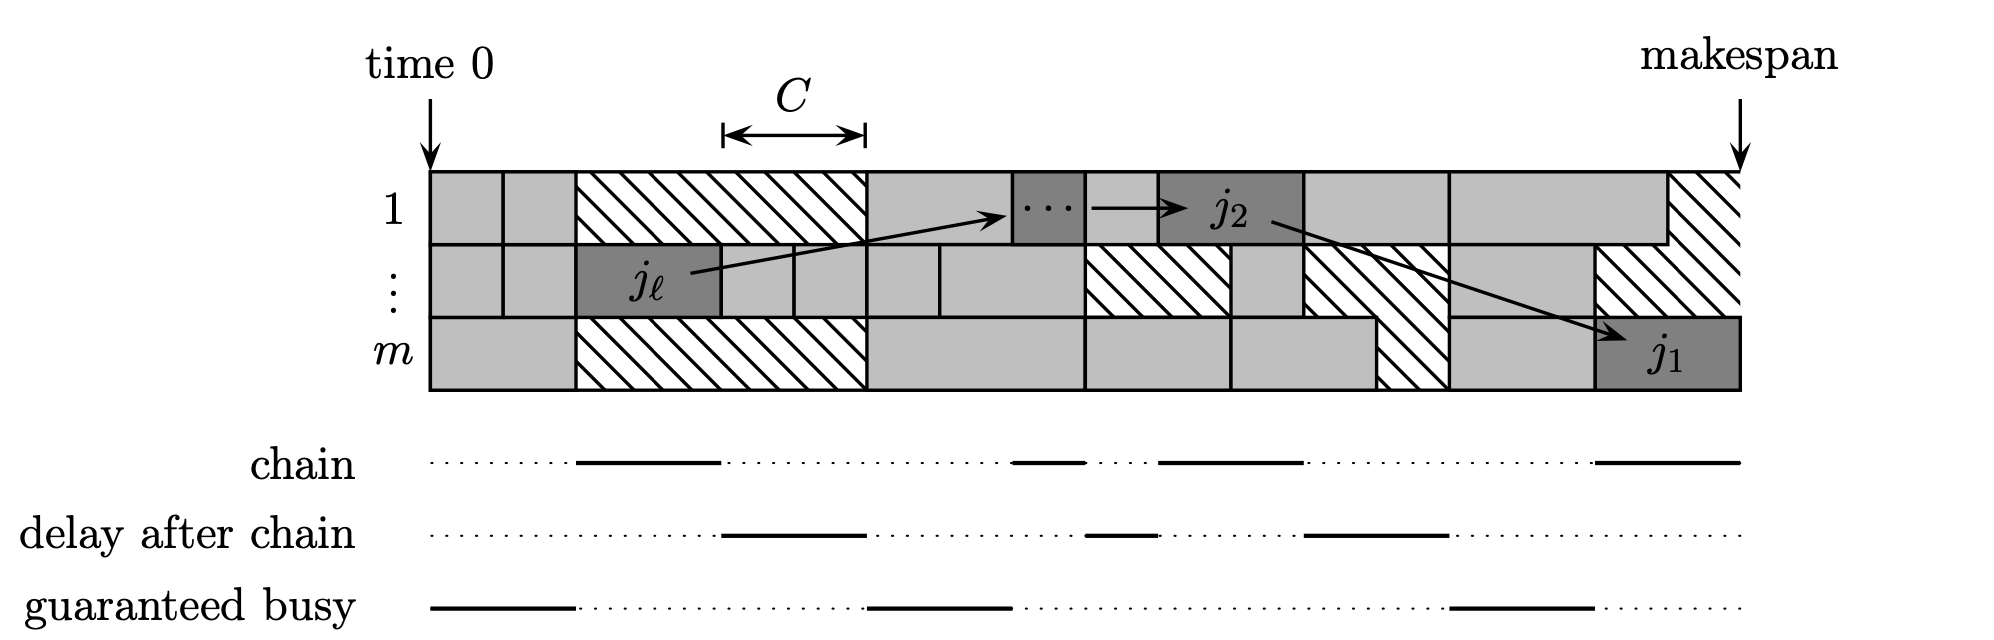
\includegraphics[width=15cm]{chapters/scheduling1/graham_analysis}
% 		\ifrenderfigures
% 			\psset{unit=0.6cm}
% 			\begin{pspicture}(-4,-3)(18,4.5)
% 			\pnode(4,3.5){A}\pnode(6,3.5){B} \ncline[arrowsize=5pt]{|<->|}{A}{B} \naput{$C$}
% 			\psline[fillstyle=vlines](18,0)(0,0)(0,3)(18,3)
% 			\rput[c](0,0){\pspolygon[fillstyle=solid,fillcolor=lightgray](0,0)(2,0)(2,1)(0,1)}
% 			\rput[c](0,1){\pspolygon[fillstyle=solid,fillcolor=lightgray](0,0)(1,0)(1,1)(0,1)}
% 			\rput[c](1,1){\pspolygon[fillstyle=solid,fillcolor=lightgray](0,0)(1,0)(1,1)(0,1)}
% 			\rput[c](0,2){\pspolygon[fillstyle=solid,fillcolor=lightgray](0,0)(1,0)(1,1)(0,1)}
% 			\rput[c](1,2){\pspolygon[fillstyle=solid,fillcolor=lightgray](0,0)(1,0)(1,1)(0,1)}
% 			\rput[c](2,1){\pspolygon[fillstyle=solid,fillcolor=gray](0,0)(2,0)(2,1)(0,1)} \pnode(3,1.5){j1} \rput[c](j1){$j_{\ell}$}
% 			\rput[c](4,1){\pspolygon[fillstyle=solid,fillcolor=lightgray](0,0)(1,0)(1,1)(0,1)}
% 			\rput[c](5,1){\pspolygon[fillstyle=solid,fillcolor=lightgray](0,0)(1,0)(1,1)(0,1)}
% 			\rput[c](6,2){\pspolygon[fillstyle=solid,fillcolor=lightgray](0,0)(2,0)(2,1)(0,1)}
% 			\rput[c](6,1){\pspolygon[fillstyle=solid,fillcolor=lightgray](0,0)(1,0)(1,1)(0,1)}
% 			\rput[c](7,1){\pspolygon[fillstyle=solid,fillcolor=lightgray](0,0)(2,0)(2,1)(0,1)}
% 			\rput[c](6,0){\pspolygon[fillstyle=solid,fillcolor=lightgray](0,0)(3,0)(3,1)(0,1)}
% 			\rput[c](8,2){\pspolygon[fillstyle=solid,fillcolor=gray](0,0)(1,0)(1,1)(0,1)} \pnode(8.5,2.5){j2} \rput[c](j2){$\ldots$}
% 			\rput[c](10,2){\pspolygon[fillstyle=solid,fillcolor=gray](0,0)(2,0)(2,1)(0,1)} \pnode(11,2.5){j3} \rput[c](j3){$j_2$}
% 			\rput[c](9,2){\pspolygon[fillstyle=solid,fillcolor=lightgray](0,0)(1,0)(1,1)(0,1)}
% 			\rput[c](16,0){\pspolygon[fillstyle=solid,fillcolor=gray](0,0)(2,0)(2,1)(0,1)} \pnode(17,0.5){j4} \rput[c](j4){$j_{1}$}
% 			\rput[c](9,0){\pspolygon[fillstyle=solid,fillcolor=lightgray](0,0)(2,0)(2,1)(0,1)}
% 			\rput[c](9,0){\pspolygon[fillstyle=solid,fillcolor=lightgray](0,0)(2,0)(2,1)(0,1)}
% 			\rput[c](11,1){\pspolygon[fillstyle=solid,fillcolor=lightgray](0,0)(1,0)(1,1)(0,1)}
% 			\rput[c](11,0){\pspolygon[fillstyle=solid,fillcolor=lightgray](0,0)(2,0)(2,1)(0,1)}
% 			\rput[c](12,2){\pspolygon[fillstyle=solid,fillcolor=lightgray](0,0)(2,0)(2,1)(0,1)}
% 			\rput[c](14,2){\pspolygon[fillstyle=solid,fillcolor=lightgray](0,0)(3,0)(3,1)(0,1)}
% 			\rput[c](14,1){\pspolygon[fillstyle=solid,fillcolor=lightgray](0,0)(2,0)(2,1)(0,1)}
% 			\rput[c](14,0){\pspolygon[fillstyle=solid,fillcolor=lightgray](0,0)(2,0)(2,1)(0,1)}
% 			\ncline[nodesepA=10pt,nodesepB=10pt,arrowsize=5pt]{->}{j1}{j2}
% 			\ncline[nodesepA=10pt,nodesepB=10pt,arrowsize=5pt]{->}{j2}{j3}
% 			\ncline[nodesepA=10pt,nodesepB=10pt,arrowsize=5pt]{->}{j3}{j4}
% 			\rput[r](-1,-1){chain}
% 			\rput[c](0,-1){\psline[linestyle=dotted,linewidth=0.5pt](0,0)(18,0) \psline[linewidth=1.0pt](2,0)(4,0)\psline[linewidth=1.0pt](8,0)(9,0)\psline[linewidth=1.0pt](10,0)(12,0)\psline[linewidth=1.0pt](16,0)(18,0) }
% 			\rput[r](-1,-2){delay after chain}
% 			\rput[c](0,-2){\psline[linestyle=dotted,linewidth=0.5pt](0,0)(18,0) \psline[linewidth=1.0pt](4,0)(6,0)\psline[linewidth=1.0pt](9,0)(10,0)\psline[linewidth=1.0pt](12,0)(14,0) }
% 			\rput[r](-1,-3){guaranteed busy}
% 			\rput[c](0,-3){\psline[linestyle=dotted,linewidth=0.5pt](0,0)(18,0) \psline[linewidth=1.0pt](0,0)(2,0)\psline[linewidth=1.0pt](6,0)(8,0)\psline[linewidth=1.0pt](14,0)(16,0) }
% 			\rput[c](-0.5,2.5){$1$}  \rput[c](-0.5,1.5){$\vdots$} \rput[c](-0.5,0.5){$m$}
% 			\pnode(0,3){A}\pnode(0,4){B}\ncline[arrowsize=5pt]{->}{B}{A} \nput{90}{B}{time $0$}
% 			\pnode(18,3){A}\pnode(18,4){B}\ncline[arrowsize=5pt]{->}{B}{A} \nput{90}{B}{makespan}
% 			\end{pspicture}
% 			\fi
			\caption{Analysis of Graham's algorithm with communication delay $c$.} 
		\end{center}
  \end{figure}
  \begin{proof} % $
We will show how to construct the chain $Q$ that makes the inequality hold. Let $j_1$ be the job which finishes last
in the schedule produced by Graham's algorithm and let $t_{j_1}$ be its start time. Let $j_2$ be the predecessor of $j_1$
that finishes last. More generally in step $i$, we denote $j_{i+1}$ as the predecessor of $j_i$ that finishes last.
The construction finishes with a job $j_{\ell}$ without predecessors. 
Now let $Q$ be the chain of jobs $j_{\ell} \prec j_{\ell-1} \prec \ldots \prec j_1$. 
The crucial observation is that for any $i \in \{ 1,\ldots,\ell-1\}$, 
either all machines are busy in the time interval $[t_{j_{i+1}}+p_{j_{i+1}}+c,t_{j_{i}})$  or this interval is empty. 
The reason is that Graham's algorithm does not leave unnecessary idle time and would have otherwise processed $j_{i}$ earlier.
It is also true that all $m$ machines are busy in the time interval $[0,t_{j_{\ell}})$.
%    Consider a chain $j_1 \prec \cdots \prec j_{\ell}$ in $\pazocal{Q}(J)$.
%  Let $t_{j_i}$ be the start time of job $j_i$ for $i \in [\ell]$.
%  As Graham's list scheduling leaves no unnecessary idle time on any machine, 
%  if $t_{j_i} \ge t_{j_{i-1}}+p_{j_{i-1}}+C$, then all machines are busy in time interval $[t_{j_{i-1}}+p_{j_{i-1}}+C,t_{j_i})$. 
%  Similarly, all machines are busy in $[0, t_{j_1})$. 
  The total amount of work processed in these busy time intervals is
	\[
	L := m\cdot\Big( t_{j_{\ell}}+ \sum_{i=1}^{\ell-1}\max \{t_{j_{i}}-(c+p_{j_{i+1}}+t_{j_{i+1}}), 0\}\Big)\le \sum_{j \in J} p_j - \sum_{i=1}^{\ell}p_{j_i}.
      \]
      Then any time between $0$ and the makespan falls into at least one of the following categories: 
      (a)~the busy time periods described above, (b)~the times that a job of the chain $Q$ is processed, 
      (c)~the interval of length $c$ following a job in the chain $Q$.
	Thus, we see that the makespan from Graham's list scheduling is at most
	% \[
	% m\cdot[t_{j_1}+ \sum_{i=1}^{l-1} (t_{j_{i+1}}-(C+p_{j_i}+t_{j_i}))]\le \sum_{j \in J} p_j - \sum_{i=1}^{l}p_{j_i},
	% \]
	\[
  t_{j_{1}}+p_{t_{j_{1}}} \leq \frac{L}{m} + \sum_{j \in Q} p_j + c \cdot (|Q|-1) \leq \frac{1}{m} \sum_{j \in J} p_j+\Big(1-\frac{1}{m}\Big)\sum_{j \in Q} p_{j}+c\cdot(|Q|-1).
	\]
	% and the claim follows.	
      \end{proof}

      
 It will also be helpful to note that the case of very small optimum makespan can be well approximated:      
\begin{lemma} \label{lem:PTASForProblemifOPTatMostC}
  Any instance for $\p \mid \Prec, c \mid C_{\max}$ with optimum objective function value at most $c$
  admits a PTAS.
\end{lemma}
\begin{proof}
  Let $J$ be the jobs in the instance and let $\textnormal{OPT}_m \leq c$ be the optimum value.
%  In this case, there is a way to schedule the jobs so that all dependent jobs are scheduled on the same machine.
  Consider the undirected graph $G = (J,E)$ with $\{ j_1,j_2 \} \in E \Leftrightarrow (( j_1 \prec j_2)\textrm{ or }(j_2 \prec j_1))$.
  Let $J = J_1 \dot{\cup} \ldots \dot{\cup} J_N$ be the partition of jobs into connected components w.r.t. graph $G$.
  We abbreviate $p(J') := \sum_{j \in J'} p_j$. The assumption guarantees that the optimum solution cannot afford to pay the communication delay
  and hence there is a length-$c$ schedule that assigns all jobs of the same connected component to the same machine. If we think of a connected component $J_{\ell}$
  as an ``item'' of size $p(J_{\ell})$, then for any fixed $\varepsilon>0$ we can use a PTAS for $\p \mid  \mid C_{\max}$ (i.e. makespan minimization without
  precedence constraints) to find a partition of ``items'' as $[N] = I_1 \dot{\cup} \ldots \dot{\cup} I_m$ with $\sum_{\ell \in I_i} p(J_{\ell}) \leq (1+\varepsilon) \cdot \textnormal{OPT}_m$ in polynomial time~\cite{ApproxAlgoForSchedulingHochbaumShmoysJACM87}. 
  Arranging the jobs $\bigcup_{\ell \in I_i} J_{\ell}$ on machine $i$ in any topological order finishes the argument.
\end{proof}


Additionally, it is a standard argument to convert an instance with arbitrary $p_j$ to an instance where all $p_j \leq n / \varepsilon$,
while only losing a factor of $(1+2\varepsilon)$ in the approximation. 
For $p_{\textrm{max}}:=\max_j p_j$, we simply scale the job lengths and communication delay down by a factor of $\frac{n }{ \varepsilon p_{\textrm{max}}}$
then round them to the nearest larger integer.
This results in at most a $2 \varepsilon$ fraction of the optimal makespan being rounded up and all 
job sizes are integral and at most $n / \varepsilon$. 

Now we can show the main reduction: 
\begin{proof}[Proof of Theorem~\ref{thm:ReductionFromGeneral}] 
	
  Consider an instance of $\p \mid \Prec, c \mid C_{\max}$ with $p_j, c \in \mathbb{N}$.
  Let $J$ denote its job set with precedence constraints, and $\textnormal{OPT}_m(J)$ denote its optimal value where $m$ is the number of
  available machines. 
  By the previous argument, we may assume that $p_j \leq 2n$ for all $j \in J$. 
  Moreover, by Lemma~\ref{lem:PTASForProblemifOPTatMostC} we only need to focus on the case where $\textnormal{OPT}_m(J) > c$.
  We may guess the optimum value of $\textnormal{OPT}_m(J)$ as $\textnormal{OPT}_m(J) \in \{ 1,\ldots,2n^2\}$. 
  %, since otherwise the problem can be solved in polynomial time. 
 % Define $J_S=\{j\in J\mid p_j\le c\}$ as the set of \emph{short} jobs and $J_L=\{j\in J\mid p_j> c\}$
 % as the set of \emph{long} jobs.

  Let $J'$ denote the job set obtained by splitting each job $j \in J$
  into a chain of $p_j$ unit sub-jobs $j^{(1)}\prec \cdots \prec j^{(p_j)}$. 
  Moreover, precedence constraints in $J$ are preserved in $J'$ as we set all 
  predecessors of $j$ to be predecessors of $j^{(1)}$ and all successors of $j$ to be successors of $j^{(p_j)}$, 
  see Figure~\ref{fig:SplittingJobsIntoUnitLengthJobs}.
  \begin{figure}
  \begin{center}
    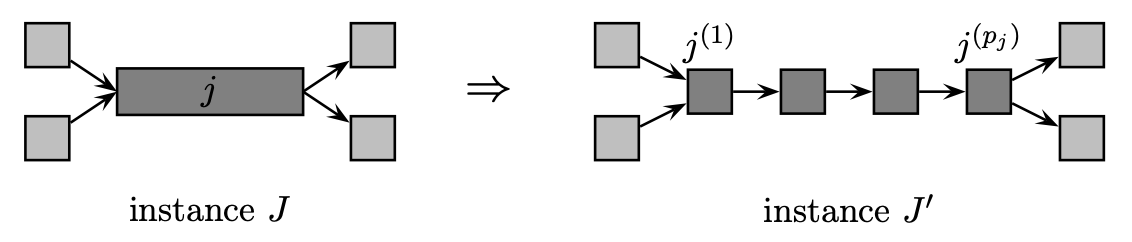
\includegraphics[width=15cm]{chapters/scheduling1/split_jobs}
%   \ifrenderfigures
%     \psset{unit=0.5cm}
%     \begin{pspicture}(0,-2)(8,2)
%     \fnode[framesize=1,fillcolor=lightgray,fillstyle=solid](-1.5,1.5){a}
%     \fnode[framesize=1,fillcolor=lightgray,fillstyle=solid](-1.5,-0.5){b}
%     \fnode[framesize=1,fillcolor=lightgray,fillstyle=solid](5.5,1.5){c}
%     \fnode[framesize=1,fillcolor=lightgray,fillstyle=solid](5.5,-0.5){d}
%     \pspolygon[fillstyle=solid,fillcolor=gray](0,0)(4,0)(4,1)(0,1) \rput[c](2,0.5){$j$}
%     \pnode(0,0.5){jstart}
%     \pnode(4,0.5){jend}
%     \ncline[arrowsize=5pt]{->}{a}{jstart}
%     \ncline[arrowsize=5pt]{->}{b}{jstart}
%    \ncline[arrowsize=5pt]{->}{jend}{c}
%    \ncline[arrowsize=5pt]{->}{jend}{d}
%    \rput[c](8,0.5){\Large $\Rightarrow$}
%    \rput[c](2,-2){instance $J$}
%      \end{pspicture}
%      \begin{pspicture}(-4,-2)(8,2)
%     \fnode[framesize=1,fillcolor=lightgray,fillstyle=solid](-1.5,1.5){a}
%     \fnode[framesize=1,fillcolor=lightgray,fillstyle=solid](-1.5,-0.5){b}
%     \fnode[framesize=1,fillcolor=gray,fillstyle=solid](0.5,0.5){j1} \nput[labelsep=2pt]{90}{j1}{$j^{(1)}$}
%     \fnode[framesize=1,fillcolor=gray,fillstyle=solid](2.5,0.5){j2}
%     \fnode[framesize=1,fillcolor=gray,fillstyle=solid](4.5,0.5){j3}
%     \fnode[framesize=1,fillcolor=gray,fillstyle=solid](6.5,0.5){j4}\nput[labelsep=2pt]{90}{j4}{$j^{(p_j)}$}
%     \fnode[framesize=1,fillcolor=lightgray,fillstyle=solid](8.5,1.5){c}
%     \fnode[framesize=1,fillcolor=lightgray,fillstyle=solid](8.5,-0.5){d}
%     \ncline[arrowsize=5pt]{->}{a}{j1}
%     \ncline[arrowsize=5pt]{->}{b}{j1}
%     \ncline[arrowsize=5pt]{->}{j1}{j2}
%     \ncline[arrowsize=5pt]{->}{j2}{j3}
%     \ncline[arrowsize=5pt]{->}{j3}{j4}
%    \ncline[arrowsize=5pt]{->}{j4}{c}
%    \ncline[arrowsize=5pt]{->}{j4}{d}
%    \rput[c](3.5,-2){instance $J'$}
%  \end{pspicture}
%  \fi
 \caption{Splitting jobs into chains of unit-length jobs.\label{fig:SplittingJobsIntoUnitLengthJobs}}
  \end{center}
  \end{figure}
  We note that $\textnormal{OPT}_m(J') \leq \textnormal{OPT}_m(J)$ as splitting does not increase the value of the optimum.
  Let $\pazocal{S}_m(J')$ be a schedule achieving the value of $\textnormal{OPT}_m(J')$.
  Next, observe that $\pazocal{S}_m(J')$ implies an integral solution for $Q(r)$ with parameters $m,c,S$ where $S := \lceil \textnormal{OPT}_m(J)/c \rceil$ and $r := 5$.
  In particular here we use that if jobs $j_1 \prec j_2$ are scheduled on different machines by $\pazocal{S}_m(J')$, then their starting times differ by at least $c+1$ and hence they are assigned to different length-$c$ intervals.
  
%  Consider the instance of $\p\infty \mid \Prec, p_j=1, \Intervals \mid C_{\max}$ with job set $J'$. 
 % Note that we still count the makespan of a schedule and optimal value is the last time unit of the last time interval.
%  Let $\textnormal{OPT}_{\infty, \text{int}}(J')$ be the optimum value of this instance, where we count the last time unit of the last used interval. %denote its optimal value. 
%  Then $\textnormal{OPT}_{\infty,\text{int}}(J') \le \textnormal{OPT}_{m}(J)+c\le 2\textnormal{OPT}_{m}(J) $. 
  Now we execute the assumed $\alpha$-approximate rounding algorithm and obtain a schedule $\pazocal{S}_{\infty,\text{int}}(J')$
  that uses $T \leq \alpha S$ many intervals. 
%  with makespan 
%  $\textnormal{APX}_{\infty,\text{int}}(J')\le \alpha \cdot \textnormal{OPT}_{\infty,\text{int}}(J')$. 
%  Let $T$ denote the total number of intervals used in $\pazocal{S}_{\infty,\text{int}}(J')$, i.e. $\textnormal{APX}_{\infty,\text{int}}(J')= c\cdot T$. 
  We will use this solution  $\pazocal{S}_{\infty,\text{int}}(J')$ to construct
   a schedule $\pazocal{S}_{\infty}(J)$ for $\p\infty \mid \Prec,c \mid C_{\max}$ 
  with job set $J$ by running split sub-jobs consecutively on the same processor. 
  This will use $4T$ time intervals in total. Recall that $I_s$ denotes the time interval $[sc, (s+1)c)$.
  The rescheduling process is as follows:
	
  For a fixed job $j \in J$, let $I_{s_1}$ be the time interval where $j^{(1)}$ is scheduled in $\pazocal{S}_{\infty,\text{int}}(J')$. 
  Then all other sub-jobs of $j$ should be either scheduled in $I_{s_1}$ or the time intervals after $I_{s_1}$. 
\begin{itemize}	
	\item {\bf Case 1: Some sub-job of $j$ is not scheduled in $I_{s_1}$.}\\
  Schedule job $j$ at the beginning of time interval $I_{4{s_1}+1}$ on a new machine.
  If $j$ is a short job, then it will finish running by the end of the interval. 
  Otherwise $j$ is a long job.
  Let $I_{s_2}$ be the last time interval where a sub-job of $j$ is scheduled in $\pazocal{S}_{\infty,\text{int}}(J')$. 
  Then, the length satisfies $p_j \le c\cdot (s_2-s_1+1)$, 
  which implies that the job finishes by time $c\cdot (4s_1+1)+p_j\le c\cdot(4s_2-1)$.
	
  \item {\bf Case 2: All sub-jobs of $j$ are scheduled in $I_{s_1}$.}\\
  Simply schedule job $j$ during time interval $I_{4s_1}$ on the same machine as in $\pazocal{S}_{\infty,\text{int}}(J')$.  
  % Schedule job $j$ in $S'$ in time interval $I_{4s_1}$ on the same machine as scheduled in $S$. 
  % Note that there could be multiple jobs whose sub-jobs are all scheduled in the same time interval on the same machine, 
  % and in this case their total processing time is upper bounded by $C$.
  % So we can schedule them in arbitrary order on the same machine in one time interval in $S'$.
\end{itemize}	
\begin{figure}
  \begin{center}
    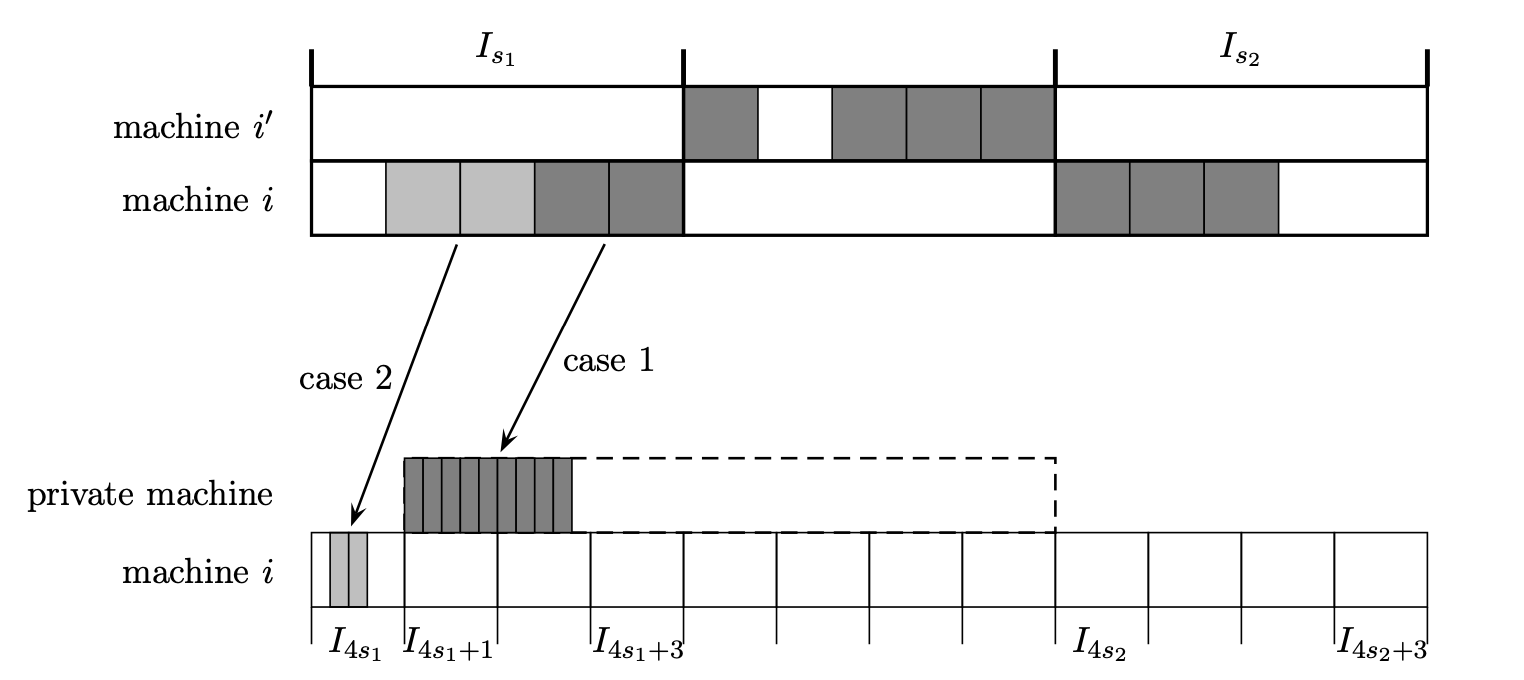
\includegraphics[width=15cm]{chapters/scheduling1/transform}
% \ifrenderfigures
%     \psset{unit=0.8cm}
%     \begin{pspicture}(0,-2)(12,7)
%       % UPPER PART
%      \drawRect{fillstyle=solid,fillcolor=lightgray,linewidth=0.5pt}{1}{4}{1}{1}\drawRect{fillstyle=solid,fillcolor=lightgray,linewidth=0.5pt}{2}{4}{1}{1} \pnode(2,4){caseIIA}
%     \drawRect{fillstyle=solid,fillcolor=gray,linewidth=0.5pt}{3}{4}{1}{1}\drawRect{fillstyle=solid,fillcolor=gray,linewidth=0.5pt}{4}{4}{1}{1}
%     \drawRect{fillstyle=solid,fillcolor=gray,linewidth=0.5pt}{5}{5}{1}{1}\drawRect{fillstyle=solid,fillcolor=gray,linewidth=0.5pt}{7}{5}{1}{1}
%     \drawRect{fillstyle=solid,fillcolor=gray,linewidth=0.5pt}{8}{5}{1}{1}\drawRect{fillstyle=solid,fillcolor=gray,linewidth=0.5pt}{9}{5}{1}{1}
%     \drawRect{fillstyle=solid,fillcolor=gray,linewidth=0.5pt}{10}{4}{1}{1}\drawRect{fillstyle=solid,fillcolor=gray,linewidth=0.5pt}{11}{4}{1}{1}\drawRect{fillstyle=solid,fillcolor=gray,linewidth=0.5pt}{12}{4}{1}{1}
%     \drawRect{linewidth=1.0pt}{0}{5}{5}{1}\drawRect{linewidth=1.0pt}{5}{5}{5}{1}\drawRect{linewidth=1.0pt}{10}{5}{5}{1} \rput[r](-0.5,5.5){machine $i'$}
%     \drawRect{linewidth=1.0pt}{0}{4}{5}{1}\drawRect{linewidth=1.0pt}{5}{4}{5}{1}\drawRect{linewidth=1.0pt}{10}{4}{5}{1}  \rput[r](-0.5,4.5){machine $i$}
%     \rput[c](2.5,6.5){$I_{s_1}$} \rput[c](12.5,6.5){$I_{s_2}$}
%     \multido{\N=0+5}{4}{\psline[linewidth=1.5pt](\N,6)(\N,6.5)}
%     % LOWER PART
%     \drawRect{fillstyle=solid,fillcolor=lightgray,linewidth=0.5pt}{0.25}{-1}{0.25}{1} \pnode(0.5,0){caseIIB}
%     \drawRect{fillstyle=solid,fillcolor=lightgray,linewidth=0.5pt}{0.5}{-1}{0.25}{1}
%     \drawRect{linestyle=dashed}{1.25}{0}{8.75}{1}
%  %   \multido{\N=0.00+1.25}{12}{\drawRect{linewidth=0.5pt}{\N}{0}{1.25}{1}}
%     \multido{\N=0.00+1.25}{12}{\drawRect{linewidth=0.5pt}{\N}{-1}{1.25}{1}}
%     \multido{\N=0.00+1.25}{13}{\psline[linewidth=0.5pt](\N,-1)(\N,-1.5)}
%     \rput[r](-0.5,0.5){private machine}
%     \rput[r](-0.5,-0.5){machine $i$}
%     \rput[c](0.6125,-1.5){$I_{4s_1}$} \rput[c](1.85,-1.5){$I_{4s_1+1}$} \rput[c](4.4,-1.5){$I_{4s_1+3}$}
%     \rput[c](10.6125,-1.5){$I_{4s_2}$} \rput[c](14.4,-1.5){$I_{4s_2+3}$}
%     \ncline[nodesepA=3pt,nodesepB=2pt,arrowsize=5pt]{->}{caseIIA}{caseIIB} \nbput[labelsep=2pt]{case 2}
%     \multido{\N=1.25+0.25}{9}{\drawRect{fillstyle=solid,fillcolor=gray,linewidth=0.5pt}{\N}{0}{0.25}{1}}
%     \pnode(4,4){caseIA}\pnode(2.5,1){caseIB}
%    \ncline[nodesepA=3pt,nodesepB=2pt,arrowsize=5pt]{->}{caseIA}{caseIB} \naput[labelsep=2pt]{case 1}
%     \end{pspicture}   
% \fi
  \caption{Transformation of the schedule $\pazocal{S}_{\infty,\text{int}}(J')$ (top) to $\pazocal{S}_{\infty}(J)$ (bottom), where  $\pazocal{S}_{\infty}(J)$ is compressed by a factor of 4. Here a ``private'' machine for a job $j$ means the machine never processes any job other than $j$.\label{fig:ScheduleTransformationStoSPrime}}
  \end{center}
\end{figure}

% It can be checked that the schedule $S'$ satisfies the precedence constraints and communication delays, which means that it 
 See Figure~\ref{fig:ScheduleTransformationStoSPrime} for a visualization.
 Then  $\pazocal{S}_{\infty}(J)$ is a valid schedule for $\p \infty \mid \Prec,c \mid C_{\max}$, with makespan $\le 4c\cdot T$.
	Moreover, $\pazocal{S}_{\infty}(J)$ satisfies the following:
	\begin{enumerate*}
		\item[(a)]A short job is fully contained in some interval $I_s$.
		
		\item[(b)]A long job's start time is at the beginning of some interval $I_s$.
	\end{enumerate*}
	
  For $\pazocal{S}_{\infty}(J)$, define a new job set $H$. 
  Every long job $j$ becomes an element of $H$ with its original running time $p_j$. 
  Meanwhile, every set of short jobs that are assigned to the same machine in one time interval becomes an element of $H$, 
  with running time equal to the sum of running times of the short jobs merged. 
  To summarize, a new job $h \in H$ corresponds to a set $h \subseteq J$ and $p_h = \sum_{j\in h} p_j$.
	
  We define the partial order $\tilde{\prec}$ on $H$ with $h_1 \tilde{\prec} h_2$ if and only if there are
  $j_1 \in h_1$ and $j_2 \in h_2$ with $j_1 \prec j_2$. 
%  some jobs comprising $j_1$ and $j_2$ in the original job set had precedent constraints. 
One can check that this partial order is well defined. 
  Moreover, by the fact that jobs assigned to the same interval but different machines do not have precedence constraints, 
  the length of the longest chain in $(H,\tilde{\prec})$ in terms of the number of elements is bounded by the number of intervals that are used, 
  which is at most $4T$.
	
  Now run Graham's list scheduling on the new job set $H$ with order $\tilde{\prec}$ and $m$ machines. 
  By Lemma~\ref{lem:GrahamListScheduling}, the makespan of the list scheduling is bounded by  
  $\frac{1}{m} \sum_{h\in H}p_h+\max_{Q \in \pazocal{Q}(H)}\{\sum_{h \in Q}p_h+ c\cdot |Q| \}$.
  As the total sum of the processing times does not change from $J$ to $H$, we see that
  $\frac{1}{m} \sum_{h\in H}p_h \leq \textnormal{OPT}_m(J)$. 
  Moreover, for any chain $Q \in \pazocal{Q}(H)$, $\sum_{h \in Q}p_h$ is no greater than the makespan of $\pazocal{S}_{\infty}(J)$, which is $4cT$.
	Finally, as argued earlier, the chain has $|Q| \leq 4T$ elements.
	Above all, 
  \begin{align*}
    \frac{1}{m} \sum_{h\in H}p_h+\max_{Q \in \pazocal{Q}(H)}\Big\{\sum_{h \in Q}p_h+c\cdot|Q| \Big\} &\le
          \textnormal{OPT}_m(J)+4cT+4cT \\
  &\le \textnormal{OPT}_m(J)+ 8\alpha \cdot cS \\
    &\le \textnormal{OPT}_m(J)+  16\alpha \cdot \textnormal{OPT}_{m}(J) \\
    &=O(\alpha)\cdot \textnormal{OPT}_{m}(J).
	\end{align*}
\end{proof}


%****************************************************************************************************
%%% INTEGRALITY GAP
%****************************************************************************************************
\section{Integrality Gap for the Compact LP}\label{sec:IntegralityGap}

We consider the following layered expander graph from Maiti {et al.}~\cite{MRSSV}. Let $V_1,\ldots,V_L$ be sets of $n$ vertices and for each $j \in V_k$, for $k \in [L-1]$, let $j$ sample $d$ successors from $V_{k+1}$ uniformly at random without replacement. We choose $n = cm/L$ and $c = d^L$, and set $L = \epsilon_1 \sqrt{\log n}$, $d = 2^{\epsilon_2 \sqrt{\log n}}$, and $m=c$. We will fix  $\epsilon_1$ and $\epsilon_2$ as in Maiti et al.; the constants have several specifications, and we will not enumerate all of them, except that $\epsilon_2 \geq 5 \epsilon_1$.
% \footnote{They set parameters in the proof of Proposition 5.4 so that $c^{2+L} < 128 d$, for $c > 32$. Subbing in parameters, $2^{10+5\epsilon_1 \sqrt{\log n}} < c^{2+L} <  2^{7+\epsilon_2 \sqrt{\log n}}$, and so we see that it is necessary for $5\epsilon_1 < \epsilon_2 $.}
 Call this instance $\pazocal{I}$. Note that we have purposefully defined $\pazocal{I}$ so that its partial order is not closed under transitivity, as it will be notationally convenient later to consider the successors and predecessors of a node $j \in V_k$ as the nodes $j'$ in $\Gamma^+(j) \cap V_{k+1}$ and $\Gamma^-(j) \cap V_{k-1}$, respectively.

Our compact LP is the following: 
\begin{align*}
y_{j_1,j_1}&=1 \qquad \forall j_1 \in J\\
y_{j_1,j_2} &= y_{j_2,j_1} \qquad \forall j_1,j_2 \in J\\
1-y_{j_1,j_2} &\leq 1-y_{j_1,j_3} + 1-y_{j_2,j_3} \qquad \forall j_1,j_2,j_3 \in J\\
\sum_{j \in J} y_{j_1,j} &\leq c \qquad \forall j_1 \in J\\
 C_{j_2} &\geq C_{j_1} + (1-y_{j_1,j_2}) \qquad \forall j_1 \prec j_2 \\
  C_j &\geq 0 \quad \forall j \in J \\
  0 \leq y_{j,j'} &\leq 1 \qquad \forall j,j' \in J
\end{align*}


Note the above completely does away with the $x$ variables from LP. 
We will prove the following when parameters for the layered expander graph are specified as above:




\begin{lemma}\label{lem:compactLPbad}
The compact LP has value at most $1$ ($c$-interval) on instance $\pazocal{I}$.
\end{lemma}
Maiti et al. prove that the number of $c$-intervals required for an integral solution to schedule $\pazocal{I}$ is $\Omega(L)$. Combining this with Lemma~\ref{lem:compactLPbad}, we have the following theorem:
\begin{theorem}\label{thm:compactLPintgap}
The compact LP has integrality gap at least $\Omega(\sqrt{\log n})$.
\end{theorem}

Before we begin the proof of Lemma~\ref{lem:compactLPbad} we will define some new terms. First let $\phi(j) : J \rightarrow [L]$ be the map sending each job to its corresponding layer; so $j \in V_{k}$ if and only if $\phi(j) = k$.
Next we let $r(j,j')=\min\{L,s(j,j')\}$, where $s(j,j')$ is the distance between $j$ and $j'$ in the undirected graph, i.e. the number of edges in the shortest path between $j$ and $j'$, when edges of the DAG are made undirected.
Note that for $j \in V_k$ with $j' \in V_{k}\cap \Gamma^+(j)$ and $j'' \in V_{k+2} \cap \Gamma^+(j')$, we have that $r(j,j')=r(j',j'')=1-1/L$ and $r(j,j'') = 1-2/L$. The function $r$ is clearly symmetric. We will show that $r$ satisfies the triangle inequality, since normally it is not the case that a minimum of two metrics is still a metric.

\begin{lemma}\label{lem:triangle_s}
Let $s(j,j')$ be the distance between $j$ and $j'$ in the undirected graph. Then
 $r(j,j') = \min\{L,s(j,j')\}$ satisfies the triangle inequality.
\end{lemma}
\begin{proof}
Fix jobs $j,j',j'' \in J$. Suppose first that $r(j,j') = s(j,j')$. Since $s(j,j') \leq s(j,j'')+s(j'',j')$ and $s(j,j') \leq L$, it follows that $r(j,j') \leq r(j,j'')+r(j'',j')$. 
On the other hand if $r(j,j') =L$, the triangle inequality would only be violated if $j''$ was such that $L > s(j,j'') + s(j'',j')$. However, this inequality implies there is a path from $j$ to $j''$ through $j'$ that has $s(j,j'') + s(j'',j') <L$ edges, which contradicts the definition of $r(j,j')$.
\end{proof}




\begin{proof}[Proof of Lemma~\ref{lem:compactLPbad}]
The set of jobs in instance $\pazocal{I}$ is partitioned into layers $V_1,\ldots,V_L$. For every job $j$, let $j$'s completion time be $C_j = \phi(j)/L$.
For jobs $j,j'$, let $y_{j,j'} = 1-r(j,j')/L$.

Now we check the inequalities of the LP.
We begin by seeing that these $y$ values form a semimetric $d(j,j') = 1-y_{j,j'}$. 
For $j \in J$, $y_{j,j} = 1-0/L=1$ so that $d(j,j)=0$, and $d$ is symmetric since $r(j,j')$ is too. To see that the triangle inequality holds, fix $j,j',j''$ and observe that by Lemma~\ref{lem:triangle_s}.
$$
    1-y_{j,j'} = r(j,j')/L \leq r(j,j'')/L + r(j'',j')/L =  1-y_{j,j''}+ 1-y_{j'',j'}.
$$
Further, we see that for $j,j'$ with $j \prec j'$, $C_j = \phi(j)/L$, $C_{j'} = \phi(j')/L$, and $y_{j,j'} =  1-(\phi(j') - \phi(j))/L$, so that $C_{j'} - C_j \geq 1-y_{j,j'}$. 

The last inequality to check is that for all $j \in J$, $\sum_{j'}y_{j,j'} \leq c$. 
Fix a job $j$, and recall a job $j'$ has $y_{j,j'} = 1-\ell/L$ exactly when $r(j,j')=\ell$. 
Every job, except those in $V_L$, has $d$ successors, and with probability at least $1-n^{-2}$, every job, except those in $V_1$, has at most $d + 10\sqrt{d \log n}$ predecessors. 
Therefore, at most $2^\ell (d+10\sqrt{d \log n})^\ell$ jobs $j'$ have $r(j,j')=\ell$. It follows that 
\begin{align*}
        \sum_{j'} y_{j,j'} &\leq \sum_{\ell =1}^{L-1} 2^{\ell} (d+10\sqrt{d \log n})^{\ell}(1-\ell/L)\\
        &= \frac{2(d+10\sqrt{d \log n})((2(d+10\sqrt{d \log n}))^L-2(d+10\sqrt{d \log n})L+L-1)}{(2(d+10\sqrt{d \log n})-1)^2L} \\
    &\leq \frac{2^{L+1}(d+10\sqrt{d \log n})^{L+1}}{(d+10\sqrt{d \log n})^2}
    \leq 2^{L+1}(d+10\sqrt{d \log n})^{L-1}
    \leq 2^{L+1}(2d)^{L-1}
    \leq d^L=c,
\end{align*}
where the second to last inequality follows from the fact that $d \geq 10 \sqrt{\log n}$, 
and the last inequality follows from the choice of $d$ and $L$ and the fact that $\epsilon_2 \geq 2\epsilon_1$.


% where the last inequality follows 
% since $2^{\epsilon_1 \sqrt{\log n}+1}
%     \leq 2^{\epsilon_2 \sqrt{\log n}}$ 
% from the choice in parameters for $\epsilon_2 \geq 2\epsilon_1$.

% Consider the random experiment of choosing $d$ successors in $V_{k+1}$ for every job $j \in V_k$. Jobs $j' \in V_{k+1}$ may have more than $d$ predecessors, therefore increasing the number of jobs $j''$ with $r(j,j'')<L$. 
% We can perform the same calculation to upper bound $\sum_{j'}y_{j,j'}$ as before, this time exchanging $d$ for $d+10\sqrt{d \log n}$:

\end{proof}




%****************************************************************************************************
%%% COMPLETION TIME RESULT
%****************************************************************************************************


\section{Minimizing Weighted Sum of Completion Times}

To illustrate the generality of our framework we show that it can be extended to handle different objective
functions, in particular we can minimize the \emph{weighted sum of completion times} of the jobs. Here we
restrict to the simplest case where jobs have unit length and an unbounded number of machines are available. 
In the 3-field notation, this problem is denoted by $\p \infty \mid \Prec, p_j=1, c \mid \sum_{j}w_j C_j$.
The input for this problem is the same as for the makespan minimization problem except that each job $j$ now has a weight $w_j \geq 0$. 

%Without loss of generality, we assume that weights are positive integers.
The goal is to minimize the objective function $\sum_{j} w_j C_j$, where $C_j$ is the completion time of $j$, which is defined as the time slot in which job $j$ is scheduled. 
%Since our main aim is  to illustrate the generality of our framework, we only consider case when jobs have unit length and the number of machines is unbounded. 

Note that the LP $Q(r)$ has variables $C_j$ that denote the index of the length-$c$ interval where $j$ is being scheduled.
A natural approach would be to interpret $c \cdot C_j$ as the completion time of job $j$ and minimize $\sum_{j \in J} w_j \cdot c \cdot C_j$ over $Q(r)$. Then the rounding algorithm from Section~\ref{sec:approximation_for_pinfty}
will indeed schedule each job $j$ so that the completion time is at most $(O(\log c \cdot \log n) \cdot C_j+ \Theta(\log n)) \cdot c$.
We can observe that if a $O(\log c \cdot \log n)$ approximation is the goal, then this argument suffices for all jobs $j$
where the LP solution has $C_j \geq \Omega(\frac{1}{\log c})$ --- but it fails for jobs with $0 \leq C_j \ll 1$.

%Our algorithm for the completion time problem follows a similar framework as the makespan problem.
%In fact, it is easy to see that for all the jobs for which the makespan LP pays a cost of $\Theta(c)$ (that is, $C_j$ variables in the LP is at least $\Theta(1)$), the makespan algorithm already achieves $O(\log n \cdot \log c)$ approximation for the completion times of jobs.
%We only need to argue for those jobs whose completion time in the LP solution is significantly smaller than $c$. 

\subsection{The linear program}
In order to address this case, we first start with a more general  LP relaxation compared to the makespan result
which tracks the actual time slot where the jobs are processed, rather than just the interval.
Again, we use the parameter $m \in \setN$ to denote the number of machines that we allow the LP to use (one can set $m := n$)
and the parameter $S \in \setN$ to denote the number of intervals that we allow for the time horizon. We abbreviate $T := S \cdot c$ as the number of
time slots. Note that $T \leq nc$ always suffices for any non-idling schedule. We index time slots as $[T] := \{ 1,\ldots,T\}$
and consider an interval as a discrete set of slots $I_s := \{ cs+1,\ldots,c(s+1)\}$ where $s \in \{ 0,\ldots,S-1\}$.

Recall that in the makespan result $x_{j,i,s}$ variables indicated if job $j$ got scheduled on machine $i$ in the interval $s$. %\rem{T: In Sec 1-4 we use $x_{j,i,s}$ so I am switching to that order here as well.}
Here, we introduce additional variables of the form $z_{j,i,t}$ which indicate if job $j$ is scheduled on machine $i$ at time $t \in [T]$.
% (Note that completion time of any non-idling schedule is at most $nc$).
The variables $x_{j,i,s}$ are fully determined by summing over appropriate variables $z_{j,i,t}$, but we retain
them for  notational convenience.
Further, similar to our makespan result, we  impose an interval structure on the optimal solution and lose an $O(1)$ factor in the approximation ratio.
%Recall that $S$ denotes the number of intervals used in an optimal solution.



Let $\tilde{K}$ be the set of fractional solutions to the following LP.
\begin{eqnarray*}
  \sum_{i \in [m]} \sum_{t \in [T]} z_{j,i,t} &=& 1 \quad \forall j \in J \\
  \sum_{j \in J} z_{j,i,t} &\leq& 1 \quad \forall i \in [m] \;\; \forall t \in [T] \\
  \sum_{t' < t} \sum_{i \in [m]} z_{j_1,i,t'} &\geq& \sum_{t' \leq t} \sum_{i \in [m]} z_{j_2,i,t'} \quad \forall j_1 \prec j_2 \;\;\forall t \in [T] \\
   \sum_{t \in I_s} z_{j,i,t} &=& x_{j,i,s} \quad \forall j \in J \;\; \forall s \in \{ 0,\ldots,S-1\} \\
  0 \leq z_{j,i,t} &\leq& 1 \quad \forall j \in J, i \in [m], t \in [T] \\
\end{eqnarray*}

Similar to the makespan LP, let $\tilde{Q}(r)$ be the set of feasible solutions  $(x,y, z,C)$ to the following LP:
\begin{eqnarray*}
\text{Minimize}  &&\sum_{j \in J} w_j \cdot C_j \\
  y_{j_1,j_2} &=& \sum_{s \in \{ 0,\ldots,S-1\}} \sum_{i \in [m]} x_{(j_1,i,s),(j_2,i,s)} \\
  C_{j_2} &\geq& C_{j_1} + (1-y_{j_1,j_2}) \cdot c \quad \forall j_1 \prec j_2 \\
  C_j &=& \sum_{i \in [m]} \sum_{t \in [T]} z_{j,i,t} \cdot t \quad \forall j \in J \\
  (x,z) &\in& SA_r(\tilde{K})
\end{eqnarray*}


%As before, we require that $r \geq 5$. 
Note that the $C_j$ variables in this LP relaxation denote the actual completion time of $j$ unlike their role in the makespan result, where they were used to indicate the interval in which $j$ was scheduled.
% We also add the constraint that $C_j \geq \sum_{i} \sum_{t} z_{ijt} \cdot t$, although they may already be implied by our relaxation.
The main technical result for this section is the following:
\begin{theorem} \label{thm:WeightedSumOfComplTimeMainTechResult}
Consider an instance for $\p \infty \mid \Prec, p_j=1, c \mid \sum_{j}w_j C_j$ and 
a solution $(x,y,z,C) \in \tilde{Q}(r)$ with $r \geq 5$. % with parameters $m,c,S,T \in \setN$.
Then there is a randomized algorithm with expected polynomial running time that finds a feasible schedule so that
(i) $\E[C_j^A] \leq O(\log c \cdot \log n) \cdot C_j$ and (ii) $C_j^A \leq O(\log c \cdot \log n) \cdot C_j + O(\log n) \cdot c$ for all $j \in J$, where $C_j^A$ is the completion time of job $j$.
\end{theorem}
We briefly describe how Theorem~\ref{thm:WeightedSumOfComplTimeMainTechResult} implies the approximation algorithm
promised in Theorem~\ref{thm:maincomp_sched1}:
\begin{proof}[Proof of Theorem~\ref{thm:maincomp_sched1}]
Note that strictly speaking $\tilde{Q}(r)$ is not actually a relaxation of  $\p \infty \mid \Prec, p_j=1, c \mid \sum_{j}w_j C_j$. However one can take an optimum integral schedule and insert $c$ idle time slots every $c$ time units and obtain a feasible solution for $\tilde{Q}(r)$. This increases the completion time of any job by at most a factor of 2.
Then we set $r := 5$ and $m := n$ and solve the LP $\tilde{Q}(r)$ in time polynomial in $n$.
Now consider the randomized schedule from Theorem~\ref{thm:WeightedSumOfComplTimeMainTechResult} with completion times $C_j^A$. Then the expected objective function is
 $\E[\sum_{j \in J} w_j \cdot C^A_j] \leq O(\log n \cdot \log c) \cdot \big( \sum_{j \in J} w_j \cdot C_j \big)$.
 Markov's inequality guarantees that we can find in expected polynomial time a schedule that satisfies this inequality if we increase the right hand side by a constant factor. This completes the proof.
 %satisfies  $ \sum_{j} w_j \cdot C^A_j \leq O(\log n \cdot \log c) \cdot \left( \sum_{j} w_j \cdot C_j \right)$, which completes the proof.
\end{proof}




\subsection{The Rounding Algorithm}
Let $(x, y, z, C)$ be an optimal solution to the LP relaxation $\tilde{Q}(r)$ with $r \geq 5$.
It remains to show Theorem~\ref{thm:WeightedSumOfComplTimeMainTechResult}.
We partition the jobs based on their fractional completion times. 
For  $\delta = \frac{c}{64 \log(4c)}$
and  $k \geq 0$, let $J_k := \{j \in J : k \cdot \delta \leq C_j < k \cdot \delta\}$. 

%$$J_0 := \left \{j \in J:  C_j \leq c \right\}$$
%as the set of jobs with the fractional completion time in the LP solution not greater than $c$.
 
We give a separate  algorithm for scheduling jobs in $J_0$ within an interval of length at most $O(\log n) \cdot c$.
Now consider the remaining jobs.
For $k = 1,2,...$, we schedule jobs in the set $J_k$  using the algorithm from Section~\ref{sec:TheCompleteAlgorithm},


inserting $c$ empty time slots between the schedule of jobs in the set $J_k$ and $J_{k+1}$.
Let $C^{A}_j$ denote the completion time of job $j$ in our algorithm.

\begin{lemma}
\label{lem:comp5}
For $k \geq 1$, consider a job $j \in J_k$. Then deterministically $C^{A}_j \leq O(\log n \cdot \log c) \cdot C_j $.
\end{lemma}

\begin{proof}
The claim follows from repeating the arguments in Lemma \ref{lem: FullSchedulingOneIntervalViaCKR}, so we only give a sketch here. 
Fix $k$ and consider scheduling the jobs in the set $J_k$ using the procedure described in Lemma \ref{lem: FullSchedulingOneIntervalViaCKR}, where we repeat the CKR clustering algorithm for $k = \{1,2, \ldots 2\log n\}$ iterations. 
Then the expected number of jobs that did not get scheduled in the first $2\log n$ iterations is at most $\frac{|J_k|}{n^2} < 1$. Therefore, in expected polynomial time we can find a schedule such that  $C^{A}_j  \in [2\log n \cdot O(c) \cdot k, 2\log n \cdot O(c) \cdot (k+1)]$.
From the definition of set $J_k$,  the fractional completion time $C_j$ of every job $j$ in $J_k$ is at least $k \cdot \frac{c}{64 \log (4c)}$ in the LP solution.
This completes the proof.
\end{proof}

The only new ingredient  for the completion time result is scheduling the jobs in the set $J_0$. 
For $j \in J_0$, let $t^*_j$ denote the earliest time instant $t$ at which the job is  scheduled to a fraction of at least $1-\varepsilon$ in the LP solution. Here $0<\varepsilon<1$ is a small constant that we determine later.
In scheduling theory this time is also called \emph{$\alpha$-point} with $\alpha = 1-\varepsilon$.
Formally 
\begin{equation} \label{eq:AlphaPoints}
  t^*_j := \min \left\{t' \in [T]:  \sum_{i=1}^m  \sum^{t'}_{t = 1} z_{j,i,t} \geq 1-\varepsilon   \right\}
\end{equation}


We use the same semimetric $d(j_1,j_2) := 1-y_{j_1,j_2}$ as in Section~\ref{sec:approximation_for_pinfty} and schedule jobs in $J_0$ using the following procedure.

\begin{center}
  \fbox{
\begin{minipage}{14cm}
  \textsc{Schedule For $J_0$} \vspace{1mm} \hrule \vspace{1mm}
\begin{enumerate*}
  \item[(1)] Run a CKR clustering on the semimetric space $(J_0,d)$ with parameter $\Delta := \frac{1}{12}$ and let $V_1,\ldots,V_k$ be the clusters.
  \item[(2)] Let $V_{\ell}' := \{ j \in V_{\ell} \mid (\Gamma^-(j) \cap J_0) \subseteq V_{\ell}\}$ for $\ell = 1,\ldots,k$.
  \item[(3)] For all $\ell=1,\ldots,k$ assign jobs in $V_{\ell}'$ on  a single machine and schedule them in the increasing of order of $t^*_j$ values breaking ties in an arbitrary manner.
  \item[(4)] Insert a gap of $c$ time slots.
  \item[(5)] Let $J'_0 \subseteq J_0$ be the set of jobs that did not get scheduled in steps (1) - (3). Use Lemma \ref{lem: FullSchedulingOneIntervalViaCKR} to schedule $J'_0$.
  \end{enumerate*}
\end{minipage}}
\end{center}


\begin{lemma}\label{l:ctsecondbatch1}
  For a job $j_1 \in J_0$, the probability that $j_1$ gets scheduled in step (5) of the algorithm, 
i.e., $j_1 \in J'_0$, is at most  $O(\log c) \cdot \frac{C_{j_1}}{c}$.
\end{lemma}
\begin{proof}
  The arguments are a slight refinement of Lemma~\ref{lem:SchedulingOneIntervalViaCKR}.
  Consider the set $U := \{ j_1 \} \cup (\Gamma^{-}(j_1) \cap J_0)$ of $j_1$ and its ancestors. If $j_0 \prec j_1$, then $0 \leq C_{j_0} + c \cdot d(j_0,j_1) \leq C_{j_1}$ by the LP constraints and so $d(j_0,j_1) \leq \frac{C_{j_1}}{c}$.
  Then the diameter of $U$ with respect to semimetric $d$ is bounded by $2C_{j_1}$ and hence by Theorem~\ref{thm:ProbUSeperatedByClustering}.(b) the probability that $U$ is separated is bounded by $\ln(2|N(U,\Delta/2)|) \cdot \frac{4 \textrm{diam}(U)}{\Delta} \leq O(\log c) \cdot \frac{C_{j_1}}{c}$.
\end{proof}




The next lemma follows from repeating the arguments in Lemma \ref{lem:comp5}. 
\begin{lemma}
\label{l:ctsecondbatch2}
For a job $j \in J_0$, condition on the event that $j \in J'_0$.  Then, $C^A_j|_{(j \in J'_0)} \leq O(\log n ) \cdot c$.
\end{lemma}

%We assume that $(x,y,z,C)$ is a solution to $Q(r)$ with $r \geq 5$ and
We can now prove that every cluster $V_{\ell}'$ can be scheduled on one machine so that the completion time
of any job is at most twice the LP completion time.
%As before, $d$ is the semimetric defined by $d(j_1,j_2) := 1-y_{j_1,j_2}$. $
\begin{lemma} \label{l:ctsecondbatch}
  For a small enough constant $\varepsilon > 0$ ($\varepsilon = \frac{1}{12}$ suffices) the following holds: 
  Let $U \subseteq J$ be a set of jobs 
  with $\textrm{diam}(U) \leq \varepsilon$ w.r.t. distance $d$. Define $t_j^*$ as in Eq~\eqref{eq:AlphaPoints} and
%  \[
%    t^*_j := \min\Big\{ t' \in [T] \mid \sum_{i=1}^m \sum_{t=1}^{t'} z_{j,i,t} \geq 1-\varepsilon \Big\} 
%  \]
  schedule the jobs in $U$ in increasing order of $t_j^*$ on one machine and denote the completion time of $j$ by $C_j^A$.
  Then, in expectation $C_j^A \leq 2 t_j^*$ for every $j \in U$.
\end{lemma}


\begin{proof}
  Let us index the jobs in $U = \{ j_1,\ldots,j_{|U|}\}$ so that $t_{j_1}^* \leq \ldots \leq t_{j_{|U|}}^*$.
  Suppose for the sake of contradiction that there is some job $j_N$ with $C_{j_N}^A > 2 t_{j_N}^*$.
  Abbreviate $U^* := \{ j_1,\ldots,j_N\}$ and $\theta^* := t_{j_N}^*$ so that  $1 \leq t_j^* \leq \theta^*$ for $j \in U^*$.
  We observe that $|U^*| = \sum_{j \in U^*} p_j > 2\theta^*$. Then we have
  \[
(A) \;\; \sum_{j \in U^*} \sum_{i \in [m]} \sum_{t=1}^{\theta^*} z_{j,i,t} \geq (1-\varepsilon)|U^*|, \quad (B) \;\; \sum_{j \in U^*} y_{j,j_N} \geq (1-\varepsilon)|U^*|, \quad  (C) \;\; \sum_{i \in [m]} \sum_{t=1}^{\theta^*} z_{j_N,i,t} \geq 1-\varepsilon
\]
where $(A)$ and $(C)$ are by definition of $t_j^*$ and $(B)$ follows from $\textrm{diam}(U^*) \leq \textrm{diam}(U) \leq \varepsilon$.
Intuitively, this means that we have $|U^*| > 2\theta^*$ many jobs that the LP schedules almost fully
on slots $\{1,\ldots,\theta^*\}$ while (B) means that the jobs are almost fully scheduled on the same machine.

As before, we will use the properties of the Sherali-Adams hierarchy to formally derive a contradiction.
We know by Lemma~\ref{lem:PropertiesOfSAforSchedulingWithCommDelaysLP}\footnote{Strictly speaking, Lemma~\ref{lem:PropertiesOfSAforSchedulingWithCommDelaysLP} describes the SA properties for LP $Q(r)$, but an absolutely analogous statement holds for $\tilde{Q}(r)$.} that there is a distribution  $(\tilde{x},\tilde{z},\tilde{y}) \sim \pazocal{D}(j_N)$ so that $\E[\tilde{x}_{j,i,s}] = x_{j,i,s}$, $\E[\tilde{z}_{j,i,t}]=z_{j,i,t}$ and $\E[\tilde{y}_{j_1,j_2}]=y_{j_1,j_2}$ while the variables involving job $j_N$ are integral, i.e.

$\tilde{x}_{j_N,i,s},\tilde{z}_{j_N,i,t} \in \{ 0,1\}$.
Consider the three events
  \[
(A') \sum_{j \in U^*} \sum_{i \in [m]} \sum_{t=1}^{\theta^*} \tilde{z}_{j,i,t} \geq (1-3\varepsilon)|U^*|, \quad (B')  \sum_{j \in U^*} \tilde{y}_{j,j_N} \geq (1-3\varepsilon)|U^*|, \quad   (C') \sum_{i \in [m]} \sum_{t=1}^{\theta^*} \tilde{z}_{j_N,i,t} = 1.
\]
Then by Markov inequality $\Pr[A'] \geq \frac{2}{3}$, $\Pr[B'] \geq \frac{2}{3}$ and $\Pr[C'] \geq 1-\varepsilon$, and so by the union bound
$\Pr[A' \wedge B' \wedge C'] > 0$, assuming $\varepsilon < \frac{1}{3}$.
Fix an outcome for $(\tilde{x},\tilde{y},\tilde{z})$ where the events $A',B',C'$ happen and let $i_N \in [m],t_N \in \{ 1,\ldots,\theta^*\}$ be the indices with $\tilde{z}_{j_N,i_N,t_N}=1$. Then the interval index with $t_N \in I_{s_N}$ satisfies $\tilde{x}_{j_N,i_N,s_N}=1$. Hence
\begin{eqnarray*}
  (1-3\varepsilon) |U^*| &\stackrel{(B')}{\leq}& \sum_{j \in U^*} \tilde{y}_{j,j_N} \stackrel{LP}{=} \sum_{j \in U^*} \sum_{i \in [m]} \sum_{s \in \{ 0,\ldots,S-1\}} \tilde{x}_{(j,i,s),(j_N,i,s)} \stackrel{\tilde{x}_{j_N,i_N,s_N}=1}{=} \sum_{j \in U^*} \tilde{x}_{j,i_N,s_N} \\
  &\stackrel{LP}{\leq}& \underbrace{\sum_{j \in U^*} \sum_{t=1}^{\theta^*} \tilde{z}_{j,i_N,t}}_{\leq \theta^*\textrm{ by LP}} + \underbrace{\sum_{j \in U^*} \sum_{t > \theta^*} \tilde{z}_{j,i_N,t}}_{\leq 3\varepsilon |U^*|\textrm{ by }(A')} \leq \theta^* + 3\varepsilon |U^*|
\end{eqnarray*}
Rearranging gives $|U^*| \leq \frac{1}{1-6\varepsilon} \theta^*$, which is a contradiction for $\varepsilon \leq \frac{1}{12}$.
\end{proof}



\begin{lemma}
\label{l:jnot}
For a job $j \in J_0$, condition on the event that it got scheduled in the step (3) of the algorithm. 
Then, $C^A_j |_{(j \not \in J'_0)} \leq O(C_{j})$.
\end{lemma}
\begin{proof}
  Consider a job $j \in J_0 \setminus J_0'$. Then $j \in V_{\ell}'$ and by construction, the
  set $V_{\ell}'$ has diameter at most $\Delta = \frac{1}{12}$ w.r.t. $d$.
  Then Lemma~\ref{l:ctsecondbatch} guarantees that the completion time is $C_j^A \leq 2t_j^*$ where
  we set $\varepsilon = \frac{1}{12}$.
  Finally note that an $\varepsilon$-fraction of $j$ was finished at time $t_j^*$ or later and hence
  $C_j = \sum_{i \in [m]} \sum_{t \in [T]} z_{j,i,t} \cdot t \geq \varepsilon \cdot t_j^*$. 
 Putting everything together we obtain $C_j^A \leq \frac{2}{\varepsilon} C_j$.
\end{proof}



We have everything to finish the proof of the completion time result.

\begin{proof}[ Proof of Theorem \ref{thm:WeightedSumOfComplTimeMainTechResult}]
From Lemma \ref{lem:comp5}, for $k \geq 1$ and  $ j \in J_k$,  we have deterministically $C^{A}_j \leq O(\log n \cdot \log c) \cdot C_j$.
Now consider a job $j \in J_0$. Then,
\begin{eqnarray*}
\E[C^A_j]  &=& \E[C^A_j | (j \not \in J'_0)] \cdot \text{Pr}[ (j \not \in J'_0)] + \E[C^A_j | (j  \in J'_0)] \cdot \text{Pr}[ (j \in J'_0)]  \\
&\leq& O(C_j) + O(\log c) \cdot \frac{C_j}{c}  \cdot O(\log n) \cdot c \quad (\text{from Lemmas } \ref{l:ctsecondbatch1}, \ref{l:ctsecondbatch2}, \ref{l:jnot} ) \\
&\leq& O(\log n \cdot \log c) \cdot O(C_j)
\end{eqnarray*}
Finally note that the completion time of a job $j \in J_0$ is always bounded by $C_j^A \leq O(\log n) \cdot c$. The claim follows.
%where in the last inequality we used that $\kappa_j\leq \frac{1}{12}$ and that the LP constraints guarantee $C_j \geq \kappa_j \cdot c$. 
%Therefore, $ \sum_{j} w_j \cdot \E[C^A_j] \leq O(\log n \cdot \log c) \cdot \left( \sum_{j} w_j \cdot C_j \right)$.
%Markov's inequality guarantees that we can find in expected polynomial time a schedule that satisfies  $ \sum_{j} w_j \cdot C^A_j \leq O(\log n \cdot \log c) \cdot \left( \sum_{j} w_j \cdot C_j \right)$, which completes the proof.
\end{proof}


\section*{Conclusion}
We gave a new framework for scheduling jobs with precedence constraints and communication delays based on metric space clustering.
Our results take the first step towards resolving several important problems in this area. 

One immediate open question is to understand whether our approach can yield a constant-factor approximation for $\p \mid \Prec, c \mid \Cmax$.
A more challenging problem is to handle {\em non-uniform} communication delays in 
the problem $\p \mid \Prec, c_{jk} \mid \Cmax$, where $c_{jk}$ is the communication delay between jobs $j \prec k$.







\newpage

\chapter{Scheduling with Communication Delays on Related Machines}\label{chapter: S2}

  \section{Introduction}
  We consider the problem of scheduling jobs with precedence and communication delay constraints on {\em related machines.}
  This classic model  was first introduced by Rayward-Smith~\cite{RAYWARDSMITH1987} and Papadimitriou and Yannakakis~\cite{PapadimitriouY90}.
  In this problem we are given a set  $J$ of $n$ jobs, where each job $j$ has a processing length $p_j  \in \setZ_+$ and a weight $w_j \in \setZ_+$.
  The jobs need to be scheduled on $m$ related machines, where machine $i \in [m]$ has speed $s_i  \in \setZ_+$.
  If a job $j$ with processing length $p_j$ is scheduled on the machine $i$, then it requires  $p_j/s_i$ time units to complete.
  In addition, we are  given a {\em communication delay parameter} $c \in  \setZ_{\ge 0}$.
  The jobs have precedence and communication delay constraints, which are given by a partial order $\prec$. 
  A constraint $j \prec j'$ encodes that job $j'$ can only start after job $j$ is completed.
  Moreover, if $j \prec j'$ and $j$, $j'$ are scheduled on {different machines}, then $j'$ can only start executing at least $c$ time units after $j$ had finished. 
  On the other hand,  if $j$ and $j'$ are scheduled on the {same machine}, then $j'$ can start executing immediately after $j$ finishes. 
  The goal is to schedule jobs {\em non-preemptively} so as to minimize a certain objective function.
  In a non-preemptive schedule, each job $j$ needs to be  assigned to a single machine $i$ and executed during a contiguous time interval of length $p_j/s_i$.
  
  \medskip
  We focus on two widely studied objective functions: (1) minimizing the weighted sum of completion times of jobs, and (2) minimizing the makespan.
  In the standard 3-field notation\footnote{
  We adopt the convention of \cite{GLLR79,VeltmanLL90}, where the respective fields denote:
      \textbf{(1) machine environment:} $Q$ for related machines, $P$ for identical machines,
      \textbf{(2) job properties:} $\Prec$ for precedence constraints; $c$ for communication delays of length $c$; $p_j = 1$ for unit length case,
      \textbf{(3) objective:} $\Cmax$ for minimizing makespan, $\wjcj$ for minimizing weighted sum of completion times.
  },
  these problems are denoted by $Q \mid \Prec, c \mid \wjcj$ and $Q  \mid \Prec, c \mid \Cmax$, respectively.
  In the presence of precedence and communication delay constraints, the weighted completion time objective is more general than the makespan, in the sense that one can use an approximation algorithm for the completion time objective to obtain a comparable result for the makespan.
  Our main motivation to study these problems is twofold:
  \begin{itemize}
  \item The problems of scheduling jobs with communication delays are some of the most notorious open questions in approximation algorithms and scheduling theory, which have resisted progress for a long time.  For this reason, the well-known survey by  Schuurman and Woeginger~\cite{SW99a} and its recent update by Bansal~\cite{Bansalmapsp} list understanding the approximability of the problems in this model as one of the top-10 open questions in scheduling theory.
  \item These problems arise in many real-world applications,  especially in the context of scheduling in data centers.
  A precedence constraint $j \prec j'$ typically implies that the input to $j'$ depends on the output of $j$.
  Hence, if $j$ and $j'$ are scheduled on different machines, then the {\em communication delay} due to transferring this output to the other machine often becomes the bottleneck.
  The problem has received significant attention in applied data center scheduling literature; see ~\cite{Chowdhury, guo2012spotting,hong2012finishing,shymyrbay2018meeting,zhang2012optimizing,zhao2015rapier,luo2016towards} for more details.
   Another timely  example is in the parallelization of Deep Neural Network training. When DNNs are trained on multiple clusters, the communication costs incurred for synchronizing the weight updates in fact dominate the overall execution time~\cite{narayanan2018pipedream}.
  The resulting \emph{device placement} problem~\cite{dean2017rlplacement,spotlight2018,jia2018beyond,tarnawski2020efficient}  is indeed a variant of scheduling with communication delays.
  \end{itemize}
  
  
  \medskip
  Scheduling jobs with precedence and communication delays has been studied extensively over many years \cite{RAYWARDSMITH1987,PapadimitriouY90,MunierKonig,HanenMunier73Apx,ThurimellaYesha,HoogeveenLV94,PapadimitriouY90,GiroudeauKMP08}.
  Yet,  very little was known in terms of the approximation algorithms for problem until the recent work by Maiti et al.~\cite{MRSSV} and us~\cite{DKRTZ20}.
  Previously, even for the {\em identical machines} case, where all machines have the same speed, the best algorithm for general~$c$  achieved an approximation factor of $2/3 \cdot (c+1)$~\cite{GiroudeauKMP08}, which only marginally improves on Graham's list scheduling algorithm that obtains a $(c+1)$-approximation, while requiring the assumption that $p_j = 1$.
  Moreover, no results were known for the related machines case.
  
  \medskip
  In a very recent work, we  \cite{DKRTZ20} designed an $O(\log m \log c)$-approximation algorithm for minimizing makespan in the {\em identical machines case.}
  We also showed an $O(\log n \log c)$-approximation algorithm for the weighted sum of completion times objective, in a special case where $p_j = 1$ and we have an {\em unlimited} number of machines. 
  In a parallel and independent work, Maiti {et al.}~\cite{MRSSV} developed an $O(\log^2 n \log^2 m \log c / \log \log n)$-approximation algorithm for the makespan objective function on {\em related machines}.
  Interestingly, these two results were obtained using rather different techniques.
  
  
  
  Maiti {et al.}~\cite{MRSSV} obtain a polylogarithmic approximation algorithm for scheduling in the presence of precedence and communication delay constraints in the {\em job duplication} model. 
  Here, a single job can be scheduled on {\em multiple machines}, which is known to effectively ``hide'' the communication delay constraints \cite{PapadimitriouY90}.
  Quite surprisingly, Maiti {et al.} then show that one can convert a schedule with duplication to a feasible schedule without duplication, 
  where every job is processed on a single machine, while increasing the makespan by at most an $O(\log^2 n \log m)$ factor.
  To create a strict contrast between our techniques and that of Maiti {et al.}, 
  we do not consider the duplication setting or any reduction from it.
  Additionally, the LP of Maiti {et al.} does not give rise to a {\em semimetric} on the set of jobs, 
  which is a crucial part of our scheduling algorithm.
  
  The framework of Maiti {et al.} extends to the weighted sum of completion times objective, but it obtains 
  an extra additive term in the approximation that may dominate the factor; 
  we discuss this further in Section~\ref{sec:challenges}.
  Moreover, our previous results~\cite{DKRTZ20} also do not imply any approximation guarantees for the related machines case.
  Specifically, in the presence of communication delay constraints there are no known reductions
  between the sum of weighted completion time and makespan objective functions similar to~\cite{UniformlyRelatedMachinesWithPrecedences-ChudakShmoys-JALG99}.
  
  Finally, in another recent work, Su et al.~\cite{weirman} studied the objective of minimizing makespan and sum of weighted completion times on related machines. 
  They showed that a Generalized Earliest Time First (GETF) algorithm achieves a makespan of $O(\log m/\log \log m) \cdot OPT + C$, where $C$ is the total communication delay in the longest chain in the input graph.
  They show a similar bound on the schedule produced by GETF for the weighted sum of completion times objective.
  However, both of these bounds do not give any multiplicative approximation guarantees, as the additive terms can be substantially higher than the optimal solution.
  The additive terms in above bounds are precisely the reason why the scheduling with communication delays problem is significantly more challenging than the case when $c = 0$.
  
  
  
  
  \subsection{Our Contributions}
  
  Let $M$ denote the number of machines types or equivalently speed classes.
  By standard arguments we can assume that $M =\log(s_{\text{max}}/s_{\text{min}})\leq O(\log m)$ while only losing a constant factor in the approximation guarantee, where $s_{\text{max}}$ and $s_{\text{min}}$ denote the fastest and slowest speeds of machines in the input instance.
  
  The main result of this paper is the following:
  
  \begin{theorem} \label{thm:main}
  There is a randomized $O(M^2 \cdot \log^2 n)$-approximation algorithm for $Q \mid \Prec, c \mid \sum_{j} w_j C_j$ with expected polynomial running time. When jobs have unit processing lengths, $Q \mid \Prec, c, p_j = 1 \mid \sum_{j} w_j C_j$, the approximation factor of the algorithm improves to  $O(M \cdot \log^2 n )$.
  \end{theorem}
  
  As $M \leq O(\log n)$, our result gives an  $O(\log^4 n)$-approximation algorithm to the general problem and an $O(\log^3 n)$-approximation algorithm for the case with unit processing lengths.
  As a byproduct of our result we also obtain an improved approximation for the makespan objective function.
  
  
  \begin{theorem} \label{thm:colmain}
  There is a randomized $O(M \cdot \log m \cdot \log n)$-approximation algorithm for $Q \mid \Prec, c \mid \Cmax$ with expected polynomial running time. When jobs have unit processing lengths, $Q \mid \Prec, c, p_j = 1 \mid \Cmax$, the approximation factor of the algorithm improves to  $O(\log m \cdot \log n)$.
  \end{theorem}
  
  So our result gives an $O(\log^3 n)$-approximation algorithm for the problem of minimizing makespan (and an $O(\log^2 n)$-approximation algorithm for the case with unit processing lengths). 
  This improves the $O(\log^5 n / \log \log n)$-approximation algorithm due to Maiti {et al.}~\cite{MRSSV}.
  
  
  \subsection{Technical Challenges}
  \label{sec:challenges}
  Absent the communication delay constraints, one can use an approximation for the makespan objective to obtain an approximation algorithm for the weighted sum of completion times objective, with some (negligible) loss in the approximation quality \cite{hall1997scheduling,queyranne2002approximation,li2020scheduling}.
  Namely, a standard approach is to first solve an LP for the weighted sum of completion times problem, and then geometrically partition jobs according to completion times  in the LP solution
  into buckets of the form $[2^t, 2^{t+1}]$.
  Next, use an $\alpha$-approximation algorithm for makespan to schedule these jobs in an interval of length $O(\alpha \cdot 2^t)$.
  Finally, concatenate the schedules of jobs belonging to different partitions.
  This approach gives an $O(\alpha)$-approximation for identical machines, and an extension of this idea to related machines is given by \cite{UniformlyRelatedMachinesWithPrecedences-ChudakShmoys-JALG99}.
  
  However, this approach fails in the presence of communication delay constraints, even for the identical machines case.
  In particular, the main technical difficulty arises when in the LP solution a large number of jobs have very small completion times, say $O(c/\log^2 n)$.
  We need to schedule these jobs so that no precedence and communication delay constraints are violated, while at the same time achieving completion times comparable to the LP.
  This requires very precise control over job completion times, which cannot be achieved by the existing algorithms for the makespan.
  The problem becomes further more complex if machines have different speeds and jobs have different weights.
  This is also the main technical hurdle if one tries to adapt the framework of Maiti {et al.}~\cite{MRSSV}.
  In fact,  \cite{MRSSV} gives a schedule whose cost can be as large as $O\left ((\log^5 n/\log \log n) \cdot OPT + c \cdot \sum_{j} w_j \right)$, which only implies an approximation factor of $\max \{c, \log^5 n/\log \log n \}$.
  
  
  
  \subsection{Our Techniques and Algorithm Overview}
  
  We obtain our results by generalizing the LP hierarchy framework introduced by \cite{DKRTZ20} to handle processors of varying speed and the more general objective of minimizing the weighted sum of completion times. In this section we outline our main techniques and explain our innovations compared to \cite{DKRTZ20}. In particular, as alluded above, the weighted sum of completion times objective requires a finer control over the {\em time slots where jobs are scheduled} compared to minimizing the makespan. Moreover, allowing different machine types introduces an {\em assignment} aspect to the problem, namely assigning jobs to a machine type, which is not present in the identical machines case.
  Tackling these two challenges simultaneously requires an extended LP as well as more structural insights about the solution produced by the Sherali-Adams hierarchy compared to \cite{DKRTZ20}. 
  
  \medskip
  To keep the notation simple we will use $\log n$ instead of the potentially smaller quantities $\log m$ and $M$. 
  We begin our discussion with the problem $\mathsf{Q} \mid \mathsf{prec}, p_j=1, c \mid \sum w_jC_j$, where jobs have unit lengths. 
  We will see later that we can reduce the version with general processing times to the case $p_j=1$ while losing a factor of $O(\log n)$. A helpful view that already emerged in preceeding work is to partitition the time horizon into intervals of length $c$ or larger. Then if one can assign each job $j_1$ so that any predecessor $j_2$ is either executed on the same machine or in a earlier interval, then inserting a waiting time of $c$ after each interval will result in a valid schedule while completion times increase by at most a factor of 2.
  
  We start by designing an LP with \emph{time-indexed variables} $x_{j,i,t}$ that specify whether job $j$ is to be scheduled in time slot $t$ on machine $i$. To accommodate the different speeds, a machine in class $k$ has $s_k$ slots available per unit time interval. Similarly to \cite{DKRTZ20}, we take the \emph{Sherali-Adams lift} with a constant number of rounds and use it to extract variables $y_{j_1,j_2}$, which tell us whether the jobs are scheduled on the same machine within an interval of length $c$, as well as variables $C_j$, which denote the \emph{LP completion times}. Our main LP rounding result is that we can generate a schedule at random so that the completion time of every job is at most $O(\log^3 n) \cdot C_j$ in expectation.
  
  Using the Sherali-Adams properties one can prove that the function $d : J \times J \to \setR_{\geq 0}$ with $d(j_1,j_2) := 1- y_{j_1,j_2}$ is a \emph{semimetric}. One important ingredient of our algorithm is a clustering procedure due to Calinescu, Karloff and Rabani~\cite{DBLP:journals/siamcomp/CalinescuKR04} which, for such a semimetric space $(J,d)$ and a parameter $\Delta>0$, finds a random partition $J = V_1 \dot{\cup} \ldots \dot{\cup} V_q$ into blocks of diameter at most~$\Delta$ such that any set $U \subseteq J$ has a probability of at most $O(\log(n) \cdot \frac{\textrm{diam}(U)}{\Delta})$ of being separated. We will use two different lines of arguments for scheduling jobs with very small LP completion time and for the remaining jobs. 
  %e will make use
  %The workhorse 
  %We will use the following basic procedure: Consider a subset of jobs $J' \subseteq \{ j \in J \mid C^* \leq C_j \leq C^* + \delta\}$ of similar LP completion time, in particular we will need $\delta \ll c$. Then jobs $j_1,j_2 \in J'$ that are dependent must be close in the metric, i.e. $d(j_1,j_2) \leq \delta$. Then running the \emph{randomizer clustering} procedure of \cite{DBLP:journals/siamcomp/CalinescuKR04} generates clusters where with good probability a job is in the same cluster as all its predecessors in $J'$.
  %But the clusters do not have uniformly bounded sizes which makes an assignment to machine classes non-trivial. Moreover for jobs with LP completion time $C_j \ll c$ also the order of jobs within clusters is crucial.
  
  
  
  \paragraph{Case I: Scheduling jobs with very small LP completion time.}
  
  Consider the jobs $J_0 := \{ j \in J \mid 0 \leq C_j \leq \Theta(\frac{c}{\log^2 n}) \}$ whose LP completion time $C_j$ is much smaller than the communication delay. Jobs with tiny $C_j$ have to be scheduled in the first interval with sufficiently high probability, and moreover the position within the first interval has to be proportional to $C_j$ as well.
  To achieve this, we run the CKR clustering with a rather small parameter $\Delta := \Theta(\frac{1}{\log n})$ and denote $J_0 = V_1 \dot{\cup} \ldots \dot{\cup} V_q$ as the obtained partition. Clustering with such small diameter parameter allows us to prove structural insights about clusters that are new and were not required for the setting of \cite{DKRTZ20}.
  If we consider a job $j \in J_0$, one can prove that all its predecessors $j' \prec j$ have a distance of $d(j,j') \leq \frac{C_j}{c}$. In particular, the probability that $j$ gets separated from any of its ancestors is bounded by $O(\log^2(n) \cdot \frac{C_j}{c})$. Let us denote $V_{\ell}' \subseteq V_{\ell}$ as the jobs that are not separated from any ancestor and let $J_0' := \bigcup_{\ell=1}^q V_{\ell}'$ be their union. Note that any set $V_{\ell}'$ could be processed on a single machine starting at time $0$ without the danger of violating any precedence or communication delay constraints.
  Consequently, we will schedule the jobs in $J_0'$ right at the beginning of the schedule; after all of them are completed, we will schedule  the jobs in $J_0 \setminus J_0'$.
  \begin{itemize}
  \item {\bf Scheduling $J_0'$.} This is the most delicate part of the algorithm, as for the jobs in $J_0'$ even the relative order of the jobs within the sets $V_{\ell}'$ has to be decided. Moreover, there is no obvious bijection between the $V_1',\ldots,V_q'$ and the machines, and we do not have a uniform upper bound on the size of the sets $V_{\ell}'$. But we can prove a novel structural lemma that for each $V_{\ell}'$ there is a machine type $k$ such that $|V_{\ell}'| \leq O(s_kc)$ and the LP solution schedules \emph{every} job $j \in V_{\ell}'$ to an extent of $\Omega(\frac{1}{\log n})$ on machines of class $k$. Then we assign $V_{\ell}'$ to a random machine in that speed class $k$. Now consider the situation of one machine $i$ of class $k$ and let $J_0'(i,k)$ be the union of jobs assigned to this machine. The order we choose for sequencing the jobs in  $J_0'(i,k)$  is the increasing order of  \emph{$\alpha$-points}, which for us is the time when the LP has processed a  $(1-\Theta(\frac{1}{\log n}))$-fraction of job $j$. Again using properties implied by the Sherali-Adams lift combined with a Chernoff bound we can prove that for every $\theta$, the number of jobs in $J_0'(i,k)$ with $\alpha$-point at most $\theta$ is at most $O(\log^2 n) \cdot s_k \cdot \theta$. We can then conclude that every job in $J_0'$ is indeed completed by time $O(\log^3 n) \cdot C_j$.
  \item {\bf Scheduling $J_0'' := J_0 \setminus J_0'$.} As the probability for a job $j \in J_0$ to end up in this case is small enough, it suffices to schedule all the jobs $J_0''$ in a time horizon of $O(\log n) \cdot c$ without caring about their particular order. 
  In fact, we can simply use the same procedure that we are about to describe for Case II. 
  \end{itemize}
  Overall we can see that adding up the contributions from both cases, the expected completion time of a job $j \in J_0$ will be $O(\log^3 (n) \cdot C_j) + O(\log^2 n \cdot \frac{C_j}{c}) \cdot O(\log n \cdot c) \leq O(\log^3(n) \cdot C_j)$ as required. 
  
  
  \paragraph{Case II: Scheduling jobs with lower-bounded LP completion time.}
  
  The main result to handle this case is that any subset $J_T$ of jobs with LP completion times $C_j \leq T$ for all $j \in J_T$
  can be scheduled with makespan  $O(\log^2 n) \cdot T + O(\log n) \cdot c$. The complete algorithm can then be easily obtained by running the argument for all $T \geq \Theta(\frac{c}{\log^2 n})$ that are powers of 2 and concatenating the obtained schedules. We can break the problem further down to scheduling jobs in a narrow band of the form $J^* := \{ j \in J_T \mid C^* \leq C_j \leq C^* + \Theta(\frac{c}{\log n}) \}$, i.e., jobs that have close LP completion times. Again we run the CKR clustering procedure, but this time with a larger parameter $\Delta := \frac{1}{4}$ (which will result in saving a $\log n$ factor in the approximation guarantee compared to choosing $\Delta = \Theta(\frac{1}{\log n})$). Again we denote the random partition by $J^* = V_{1} \dot{\cup} \ldots \dot{\cup} V_q$ and define $V_{\ell}' \subseteq V_{\ell}$ to be the jobs that were not separated from any ancestor in $J^*$. Unfortunately in this regime of $\Delta = \Theta(1)$, the mentioned structural claim from Case I does not hold anymore. However we can prove a weaker result that for every block $V_{\ell}'$ there is a speed class $k$ with $|V_{\ell}'| \leq O(s_k c)$
  such that the LP solution schedules jobs in $V_{\ell}'$ on \emph{average} to an extend of $\Omega(\frac{1}{\log n})$ on class-$k$ machines.
  Since in Case II, we do not have to decide an order within the blocks $V_{\ell}'$, this weaker property will be sufficient.
  Repeating the random clustering $\log n$ times will schedule all jobs in $J^*$.
  Finally we use a load argument to conclude the bound on the makespan of $J_T$.  
  % Then we assign each set $V_{\ell}'$ to the least loaded machine in its assigned class. Overall this schedules at least hald the job and repeating the argument $\log(n)$ times will
  
  
  \paragraph{Conclusion and reduction to general processing times.}
  Overall this line of arguments gives an $O(\log^3 n)$-approximation for  $\mathsf{Q} \mid \mathsf{prec}, p_j=1, c \mid \sum w_jC_j$. Moreover for the problem  $\mathsf{Q} \mid \mathsf{prec}, p_j=1, c \mid C_{\max}$ it suffices to
  consider instances with optimum value at least  $c$ and hence we can find an $O(\log^2 n)$-approximation for that setting.
  
  Finally let us outline how to obtain an approximation to   $\mathsf{Q} \mid \mathsf{prec}, c \mid \sum w_jC_j$
  while losing at most another  $O(\log n)$ factor. Consider jobs $J$ that now have arbitrary integer processing times $p_j$. We perform the natural reduction and split each job into a chain of $p_j$ many unit-length jobs. 
  Then we run the $O(\log^3 n)$-approximation algorithm for $\mathsf{Q} \mid \mathsf{prec}, p_j=1, c \mid \sum w_jC_j$.
  The obtained schedule can be interpreted as a schedule for the original length-$p_j$ jobs that respects precedence constraints and communication delays, but uses preemption and migration. By standard arguments it suffices to schedule the jobs with completion time at most $T$ so that the makespan is $O(\log n) \cdot T$. We use the information from the migratory schedule and create a new instance $(\tilde{J},\tilde{\prec})$ where jobs that are scheduled within a length-$c$ timeframe are merged and we have precedence constraints $j_1 \tilde{\prec} j_2$ whenever a job $j_1$ was finished before $j_2$ in the migratory schedule. 
  We can prove that chains in the new partial order $\tilde{\prec}$ contain at most $O(\frac{T}{c})$ many jobs. This implies that a small modification of the \textsc{Speed-based List Scheduling} by Chudak and Shmoys~\cite{UniformlyRelatedMachinesWithPrecedences-ChudakShmoys-JALG99} can be used to schedule $(\tilde{J},\tilde{\prec})$ with makespan $O(\log n) \cdot T$. In particular, the penalty for taking communication delays into account is bounded by $c \cdot (|C|-1) \leq O(T)$, where $C \subseteq \tilde{J}$ is the chain that defines the bottleneck in the algorithm. That concludes the $O(\log^4 n)$-approximation for
    $\mathsf{Q} \mid \mathsf{prec},  c \mid \sum w_jC_j$.
  %schedules all jobs within time $O(\log n) \cdot T$ (in particular the contribution of communication delay 
  %for the original length-$p_j$ jobs
  %we give a reduction from  $\mathsf{Q} \mid \mathsf{prec}, c \mid \sum w_jC_j$  to  $\mathsf{Q} \mid \mathsf{prec},c \mid \sum w_jC_j$ that only loses a $O(\log n)$-factor. If we take jobs with arbitrary integer length $p_j$, we can split the jobs in the obvious way into chains of $p_j$ unit length jobs and run the existing approximation algorithm. Then the emerging schedule can be interpreted as a . However, we can use this schedule to merge jobs and define a partial order so that there any chain contains
  %few jobs. Then the Speed-based List scheduling of Chudak and Shmoys will give a $O(\log n)$-approximation.
  %that
  %use that schedule to group short jobs together that are scheduled within a time window of $c$.
  %For the promised $O(\log^4 n)$-approximation for $\mathsf{Q} \mid \mathsf{prec} c \mid \sum w_jC_j$ 
  
  
  %\begin{center} {\bf --- INCOMPLETE ---} \end{center}
  
  %, capturing the pairwise correlation between jobs is key, hence we 
  
  
  
  
  
  \subsection{Outline}
  
  The rest of this paper is organized as follows.
  In Section~\ref{sec:preliminaries} we give preliminaries on hierarchies, semimetric spaces, and a useful version of the Chernoff bound.
  In Section~\ref{sec:lp_and_properties}
  we discuss our linear program and its properties.
  In Sections~\ref{sec:Rounding} and~\ref{sec:makespan}
  we give our algorithm for the weighted sum of completion times objective
  in the special case of unit-size jobs.
  Then, in Section~\ref{sec:reduction2},
  we show how to reduce the general processing time case
  to the unit-size case.
  Together,
  Sections~\ref{sec:Rounding}--\ref{sec:reduction2}
  constitute the proof of Theorem~\ref{thm:main}.
  Finally,
  in Section~\ref{sec:makespanformalproof}
  we solve the makespan minimization version
  while saving one $O(\log n)$ factor,
  thus proving
  Theorem~\ref{thm:colmain}.
  
  
  
  
  \section{Preliminaries}
  \label{sec:preliminaries}
  
  
  \subsection{The Sherali-Adams Hierarchy for LPs with Assignment Constraints\label{sec:SheraliAdamsHierarchy}}
  See Section \ref{sec: prelims_scheduling} for most of the definitions and properties on the Sherali-Adams hierarchy.
Recall that $K$ is a polytope with assignment constraints and $SA_r(K)$ is the \emph{Sherali-Adams} lift of $K$ of \emph{rank} $r$.


%   Let $[n] = \{ 1,\ldots,n\}$ be a set of indices of variables and let $U_1,\ldots,U_N \subseteq [n]$
%   be subsets of them.
%   Given these subsets of variable indices, we study the polytope
%   \[
%     K = \Big\{ x \in \setR^n \mid \tilde{A}x \geq \tilde{b}, \;\; \sum_{i \in U_h} x_i = 1 \;\; \forall h \in [N], \;\; 0 \leq x_i \leq 1 \;\; \forall i \in [n] \Big\}
%   \]
%   or more compactly $K = \{ x \in \setR^n \mid Ax \geq b\}$ for $A \in \setR^{m \times n}$ and $b \in \setR^m$.
%   % We note that we included  explicitly the ``box constraints'' $0 \leq x_i \leq 1$ for all variables $i$.
%   A non-standard piece of our definition is that the constraint matrix contains \emph{assignment constraints} $\sum_{i \in U_h} x_i = 1$.
  
%   Overall, we want a strong relaxation for the integer hull $\textrm{conv}( K \cap \{ 0,1\}^n)$.
%   We motivate how we can obtain this with a Sherali-Adams lift through a probabilistic lens.
%   The set of points $x \in \textrm{conv}( K \cap \{ 0,1\}^n)$ can be viewed as a \emph{probability distribution} $X$
%   %  over points $K \cap \{ 0,1\}^n$. 
%   % We know that any distribution can be 
%   defined by the $2^n$ values
%   $y_{I} = \Pr[\bigwedge_{i \in I}(X_i=1)]$ for $I \subseteq [n]$. 
%   Note that from the \emph{inclusion-exclusion formula} we can, albeit inefficiently, define the probability of any event; for example $\Pr[X_1=1\textrm{ and }X_2=0] = y_{\{1\}}-y_{\{1,2\}}$.
%   % While this is an exact approach, it is also an inefficient one.
%   In order to keep the size of the lifted LP polynomial, we only enforce constraints such that $ K \cap \{ 0,1\}^n$ looks locally like a probability distribution, giving rise only to variables $y_I$ for $|I| \leq O(1)$. 
  
  
%   \begin{definition}
%     Let $SA_r(K)$ be the set of vectors $y \in \setR^{\pazocal{P}_{r+1}([n])}$ satisfying $y_{\emptyset} = 1$ and
%     \[
%    \sum_{H \subseteq J} (-1)^{|H|} \cdot \Big(\sum_{i=1}^n A_{\ell,i}y_{I \cup H \cup \{ i\}} - b_{\ell}y_{I \cup H}\Big) \geq 0 \quad \forall \ell \in [m]
%   \]
%   for all $I,J \subseteq [n]$ with $|I| + |J| \leq r$.
%   \end{definition}
%   We call the parameter $r$ above the \emph{rank} or \emph{number of rounds} of the Sherali-Adams lift.
%   Observe that one can set $I=J=\emptyset$ to see that
%   % simplifies to $\sum_{i=1}^n A_{\ell,i}y_{\{ i\}} \geq b_{\ell}y_{\emptyset}=b_{\ell}$,
%   $(y_{\{1\}},\ldots,y_{\{n\}}) \in K$ and for any $x \in K \cap \{ 0,1\}^n$ one can set
%   $y_{I} := \prod_{i \in I} x_i$ to obtain a vector $y \in SA_r(K)$.
  
%   More on hierarchies can be found in the work by Laurent~\cite{Comparison-of-Hierarchies-Laurent-MOR03}.
%   In the properties that follows, for $r \geq 0$ we let $\pazocal{P}_r([n]) := \{ S \subseteq [n] \mid |S| \leq r\}$ 
%   be the set of index sets with size at most $r$.
  
  
  
%   \begin{theorem}[Properties of Sherali-Adams] \label{thm:PropertiesOfSA}
%     Let $y \in SA_r(K)$ for some $r \geq 0$. Then the following holds: 
%     \begin{enumerate}
%     \item[(a)] For $J \in \pazocal{P}_r([n])$ with $y_{J} > 0$, the vector $\tilde{y} \in \setR^{\pazocal{P}_{r+1-|J|}([n])}$ defined by $\tilde{y}_{I} := \frac{y_{I \cup J}}{y_J}$ satisfies $\tilde{y} \in SA_{r-|J|}(K)$.
%     \item[(b)] One has $0 \leq y_{I} \leq y_J \leq 1$ for $J \subseteq I$ and $|I| \leq r+1$.
%     \item[(c)] If $|J| \leq r+1$ and $y_i \in \{ 0,1\} \; \forall i \in J$, then $y_I = y_{I \setminus J} \cdot \prod_{i \in I \cap J} y_i$ for all $|I| \leq r+1$.
%     \item[(d)] For $J \subseteq [n]$ with $|J| \leq r$ there exists a distribution over vectors $\tilde{y}$ such that $(i)$ $\tilde{y} \in SA_{r-|J|}(K)$, (ii) $\tilde{y}_i \in \{ 0,1\}$ for $i \in J$, (iii) $y_I = \E[\tilde{y}_I]$ for all $I \subseteq [n]$ with $|I \cup J| \leq r+1$ (this includes in particular all $I \in \pazocal{P}_{r+1-|J|}([n])$).
%       \item[(e)] For $I \subseteq [n]$ with $|I| \leq r$ and $h \in [N]$ one has $y_I = \sum_{i \in U_h}y_{I \cup \{i\}}$.
%     \item[(f)] Take $H \subseteq [N]$ with $|H| \leq r$ and set $J := \bigcup_{h \in H} U_h$. Then there exists a distribution over vectors $\tilde{y}$ such that (i) $\tilde{y} \in SA_{r-|H|}(K)$, (ii) $\tilde{y}_i \in \{ 0,1\}$ for $i \in J$, (iii) $y_I = \E[\tilde{y}_I]$ for all $I \in \pazocal{P}_{r+1-|H|}([n])$.
%     \end{enumerate}
    
%   \end{theorem}
  
  
    % Proofs of properties (a)-(d) can be found in Laurent~\cite{Comparison-of-Hierarchies-Laurent-MOR03}, while proof of properties (e) and (f) 
    % can be found in~\cite{DKRTZ20}.

    For $y \in SA_r(K)$, it will be convenient later to use the notation $\tilde{y} \sim \pazocal{D}_{y}(H)$ with $|H| \leq r$ for the distribution described in Theorem~\ref{thm:PropertiesOfSA}.(f). Often we will omit the vector $y$ if the
    Sherali-Adams lift is clear from the context. 
    If we consider indices $J \subseteq U_h$ for some $h \in [N]$ then we can interpret these as an event $\pazocal{E} = ``\{ \exists i \in J: x_i=1\}''$ and the probability of this event is $\Pr_{\tilde{y} \sim \pazocal{D}_y(h)}[\pazocal{E}\textrm{ holds in }\tilde{y}] = \sum_{i \in J} y_{i}$. Assuming that the probability of this event is positive, we can obtain a new Sherali-Adams lift conditioned on that event to happen while losing at most one round in the rank of the solution.
    We summarize the properties that we require later: 
    \begin{lemma} \label{lem:SAconditioningOnGroupOfIndices}
      Let $y \in SA_r(K)$ for some $r \geq 0$. Fix an index $h \in [N]$ and fix $J \subseteq U_h$ with $\sum_{i \in J} y_i > 0$.
      Define $\bar{y} \in \setR^{\pazocal{P}_{r}([n])}$ with $\bar{y}_{I} := \frac{\sum_{i \in J}y_{I\cup\{i\}}}{\sum_{i \in J} y_i}$ for $I \in \pazocal{P}_{r}([n])$. Then  $\bar{y} \in SA_{r-1}(K)$ and moreover $\bar{y}_I \leq \frac{y_I}{\sum_{i \in J} y_i}$.  
    \end{lemma}
    \begin{proof}
      Abbreviate $\gamma := \sum_{i \in J} y_i> 0$ and $J_+ := \{ i \in J \mid y_i > 0\}$. For $i \in J_+$ we denote $y^{(i)} \in \pazocal{P}_r([n])$ as the vector with $y^{(i)}_I := \frac{y_{I \cup \{ i\}}}{y_{i}}$. By Theorem~\ref{thm:PropertiesOfSA}.(a) we know that $y^{(i)} \in SA_{r-1}(K)$. Then $y$ is a convex combination of the vectors $y^{(i)}$ as one can see from $\bar{y}_I = \sum_{i \in J_+} \frac{y_i}{\gamma} \cdot y^{(i)}_I$.
      By convexity of  $SA_{r-1}(K)$, this implies that $\bar{y} \in SA_{r-1}(K)$.
      The moreover part follows from $\sum_{i \in J} y_{I \cup \{ i\}} \leq \sum_{i \in U_h} y_{I \cup \{ i\}} = y_I$, using Theorem~\ref{thm:PropertiesOfSA}.(e).
    \end{proof}
    Suppose that $\bar{y} \in SA_{r-1}(K)$ is the vector obtained by conditioning on the event $\pazocal{E} = ``\{ \exists i \in J: x_i=1\}''$ according to Lemma~\ref{lem:SAconditioningOnGroupOfIndices} with $J \subseteq U_h$.
    Then we will also abbreviate the distribution $\pazocal{D}_{\bar{y}}(h')$ more conveniently as the conditional distribution  $\pazocal{D}_{y}(h' \mid \pazocal{E})$.
  
  
  \subsection{Semimetric Spaces}
  See Section~\ref{sec:semimetric spaces} for the definition of a semimetric space, the statement of the CKR algorithm, and 
  Theorem~\ref{thm:ProbUSeperatedByClustering} on the analysis of the CKR algorithm.
%   \label{sec:semimetric spaces}
%   %\rem{T: I changed this section slightly (probably enough) and added a comment on region growing.}
%   A \emph{metric space} is a pair $(V,d)$ where $V$ is a finite set (we denote $n := |V|$)
%   and $d : V \times V \to \setR_{\geq 0}$ is a \emph{metric}, i.e.,
%   \begin{enumerate}
%   \item[(I)] $d(u,v) > 0 \Leftrightarrow (u \neq v)$ for all $u,v \in V$.
%   \item[(II)] Symmetry: $d(u,v) = d(v,u)$ for all $u,v \in V$.
%   \item[(III)] Triangle inequality: $d(u,v) + d(v,w) \geq d(u,w)$ for all $u,v,w \in V$. 
%   \end{enumerate}
%   Throughout this paper we will be working with a slight generalization of a \emph{semi-metric}
%   $d$ where $(I)$ is replaced by the weaker condition $d(u,u) = 0$ (meaning that it is possible that $d(u,v)=0$ for $u \neq v$).  
%   %Recall that the more common notion is that of a \emph{metric}, which additionally requires that $d(u,v) > 0$ for $u \neq v$.
%   For a set $U \subseteq V$ we denote the \emph{diameter} as $\textrm{diam}(U) := \max_{u,v \in U} d(u,v)$. 
%   Our goal is to find a random partition $V = V_1 \dot{\cup} \ldots \dot{\cup} V_q$ such that the diameter
%   of every cluster $V_i$ is bounded by some parameter $\Delta$.
%   We say that a set $U$ is \emph{separated} by such a clustering if there is more than one index~$i$ with $V_i \cap U \neq \emptyset$.
%   Moreover, we denote $d(w,U) := \min\{ d(w,u) : u \in U\}$ as the distance to the set~$U$.
  
  
%   We use the very influential clustering algorithm due to
%   Calinescu, Karloff and Rabani~\cite{DBLP:journals/siamcomp/CalinescuKR04},
%   which assigns each node $v \in V$ to a random cluster center $c \in V$ such that $d(u,c) \leq \beta \Delta$, for a random parameter $\beta$.
%   Nodes assigned to the same cluster center form one block $V_i$ in the partition. 
  
%   \begin{center}
%     % \psframebox{
%     % \begin{minipage}{14cm}
%   \textsc{CKR Clustering algorithm} \vspace{2mm} \hrule \vspace{1mm}
%   {\bf Input:} Semimetric space $(V,d)$ with  $V = \{ v_1,\ldots,v_n\}$, parameter $\Delta>0$. \\
%   {\bf Output:} Clustering $V = V_1 \dot{\cup} \ldots \dot{\cup} V_q$ for some $q$. \vspace{1mm} \hrule \vspace{1mm}
%   \begin{enumerate*}\label{alg: CKR}
%   \item[(1)] Pick a uniform random $\beta \in [\frac{1}{4},\frac{1}{2}]$.
%   \item[(2)] Pick a random ordering $\pi : V \to \{ 1,\ldots,n\}$ .
%   \item[(3)] For each $v \in V$ set $\sigma(v) := v_{\ell}$ so that $d(v,v_{\ell}) \leq \beta \cdot \Delta$ and $\pi(v_\ell)$ is minimal.
%   \item[(4)] Denote the points $v \in V$ with $\sigma^{-1}(v) \neq \emptyset$ by $c_1,\ldots,c_q \in V$ and return clusters $V_i := \sigma^{-1}(c_i)$ for $i=1,\ldots,q$.
%   \end{enumerate*}
% %   \end{minipage}}
%   \end{center}
  
%   A key trick for the analysis are the two sources of randomness: the algorithm picks a random parameter $\beta$,
%   and independently selects a random ordering $\pi$. Here the ordering is to be understood so that 
%   element $v_{\ell}$ with $\pi(v_{\ell}) = 1$ is the ``highest priority'' element. 
  
%   The original work of Calinescu, Karloff and Rabani~\cite{DBLP:journals/siamcomp/CalinescuKR04} only provided an upper bound on the probability that an edge $(u,v)$ is separated. Mendel and Naor~\cite{RamseyPartitions-MendelNaorFOCS06} note that the same clustering provides the guarantee of
%   $\Pr[N(u,t)\textrm{ separated}] \leq 1 - O(\frac{t}{\Delta} \cdot \ln( \frac{|N(u,\Delta)|}{|N(u,\Delta/8)|}))$
%   for all $u \in V$ and $0\leq t<\frac{\Delta}{8}$. Here, for $r \geq 0$ and $U \subseteq V$,  $N(U,r) := \{ v \in V \mid d(v,U) \leq r\}$ 
%   denotes the \emph{distance $r$-neighborhood} of $U$.
%   Mendel and Naor attribute this
%   to Fakcharoenphol, Rao and Talwar~\cite{TreeMetricFakcharoenpholRaoTalwar-JCSS04} (while Fakcharoenphol, Rao and Talwar~\cite{TreeMetricFakcharoenpholRaoTalwar-JCSS04} do not state it explicitly in this form and focus on the ``local growth ratio'' aspect).
  
% Note the claim below is the same as Theorem~\ref{thm:ProbUSeperatedByClusteringx}.
%   %For the sake of completeness, a proof can be found in the Appendix.
%   \begin{theorem}[Analysis of CKR] \label{thm:ProbUSeperatedByClustering}
%     Let $V = V_1 \dot{\cup} \ldots \dot{\cup} V_q$ be the random partition of the CKR algorithm. The following holds:
%     \begin{enumerate*}
%     \item[(a)] The blocks have $\textrm{diam}(V_i) \leq \Delta$ for $i=1,\ldots,q$.
%     \item[(b)] Let $U \subseteq V$ be a subset of points. Then \vspace{-2mm}
%     \[
%     \Pr[U\textrm{ is separated by clustering}] \leq \ln\big(2\big|N\big(U,\Delta/2 \big)\big|\big) \cdot \frac{4\textrm{diam}(U)}{\Delta} \leq \ln(2n) \cdot \frac{4\textrm{diam}(U)}{\Delta}.
%   \]
%   \end{enumerate*}
%   \end{theorem}
%   It should be pointed out that it was not absolutely necessary to use the algorithm by Calinescu, Karloff and Rabani~\cite{DBLP:journals/siamcomp/CalinescuKR04}. One could have extracted a suitable clustering also using the
%   \emph{region growing technique}, see Leighton and Rao~\cite{RegionGrowing-LeightonRao-JACM1999} or Garg, Vazirani and Yannakakis \cite{Garg93approximatemax-flow}.
  
  
  \subsection{Concentration}
  We will also make use of the following version of the Chernoff bound. See for example the textbook of Dubhashi and Panconesi~\cite{ConcentrationOfMeasure-DubhashiPanconesi-Book2009}.
  \begin{lemma} \label{lem:ChernoffBound}
    There is a universal constant $C>0$ such that the following holds. 
    Let $X := X_1 + \ldots + X_n$ be a sum of independent random variables with $0 \leq X_{\ell} \leq \alpha$ for all $\ell \in [n]$
    and $\E[X] \leq \alpha$ for some $\alpha>0$. Then for any $N \geq 4$ one has $\Pr[X > C\frac{\log N}{\log \log N} \cdot \alpha] \leq \frac{1}{N}$.
  \end{lemma}
  
  
  \section{The Linear Program and Its Properties}
  \label{sec:lp_and_properties}
  
  Let $J$ be a  set of $|J| = n$ jobs, each with a \emph{processing time} $p_j = 1$ and a weight $w_j \geq 0$.
  Let $\{1,\ldots,m\}$ be the indices of the available machines where we assume to have
  $m_k$ machines of speed $s_k \in \setN$. We let $M$ be the number of different machine {\em types}, also referred to as speed classes.  
  By the standard argument of geometrically grouping machines with speeds within a constant factor of each other \cite{li2020scheduling, MRSSV}, we can assume that $M \leq O(\log (\frac{s_{\text{max}}}{s_{\text{min}}})) \leq O(\log m)$ while we lose a constant factor in the approximation.
  The goal is to find a schedule such that jobs $j_1 \prec j_2$ are either scheduled on the same machine (with $j_1$ finishing before $j_2$ is started) or they are scheduled on different machines and $j_2$ starts at least $c$ time units after $j_1$ is finished. By a slight abuse of notation we denote $[m_k]$ as the indices of the machines of speed $s_k$.
  
  
  \subsection{The Linear Program}
  
  % T: There was a merging error here where this paragraph appeared twice.
  %It will be convenient to partition the time horizon into \emph{intervals} $I_0,I_1,\ldots,I_{L-1}$ of  $c$ time units each. 
  %As machines have different speeds and hence can handle different numbers of jobs per interval,
  %we abbreviate the discrete set of time slots that a speed-$s_k$ machine has in $I_{l}$ as $I_{l,k} := \{ l \cdot c + \frac{t}{s_k} : t=1,\ldots,s_k c\}$. 
  %We note that indeed  $|I_{l,k}| = s_kc$. Moreover we set $I_{*,k} := \bigcup_{\ell=0}^{L-1} I_{l,k}$ as all time slots where speed-$s_k$ machine can schedule jobs.
  
  It will be convenient to partition the time horizon into \emph{intervals} $I_0,I_1,\ldots,I_{L-1}$ of  $c$ time units each.
  As machines have different speeds and hence can handle different numbers of jobs per interval,
  we abbreviate the discrete set of time slots that a speed-$s_k$ machine has in $I_{\ell}$ as $I_{\ell,k} := \{ \ell \cdot c + \frac{t}{s_k} : t=1,\ldots,s_k c\}$. We note that indeed  $|I_{\ell,k}| = s_kc$. Moreover we set $I_{*,k} := \bigcup_{\ell=0}^{L-1} I_{\ell,k}$ as all time slots where a speed-$s_k$ machine can schedule jobs.
  
  
  \begin{figure}
  \begin{center}
    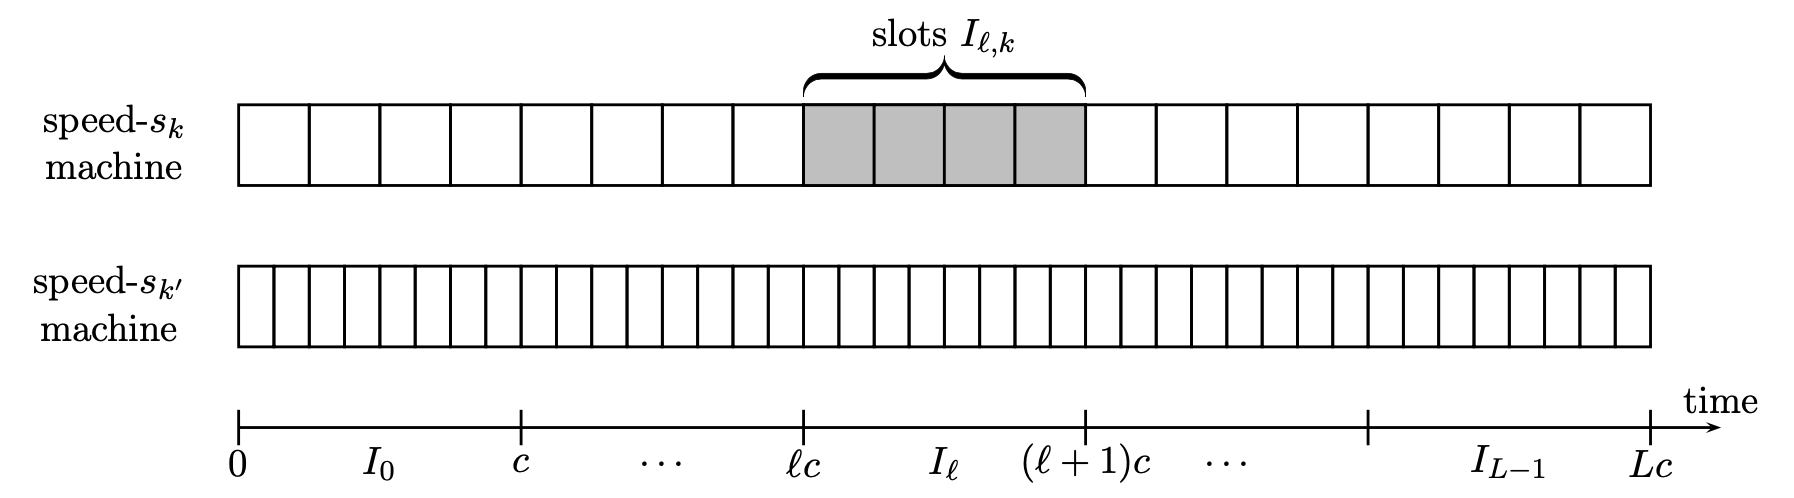
\includegraphics[width=15cm]{chapters/scheduling2/speed_slots}
%     \psset{xunit=0.7cm,yunit=0.8cm}
%     \begin{pspicture}(0,-0.5)(20,4.5)
%      \multido{\N=0+1}{20}{\rput[c](\N,3){\pspolygon(0,0)(1,0)(1,1)(0,1)}}
%      \multido{\N=8+1}{4}{\rput[c](\N,3){\pspolygon[fillcolor=lightgray,fillstyle=solid](0,0)(1,0)(1,1)(0,1)}}
%      \multido{\N=0.0+0.5}{40}{\rput[c](\N,1){\pspolygon(0,0)(0.5,0)(0.5,1)(0,1)}}
%      \psline{->}(0,0)(21,0) \rput[c](21,8pt){time}
%      \rput[r](-0.5,3.5){$\begin{array}{c} \textrm{speed-}s_k \\ \textrm{machine} \end{array}$}
%      \rput[r](-0.5,1.5){$\begin{array}{c} \textrm{speed-}s_{k'} \\ \textrm{machine} \end{array}$}
%      \psline(0,5pt)(0,-5pt) \rput[c](0,-10pt){$0$}
%      \psline(4,5pt)(4,-5pt) \rput[c](4,-10pt){$c$}
%      \psline(8,5pt)(8,-5pt) \rput[c](8,-10pt){$\ell c$}
%      \psline(12,5pt)(12,-5pt) \rput[c](12,-10pt){$(\ell+1)c$}
%      \psline(16,5pt)(16,-5pt) %\rput[c](12,-10pt){$(\ell+1)c$}
%      \psline(20,5pt)(20,-5pt) \rput[c](20,-10pt){$L c$}
%      \rput[c](2,-10pt){$I_0$}
%      \rput[c](6,-10pt){$\ldots$}
%      \rput[c](10,-10pt){$I_{\ell}$}
%      \rput[c](14,-10pt){$\ldots$}
%      \rput[c](18,-10pt){$I_{L-1}$}
     
%      \psbrace[rot=-90,ref=1C,nodesepB=-5pt,braceWidthInner=5pt,braceWidthOuter=5pt](12,4.1)(8,4.1){slots $I_{\ell,k}$}
%     \end{pspicture}
    \caption{Slots for different machine types.\label{fig:SlotsForMachineClasses}}
  \end{center}
  \end{figure}
  
  
  We construct the LP in two steps.
  First consider the variables
  \[
    x_{j,i,t} = \begin{cases} 1 & \textrm{if }j\textrm{ is scheduled on machine }i\textrm{ in time slot }t \in I_{*,k} \,, \\ 0 & \textrm{otherwise} \end{cases}
  \]
  for all $j \in J$, $k \in [M]$, $i \in [m_k]$, and $t \in I_{*,k}$.
  Let $K$ be the set of fractional solutions to the following linear system:
  \begin{eqnarray*}
    \sum_{k \in [M], i \in [m_k]} \sum_{t \in I_{*,k}} x_{j,i,t} &=& 1 \quad \forall j \in J \\
    \sum_{j \in J} x_{j,i,t} &\leq& 1 \quad \forall k \in [M] \;\; \forall i \in [m_k] \;\; \forall t \in I_{*,k} \\
    0 \leq x_{j,i,t} &\leq& 1 \quad \forall j \in J \; \forall k \in [M] \; \; \forall i \in [m_k] \; \forall t \in I_{*,k}
  \end{eqnarray*}
  
  
  We note that the assignment constraints are the set of equations 
  $\sum_{k \in [M], i \in [m_k]} \sum_{t \in I_{*,k}} x_{j,i,t} = 1$ for every $j \in J$.
  
  Next, we will use a lift $x \in \textsc{SA}_r(K)$, which contains in particular the variables
  $x_{(j_1,i_1,t_1),(j_2,i_2,t_2)}$ that provide the probability for the event that $j_1$ is scheduled at time $t_1$ on machine $i_1$ and
  $j_2$ is scheduled at time $t_2$ on machine $i_2$.
  We introduce more types of decision variables: 
  \begin{eqnarray*}
    y_{j_1,j_2,k} &=& \begin{cases} 1 & j_1\textrm{ and }j_2\textrm{ are scheduled on the same machine of type $k$ in the same interval,} \\ 0 & \textrm{otherwise,} \end{cases} \\
    y_{j_1,j_2} &=& \begin{cases} 1 & j_1\textrm{ and }j_2\textrm{ are scheduled on the same machine in the same interval,} \\ 0 & \textrm{otherwise,} \end{cases} \\
     C_j &=& \textrm{completion time of job }j.
  \end{eqnarray*}
  
  
  The LP relaxation is then as follows: 
  \begin{eqnarray*}
    \textrm{Minimize} & & \sum_{j \in J} w_j \cdot C_j  \quad \textsf{(LP)} \\
    y_{j_1,j_2,k} &=& \sum_{\ell \in \{ 0,\ldots,L-1\}}  \sum_{i \in [m_k]} \sum_{t_1 \in I_{\ell,k}} \sum_{t_2 \in I_{\ell,k}} x_{(j_1,i,t_1),(j_2,i,t_2)} \quad \forall j_1,j_2 \in J\; \forall k \in [M] \\
    y_{j_1,j_2} &=& \sum_{k}  y_{j_1,j_2,k}  \hspace{5.9cm} \forall j_1,j_2 \in J\\
    C_{j_2} &\geq& C_{j_1} + (1-y_{j_1,j_2}) \cdot c \hspace{4.3cm} \forall j_1 \prec j_2 \\
    C_j &=&  \sum_{k \in [M], i \in [m_k]} \sum_{t \in I_{*,k}} x_{j,i,t} \cdot t \hspace{3.7cm} \forall j \in J \\ 
    x &\in& SA_r(K)
  \end{eqnarray*}
  
  Following the discussion in Section~\ref{sec:SheraliAdamsHierarchy}, we know that for every job $j$, there is a
  distribution that we denote as $(\tilde{x},\tilde{y}) \sim \pazocal{D}(j^*)$ such that $\E[\tilde{x}_{j,i,t}] = x_{j,i,t}$
  and $\E[\tilde{y}_{j_1,j_2}] = y_{j_1,j_2}$ with $\tilde{x} \in SA_{r-1}(K)$ where job $j^*$ is integrally assigned and $(\tilde{x},\tilde{y})$ satisfies the first two constraints in $(\mathsf{LP})$.
  This is immediate for the $x$-part as $x \in SA_r(K)$, and follows for the $y$-variables as these  
  linear in the $x$-variables. 
  %In several proofs, we consider a solution drawn after conditioning on event. 
  %When we condition on a job $j$ being assigned integrally to a machine and time slot, we denote the corresponding solution and distribution as $(\tilde{x},\tilde{y}) \sim \pazocal{D}(j)$. 
  If $\pazocal{E}$ is an event, then we write $(\tilde{x},\tilde{y}) \sim \pazocal{D}(j^* \mid \pazocal{E})$ as the conditional distribution (conditioning on the event $\pazocal{E}$ occurring), see again Section~\ref{sec:SheraliAdamsHierarchy} for details.
  
  
  
  %#########LP Properties###################
  
  \subsection{Properties of the LP}
  \label{sec:LP-properties}
  
  We will now discuss some properties that are implied by the Sherali-Adams lift.
  The properties proved in this section, which we use crucially in our rounding algorithms, are the main technical contributions of this paper.
  
  \begin{lemma}\label{lem:Relmetric}
  Let $(x,y,C)$ be a solution to $(\mathsf{LP})$ with $r \geq 5$. Then $d(j_1,j_2) := 1-y_{j_1,j_2}$ is a semimetric.
  \end{lemma}
  This property was proven in \cite{DKRTZ20} for a special case of $s_k = 1$
  and is not hard to extend to our more general LP. From now on, the symbol $d$ as well as the quantity $\textrm{diam}( \cdot )$ will always refer to this particular semimetric. 
  For the special case of $s_k = 1$ for all $k$, one can also find a proof in \cite{DKRTZ20} that any set $U \subseteq J$ with $\textrm{diam}(U) \leq \frac{1}{2}$ has size $|U| \leq 2c$.
  While this is a obviously false for arbitrary speeds $s_k$, we can prove a similar claim: 
  %\begin{lemma}\label{lem:Rclustercapacity} % T: This lemma was not needed. 
  %For every $j_1 \in J$ and for every machine type $k \in [M]$, one has $\sum_{j_2 \in J} y_{j_1,j_2,k} \leq s_k \cdot c$.
  %\end{lemma}
  %The above lemmas are generalizations of the lemmas we proved for the identical machines case \cite{}, and we defer the proofs to appendix.
  \begin{lemma} \label{lem:BoundSumOfYj1j2kForFixedJ1}
  For $k \in [M]$ and $j_1 \in J$ one has $\sum_{j_2 \in J} y_{j_1,j_2,k} \leq s_k \cdot c \cdot \sum_{i \in [m_k]}\sum_{t}
  x_{j_1,i,t} \leq s_k \cdot c$.
  \end{lemma}
  \begin{proof}
    The second inequality is trivial as $\sum_{i \in [m_k]} \sum_{t} x_{j_1,i,t} \leq 1$, so we only justify the first inequality. 
  As we are proving a linear inequality, it suffices to show this for a fixed outcome $(\tilde{x},\tilde{y}) \sim \pazocal{D}(j_1)$ where job $j_1$ is assigned integrally. 
  If in $(\tilde{x},\tilde{y})$ the job $j_1$ is not assigned to a machine in $[m_k]$, then both sides are 0. 
  So suppose that $j_1$ is assigned to a machine $i_1 \in [m_k]$ and to interval $\ell_1$.
  Then indeed
  \[
  \sum_{j_2 \in J} \tilde{y}_{j_1,j_2,k} = \sum_{j_2 \in J} \sum_{t \in I_{\ell_1,k}} \tilde{x}_{j_2,i_1,t} \leq s_k c = s_k c \underbrace{\sum_{i \in [m_k]}\sum_{t} \tilde{x}_{j_1,i,t}}_{=1}
  \,.
  \]
  \end{proof}
  
  
  Lemmas~\ref{lem:RSmallNeighborhoodOfClosePoints} and \ref{lem:StrongerRSmallNeighborhoodOfClosePoints} are key technical insights  behind the algorithms for the related machines setting. They say that if one considers a set of jobs which are close to each other with respect to $d$,  then there exists a type $k^*$ such that we can schedule all the jobs in an interval of length $O(c)$ on a single machine of type $k^*$. Moreover, the LP also schedules a good fraction  of these jobs on the same machine type.
  These lemmas are important in assigning jobs to machine types in our algorithms.
  
  
  
  \begin{lemma}
  \label{lem:RSmallNeighborhoodOfClosePoints}
  Let $U \subseteq J$ be a non-empty subset of jobs with $\textrm{diam}(U) \leq \frac{1}{4}$. Then there exists a $k^* \in [M]$ such that
  \begin{enumerate*}
  \item[(i)] $|U| \leq O(1) \cdot s_{k^*} \cdot c$, and
  \item[(ii)] $\sum_{j \in U} \sum_{i \in [m_{k^*}]} \sum_t x_{j,i,t} \geq \Omega(\frac{1}{M}) \cdot |U|$.
  \end{enumerate*}
  \end{lemma}
  
  \begin{proof} 
  Let us sort the speed classes $[M]$ so that $s_1 \geq \ldots \geq s_M$ and abbreviate $z_{j,k} := \sum_{i \in [m_k]} \sum_t x_{j,i,t}$ as the fraction of job $j$ scheduled on class $k$.
  Moreover  let $\rho_{k} := \sum_{j \in U} z_{j,k}$ be the load of cluster $U$ on class $k$.
  We fix an arbitrary job $j^* \in U$. Let $k_{\textrm{median}} \in [M]$ be the median speed class for job $j^*$, meaning that $\sum_{k \leq k_{\textrm{median}}} z_{j^*,k} \geq \frac{1}{2}$ and $\sum_{k \geq k_{\textrm{median}}} z_{j^*,k} \geq \frac{1}{2}$. 
  We split the remaining proof into two separate claims. \\
  {\bf Claim I.} \emph{One has $|U| \leq  4 \cdot s_{k_{\textrm{median}}} \cdot c$.} \\
  {\bf Proof of Claim I.} First we observe that for every $j \in U$ we have $\sum_{k \geq k_{\textrm{median}}} y_{j^*,j,k} \geq \frac{1}{2}-d(j^*,j) \geq \frac{1}{4}$. 
  We use this to estimate
  \begin{eqnarray*}
  \frac{|U|}{4} &\leq&  \sum_{k \geq k_{\textrm{median}}}\sum_{j \in U} y_{j^*,j,k} \stackrel{\textrm{Lem~\ref{lem:BoundSumOfYj1j2kForFixedJ1}}}{\leq}
  \sum_{k \geq k_{\textrm{median}}} s_k c\sum_{i \in [m_k]}\sum_{t}
  x_{j^*,i,t} \\ &\leq& s_{k_{\textrm{median}}}c \underbrace{\sum_{k \geq
  k_{\textrm{median}}} \sum_{i \in [m_k]}\sum_t x_{j^*,i,t}}_{\leq 1} 
  \leq s_{k_{\textrm{median}}}c
  \end{eqnarray*}
  Rearranging gives $|U| \leq 4s_{k_{\textrm{median}}}c$ as claimed. \qed \\
  {\bf Claim II.} \emph{There is a class $k^* \in \{1,\ldots,k_{\textrm{median}}\}$ where $\rho_{k^*} \geq \frac{|U|}{4M}$.} \\
  {\bf Proof of Claim II.} For any job $j \in U$ we have $\sum_{k \leq k_{\textrm{median}}} z_{j,k} \geq (\sum_{k \leq k_{\textrm{median}}} z_{j^*,k}) - d(j,j^*) \geq \frac{1}{2} - \frac{1}{4} = \frac{1}{4}$.
  Hence $\sum_{k \leq k_{\textrm{median}}} \rho_k \geq \frac{|U|}{4}$.
  Then at least one index $k^* \in \{ 1,\ldots,k_{\textrm{median}}\}$ will have $\rho_{k^*} \geq \frac{|U|}{4M}$.
  \end{proof}
  
  %The above lemma guides in assigning clusters of jobs obtained via the CKR algorithm to machine types.
  While the above lemma is enough to obtain our approximation algorithm for  makespan on related machines, for the weighted completion time objective we need the following strengthening: if one considers a set of jobs which are {\em very} close to each other, then there exists a type $k^*$ such that we can schedule all the jobs in an interval of length $O(c)$ on a single machine of type $k^*$. 
  Moreover, the LP solution also schedules at least $\Omega(1/M)$ fraction of {\em every one of these jobs} on the same machine type.
  Recall that Lemma \ref{lem:RSmallNeighborhoodOfClosePoints} only satisfied this condition on average.
  
  % Recall that we use the notation $(\tilde{x},\tilde{y}) \sim \pazocal{D}(j^*)$ to obtain the distribution corresponding to the Sherali-Adams lift, where job $j^*$ is assigned integrally. 
  
  
  \begin{lemma}
  \label{lem:StrongerRSmallNeighborhoodOfClosePoints}
  Let $U \subseteq J$ be a non-empty set with $\textrm{diam}(U) \leq \frac{1}{8M}$ and abbreviate $z_{j,k} := \sum_{i \in [m_k]} \sum_{t} x_{j,i,t}$. Then
  \begin{enumerate*}
     \item[(i)] $|z_{j_1,k} - z_{j_2,k}| \leq \textrm{diam}(U) \leq
  \frac{1}{8M}$ for all $j_1,j_2 \in U$ and $k \in [M]$.
     \end{enumerate*}
     Moreover there are indices $\pi(U) \subseteq [M]$ such that
     \begin{enumerate}
     \item[(ii)] $z_{j,k} \geq \frac{1}{4M}$ for all $j \in U$ and $k \in \pi(U)$
     \item[(iii)] $\sum_{k \in \pi(U)} \min\{ z_{j,k} : j \in U\}
  \geq \frac{1}{2}$
     \item[(iv)] $|U| \leq 2 \cdot s_k \cdot c$ for all $k \in \pi(U)$.
     \end{enumerate}
  \end{lemma}
  
  
  \begin{proof}
  We prove the points in order.
  \begin{enumerate}
  \item[(i)] Actually we claim the stronger property of $|z_{j_1,k} - z_{j_2,k}| \leq d(j_1,j_2)$.
  Sample a distribution $(\tilde{x},\tilde{y}) \sim \pazocal{D}(j_1,j_2)$ and let $\sigma(j_1) \in [m]$ be the random variable that denotes the machine index with $\sum_t \tilde{x}_{j_1,\sigma(j_1),t}=1$ (similarly we define $\sigma(j_2)$). 
  Then we can see that
  \[
  |z_{j_1,k}-z_{j_2,k}| = |\Pr[\sigma(j_1) \in [m_k]] -
  \Pr[\sigma(j_2) \in [m_k]]| \leq |\Pr[\sigma(j_1) \neq \sigma(j_2)]|
  \leq d(j_1,j_2).
  \]
  \end{enumerate}
  Now we fix any job $j^* \in U$ and set $\pi(U) := \{ k \in [M] : z_{j^*,k} \geq \frac{1}{4M} \}$. 
  Then we continue the proof:
  \begin{enumerate}
  \item[(ii)] By (i) we know that for each $j \in U$ and $k \in \pi(U)$ we have $z_{j,k} \geq z_{j^*,k} - \frac{1}{8M} \geq \frac{1}{4M}$.
  \item[(iii)] We have
  
  \begin{eqnarray*}
  \sum_{k \in \pi(U)} \min\{ z_{j,k} : j \in U\} &\geq&
  \sum_{k \in \pi(U)} \Big(z_{j^*,k}-\frac{1}{8M}\Big) \\ &\geq&
  \underbrace{\sum_{k \in [M]} z_{j^*,k}}_{=1} - \sum_{k \in [M] \setminus
  \pi(U)} \underbrace{z_{j^*,k}}_{\leq 1/(4M)} - \frac{1}{8M}
  \underbrace{|\pi(U)|}_{\leq M} \geq \frac{1}{2}
  \end{eqnarray*}
  
  \item[(iv)] Fix a machine type $k \in \pi(U)$ and consider the event $\pazocal{E} := ``\sum_{i \in [m_k]}\sum_{t} \tilde{x}_{j^*,i,t}=1''$ (meaning the event that $j^*$ is assigned to a machine in class  $k$). 
  Note that $\Pr_{(\tilde{x},\tilde{y}) \sim \pazocal{D}(j^*)}[\pazocal{E}] = z_{j^*,k} \geq \frac{1}{4M}$. 
  %We study the conditional distribution  $(\tilde{x},\tilde{y}) \sim \pazocal{D}(j^* \mid \pazocal{E})$.
  Now, let $(\bar{x},\bar{y})$ be the Sherali-Adams lift (see Lemma~\ref{lem:SAconditioningOnGroupOfIndices}) conditioned on the event $\pazocal{E}$. Then trivially $\sum_{i \in [m_k]}\sum_t  \bar{x}_{j^*,i,t} = 1$. 
  As we have conditioned on an event with probability $z_{j^*,k} \geq \frac{1}{4M}$, the chance of other events cannot increase by more than a factor of $4M$ (see again Lemma~\ref{lem:SAconditioningOnGroupOfIndices}).
  In particular for $j \in U$ we have $1 - \bar{y}_{j^*,j} \leq 4M \cdot (1-y_{j^*,j}) = 4M \cdot d(j^*,j) \leq \frac{1}{2}$.
  As $\bar{y}_{j^*,j,k'} = 0$ for all $k' \neq k$ and $j \in U$ we can conclude that $\bar{y}_{j^*,j,k} \geq \frac{1}{2}$ for all $j \in U$.
  Finally by Lemma~\ref{lem:BoundSumOfYj1j2kForFixedJ1} we know that $\sum_{j \in J} \bar{y}_{j^*,j,k} \leq s_k c$ which then gives $|U| \leq 2s_kc$.
  \end{enumerate}
  \end{proof}
  
  As it is always the case when using the Sherali-Adams hierarchy in the context of approximation algorithms,
  it is a valid question how much of the power of the hierarchy is really needed. Some properties
  such as the triangle inequality from Lemma~\ref{lem:Relmetric} or the constraints from Lemma~\ref{lem:BoundSumOfYj1j2kForFixedJ1} could be enforced by simply adding them to the original LP. However at various places such as Lemmas~\ref{lem:StrongerRSmallNeighborhoodOfClosePoints}, \ref{lem:RAlphapointBound} and \ref{lem:RVolumeBound} our analysis makes heavily use of the local consistency provided by the hierarchy. It remains open whether there is a more efficient linear program, say only with the original
  variables $x_{i,j,t},y_{j_1,j_2},C_j$ that suffices.
  
  %#########Rounding Algorithm.###################
  \section{The Rounding Algorithm for $\Q \mid \Prec, p_j=1, c \mid \sum w_j C_j$}
  \label{sec:Rounding}
  
  
  In this section, we describe the rounding algorithm which proves our main technical result, Theorem~\ref{thm:LPcompletiontime}.
  We let $C_j^A$ denote the algorithm's completion time of job $j$.
  We denote $\Gamma^{-}(j)$ as the predecessors of $j$ and $\Gamma^+(j)$ as the successors, 
  and similarly $\Gamma^{-/+}(J') = \{ j \in J : \exists j' \in J' \textrm{ s.t. } j \in \Gamma^{-/+}(j') \}$. 
  
  \begin{theorem}
  \label{thm:LPcompletiontime}
  There is a polynomial-time randomized algorithm that,
  given a solution $(x,y,C)$ to (LP) for $r \geq 5$,
  produces a schedule with completion times 
  $\{C^A_j\}_{j \in J}$ such that $$\E[C^A_j] \leq O(M \cdot \log^2 n) \cdot C_j \leq O(\log ^3 n) \cdot C_j.$$
  \end{theorem}
  
  Before we describe our rounding algorithm, we set up some notation.
  Let $(x, y, C)$ be an optimal solution to the LP with $r \geq 5$.
  We partition the jobs based on their fractional completion times in the LP solution. 
  For any constant $a > 128$ set $\delta = \frac{1}{a \cdot M \cdot \log 2n }$. 
  Consider
  \begin{equation}
  J_0 := \left \{ j : C_j <  \delta  \cdot c \right \}
  \end{equation}
  
  and for $\gamma \geq 1$ define
  \begin{equation}
  \label{eq:jkdefinition}
  J_\gamma := \left \{ j : 2^{\gamma-1} \cdot \delta \cdot c \leq C_j <  2^{\gamma} \cdot \delta \cdot c \right \}
  \end{equation}
  
  
  \medskip
  Our rounding algorithm has the following steps:
  \begin{itemize}
  \item Schedule $J_0$ via the first batch scheduling algorithm given in Section \ref{sec:firstbatch}
  \item For $\gamma = 1, 2,\ldots$, schedule $J_\gamma$ via the intermediate scheduling algorithm  given in  Section \ref{sec:nextbatch}.
  \item Concatenate the schedules of $J_0, J_1, J_2, \ldots$.
  \end{itemize}
  
  
  We show that the expected completion time of every job in the above schedule satisfies Theorem \ref{thm:LPcompletiontime}. 
  We need the following scheduling subroutine for the rounding steps above.
  
  
  \begin{theorem} \label{thm:RelatedMakespan}
  Let $(x,y,C$) be a solution to the LP with $r \geq 5$ and let $T^* \in \mathbb{N}$.
  For some subset $J' \subset J$, suppose in the LP solution completion time $C_j \leq T^*$ for every job $j \in J'$.
  Then there is a randomized polynomial time algorithm that schedules all jobs such that $C^A_j \leq O(\log m \cdot \log n  \cdot T^*) + O(\log m \cdot c)$ for every job $j \in J'$.
   \end{theorem}
  
  Note that the above theorem immediately implies our result for the makespan minimization problem on related machines.
  We prove this theorem in Section \ref{sec:makespan}.
  
  
  \subsection{First Batch Scheduling}
  \label{sec:firstbatch}
  Here we give an algorithm for scheduling jobs in $J_0$.
  We define the \emph{$\alpha$-point} of job $j$ as the earliest time $t_j^*$ when 
  the LP solution has completed an $\alpha$-fraction of $j$. Formally,
  \begin{equation} \label{eq:RAlphaPoints}
    t^*_j := \min \left\{t' \in [T]:  \sum_{i=1}^{m}  \sum_{t \leq t'} x_{j,i,t} \geq \alpha \right\}.
  \end{equation}
  
  For $ \beta \leq 1/4M$, consider any subset $U \subseteq J$ with $\textrm{diam}(U) \leq \beta$.
  %$j^* \in J$, consider any $U := \{ j \in J \mid d(j,j^*) \leq \beta\}$.
  Let $\pi(U) \subseteq [M]$ denote the  indices of machine types that satisfy the conditions of Lemma \ref{lem:StrongerRSmallNeighborhoodOfClosePoints}.
  We use the same semimetric $d(j_1,j_2) := 1-y_{j_1,j_2}$ and schedule jobs in $J_0$ using the following algorithm.
  
  \begin{center}
   \fbox{
   \begin{minipage}{14cm}
    \textsc{First Batch Scheduling} \vspace{1mm} \hrule \vspace{1mm}
  \begin{enumerate*}
    \item[(1)] Run a CKR clustering on the semimetric space $(J_0,d)$ with parameter $\Delta := \frac{1}{100M}$ and let $V_1,\ldots,V_q$ be the clusters.
    \item[(2)] Let $V_{\ell}' := \{ j \in V_{\ell} \mid (\Gamma^-(j) \cap J_0) \subseteq V_{\ell}\}$ for $\ell = 1,\ldots,q$, and $J'_0 := \cup^{q}_{\ell = 1} V_{\ell}'$.
    \item[(3)] FOR $\ell = 1$ TO $q$ DO
          \begin{enumerate*}
            \item[(4)] Sample a machine type $k^*$ from the set $\pi(V'_\ell)$ with probability $\frac{\min \{z_{jk^*} : j \in V'_\ell \} }{\sum_{k \in \pi(V'_\ell)} \min \{z_{jk} : j \in V'_\ell \}}$.
            \item[(5)] Assign  $V'_\ell$ to a machine $i \in [m_{k^*}]$ with probability $\frac{1}{m_{k^*}}$.
           \end{enumerate*}
    \item [(6)] For a machine $i \in [m_k]$ of type $k$, let $J'_0(i,k)$ denote the set of jobs assigned to machine $i$.
    \item [(7)] For all $k$ and for all $i \in [m_k]$, schedule  $J'_0(i,k)$ in the increasing order of their $\alpha$-points for $\alpha = (1- \frac{1}{100M})$ as defined in Eq. (\ref{eq:RAlphaPoints}).
    \item[(8)] Insert a gap of $c$ time slots.
    \item[(9)] Let $J''_0 := J_0 \setminus J'_0$ be the set of jobs that did not get scheduled in steps (1) - (5). Use Theorem   \ref{thm:RelatedMakespan} to schedule $J''_0$.
    \end{enumerate*}
    \end{minipage}}
  \end{center}
  
  We now argue that expected completion time of a job $j$ in above algorithm is comparable to its LP cost.
  First we focus on bounding the completion time of jobs in $J'_0$.
  We need the following crucial lemma.
  
  \begin{lemma} 
  \label{lem:RAlphapointBound}
  %Let $\alpha = 1/100M$ be a small enough constant, and
  Let $U \subseteq J$ be a set of jobs  with $\textrm{diam}(U) \leq \frac{1}{100M}$ w.r.t. distance $d$. 
  For every job $j \in U$,  define $t_j^*$ as in Eq~\eqref{eq:RAlphaPoints}. 
  For $\theta > 0$, consider the set of jobs $U^* := \{ j \in U: t_j^* < \theta \} $ with $\alpha$-point less than $\theta$.  
  Then $|U^*| \leq 2 \cdot s_{k^*} \cdot \theta$ for any $k^* \in \pi(U)$.
   \end{lemma}
  
  The lemma formalizes the intuition that as the jobs in $U^*$ are very close to each other, it must be the case that the LP schedules all of them on the same machine.
  As a good fraction of each of these jobs are scheduled in the interval of length $\theta$ there cannot be too many of them.
  
  
  \begin{proof}
  We prove the lemma by contradiction.  Consider a set $U^*$ that violates the conditions in the lemma and fix a job $j^* \in U^*$.
  Let $k^* \in \pi(U)$.
  Then we have
    \begin{align*}
  (A) \;\; \sum_{j \in U^*} \sum_{i \in [m]} \sum_{t > \theta} x_{j,i,t}  < \frac{1}{100M} \cdot |U^*|, \quad &(B) \;\; \sum_{j \in U^*} y_{j,j^*} \geq \Big(1-\frac{1}{100M}\Big)|U^*|,\\ 
   \quad  &(C) \;\; \sum_{i \in [m_{k^*}]} \sum_{t \leq \theta} x_{j^*,i,t} \geq \frac{1}{5M}.
    \end{align*}
  where $(A)$ follows from the definition of $\alpha$-point of jobs, $(C)$ follows from  $\sum_{i \in [m_{k^*}]} \sum_{t=1}^{\theta} x_{j^*,i,t} \geq 1/4M - 1/100M > 1/5 M$, and
  $(B)$ follows from $\textrm{diam}(U^*) \leq \textrm{diam}(U) \leq \frac{1}{100M}$.
  Now we appeal to the properties of the Sherali-Adams hierarchy.
  Consider the event $\pazocal{E} := "\sum_{i \in [m_{k^*}]} \sum_{t \leq \theta} x_{j^*,i,t} = 1"$
  and note that from $(C)$ we know that the probability of the event $\pazocal{E}$ is at least $\frac{1}{5M}$.
  Now let $(\bar{x},\bar{y})$ be the Sherali-Adams lift with $\bar{x} \in SA_{r-1}(K)$ conditioned on this event, see Lemma~\ref{lem:SAconditioningOnGroupOfIndices} for details.
  In particular one has $\sum_{i \in [m_{k^*}]} \sum_{t \leq \theta} \bar{x}_{j^*,i,t} = 1$, meaning that the LP solution
  $(\bar{x},\bar{y})$ schedules $j^*$ fully on machines of class $k^*$ and until time $\theta$. 
  
  %We know that there is a distribution  $(\tilde{x},\tilde{y}) \sim \pazocal{D}(j^*)$ so that $\E[\tilde{x}_{j,i,t}] = x_{j,i,t}$ and $\E[\tilde{y}_{j_1,j_2}]=y_{j_1,j_2}$ while the variables involving job $j^*$ are integral, i.e. $\tilde{x}_{j^*,i,t} \in \{ 0,1\}$.
  %Now consider the conditional distribution  $(\tilde{x},\tilde{y}) \sim \pazocal{D}(j^* \mid \pazocal{E})$. 
  As we have conditioned on an event of probability at least $\frac{1}{5M}$, the probabilities of other events cannot increase by more than a factor of $5M$ (see the ``moreover'' part in Lemma~\ref{lem:SAconditioningOnGroupOfIndices}). 
  In particular for $j \in U$ we have $1 - \bar{y}_{j^*,j} \leq 5M \cdot (1-y_{j^*,j}) = 5M \cdot d(j^*,j) \leq \frac{1}{10}$.
  Similarly, $\sum_{j \in U^*} \sum_{i \in [m]} \sum_{t > \theta} \bar{x}_{j,i,t}  \leq 5M \cdot (\sum_{j \in U^*} \sum_{i \in [m]} \sum_{t > \theta} x_{j,i,t}) \leq 5M \cdot \frac{1}{100M} \cdot |U^*| \leq \frac{|U^*|}{10}$.
  Therefore we have 
    \[
  (A') \;\; \sum_{j \in U^*} \sum_{i \in [m_{k^*}]} \sum_{t > \theta} \bar{x}_{j,i,t}  \leq \frac{|U^*|}{10}, \quad (B')  \sum_{j \in U^*} \bar{y}_{j,j^*} \geq \frac{9}{10} \cdot |U^*|, \quad   (C') \sum_{i \in [m_{k^*}]} \sum_{t\leq \theta} \bar{x}_{j^*,i,t} = 1.
  \]
  Then by Markov's inequality there exists an outcome  $(\tilde{x},\tilde{y}) \sim \pazocal{D}_{\bar{y}}(j^*)$ where the job $j^*$ is integrally assigned and
    \[
  (A'') \;\; \sum_{j \in U^*} \sum_{i \in [m_{k^*}]} \sum_{t > \theta} \tilde{x}_{j,i,t}  \leq \frac{|U^*|}{5}, \quad (B'')  \sum_{j \in U^*} \tilde{y}_{j,j^*} \geq \frac{4}{5} \cdot |U^*|, \quad   (C'') \sum_{i \in [m_{k^*}]} \sum_{t \leq \theta} \tilde{x}_{j^*,i,t} = 1.
  \]
  We fix that outcome and let $i^* \in [m_{k^*}],t^* \in \{ 1,\ldots,\theta\}$ be the indices with $\tilde{x}_{j^*,i^*,t^*}=1$. Let $\ell^*$ be the interval index such that $t^* \in I_{\ell^*,k^*}$. 
  Then
  \begin{eqnarray*}
    \frac{4}{5} \cdot |U^*| &\stackrel{(B'')}{\leq}& \sum_{j \in U^*} \tilde{y}_{j,j^*} \stackrel{LP}{=} \sum_{j \in U^*} \sum_{\ell \in \{ 0,\ldots,L-1\}} \sum_{k} \sum_{i \in [m_k]} \sum_{t_1 \in I_{\ell,k}} \sum_{t_2 \in I_{\ell,k}} \tilde{x}_{(j,i,t_1),(j^*,i,t_2)} \\ 
    &\leq& \sum_{j \in U^*}\sum_{t \in I_{\ell^*,k^*}}\tilde{x}_{j,i^*,t}
    = \underbrace{\sum_{j \in U^*} \sum_{t \in I_{\ell^*,k^*}: t \leq \theta} \tilde{x}_{j,i^*,t}}_{\leq s_{k^*} \cdot \theta\textrm{ by LP}} + \underbrace{\sum_{j \in U^*} \sum_{t \in I_{\ell^*,k^*}:t > \theta^*} \tilde{x}_{j,i^*t}}_{\leq \frac{1}{5} \cdot |U^*| \textrm{ by }(A'')} \\
    &\leq& s_{k^*} \cdot \theta + \frac{|U^*|}{5}
  \end{eqnarray*}
  Rearranging gives $|U^*| \leq \frac{5}{3} \cdot s_{k^*} \cdot \theta^*$, which is a contradiction.
  \end{proof}
  
  
  \begin{lemma}
  \label{lem:RVolumeBound}
  Let $\theta > 0$ and $i$ be any machine of type $k$. Then with high probability $1-1/n^{100}$ it holds that
  $$
  | \{ j \in J'_0(i,k) : t^*_j \leq   \theta \} | \leq O\Big(\frac{\log n}{\log \log n} \cdot s_k \cdot \theta\Big)
  $$
   \end{lemma}
  \begin{proof}
  Fix $\theta^* > 0$ and any machine $i^*$ of type $k$. 
  Consider any outcome of the clustering itself. 
  The randomness needed for the lemma is only over the assignment in step (3)-(5) of the algorithm. We define the following random variables. Let
  \[
  X_{\ell}= \begin{cases}  | \{ j \in V'_{\ell} : t^*_j \leq   \theta^* \} | &\textrm{if } V'_{\ell} \textrm{ is assigned to machine} \hspace{1mm} i^* \hspace{1mm}   \textrm{of type} \hspace{1mm} k \hspace{1mm} \textrm{by our algorithm,} 
  \\ 0 & \textrm{otherwise} 
  \end{cases}
  \]
  and abbreviate $X = \sum^{q}_{\ell = 1} X_\ell$. Note the random variables $X_{1},\ldots,X_q$ are independent and $X = | \{ j \in J'_0(i^*,k) : t^*_j \leq   \theta^* \} |$.
  From Lemma \ref{lem:RAlphapointBound} we know that $X_\ell \leq 2s_k \cdot \theta^*$ for all $\ell$.
  
  Next, we estimate $\E[X]$. Recall that the algorithm uses the indices $\pi(V_{\ell}') \subseteq [M]$ from Lemma~\ref{lem:StrongerRSmallNeighborhoodOfClosePoints} 
  which in particular satisfy $z_{j,k} \geq \frac{1}{4M}$ and $|z_{j,k}-z_{j',k}| \leq \frac{1}{8M}$ whenever $j,j' \in V_{\ell}'$ with $k \in \pi(V_{\ell}')$.
  Abbreviate
  \[
    \mu_{\ell,k} := \begin{cases} \min\{ z_{j,k} : j \in V_{\ell}' \} & \textrm{if }k \in \pi(V_{\ell}') \\
      0 & \textrm{otherwise.} \end{cases}
  \]
  Recall that for every $\ell$ we have $\sum_{k \in [M]} \mu_{\ell,k} \geq 1/2$. We prove two technical claims that we need for our analysis: \\
  {\bf Claim I.} \emph{For any $\ell$ and $k$ and $j \in V_{\ell}'$ one has $\mu_{\ell,k} \leq 2z_{j,k}$.} \\
  {\bf Proof of Claim.} If $k \notin \pi(V_{\ell}')$ then the left hand side is 0, so suppose  $k \in \pi(V_{\ell}')$. Then $\mu_{\ell,k} = \min\{ z_{j',k} : j' \in V_{\ell}'\} \leq z_{j,k} + \frac{1}{8M} \leq 2z_{j,k}$. \qed \\
  {\bf Claim II.} \emph{For $j \in V_{\ell}'$ with $t_j^* \leq \theta^*$ and $k \in \pi(V_{\ell}')$ one has $z_{j,k} \leq 2 \sum_{i \in [m_k]} \sum_{t \in I_{*,k}: t \leq \theta^*} x_{j,i,t}$.}
  {\bf Proof of Claim II.} Since $k \in \pi(V_{\ell}')$ we know that $z_{j,k} \geq \frac{1}{4M}$.
  We consider the distribution $(\tilde{x},\tilde{y}) \sim \pazocal{D}(j)$ and denote $\tilde{i}$ and $\tilde{t}$ as the random indices so that $\tilde{x}_{j,\tilde{i},\tilde{t}}=1$. Then $\Pr[\tilde{i} \in [m_k]] = z_{j,k}$ and $\Pr[\tilde{t} > \theta^*] = \sum_{k \in [M]} \sum_{i \in [m_k]} \sum_{t \in I_{*,k}: t > \theta^*} x_{j,i,t} \leq \frac{1}{100M}$ by the definition of $\alpha$-points and the assumption $t_{j}^* \leq \theta^*$. Then
  \begin{eqnarray*}
    \sum_{i \in [m_k]} \sum_{t \in I_{*,k}: t \leq \theta^*} x_{j,i,t} &=& \Pr\big[\tilde{i} \in [m_k]\textrm{ and }\tilde{t} \leq \theta^*\big] \\
    &\geq&  \Pr\big[\tilde{i} \in [m_k]\big] - \Pr\big[\tilde{t} > \theta^*\big] \\
    &\geq& z_{j,k} - \frac{1}{100M} \geq \frac{1}{2}z_{j,k} \quad \quad \qed
  \end{eqnarray*}
  
  Now we can bound the expectation of our random variable as
  \begin{eqnarray*}
    \E[X] &=& \frac{1}{m_k} \sum_{\ell=1}^q \Pr\big[V_{\ell}'\textrm{ assigned to class }k\big] \cdot |\{j \in V_{\ell}': t_j^* \leq \theta^*\}| \\
          &=& \frac{1}{m_k} \sum_{\ell=1}^q \frac{\mu_{\ell,k}}{\sum_{k'} \mu_{\ell,k'}} \cdot |\{j \in V_{\ell}': t_j^* \leq \theta^*\}| \\
    &\stackrel{\textrm{Claim I}}{\leq}& \frac{4}{m_k} \sum_{\ell: k \in \pi(V_{\ell}')} \sum_{j \in V_{\ell}': t_j^* \leq \theta^*} z_{j,k} \\
          &\stackrel{\textrm{Claim II}}{\leq}& \frac{8}{m_k} \sum_{\ell: k \in \pi(V_{\ell}')} \sum_{j \in V_{\ell}': t_j^* \leq \theta^*} \sum_{i \in [m_k]} \sum_{t \in I_{*,k}: t \leq \theta^*} x_{j,i,t} \\
   &\leq& \frac{8}{m_k} \sum_{i \in [m_k]} \sum_{t \in I_{*,k}: t \leq \theta^*} \underbrace{\sum_{j \in J_0'}  x_{j,i,t}}_{\leq 1\textrm{ by }(\mathsf{LP})} \leq 8 \cdot |\{ t \in I_{*,k}: t \leq \theta^*\}| \leq 8s_k \cdot \theta^*
  \end{eqnarray*}
  Here we also have used that $\sum_{k' \in [M]} \mu_{\ell,k'} \geq \frac{1}{2}$. 
  As $X$ is sum of independent random variables $X_\ell$ each of which is bounded by $O(s_k \cdot \theta^*)$, we apply the Chernoff bound from Lemma~\ref{lem:ChernoffBound} and obtain that $\Pr[X > C' \cdot \frac{\log n}{\log \log n} \cdot s_k \theta^*] \leq 1/n^{1000}$ for some constant $C'>0$.
  To complete the lemma, we simply do a union bound over all possible values of $\theta^*$ and $i$. The number of machines is $m \leq n$ and the number of relevant $\theta^*$'s in the time horizon is bounded by $\sum_{k \in [M]} |I_{*,k}| \leq M \cdot 2n$.
  \end{proof}
  % \begin{proof}
  % Fix $\theta^* \in \mathbb{N}$ and any machine $i^*$ of type $k$. \rem{T: Actually $\theta$ would be over all relevant times, but they do not need to be integer. }
  % Consider any outcome of the clustering itself. 
  % The randomness needed for the lemma is only over the assignment in step (3)-(5) of the algorithm. We define the following random variables. Let
  % \[
  % X_{\ell}= \begin{cases}  | \{ j \in V'_{\ell} : t^*_j \leq   \theta^* \} | &\textrm{if } V'_{\ell} \textrm{ is assigned to machine} \hspace{1mm} i^* \hspace{1mm}   \textrm{of type} \hspace{1mm} k \hspace{1mm} \textrm{by our algorithm,} 
  % \\ 0 & \textrm{otherwise} 
  % \end{cases}
  % \]
  % and abbreviate $X = \sum^{q}_{\ell = 1} X_\ell$. Note the random variables $X_{1},\ldots,X_q$ are independent and $X = | \{ j \in J'_0(i^*,k) : t^*_j \leq   \theta^* \} |$.
  % From Lemma \ref{lem:RAlphapointBound} we know that $X_\ell \leq 2s_k \cdot \theta^*$ for all $\ell$.
  
  % Let $ V^*$ be the set of all clusters that are assigned to machines of type $k$ by our algorithm,
  % and define $J_{\theta^*}(k) := \{j \in V^*:  t^*_j \leq \theta^* \}$.  
  % From the capacity constraints of the LP we know that $\sum_{j \in J_\theta^*(k)} z_{jk} \leq m_k \cdot s_k \cdot \theta^*$. \rem{T: This is not right mathematically. Due to the change in the algorithm, $V^*$ is a random set and $J_{\theta^*}(k)$. Then  $\sum_{j \in J_\theta^*(k)} z_{jk} \leq m_k \cdot s_k \cdot \theta^*$ isn't true (it might hold in expectation)}
  
  % Our algorithm assigns a cluster $V'_{\ell}$ to the machine $i^*$ if it satisfies the conditions of  Lemma \ref{lem:StrongerRSmallNeighborhoodOfClosePoints}. 
  % Then, $V'_{\ell}$ is assigned to $i^*$ with probability
  % $$
  % \frac{1}{m_k} \cdot \frac{\min \{z_{jk} : j \in V'_\ell \} }{\sum_{j \in V'_\ell} \min \{ z_{jk} : j \in V'_\ell \}} \leq \frac{1}{m_k}  \cdot 2  \cdot \min \{z_{jk} : j \in V'_\ell \}
  % $$
  % This further implies that a job $j \in J_\theta^*(k)$ is assigned to the machine $i^*$ with probability at most $z_{jk}/m_k$.
  % Now we can bound the expectation of random variable $X$. Consider,
  % $$
  % \E[X] =  \sum_{j \in J_\theta^*(k)} \textrm{Pr [$j$ is assigned to $i^*$]} \leq  \frac{2}{m_k} \cdot \sum_{j \in J_\theta^*(k)} z_{jk} = \frac{2}{m_k} \cdot  (m_k \cdot s_k \cdot \theta^*) \leq 2s_k \cdot \theta^* 
  % $$
  % As $X$ is sum of independent random variables $X_\ell$ each of which is bounded by $O(s_k \cdot c)$ by  Lemma \ref{lem:RAlphapointBound}, we apply the Chernoff bound from Lemma~\ref{lem:ChernoffBound} to argue that $\Pr[X > C' \cdot \frac{\log n}{\log \log n} \cdot s_k c] \leq 1/n^{1000}$ for some constant $C'>0$.
  % To complete the lemma, we simply do a union bound over all possible values of $\theta$ and $i$, both of which are bounded by $O(n)$. \rem{T: This has to be for all possibly relevant times and the upperbound that I see is $\sum_k |I_{0,k}| \leq c\sum_k s_k$. This isn't quite linear in $n$.}
  % \end{proof}
  
  
  \begin{lemma}
  \label{lem:completiontimeJ'_0}
  For every job $j \in J'_0$, with high probability, the completion time of $j$ in our schedule $C^{A}_j \leq O( M \cdot \frac{\log n}{\log \log n} \cdot C_j)$.
  \end{lemma}
  \begin{proof}
  Fix a job $j^* \in J'_0$, and suppose job $j^*$ is scheduled on machine $i$ of type $k$ in our schedule.
  From Lemma \ref{lem:RVolumeBound}, there are at most $O( \frac{\log n}{\log \log n} \cdot s_k \cdot t^*_{j^*})$ jobs whose $t^*_j \leq t^*_{j^*}$.
  Therefore, the completion time is  $C^A_{j^*} \leq O(\frac{\log n}{\log \log n} \cdot t^*_{j^*})$.
  Note that in the LP solution at least an $\frac{1}{100M}$-fraction of $j^*$ was scheduled at or after $t^*_{j^*}$.
  Hence, $C_j \geq \frac{1}{100M} \cdot t^*_{j^*}$.
  Putting things together we conclude  $C^{A}_j \leq O(\frac{\log n}{\log \log n} \cdot t_{j^*}^*) \leq O( M \cdot \frac{\log n}{\log \log n} \cdot C_j)$.
  \end{proof}
  
  
  
  Now we focus on bounding the completion time of jobs in $J''_0$. 
  
  \begin{lemma}
  \label{lem:completiontimeJ''_0}
  For every job $j \in J''_0$, the completion time of $j$ in our schedule $C^{A}_j \leq O( \log n \cdot c)$.
  \end{lemma}
  \begin{proof}
  From the definition of set $J_0$, for all $j \in J''_0$ the completion time $C_j \leq c \cdot \delta$ in the LP solution.
  This implies that at least a 1/2-fraction of every job $j \in J''_0$ is scheduled in the interval $[0, 2c \cdot \delta]$ in the LP solution.
  We take the LP solution restricted to $J''_0$ in the interval $[0, c \cdot \delta]$, and  invoke Theorem \ref{thm:RelatedMakespan} to construct a schedule of jobs $J''_0$.
  Theorem \ref{thm:RelatedMakespan} guarantees that every job  $j \in J''_0$ is scheduled in an interval of length at most $2c \cdot \delta \cdot (\log m \cdot \log n + M^2) + O(\log m \cdot c) = O(\log m \cdot c)$ from our choice of $\delta$.
  To complete the proof, it remains to account for the increase in completion time caused by jobs in  $J'_0$ as 
  our algorithm schedules $J''_0$ after scheduling jobs in $J'_0$.
  However, from Lemma \ref{lem:completiontimeJ'_0} every job in $J'_0$ has completion time at most $O(\log n \cdot c)$.
  Thus the lemma follows.
  \end{proof}
  
  \begin{lemma}\label{l:notin}
  For any job $j_1 \in J_0$, the probability that $j_1 \in J''_0$  is at most  $O(M \cdot \log n  \cdot \frac{C_{j_1}}{c})$.
  \end{lemma}
  \begin{proof}
    Consider the set $U := \{ j_1 \} \cup (\Gamma^{-}(j_1) \cap J_0)$ of $j_1$ and its ancestors. If $j_0 \prec j_1$, then $0 \leq C_{j_0} + c \cdot d(j_0,j_1) \leq C_{j_1}$ by the LP constraints and so $d(j_0,j_1) \leq \frac{C_{j_1}}{c}$.
    Then the diameter of $U$ with respect to semimetric $d$ is bounded by $2C_{j_1}/c$ and hence by Theorem~\ref{thm:ProbUSeperatedByClustering}.(b) the probability that $U$ is separated is bounded by $\ln(2n) \cdot \frac{4 \textrm{diam}(U)}{\Delta} \leq O(M \cdot \log n  \cdot \frac{C_{j_1}}{c})$.
  \end{proof}
  
  We can now bound the expected completion time of every job in $J_0$.
  \begin{lemma}
  \label{lem:completiontimeJ0}
  For every job $j \in J_0, \E[C^A_j] \leq O(M \cdot \log^2 n ) \cdot C_j$.
  \end{lemma}
  \begin{proof} 
  Fix a job $j_1 \in J_0$ and consider
  \begin{eqnarray*}
  \E[C^A_{j_1}]  &=& \E[C^A_{j_1} | (j_1 \in J'_0)] \cdot \text{Pr}[ (j_1  \in J'_0)] + \E[C^A_{j_1} | (j_1  \in J''_0)] \cdot \text{Pr}[ (j_1 \in J''_0)]  \\
  &\stackrel{(*)}{\leq}& O\Big( M \cdot \frac{\log n}{\log \log n} \cdot C_{j_1}\Big) +  O\Big(M \cdot \log n \cdot \frac{C_{j_1}}{c}\Big) \cdot O( \log n \cdot c)   \\
  &\leq& O(M \cdot \log^2 n) \cdot C_{j_1}, 
  \end{eqnarray*}
  where (*) follows from Lemmas  \ref{lem:completiontimeJ'_0}, \ref{lem:completiontimeJ''_0}, \ref{l:notin}.
  \end{proof}
  We also note the following simple consequence of previous lemmas:
  
  \begin{lemma}
  \label{lem:makespanofJ0}
  For every job $j \in J_0$, $C_j \leq O(\log n \cdot c)$.  In other words,  the makespan of our schedule for $J_0$ is at most $O(\log n \cdot c)$.
  \end{lemma}
  
  
  \subsection{Intermediate Batch Scheduling}
  \label{sec:nextbatch}
  Now we describe our algorithm to schedule jobs in the set $J_\gamma$ for $\gamma > 0$, which is  similar to that of scheduling jobs in $J''_0$.
  Recall that from the definition of set $J_\gamma$ in Eq. (\ref{eq:jkdefinition}), $2^{\gamma-1} \delta \cdot c  < C_j \leq  2^\gamma \delta \cdot c$ in the LP solution.
  We take the LP solution restricted to $J_\gamma$ in the interval $[0, 2^\gamma \delta \cdot c]$, and  invoke Theorem \ref{thm:RelatedMakespan} to construct a schedule of jobs $J_\gamma$.
  Theorem \ref{thm:RelatedMakespan} ensures that every job  $j \in J_\gamma$  is scheduled in an interval of length at most $O(2^\gamma \delta \cdot c \cdot \log m \cdot \log n) + O(\log n \cdot c)$. 
  As a consequence, we obtain the following lemma.
  \begin{lemma}
  \label{lem:intermediate}
  Fix any $\gamma^* \geq 0$. For every $j \in J_{\gamma^*}$, $C^A_j \leq O(2^{\gamma^*} \cdot \delta \cdot \log m \cdot \log n) + O(\gamma^* \cdot \log n \cdot c)$.
  \end{lemma}
  \begin{proof} 
  For $\gamma = 0, 1, \ldots$, let $\pazocal{S}(J_\gamma)$ denote the schedule of jobs in the set $J_\gamma$.
  Our final schedule $\pazocal{S}$ is simply a concatenation of schedules $\pazocal{S}(J_0), \pazocal{S}(J_1), \ldots$, while inserting $c$ empty time slots between  $\pazocal{S}(J_\gamma)$ and $ \pazocal{S}(J_{\gamma+1})$.
  Let $T_{\gamma}$ denote the makespan of $\pazocal{S}(J_\gamma)$.
  From Lemma \ref{lem:makespanofJ0} and Theorem \ref{thm:RelatedMakespan}, $T_{\gamma} \leq O(2^\gamma \cdot  \delta \cdot c \cdot \log m \cdot \log n ) + O(\log n \cdot c)$.
  Fix the job $j^* \in J_{\gamma^*}$ with the highest completion time in $\pazocal{S}$.
  We can bound the completion time of $j^*$ as
  
  \begin{eqnarray*}
  C^A_{j^*} &\leq& \sum^{\gamma^*}_{\gamma = 0} T_{\gamma} \leq  O(\gamma^* \cdot \log n \cdot c) + \sum^{\gamma^*}_{\gamma = 1} O(2^\gamma \cdot \delta \cdot c \cdot \log m \cdot \log n) \\
  &\leq& O(\gamma^* \cdot \log n \cdot c) + O(2^{\gamma^*} \cdot \delta \cdot c \cdot \log m \cdot \log n)
  \end{eqnarray*}
  which completes the proof.
  \end{proof}
  
  We finish the proof of main theorem for the weighted sum of completion times of jobs.
  
  \begin{proof} [Proof of Theorem \ref{thm:LPcompletiontime}]
  For every job $j \in J_0$, from Lemma \ref{lem:completiontimeJ0},  we have $\E[C^A_j] \leq O(M \cdot \log^2 n) \cdot C_j$.
  From the previous Lemma \ref{lem:intermediate}, for $\gamma  > 0$ and $j \in J_{\gamma }$ we have, $C^A_j \leq O(\gamma \cdot \log n \cdot c) + O(2^{\gamma } \cdot \delta \cdot c \cdot \log m \cdot \log n )$.
  On the other hand,  for every $j \in J_{\gamma}$, by definition, $C_j >  2^{\gamma} \cdot \delta \cdot c$.
  Thus, $C^A_j \leq  O(M \cdot \log^2 n) \cdot C_j$.
  \end{proof}
  
  
  %****************
  
  \section{Proof of Theorem \ref{thm:RelatedMakespan}}
  \label{sec:makespan}
  
  Recall that we are given a subset of jobs $J' \subseteq J$, and a solution $(x,y,C)$ to the LP with $r \geq 5$ and  $T \in \mathbb{N}$.
  It is promised that in  $(x,y,C)$, the completion times satisfy $C_j \leq T$ for every job $j \in J'$.
  Then there is a randomized polynomial time algorithm that schedules all jobs such that $C_j^A \leq O(\log m  \cdot \log n  \cdot T) + O(\log m \cdot c)$ for every job $j \in J'$. 
  %\rem{T: I added $C_j^A$ for the completion time of our algo.}
  
  \subsection{Main Scheduling Subroutine}
  \label{subsec:singlebatchrelated}
  
  The following lemma is the main scheduling subroutine towards proving Theorem \ref{thm:RelatedMakespan}. 
  
  \begin{lemma} \label{lem:RSchedulingOneIntervalViaCKR}
  Let $C^* \geq 0$ and $\delta = 1/64\log(2n)$. 
  Consider the set $J^* \subseteq \{ j \in J' \mid C^* \leq C_j \leq C^*+\delta \cdot c \}$.
  Then there is a randomized rounding procedure that finds a subset $J^{**} \subseteq J^*$,
  a partition of $J^{**}$ into $J^{**} = \cup_{k=1}^{M} J^{**(k)}$ where $J^{**(k)}$ are jobs assigned to machines of type $k$,
  and a schedule for $J^{**}$ in an interval of length at most $5c+\sum_k \frac{|J^{**(k)}|}{s_k \cdot m_k}$ such that every job $j \in J^*$
  is scheduled with probability at least $\frac{1}{2}$.
  \end{lemma}
  
  
  The rounding algorithm to prove the above lemma is the following:
  
  \begin{center}
  \fbox{
  \begin{minipage}{14cm}
    \textsc{Scheduling a Single Batch on Related Machines} \vspace{1mm} \hrule \vspace{1mm}
  \begin{enumerate*}
    \item[(1)] Run a CKR clustering on the semimetric space $(J^*,d)$ with parameter $\Delta := \frac{1}{4}$ and let $V_1,\ldots,V_q$ be the clusters.
    \item[(2)] Let $V_{\ell}' := \{ j \in V_{\ell} \mid \Gamma^-(j) \cap J^* \subseteq V_{\ell}\}$ for $\ell = 1,\ldots,q$.
    \item[(3)] For all $\ell=1,\ldots,q$, assign the jobs in $V_{\ell}'$ to type $k^*$ satisfying the conditions in Lemma \ref{lem:RSmallNeighborhoodOfClosePoints}.
    \item[(4)] For all $\ell=1,\ldots,q$, if $V_{\ell}'$ is assigned to type $k^*$, assign all jobs in $V_{\ell}'$ to the machine of type $k^*$ which has the least load (breaking ties arbitrarily). 
    \end{enumerate*}
     \end{minipage}}
  \end{center}
  
  We prove few lemmas that will be helpful in proving the desired properties of the algorithm.
  The first lemma shows that the clusters produced by the algorithm are not too large.
  
  \begin{lemma}
      \label{lem:RClusterSize}
  For all $\ell=1,\ldots,q$, one has $|V_{\ell}'| \leq O(s_{k^*}c)$. Here, $k^*$ is the machine type that $V_{\ell}'$ is assigned in our algorithm. Thus, it takes $O(c)$ time to process all jobs in $V_{\ell}'$. 
  \end{lemma}
  \begin{proof}
    We know by Theorem~\ref{thm:ProbUSeperatedByClustering} that $\textrm{diam}(V_{\ell}') \leq \textrm{diam}(V_{\ell}) \leq \Delta \le \frac{1}{4}$.
    The lemma follows by Lemma~\ref{lem:RSmallNeighborhoodOfClosePoints} and by our choice of $k^*$. 
  \end{proof}
  
  Further it is easy to see that the clusters respect precedence constraints.
  \begin{lemma}
  \label{lem:ClusterIndependence}
  The solution $V_{1}',\ldots,V_{q}'$ is feasible in the sense that jobs on different machines do not have precedence constraints.
  \end{lemma}
  \begin{proof}
    Consider jobs processed on different machines, say (after reindexing) $j_1 \in V_{1}'$ and $j_2 \in V_2'$.
     If $j_1 \prec j_2$ then we did \emph{not} have $\Gamma^-(j_2) \subseteq V_2'$. This contradicts
    the definition of the sets $V_{\ell}'$.
  \end{proof}
  
  
  We will use the two statements above together with Theorem~\ref{thm:ProbUSeperatedByClustering} to prove Lemma~\ref{lem:RSchedulingOneIntervalViaCKR}.
  
  \begin{proof}[Proof of Lemma~\ref{lem:RSchedulingOneIntervalViaCKR}]
  
    Call the schedule produced by the above algorithm $\pazocal{S}(J^*)$.
    By Lemma~\ref{lem:RClusterSize}, for all $\ell=1,\ldots,q$, the processing time of $V_{\ell}' $ is at most $O(c)$.
    By Lemma~\ref{lem:ClusterIndependence}, there are no dependent
    jobs in different sets of $V_1',\ldots,V_q'$. 
  
    
    The interval in which the jobs in $J^*$ are scheduled can be divided into $c$-length time intervals $I_1,\cdots,I_{\ell}$. 
    To prove the lemma, it suffices to consider the case where $\ell \ge 6$.
    We say that a machine of type $k$ is \emph{full} in a $c$-length interval if it is processing $c \cdot s_k$ jobs in $\pazocal{S}(J^*)$.
    From our greedy packing and the bound on processing time of $V_{\ell}'$, it follows that there exists a machine type $k \in [M]$ such that every machine $i \in [m_k]$ is full in $I_1, \cdots I_{\ell-5}$.
    Therefore, 
    \[c\cdot(\ell -5) \le \max_{k}\frac{|J^{**(k)}|}{s_k \cdot m_k} \le\sum_{k}\frac{|J^{**(k)}|}{s_k \cdot m_k}.
    \]
    
    Thus, the total length of the interval used in a single batch scheduling is bounded by
    \[ c\cdot \ell \le 5c+ \sum_{k}\frac{|J^{**(k)}|}{s_k \cdot m_k}.
    \]
  
  
  It remains to prove that a fixed job $j^* \in J^*$ is scheduled with good probability.
  Consider the set $U := \{ j^* \} \cup (\Gamma^-(j^*) \cap J^*)$ of $j^*$ and its ancestors in $J^*$.
  By the LP constraint $C_{j_1} + d(j_1,j_2) \cdot c \leq C_{j_2}$, rearranging we see that $d(j_1,j_2)  \leq \delta$ for every $j_1, j_2 \in U$.   
  So the diameter of $U$ is at most $2\delta$.
  Now we appeal to Lemma~\ref{lem:RSmallNeighborhoodOfClosePoints}.
  %to see that $ |N(U, \Delta/2)| \leq \frac{c}{1- 2\delta-  \Delta}$.
  For our choice of $\Delta = 1/4$ and $\delta \leq \frac{1}{64 \log(2n) }$,
  we apply Theorem~\ref{thm:ProbUSeperatedByClustering} to see that
  the cluster is separated with probability at most 
   $\log(2n) \cdot  \frac{8 \delta}{\Delta} \leq \frac{1}{2}$.
  \end{proof}
  
  To schedule all jobs in $J^*$, we repeat the clustering procedure $O(\log m)$ times and simply schedule the remaining jobs on the fastest machine. 
  
  \begin{lemma} \label{lem: FullSchedulingOneIntervalViaCKRForRelated}
    Let $C^* \geq 0$ and $\delta = 1/64\log(2n)$. 
  Consider the set $J^* \subseteq \{ j \in J' \mid C^* \leq C_j \leq C^*+\delta \cdot c\}$.
    Then there is an algorithm with expected polynomial running time that finds disjoint subsets  $J^{*(k)} \subset J^*$, 
    where $J^{*(k)}$ are jobs assigned to machines of type $k$, 
    and schedules all jobs in $J^*$ using at most $O(\log m \cdot c ) + \frac{|J^*|}{m\cdot s_{\max}}+\sum_k \frac{|J^{*(k)}|}{s_k \cdot m_k}$ many time slots.
  \end{lemma}
  
  \begin{proof}
  We run the above algorithm for $2 \log m$ iterations. Input to iteration $h+1$ is the set of jobs that are not scheduled in the first $h$ iterations. 
  For $h \in \{1,2,\ldots, 2 \log m \}$, let $J^{**}_{h}$ be the set of jobs scheduled in iteration $h$, and let $J^*_{h+1} := J^* \setminus \{ \bigcup^{h}_{i = 1} J^{**}_i$\}.
   In this notation,  $J^*_1 := J^*$.
  
   Let $\pazocal{S}(J^{**}_{h})$ be the schedule of jobs $J^{**}_{h}$ obtained from by Lemma~\ref{lem:RSchedulingOneIntervalViaCKR}.
    We schedule $\pazocal{S}(J^{**}_1)$ first, then append schedule $\pazocal{S}(J^{**}_{h})$ after $\pazocal{S}(J^{**}_{h-1})$ while inserting $c$ empty time slots between them, for $h = 2,\ldots, 2 \log m$.
   Let $\hat{J} := J^{*}_{2\log m +1}$ be the set of jobs that were not scheduled in these $2\log m$ iterations.
   We schedule all jobs in $\hat{J}$ consecutively on a single machine with the {\em fastest speed} after the completion of $\pazocal{S}(J^{**}_{2 \log m})$.
   
   From our construction, the length of a schedule for  $J^*$, which is a random variable, is at most $O(\log m \cdot c) +  \lceil \frac{|\hat{J}|}{s_{\max}} +\sum_k \frac{|J^{*(k)}|}{s_k \cdot m_k} \rceil$.
   For $h \in \{ 1,2, \ldots ,2\log m\}$,  Lemma~\ref{lem:RSchedulingOneIntervalViaCKR}  guarantees that each job $j \in J^*_{h}$ gets scheduled in the $h^{th}$ iteration with probability at least $1/2$.
   Therefore, the probability that $j \in \hat{J}$,  i.e. it does not get scheduled in the first $2 \log m$ iterations, is at most $\frac{1}{2m}$.
   This implies that $\mathbb{E}[|\hat{J}|] \leq \frac{|J^*|} {2m}$.
   The claimed expected polynomial running time bound now simply follows from appealing to Markov's inequality. 
  
   
   Finally, by our construction precedence and communication delay constraints are satisfied.
  \end{proof}
  
  \subsection{The Complete Algorithm}
  
  To schedule all jobs in $J'$ we do the following.
  \begin{center}
      \fbox{
          \begin{minipage}{14cm}
              \textsc{The Complete Algorithm} \vspace{1mm} \hrule \vspace{1mm}
              \begin{enumerate*}
                  \item[(1)] Let $(x,y,C)$ be a solution to (LP) with $r \geq 5$ for $J'$.
                  \item[(2)] For $\delta = \frac{1}{64 \log(2n)}$ and $h \in \{0,1,2 \ldots \frac{T-1}{c \cdot \delta}\}$, define \\
                  $J_h = \{j \in J : h \cdot \delta \cdot c \leq C_j < (h+1) \cdot \delta \cdot c\}$ 
                  \item[(3)] FOR $h=0$ TO $\frac{T-1}{c \cdot \delta}$ DO 
                  \begin{enumerate*}
                      \item[(4)] Schedule the jobs in $J_h$ using the algorithm in Subsection \ref{subsec:singlebatchrelated}.
                      \item[(5)] Insert $c$ new empty idle slots.
                  \end{enumerate*}
              \end{enumerate*}
      \end{minipage}}
  \end{center}
  
  \begin{proof}[Proof of Theorem~\ref{thm:RelatedMakespan}]
      
  First consider the case when $T > \delta \cdot c$. The total number of time slots used by our algorithm can be upper bounded by
  \[
  \frac{T}{c \cdot \delta} \cdot O(\log m \cdot c)  +\sum^{\frac{T-1}{c \cdot \delta}}_{h = 0} \frac{|J_h|}{m\cdot s_{\max}} + \sum_{h,k} \frac{|J_{h}^{(k)}|}{s_k \cdot m_k}=O(\log m \cdot \log n)  \cdot T  +  \frac{|J'|}{m\cdot s_{\max}}+\sum_{k}\frac{|J^{(k)}|}{s_k \cdot m_k}.
  \]
  
  Here, $J_h^{(k)}$ is the set of jobs assigned on machines of type $k$ when scheduling $J_h$, introduced in lemma~\ref{lem: FullSchedulingOneIntervalViaCKRForRelated}, and $J^{(k)} = \cup_{h=0}^{\frac{T-1}{c \cdot \delta}} J_h^{(k)}$. From lemma~\ref{lem:RSmallNeighborhoodOfClosePoints} and the choice of machine type in the algorithm, 
  $\sum_{j \in J^{(k)}} \sum_{t} \sum_{i \in [m_k]} x_{j,i,t} \geq \Omega(1/M) \cdot |J^{(k)}|$. On the other hand, by the constraints of the LP, we have
  
  \[
  \sum_{j \in J^{(k)}} \sum^{T}_{t = 0} \sum_{i \in [m_k]} x_{j,i,t} \le \sum_{j \in J} \sum_{t} \sum_{i \in [m_k]} x_{j,i,t} \le m_k \cdot s_k \cdot T.
  \]
  Thus, $\frac{|J^{(k)}|}{s_k \cdot m_k }\le O(M \cdot T)$, and $\sum_{k}\frac{|J^{(k)}|}{s_k \cdot m_k} \leq O(M^2 \cdot T)$.
  It is also implied from the same constraints of the LP that $|J'| \leq T \cdot m \cdot s_{\max}$.
  As $M^2 \leq O(\log m \cdot \log n)$,  the proof follows assuming $T > \delta \cdot c$.
  
  Now if $T \leq \delta \cdot c$, then $J' = J^*$ and our algorithm does only one iteration. Thus from  Lemma \ref{lem: FullSchedulingOneIntervalViaCKRForRelated}
  the total number of time slots used by our algorithm is at most
  $$
  O(\log m \cdot c ) + \frac{|J'|}{m\cdot s_{\max}}+\sum_k \frac{|J^{'(k)}|}{s_k \cdot m_k} \leq O(\log m \cdot c )  + O(M^2 \cdot T).
  $$ 
  This completes the proof.
  \end{proof}
  
  Finally, we conclude this section by noting that above proof in fact gives an $O(\log^2 n)$ approximation for the makespan objective on related machines for the unit length case.
  %%%####################REDUCTION%%%%%%%%%%%%%%%%%%%%%%%%%%%%%%%%%
  
  
  
  \section{Reductions}
  \label{sec:reduction2}
  
  An extension of the classic \emph{list scheduling} algorithm of Graham~\cite{GrahamListScheduling1966} is the \emph{speed based list scheduling} algorithm by Chudak and Shmoys~\cite{UniformlyRelatedMachinesWithPrecedences-ChudakShmoys-JALG99}. In this setting, one has a set of jobs $J$ with precedence constraints and an assignment that determines on what machine type a job will be executed. Then we process the jobs greedily in the sense that any available job is scheduled as early as possible on one of the machines belonging to its assigned speed class. The makespan can then be upper bounded by the maximum chain length plus the sum of the loads (if summed over all speed classes).
  
  As in previous sections, we will consider a set $J$ of jobs with processing time $p_j$
  and $m$ machines, partitioned into machine types $(m_k,s_k)_{k \in [M]}$, meaning that there are $m_k$
  machines of speed $s_k$ available.
  We design a slight extension of speed based list scheduling that allows us to take communication delays into account.
  \begin{center}
     \fbox{
   \begin{minipage}{14cm}
    \textsc{Speed-based List Scheduling (with Communication Delays)} \vspace{1mm} \hrule \vspace{1mm}
    {\bf Input:} Jobs $J$ with $p_j \geq 0$, machine types $(m_k,s_k)_{k \in [M]}$; assignment $\pi : J \to [M]$; communication delay $c$ \\
    {\bf Output:} Feasible non-preemptive schedule
    \begin{enumerate*}
    \item[(1)] Set $\sigma(j) := \emptyset$ for all $j \in J$
    \item[(2)] FOR $t=0$ TO $\infty$ DO FOR $i=1$ TO $m$ DO
      \begin{enumerate*}
      \item[(3)] IF $i$ is idle at time $t$ THEN select any job $j \in J$ satisfying the following
        \begin{itemize*}
         \item $\sigma(j) = \emptyset$ 
        \item Every $j' \prec j$ has been completed. Moreover if $j' \prec j$ was scheduled on machine $i'\neq i$, then $j'$ must have finished by time $t-c$
        \item  Machine $i$ is of class $\pi(j)$
          \end{itemize*}
       \item[(4)] Set $\sigma(j) := ([t,t+\frac{p_j}{s_{\pi(j)}}),i)$ (if there was such a job)
    \end{enumerate*}
    \end{enumerate*}
    \end{minipage}}
  \end{center}
  
  
  
  We provide an analysis which follows closely Chudak and Shmoys~\cite{UniformlyRelatedMachinesWithPrecedences-ChudakShmoys-JALG99} as well as Graham~\cite{GrahamListScheduling1966}.
  \begin{lemma}
  Suppose we are given jobs $J$ with processing time $p_j$ and a partial order $\prec$ as well as machine types $(m_k,s_k)_{k \in [M]}$ and  an assignment $\pi : J \to [M]$. Denote $D_k := \sum_{j \in J: \pi(j) = k} \frac{p_j}{m_ks_k}$ as the \emph{load} on type $k$. Then the \textsc{Speed-based List Scheduling} algorithm produces a schedule of length
  \begin{equation} \label{eq:SpeedBasedSchedulingGuarantee}
    \sum_{k=1}^M D_k +  \max\Big\{ \Big(\sum_{j \in C} \frac{p_j}{s_{\pi(j)}}\Big) + (|C|-1) \cdot c \mid C \subseteq J\textrm{ is a chain} \Big\}
  \end{equation}
  \end{lemma}
  \begin{proof}
    Consider the schedule produced by {\textsc{Speed-based List scheduling}}. Let $j_1$ denote the last job that
    finishes. For $\ell \geq 1$ suppose we have already constructed the sequence  $j_1,\ldots,j_{\ell}$. Then we choose  $j_{\ell+1}$ as that job with $j_{\ell+1} \prec j_{\ell}$
    which is finished last in the schedule. We terminate the procedure when we reach a chain $j_q \prec \ldots \prec j_2 \prec j_1$  where $j_q$ does not have any predecessors. Let $i_{j_{\ell}} \in [m]$ be the machine index where $j_{\ell}$ is scheduled and let $[t_{j_{\ell}},t_{j_{\ell}}+\frac{p_{j_{\ell}}}{s_{\pi(j_{\ell})}})$ be the time interval in which $j_{\ell}$ is scheduled. We can make the observation that by the time $t_{j_{\ell+1}} + c$, all predecessors of $j_{\ell}$ have been completed and moreover a time of $c$ has passed.
    Hence if the period between $t_{j_{\ell+1}}+c$ and $t_{j_{\ell}}$ is non-empty, then all machines in class $\pi(j_{\ell})$ had to be busy during that period.
    We can make the more general conclusion that for the constructed chain $C := \{ j_{q},\ldots,j_1\}$ it is true that for every time unit in $[0,t_{j_1}+\frac{p_{j_1}}{s_{\pi(j_1)}})$ one of the following holds:
    \begin{itemize*}
    \item[(a)] a job from $C$ is processed at time $t$
    \item[(b)] a job from $C$ has finished less than $c$ time units ago
    \item[(c)] in at least one class $k$, all machines are busy at $t$
    \end{itemize*}
    We note that the duration of time that can fall into one of the categories $(a),(b),(c)$ is indeed upper bounded by  \eqref{eq:SpeedBasedSchedulingGuarantee}. The claim is then proven.
  \end{proof}
  
  This can be combined with an assignment argument:
  \begin{lemma} \label{lem:FindingIntegralAssignmentToSpeedClasses}
    Let $J$ be a set of jobs with processing times $p_j$, a partial order $\prec$ and machine types $(m_k,s_k)_{k \in [M]}$.
    Suppose there is a pre-emptive migratory schedule with makespan $T^*$.
    Then there is an assignment $\pi : J \to [M]$ such that each load $D_k := \sum_{j \in J: \pi(j) = k} \frac{p_j}{m_ks_k}$ satisfies $D_k \leq 4T^*$ and the maximum chain length is $\Delta \leq 2T^*$.
  \end{lemma}
  \begin{proof}
    After scaling the time horizon we may assume that the job lengths $p_j$ are multiples of $2$ and the individual parts
    in the schedule have unit length. Let $T^*$ be the makespan of the schedule. Let $x_{jk} := \frac{\#\textrm{job parts of }j\textrm{ assigned to class }k}{p_j}$ we see that we have a fractional solution to the assignment LP
  \begin{eqnarray*}
    \sum_{k=1}^M x_{jk} &=& 1 \quad \forall j \in J \quad \quad (\textsf{Assignment-LP-I}) \\
    \sum_{j \in J}  x_{jk}\frac{p_j}{s_km_k} &\leq& T^* \quad \forall k \in [M] \\
    \sum_{j \in C} \sum_{k=1}^M x_{jk}\frac{p_j}{s_k}  &\leq& T^* \quad \forall\textrm{ chain }C \subseteq J \\
           0 \leq x_{jk} &\leq& 1 \quad \forall j \in J \; \forall k \in [M]
  \end{eqnarray*}
  We now perform a standard procedure in approximation algorithms that is usually called \emph{filtering}.
  Consider a job $j$ and delete the 1/2 of its parts that are on the slowest machines and scale the fractional solution by a factor of 2 on the remaining parts. 
  Then we obtain a fractional solution satisfying
  \begin{eqnarray*}
    \sum_{k=1}^M y_{jk} &=& 1 \quad \forall j \in J \quad \quad (\textsf{Assignment-LP-II})\\
    \sum_{j \in J}  y_{jk}\frac{p_j}{s_km_k} &\leq& 2T^* \quad \forall k \in [M] \\
    0 \leq y_{jk} &\leq& 1 \quad \forall j \in J \; \forall k \in [M]
  \end{eqnarray*}
  Moreover due to the filtering, any assignment $\pi : J \to [M]$ with $y_{j,\pi(j)}>0$ for all $j \in J$, satisfies the following two properties:
  \begin{enumerate}
  \item[(A)] One has $\frac{p_j}{s_{\pi(j)}} \leq 2T^*$.
  \item[(B)] The maximum chain length w.r.t. $\pi$ is $\Delta \leq 2T^*$.
  \end{enumerate}
  If we imagine $q_{jk} := \frac{p_j}{s_km_k}$ as item sizes, then the seminal rounding argument of
  Shmoys-Tardos shows that any fractional solution to $(\textsf{Assignment-LP-II})$ can be rounded to an integral solution where the
  right hand side is exceeded by at most $\max\{ q_{jk} : y_{jk}>0\} \leq 2T^*$. The obtained integral solution is then the desired assignment $\pi$.
  \end{proof}
  
  
  
  
  We use this for the main reduction: 
  \begin{theorem} \label{thm:reductiontheorem}
    Suppose there is an $\alpha$-approximation to $\mathsf{Q} \mid \mathsf{prec}, p_j=1, c \mid \sum w_jC_j$.
    Then there is an $O(M\alpha)$-approximation for $\mathsf{Q} \mid \mathsf{prec}, c \mid \sum w_jC_j$.
  \end{theorem}
  \begin{proof}
    Let $J$ be the set of  jobs with processing times $p_j \in \setN$ and weights $w_j$ with original precedence constraints $\prec$. Let $OPT$ be the minimum weighted sum of completion times over all feasible schedules. 
   We run the $\alpha$-approximation algorithm for  $\mathsf{Q} \mid \mathsf{prec}, p_j=1, c \mid \sum w_jC_j$
    treating each job as $p_j$ many unit length \emph{tasks} that form a chain where the last unit length task receives a weight of $w_j$ and the other tasks receive weight 0. The algorithm will provide us with a schedule
    $\sigma$ which satisfies communication delays but it spreads tasks of the same job over different machines (and even different machine types). Let $C_j$ be the completion time of the last task of job $j$. Then $\sum_{j \in J} w_jC_j \leq \alpha OPT$ by construction.
  
    We abbreviate $J^*(0) := \{ j \in J \mid C_j \leq c\}$ and $J^*(r) := \{ j \in J \mid c2^{r-1} < C_j \leq c2^{r}\}$ for $r \in \setZ_{\geq 1}$. We will create a schedule that schedules first $J^*(0)$, then $J^*(1),J^*(2),\ldots$ where we start the schedule for $J^*(r)$ exactly $c$ time units after the last job of $J^*(r-1)$ is finished.
    Note that we can re-sort the tasks of jobs in $J^*(0)$ so that (i) the tasks of the same job are scheduled consecutively; (ii) for every job $j$ the last tasks is still completed by time $C_j$, (iii) the precedence constraints and communication constraints (within $J^*(0)$) are still satisfied. Note that this re-sorting can be done by sorting the jobs in non-increasing order of $C_j$'s.
  
    So we fix a value of $r \geq 1$ and set $T^* := c2^{r-1}$ and $J^* := J^*(r)$. It remains to show how to schedule the
    jobs $J^*$ within a time interval of $O(T^*)$.
  
    We partition the time horizon into intervals of length $c$ each.
    Consider the jobs $J^*$ and let $\sigma^*$ be the schedule with makespan $T^*$ which satisfies precedence constraints and communication delays but is potentially preemptive and migratory. We construct a modified set $\tilde{J}$ by merging jobs whose tasks are scheduled on the same machine in one such interval $[\beta c,(\beta+1)c[$ with $\beta \in \setZ_{\geq 0}$ (we call these jobs \emph{compact}); all other jobs are inherited without a change (we call such jobs \emph{spread out}).
  
    We denote the inherited migratory schedule for $\tilde{J}$ by $\tilde{\sigma}$; the completion time of a job is denoted by $\tilde{C}_j$ and the start time is denoted by $\tilde{S}_j$. Note that $\tilde{C}_j - \tilde{S}_j \geq p_j$
    but because of the preemption this inequality might be strict.
    We create a new partial order $\tilde{\prec}$ such that one has $j_1 \tilde{\prec} j_2$ for $j_1,j_2 \in \tilde{J}$ if one of the following conditions is satisfied:
    \begin{enumerate}
    \item $j_1,j_2$ are assigned to the same machine in $\tilde{\sigma}$ and $\tilde{C}_{j_1} \leq \tilde{S}_{j_2}$.
    \item $j_1,j_2$ are assigned to different machines in $\tilde{\sigma}$ and $j_1$ finishes in an interval before $j_2$ is started.
    \end{enumerate}
    Note that in particular this precedence order $\tilde{\prec}$ implies $\prec$. The maximum chain length
    is trivially bounded by $T^*$. But it is important to note that the maximum \emph{number} of jobs in
    any chain of $\tilde{\prec}$ is bounded by $O(T^*/c)$ as every job is either spread out and hence crosses an interval boundary or it is the unique compact job included in an interval (on that machine).
    Then Lemma~\ref{lem:FindingIntegralAssignmentToSpeedClasses} provides us with an assignment $\pi : \tilde{J} \to [M]$ such that the loads are $D_k \leq 4T^*$ and the maximum chain length is $\Delta \leq 2T^*$.
    We use the \textsc{Speed-based List Scheduling} algorithm to find a non-preemptive schedule respecting precedence constraints $\tilde{\prec}$ and communication delays while the the makespan is bounded by
    \[
     \sum_{k=1}^M D_k + \sum_{j \in C} \frac{p_j}{s_{\pi(j)}} + (|C|-1) \cdot c \leq 4MT^* + 2T^* + O\Big(\frac{T^*}{c}\Big) \cdot c \leq O(MT^*) 
    \]
  for some chain $C \subseteq \tilde{J}$.
  \end{proof}
  
  \section{Makespan Minimization on Related Machines}
  \label{sec:makespanformalproof}
  We now prove our result on makespan minimization on related machines, Theorem~\ref{thm:colmain}.
  The proof essentially follows from first using Theorem \ref{thm:RelatedMakespan} to obtain a schedule of cost $O(\log^2 n)$ for the unit length case and then appealing to the reduction in Theorem \ref{thm:reductiontheorem}, which increases the makespan at most by a factor of $O(\log n)$.  These two steps together give an $O(\log^3 n)$-approximation for  $\Q \mid \Prec, c \mid C_{\max}$. 
  
  Note a small technicality here. 
  Both Theorem \ref{thm:RelatedMakespan}  and Theorem \ref{thm:reductiontheorem} were proved for the weighted completion time objective and not the makespan objective function.
  However, it is not hard to see that proofs of both the theorems directly extend to the makespan problem.
  
  \medskip
  For technical completeness, we give a formal proof of our result for makespan.
  Our proof also serves the purpose of explaining how an algorithm for the sum of weighted completion times can be used to obtain an algorithm for makespan.
  In our proof below, we first reduce the problem of minimizing makespan to a special case of the problem of minimizing the weighted sum of completion times.
  But we {\em do not} use the result on weighted completion time as a black box -- that would only imply an $O(\log^4 n)$-approximation.
  Instead, we tweak our rounding a bit, and use Theorem \ref{thm:RelatedMakespan}  and Theorem \ref{thm:reductiontheorem} directly to obtain an $O(\log^3 n)$-approximation for makespan.
  
  
  \begin{proof}
  Consider an input instance $\pazocal{I} := (J, \prec)$ of $\Q \mid \Prec, c \mid C_{\max}$, and let $T(*)$ denote the optimal makespan for any instance $(*)$ of the problem. We consider two cases:
  \begin{itemize}
  
  \item Case $T(\pazocal{I}) < c$: In this case, we find all connected components, $G_1, G_2, \ldots G_q$, in the underlying (undirected) graph of the input instance. Since $T(\pazocal{I}) < c$, for $v \in [q]$ all jobs in $G_v$ are scheduled on the same machine by an optimal solution. For every $v \in [q]$, we create a meta-job $j_v$ with processing time equal to the sum of processing times of jobs in $G_v$. Then we appeal to the $O(1)$-approximation algorithm for makespan minimization on related machines without precedence or communication delay constraints. 
  
  \item Case $T(\pazocal{I}) \geq c$.  Here we reduce $\pazocal{I}$ to an instance of $\pazocal{I'}:=  (J', \prec')$ of $\Q \mid \Prec, c \mid \sum w_j C_j$.  We create a new dummy job $j_{D}$ with $p_{j_D} = 1$ and weight $w_{j_D} = 1$. 
  We define $J' := J \cup \{j_{D}\}$ and set weights $w_j = 0$ for every job $j \in J' \setminus \{j_D\}$. 
  Moreover, we define the new precedence constraints $\prec'$ by augmenting the precedence constraints of the instance $\pazocal{I}$ with precedence constraints $j \prec j_{D}$ from every job $j \in J' \setminus \{j_D\}$.
  
  Suppose $\pazocal{S}$ is a feasible schedule for the instance  $\pazocal{I'}$.
  From our construction, the makespan of $\pazocal{S}$ is (exactly) equal to the total weighted completion times of jobs in $\pazocal{I'}$.
  This follows because only the dummy job $j_D$ has non-zero weight and it has to be scheduled at the last.
  
  We now give an algorithm for solving the instance $\pazocal{I'}$.
  Similar to our weighted completion time result, we solve the problem via a two step procedure.
  We treat each job $j$ with processing time $p_j$ as a chain of $p_j$ unit length jobs. Using standard arguments \cite{DKRTZ20}, we can assume that this reduction is both of polynomial size and time. After this reduction, we get a new input instance $\pazocal{I''}:= (J'', \prec')$ of $\Q \mid \Prec, p_j = 1, c \mid\sum w_j C_j$. 
  
  % Let $OPT^*$ denote the optimal solution  minimizing the weighted completion time of the instance $\pazocal{I''}$.
  We observe that $T(\pazocal{I''})\in [T(\pazocal{I}), 2 T(\pazocal{I})]$.
  This follows because i) the weight of all jobs except $j_{D}$ is zero in our instance; ii) $j_{D}$ can be scheduled only after completing all the other jobs, which requires at least  $T(\pazocal{I})$ time steps; iii) $c \leq   T(\pazocal{I})$.
  
  We solve our LP for the weighted completion time problem on the instance $\pazocal{I''}$.
  Let $(x,y,C)$ be the optimal solution for the LP.
  We note that all jobs in the LP solution are scheduled in the interval $[0, 2T(\pazocal{I})]$.
  Here we used the facts that $c \leq T(\pazocal{I})$ and that the LP can indeed schedule all jobs in $\pazocal{I''}$ within an interval of length $c + T(\pazocal{I})$.
  We invoke Theorem \ref{thm:RelatedMakespan} to obtain a schedule $\pazocal{S}$ with  cost at most $O(\log m \cdot \log n) \cdot 2T(\pazocal{I})$.
  Finally we use Theorem \ref{thm:reductiontheorem} to convert this schedule $\pazocal{S}$ to a schedule  $\pazocal{S'}$ where every job is scheduled on one machine in consecutive time steps. From the guarantees of Theorem \ref{thm:reductiontheorem}, we know the cost of  $\pazocal{S'}$ is at most  $O(M \cdot \log m \cdot \log n) \cdot T(\pazocal{I})$.
  
  As noted earlier, the makespan of the schedule $\pazocal{S'}$ is (exactly) equal to the total weighted completion time of jobs in $\pazocal{I'}$. Thus
  
  $$
  \textrm{Makespan of $(\pazocal{S'})$}  \leq O(M \cdot \log m \cdot \log n ) \cdot T(\pazocal{I})
  $$
  
  which completes the proof.
  
  \end{itemize}
  
  \end{proof}
  
  \section{Conclusion}
  Building off our previous framework for scheduling jobs with precedence constraints and communication delays, 
  we provide polylogarthmic approximation algorithms for scheduling jobs with communication delays on related machines
  given the objectives of minimizing makespan or minimizing the weighted sum of completion times.

Perhaps the most interesting open question is whether our approach can yield a constant-factor approximation for $\p \mid \Prec, c \mid \Cmax$.
While a compact form of our linear program is sufficient for the identical machines setting, 
it is not clear whether it is sufficient on related machines; this is because our analysis relied on the local consistency properties of the Sherali-Adams
hierarchy. The compact form does have an integrality gap, but we do not know of any integrality gap for the full lifted LP.
 Another problem is to handle {\em non-uniform} communication delays in 
 the problem $\p \mid \Prec, c_{jk} \mid \Cmax$; here $c_{jk}$ is the communication delay between jobs $j \prec k$.
  
  
  
%   \appendix
  
%   \section{Missing proofs on LP properties\label{appendix:MissingProofsOnLPProperties}}
  
%   We now give the postponed proof of Lemma~\ref{lem:Relmetric}.
%   \begin{lemma*}
%   Let $(x,y,C)$ be a solution to $(\mathsf{LP})$ with $r \geq 5$. Then $d(j_1,j_2) := 1-y_{j_1,j_2}$ is a semimetric.
%   \end{lemma*}
%   \begin{proof}
%     The first two properties from the definition of a semimetric are clearly satisfied. We verify the triangle inequality.
%     Consider three jobs $j_1,j_2,j_3 \in J$. We set $\tilde{J} := \{ j_1,j_2,j_3\}$
%     and consider the distribution $(\tilde{x},\tilde{y}) \sim \pazocal{D}(\tilde{J})$.
%     For $j \in \tilde{J}$, define $Z(j) = (\tilde{s}(j),\tilde{i}(s))$ as the random variable that gives the unique pair of indices such that $\tilde{x}_{j,\tilde{i}(j),\tilde{s}(j)}=1$.
%     Then for $j',j'' \in \tilde{J}$ one has
%     \[
%      d(j',j'') = \Pr[Z(j') \neq Z(j'')] = \Pr\big[ \big(\tilde{s}(j),\tilde{i}(j')\big) \neq \big(\tilde{s}(j''),\tilde{i}(j'')\big)\big]
%    \]
%     Then indeed
%     \begin{eqnarray*}
%       d(j_1,j_3) &=& \Pr[Z(j_1) \neq Z(j_3)] \leq \Pr[Z(j_1) \neq Z(j_2) \vee Z(j_2) \neq Z(j_3)] \\
%                      &\stackrel{\textrm{union bound}}{\leq}& \Pr[Z(j_1) \neq Z(j_2)] + \Pr[Z(j_2) \neq Z(j_3)] = d(j_1,j_2) + d(j_2,j_3).
%    \end{eqnarray*}
%   \end{proof}
  
  


\clearpage
\addcontentsline{toc}{chapter}{Bibliography}
\singlespacing
\bibliographystyle{alpha}
\bibliography{references}

\end{document}